\documentclass[twoside]{article}

% Packages required by doxygen
\usepackage{calc}
\usepackage{doxygen}
\usepackage{graphicx}
\usepackage[utf8]{inputenc}
\usepackage{makeidx}
\usepackage{multicol}
\usepackage{multirow}
\usepackage{textcomp}
\usepackage[table]{xcolor}

% NLS support packages
\usepackage[ngerman]{babel}

% Font selection
\usepackage[T1]{fontenc}
\usepackage{mathptmx}
\usepackage[scaled=.90]{helvet}
\usepackage{courier}
\usepackage{amssymb}
\usepackage{sectsty}
\renewcommand{\familydefault}{\sfdefault}
\allsectionsfont{%
  \fontseries{bc}\selectfont%
  \color{darkgray}%
}
\renewcommand{\DoxyLabelFont}{%
  \fontseries{bc}\selectfont%
  \color{darkgray}%
}

% Java Code
\usepackage{listings}
\usepackage{color}

\definecolor{dkgreen}{rgb}{0,0.6,0}
\definecolor{gray}{rgb}{0.5,0.5,0.5}
\definecolor{mauve}{rgb}{0.58,0,0.82}

\lstset{frame=tb,
  language=Java,
  aboveskip=3mm,
  belowskip=3mm,
  showstringspaces=false,
  columns=flexible,
  basicstyle={\small\ttfamily},
  numbers=none,
  numberstyle=\tiny\color{gray},
  keywordstyle=\color{blue},
  commentstyle=\color{dkgreen},
  stringstyle=\color{mauve},
  breaklines=true,
  breakatwhitespace=true
  tabsize=3
}

% Page & text layout
\usepackage{geometry}
\geometry{%
  a4paper,%
  top=2.5cm,%
  bottom=2.5cm,%
  left=2.5cm,%
  right=2.5cm%
}
\tolerance=750
\hfuzz=15pt
\hbadness=750
\setlength{\emergencystretch}{15pt}
\setlength{\parindent}{0cm}
\setlength{\parskip}{0.2cm}
\makeatletter
\renewcommand{\paragraph}{%
  \@startsection{paragraph}{4}{0ex}{-1.0ex}{1.0ex}{%
    \normalfont\normalsize\bfseries\SS@parafont%
  }%
}
\renewcommand{\subparagraph}{%
  \@startsection{subparagraph}{5}{0ex}{-1.0ex}{1.0ex}{%
    \normalfont\normalsize\bfseries\SS@subparafont%
  }%
}
\makeatother

% Headers & footers
\usepackage{fancyhdr}
\pagestyle{fancyplain}
\fancyhead[LE]{\fancyplain{}{\bfseries\thepage}}
\fancyhead[CE]{\fancyplain{}{}}
\fancyhead[RE]{\fancyplain{}{\bfseries\leftmark}}
\fancyhead[LO]{\fancyplain{}{\bfseries\rightmark}}
\fancyhead[CO]{\fancyplain{}{}}
\fancyhead[RO]{\fancyplain{}{\bfseries\thepage}}
\fancyfoot[LE]{\fancyplain{}{}}
\fancyfoot[CE]{\fancyplain{}{}}
\fancyfoot[RE]{\fancyplain{}{\bfseries\scriptsize Erzeugt am Die Nov 12 2013 22\-:53\-:00 für N\-E\-T-\/\-Wiz\-Hearts von Doxygen }}
\fancyfoot[LO]{\fancyplain{}{\bfseries\scriptsize Erzeugt am Die Nov 12 2013 22\-:53\-:00 für N\-E\-T-\/\-Wiz\-Hearts von Doxygen }}
\fancyfoot[CO]{\fancyplain{}{}}
\fancyfoot[RO]{\fancyplain{}{}}
\renewcommand{\footrulewidth}{0.4pt}
\renewcommand{\sectionmark}[1]{%
  \markright{\thesection\ #1}%
}

% Indices & bibliography
\usepackage{natbib}
\usepackage[titles]{tocloft}
\setcounter{tocdepth}{3}
\setcounter{secnumdepth}{5}
\makeindex

% Hyperlinks (required, but should be loaded last)
\usepackage{ifpdf}
\ifpdf
  \usepackage[pdftex,pagebackref=true]{hyperref}
\else
  \usepackage[ps2pdf,pagebackref=true]{hyperref}
\fi
\hypersetup{%
  colorlinks=true,%
  linkcolor=blue,%
  citecolor=blue,%
  unicode%
}

% Custom commands
\newcommand{\clearemptydoublepage}{%
  \newpage{\pagestyle{empty}\cleardoublepage}%
}


%===== C O N T E N T S =====

\begin{document}

% Titlepage & ToC
\hypersetup{pageanchor=false}
\pagenumbering{roman}
\begin{titlepage}
\vspace*{2cm}
\begin{center}%
\textbf{\textsc{\LARGE Spezifikation}}

{\large \today}

\vspace{2cm}
\includegraphics{kartenspiel}
\ \\
\ \\

\textbf{\textsc{\LARGE NET-WizHearts}}
\vspace{2cm}

\begin{tabular}{|c|c|c|}\hline
   Phase & Verantwortlicher & E-Mail \\ \hline\hline
   Pflichtenheft & Alina Meixl &  alina@meixl.de \\ \hline
   Entwurf & Viktoria Witka & witkaviktoria@freenet.de \\ \hline
   Spezifikation & Daniel Riedl & dariedl14@yahoo.de \\ \hline
   Implementation & Andreas Altenbuchner& a.andi007@gmail.com\\ \hline
   Verifikation & Patrick Kubin & kubin@fim.uni-passau.de\\ \hline
   Präsentation & w& w\\ \hline
 \end{tabular}
\end{center}
\end{titlepage}
\tableofcontents
\pagenumbering{arabic}
\hypersetup{pageanchor=true}

%--- Begin generated contents ---
\section{Hierarchie-\/\-Verzeichnis}
\subsection{Klassenhierarchie}
Die Liste der Ableitungen ist -\/mit Einschränkungen-\/ alphabetisch sortiert\-:\begin{DoxyCompactList}
\item \contentsline{section}{Ruleset.\-Card}{\pageref{a00002}}{}
\begin{DoxyCompactList}
\item \contentsline{section}{Ruleset.\-Hearts\-Card}{\pageref{a00047}}{}
\item \contentsline{section}{Ruleset.\-Wizard\-Card}{\pageref{a00085}}{}
\end{DoxyCompactList}
\item \contentsline{section}{Ruleset.\-Card\-Deck}{\pageref{a00003}}{}
\item \contentsline{section}{Ruleset.\-Card\-Deck\-Builder}{\pageref{a00004}}{}
\item \contentsline{section}{Client.\-Card\-I\-D}{\pageref{a00005}}{}
\item \contentsline{section}{Client.\-Client\-Controller}{\pageref{a00008}}{}
\item \contentsline{section}{Client.\-Client\-Main}{\pageref{a00012}}{}
\item \contentsline{section}{Ruleset.\-Client\-Ruleset}{\pageref{a00014}}{}
\begin{DoxyCompactList}
\item \contentsline{section}{Ruleset.\-Client\-Hearts}{\pageref{a00009}}{}
\item \contentsline{section}{Ruleset.\-Client\-Wizard}{\pageref{a00016}}{}
\end{DoxyCompactList}
\item \contentsline{section}{Client.\-Client\-State}{\pageref{a00015}}{}
\item \contentsline{section}{Ruleset.\-Colour}{\pageref{a00017}}{}
\item \contentsline{section}{Com\-Objects.\-Com\-Been\-Kicked}{\pageref{a00018}}{}
\item \contentsline{section}{Client.\-View.\-Discard\-Pile}{\pageref{a00036}}{}
\item \contentsline{section}{Client.\-View.\-Draw\-Deck}{\pageref{a00037}}{}
\item \contentsline{section}{Ruleset.\-Game\-Client\-Update}{\pageref{a00039}}{}
\item \contentsline{section}{Ruleset.\-Game\-Phase}{\pageref{a00042}}{}
\item \contentsline{section}{Server.\-Game\-Server\-Representation}{\pageref{a00044}}{}
\item \contentsline{section}{Ruleset.\-Game\-State}{\pageref{a00045}}{}
\item \contentsline{section}{Ruleset.\-Hearths\-Deck}{\pageref{a00046}}{}
\item \contentsline{section}{Ruleset.\-Hearts\-I\-D}{\pageref{a00050}}{}
\item \contentsline{section}{Client.\-View.\-Language}{\pageref{a00052}}{}
\item \contentsline{section}{Client.\-Message\-Listener\-Thread}{\pageref{a00056}}{}
\item \contentsline{section}{Com\-Objects.\-Msg\-Card\-Request}{\pageref{a00058}}{}
\item \contentsline{section}{Client.\-M\-V\-Messages}{\pageref{a00068}}{}
\item \contentsline{section}{Ruleset.\-Other\-Data}{\pageref{a00069}}{}
\begin{DoxyCompactList}
\item \contentsline{section}{Ruleset.\-Hearts\-Data}{\pageref{a00049}}{}
\item \contentsline{section}{Ruleset.\-Wiz\-Data}{\pageref{a00088}}{}
\end{DoxyCompactList}
\item \contentsline{section}{Client.\-View.\-Other\-Player}{\pageref{a00070}}{}
\item \contentsline{section}{Client.\-View.\-Own\-Hand}{\pageref{a00071}}{}
\item \contentsline{section}{Ruleset.\-Player\-State}{\pageref{a00074}}{}
\item \contentsline{section}{Ruleset.\-Ruleset\-Type}{\pageref{a00076}}{}
\item Runnable\begin{DoxyCompactList}
\item \contentsline{section}{Server.\-Client\-Listener\-Thread}{\pageref{a00010}}{}
\item \contentsline{section}{Server.\-Lobby\-Server.\-Client\-Listener\-Thread}{\pageref{a00011}}{}
\item \contentsline{section}{Server.\-Player}{\pageref{a00073}}{}
\end{DoxyCompactList}
\item \contentsline{section}{Server.\-Server}{\pageref{a00078}}{}
\begin{DoxyCompactList}
\item \contentsline{section}{Server.\-Game\-Server}{\pageref{a00043}}{}
\item \contentsline{section}{Server.\-Lobby\-Server}{\pageref{a00054}}{}
\end{DoxyCompactList}
\item \contentsline{section}{Server.\-Server\-Main}{\pageref{a00080}}{}
\item \contentsline{section}{Ruleset.\-Server\-Ruleset}{\pageref{a00081}}{}
\begin{DoxyCompactList}
\item \contentsline{section}{Ruleset.\-Server\-Hearts}{\pageref{a00079}}{}
\item \contentsline{section}{Ruleset.\-Server\-Wizard}{\pageref{a00082}}{}
\end{DoxyCompactList}
\item \contentsline{section}{Client.\-View\-Notification}{\pageref{a00083}}{}
\item \contentsline{section}{Ruleset.\-Wizard\-Deck}{\pageref{a00086}}{}
\item \contentsline{section}{Ruleset.\-Wiz\-I\-D}{\pageref{a00089}}{}
\item J\-Frame\begin{DoxyCompactList}
\item \contentsline{section}{Client.\-View.\-Create\-Game}{\pageref{a00035}}{}
\item \contentsline{section}{Client.\-View.\-Game}{\pageref{a00038}}{}
\item \contentsline{section}{Client.\-View.\-Game\-Lobby}{\pageref{a00040}}{}
\item \contentsline{section}{Client.\-View.\-Lobby}{\pageref{a00053}}{}
\item \contentsline{section}{Client.\-View.\-Login}{\pageref{a00055}}{}
\item \contentsline{section}{Client.\-View.\-Password}{\pageref{a00072}}{}
\end{DoxyCompactList}
\item J\-Label\begin{DoxyCompactList}
\item \contentsline{section}{Client.\-View.\-Card}{\pageref{a00001}}{}
\begin{DoxyCompactList}
\item \contentsline{section}{Client.\-View.\-Hearts\-Card}{\pageref{a00048}}{}
\item \contentsline{section}{Client.\-View.\-Wiz\-Card}{\pageref{a00087}}{}
\end{DoxyCompactList}
\end{DoxyCompactList}
\item J\-Panel\begin{DoxyCompactList}
\item \contentsline{section}{Client.\-View.\-Game\-Panel}{\pageref{a00041}}{}
\end{DoxyCompactList}
\item Observable\begin{DoxyCompactList}
\item \contentsline{section}{Client.\-Client\-Model}{\pageref{a00013}}{}
\end{DoxyCompactList}
\item Observer\begin{DoxyCompactList}
\item \contentsline{section}{Client.\-View.\-Choose\-Cards}{\pageref{a00006}}{}
\item \contentsline{section}{Client.\-View.\-Choose\-Item}{\pageref{a00007}}{}
\item \contentsline{section}{Client.\-View.\-Create\-Game}{\pageref{a00035}}{}
\item \contentsline{section}{Client.\-View.\-Game}{\pageref{a00038}}{}
\item \contentsline{section}{Client.\-View.\-Game\-Lobby}{\pageref{a00040}}{}
\item \contentsline{section}{Client.\-View.\-Input\-Number}{\pageref{a00051}}{}
\item \contentsline{section}{Client.\-View.\-Lobby}{\pageref{a00053}}{}
\item \contentsline{section}{Client.\-View.\-Login}{\pageref{a00055}}{}
\item \contentsline{section}{Client.\-View.\-Password}{\pageref{a00072}}{}
\item \contentsline{section}{Client.\-View.\-Score\-Window}{\pageref{a00077}}{}
\item \contentsline{section}{Client.\-View.\-Warning}{\pageref{a00084}}{}
\end{DoxyCompactList}
\item Serializable\begin{DoxyCompactList}
\item \contentsline{section}{Com\-Objects.\-Com\-Object}{\pageref{a00029}}{}
\begin{DoxyCompactList}
\item \contentsline{section}{Com\-Objects.\-Com\-Chat\-Message}{\pageref{a00019}}{}
\item \contentsline{section}{Com\-Objects.\-Com\-Client\-Leave}{\pageref{a00020}}{}
\item \contentsline{section}{Com\-Objects.\-Com\-Client\-Quit}{\pageref{a00021}}{}
\item \contentsline{section}{Com\-Objects.\-Com\-Create\-Game\-Request}{\pageref{a00022}}{}
\item \contentsline{section}{Com\-Objects.\-Com\-Init\-Game\-Lobby}{\pageref{a00023}}{}
\item \contentsline{section}{Com\-Objects.\-Com\-Init\-Lobby}{\pageref{a00024}}{}
\item \contentsline{section}{Com\-Objects.\-Com\-Join\-Request}{\pageref{a00025}}{}
\item \contentsline{section}{Com\-Objects.\-Com\-Kick\-Player\-Request}{\pageref{a00026}}{}
\item \contentsline{section}{Com\-Objects.\-Com\-Lobby\-Update\-Gamelist}{\pageref{a00027}}{}
\item \contentsline{section}{Com\-Objects.\-Com\-Login\-Request}{\pageref{a00028}}{}
\item \contentsline{section}{Com\-Objects.\-Com\-Ruleset}{\pageref{a00030}}{}
\item \contentsline{section}{Com\-Objects.\-Com\-Server\-Acknowledgement}{\pageref{a00031}}{}
\item \contentsline{section}{Com\-Objects.\-Com\-Start\-Game}{\pageref{a00032}}{}
\item \contentsline{section}{Com\-Objects.\-Com\-Update\-Playerlist}{\pageref{a00033}}{}
\item \contentsline{section}{Com\-Objects.\-Com\-Warning}{\pageref{a00034}}{}
\end{DoxyCompactList}
\item \contentsline{section}{Com\-Objects.\-Ruleset\-Message}{\pageref{a00075}}{}
\begin{DoxyCompactList}
\item \contentsline{section}{Com\-Objects.\-Msg\-Card}{\pageref{a00057}}{}
\item \contentsline{section}{Com\-Objects.\-Msg\-Game\-End}{\pageref{a00059}}{}
\item \contentsline{section}{Com\-Objects.\-Msg\-Multi\-Cards}{\pageref{a00060}}{}
\item \contentsline{section}{Com\-Objects.\-Msg\-Multi\-Cards\-Request}{\pageref{a00061}}{}
\item \contentsline{section}{Com\-Objects.\-Msg\-Multiple\-Cards\-Request}{\pageref{a00062}}{}
\item \contentsline{section}{Com\-Objects.\-Msg\-Number}{\pageref{a00063}}{}
\item \contentsline{section}{Com\-Objects.\-Msg\-Number\-Request}{\pageref{a00064}}{}
\item \contentsline{section}{Com\-Objects.\-Msg\-Selection}{\pageref{a00065}}{}
\item \contentsline{section}{Com\-Objects.\-Msg\-Selection\-Request}{\pageref{a00066}}{}
\item \contentsline{section}{Com\-Objects.\-Msg\-User}{\pageref{a00067}}{}
\end{DoxyCompactList}
\end{DoxyCompactList}
\end{DoxyCompactList}

\section{Klassen-\/\-Verzeichnis}
\subsection{Auflistung der Klassen}
Hier folgt die Aufzählung aller Klassen, Strukturen, Varianten und Schnittstellen mit einer Kurzbeschreibung\-:\begin{DoxyCompactList}
\item\contentsline{section}{\hyperlink{a00001}{Client.\-View.\-Card} \\*\hyperlink{a00001}{Card} ist die View-\/seitige Repr�sentation einer Karte }{\pageref{a00001}}{}
\item\contentsline{section}{\hyperlink{a00002}{Ruleset.\-Card} \\*Diese Klasse modelliert eine Spielkarte }{\pageref{a00002}}{}
\item\contentsline{section}{\hyperlink{a00003}{Ruleset.\-Card\-Deck} }{\pageref{a00003}}{}
\item\contentsline{section}{\hyperlink{a00004}{Ruleset.\-Card\-Deck\-Builder} }{\pageref{a00004}}{}
\item\contentsline{section}{\hyperlink{a00005}{Client.\-Card\-I\-D} }{\pageref{a00005}}{}
\item\contentsline{section}{\hyperlink{a00006}{Client.\-View.\-Choose\-Cards} }{\pageref{a00006}}{}
\item\contentsline{section}{\hyperlink{a00007}{Client.\-View.\-Choose\-Item} \\*Dieses Fenster erm�glicht es dem Spieler aus einer Liste von Items eines auszuw�hlen }{\pageref{a00007}}{}
\item\contentsline{section}{\hyperlink{a00008}{Client.\-Client\-Controller} }{\pageref{a00008}}{}
\item\contentsline{section}{\hyperlink{a00009}{Ruleset.\-Client\-Hearts} \\*Diese Klasse bildet das Regelwerk f�r den Client bei einer Partie Hearts }{\pageref{a00009}}{}
\item\contentsline{section}{\hyperlink{a00010}{Server.\-Client\-Listener\-Thread} }{\pageref{a00010}}{}
\item\contentsline{section}{\hyperlink{a00011}{Server.\-Lobby\-Server.\-Client\-Listener\-Thread} \\*Diese Klasse ist f�r das Zustandekommen von Clientverbindungen zust�ndig }{\pageref{a00011}}{}
\item\contentsline{section}{\hyperlink{a00012}{Client.\-Client\-Main} \\*Die \hyperlink{a00012}{Client\-Main} Klasse startet den Spielclient und initialisiert dessen Komponenten }{\pageref{a00012}}{}
\item\contentsline{section}{\hyperlink{a00013}{Client.\-Client\-Model} \\*Implementiert das Client Model }{\pageref{a00013}}{}
\item\contentsline{section}{\hyperlink{a00014}{Ruleset.\-Client\-Ruleset} \\*\hyperlink{a00014}{Client\-Ruleset} ist eine abstrakte Klasse und wird zur Regelvorauswertung im Client verwendet }{\pageref{a00014}}{}
\item\contentsline{section}{\hyperlink{a00015}{Client.\-Client\-State} \\*Dieser Enumerator enth�lt alle Zust�nde in denen sich der Client befinden kann }{\pageref{a00015}}{}
\item\contentsline{section}{\hyperlink{a00016}{Ruleset.\-Client\-Wizard} \\*Diese Klasse bildet das Regelwerk f�r den Client bei einer Partie Wizard }{\pageref{a00016}}{}
\item\contentsline{section}{\hyperlink{a00017}{Ruleset.\-Colour} \\*Repr�sentiert die Farbe einer Karte }{\pageref{a00017}}{}
\item\contentsline{section}{\hyperlink{a00018}{Com\-Objects.\-Com\-Been\-Kicked} \\*Diese Klasse ist ein spezielles Kommunikations-\/\-Objekt }{\pageref{a00018}}{}
\item\contentsline{section}{\hyperlink{a00019}{Com\-Objects.\-Com\-Chat\-Message} \\*Diese Klasse ist ein spezielles Kommunikations-\/\-Objekt }{\pageref{a00019}}{}
\item\contentsline{section}{\hyperlink{a00020}{Com\-Objects.\-Com\-Client\-Leave} \\*Diese Klasse ist ein spezielles Kommunikations-\/\-Objekt }{\pageref{a00020}}{}
\item\contentsline{section}{\hyperlink{a00021}{Com\-Objects.\-Com\-Client\-Quit} \\*Diese Klasse ist ein spezielles Kommunikations-\/\-Objekt }{\pageref{a00021}}{}
\item\contentsline{section}{\hyperlink{a00022}{Com\-Objects.\-Com\-Create\-Game\-Request} \\*Diese Klasse ist ein spezielles Kommunikations-\/\-Objekt }{\pageref{a00022}}{}
\item\contentsline{section}{\hyperlink{a00023}{Com\-Objects.\-Com\-Init\-Game\-Lobby} \\*Diese Klasse ist ein spezielles Kommunikations-\/\-Objekt }{\pageref{a00023}}{}
\item\contentsline{section}{\hyperlink{a00024}{Com\-Objects.\-Com\-Init\-Lobby} \\*Diese Klasse ist ein spezielles Kommunikations-\/\-Objekt }{\pageref{a00024}}{}
\item\contentsline{section}{\hyperlink{a00025}{Com\-Objects.\-Com\-Join\-Request} \\*Diese Klasse ist ein spezielles Kommunikations-\/\-Objekt }{\pageref{a00025}}{}
\item\contentsline{section}{\hyperlink{a00026}{Com\-Objects.\-Com\-Kick\-Player\-Request} \\*Diese Klasse ist ein spezielles Kommunikations-\/\-Objekt }{\pageref{a00026}}{}
\item\contentsline{section}{\hyperlink{a00027}{Com\-Objects.\-Com\-Lobby\-Update\-Gamelist} \\*Diese Klasse ist ein spezielles Kommunikations-\/\-Objekt }{\pageref{a00027}}{}
\item\contentsline{section}{\hyperlink{a00028}{Com\-Objects.\-Com\-Login\-Request} \\*Diese Klasse ist ein spezielles Kommunikations-\/\-Objekt }{\pageref{a00028}}{}
\item\contentsline{section}{\hyperlink{a00029}{Com\-Objects.\-Com\-Object} }{\pageref{a00029}}{}
\item\contentsline{section}{\hyperlink{a00030}{Com\-Objects.\-Com\-Ruleset} \\*Diese Klasse ist ein spezielles Kommunikations-\/\-Objekt }{\pageref{a00030}}{}
\item\contentsline{section}{\hyperlink{a00031}{Com\-Objects.\-Com\-Server\-Acknowledgement} \\*Diese Klasse ist ein spezielles Kommunikations-\/\-Objekt }{\pageref{a00031}}{}
\item\contentsline{section}{\hyperlink{a00032}{Com\-Objects.\-Com\-Start\-Game} \\*Diese Klasse ist ein spezielles Kommunikations-\/\-Objekt }{\pageref{a00032}}{}
\item\contentsline{section}{\hyperlink{a00033}{Com\-Objects.\-Com\-Update\-Playerlist} \\*Diese Klasse ist ein spezielles Kommunikations-\/\-Objekt }{\pageref{a00033}}{}
\item\contentsline{section}{\hyperlink{a00034}{Com\-Objects.\-Com\-Warning} \\*Diese Klasse ist ein spezielles Kommunikations-\/\-Objekt }{\pageref{a00034}}{}
\item\contentsline{section}{\hyperlink{a00035}{Client.\-View.\-Create\-Game} \\*Das Fenster \hyperlink{a00035}{Create\-Game} dient dem Benutzer zur Erstellung eines neuen Spieles }{\pageref{a00035}}{}
\item\contentsline{section}{\hyperlink{a00036}{Client.\-View.\-Discard\-Pile} \\*Stellt einen Ablagestapel dar, dieser kann sowohl f�r jeden Spieler einzeln oder f�r alle Spieler gemeinsam in der Mitte des Spielfeldes angezeigt werden }{\pageref{a00036}}{}
\item\contentsline{section}{\hyperlink{a00037}{Client.\-View.\-Draw\-Deck} \\*Stellt einen Aufnahmestapel dar }{\pageref{a00037}}{}
\item\contentsline{section}{\hyperlink{a00038}{Client.\-View.\-Game} \\*Im \hyperlink{a00038}{Game} Fenster l�uft das Spiel ab.\-Es enth�lt den Spielchat und ein \hyperlink{a00041}{Game\-Panel} }{\pageref{a00038}}{}
\item\contentsline{section}{\hyperlink{a00039}{Ruleset.\-Game\-Client\-Update} \\*Das \hyperlink{a00039}{Game\-Client\-Update} wird vom Rule\-Set �ber den Game\-Server an den Client geschickt und enth�lt alle �nderungen des \hyperlink{a00045}{Game\-State}, die f�r den Client relevant sind }{\pageref{a00039}}{}
\item\contentsline{section}{\hyperlink{a00040}{Client.\-View.\-Game\-Lobby} \\*Die \hyperlink{a00040}{Game\-Lobby} modelliert das Wartefenster, in dem beigetretene Spieler auf den Start des Spieles durch den Spielleiter warten }{\pageref{a00040}}{}
\item\contentsline{section}{\hyperlink{a00041}{Client.\-View.\-Game\-Panel} \\*Das Panel ist die Komponente des Game-\/\-Fensters, welche das eigentliche Spiel darstellt }{\pageref{a00041}}{}
\item\contentsline{section}{\hyperlink{a00042}{Ruleset.\-Game\-Phase} \\*Die \hyperlink{a00042}{Game\-Phase} modelliert die verschiedenen Zust�nde des Spiels im \hyperlink{a00045}{Game\-State} }{\pageref{a00042}}{}
\item\contentsline{section}{\hyperlink{a00043}{Server.\-Game\-Server} \\*Diese Klasse ist f�r die Spielverwaltung zust�ndig }{\pageref{a00043}}{}
\item\contentsline{section}{\hyperlink{a00044}{Server.\-Game\-Server\-Representation} \\*Dies eine Klasse, die Informationen �ber den Zustand eines Spielservers bereith�lt }{\pageref{a00044}}{}
\item\contentsline{section}{\hyperlink{a00045}{Ruleset.\-Game\-State} \\*Das \hyperlink{a00045}{Game\-State} modelliert einen aktuellen Spielzustand, es wird vom Game\-Server instanziert und vom Rule\-Set bearbeitet }{\pageref{a00045}}{}
\item\contentsline{section}{\hyperlink{a00046}{Ruleset.\-Hearths\-Deck} }{\pageref{a00046}}{}
\item\contentsline{section}{\hyperlink{a00047}{Ruleset.\-Hearts\-Card} \\*Modelliert eine Heartskarte }{\pageref{a00047}}{}
\item\contentsline{section}{\hyperlink{a00048}{Client.\-View.\-Hearts\-Card} \\*\hyperlink{a00048}{Hearts\-Card} ist die View-\/seitige Repr�sentation einer Hearts-\/\-Karte }{\pageref{a00048}}{}
\item\contentsline{section}{\hyperlink{a00049}{Ruleset.\-Hearts\-Data} \\*Die zus�tzlichen Informationen eines Spielers zum Spiel Hearts }{\pageref{a00049}}{}
\item\contentsline{section}{\hyperlink{a00050}{Ruleset.\-Hearts\-I\-D} \\*Die eindeutigen I\-Ds zu jeder Heartskarte }{\pageref{a00050}}{}
\item\contentsline{section}{\hyperlink{a00051}{Client.\-View.\-Input\-Number} \\*In diesem Fenster, kann der Benutzer eine Zahl eingeben }{\pageref{a00051}}{}
\item\contentsline{section}{\hyperlink{a00052}{Client.\-View.\-Language} \\*\hyperlink{a00052}{Language} stellt Repr�sentationen verschiedener Sprachen dar, die von der G\-U\-I verwendet werden, um festzustellen welche Anzeigesprache verwendet werden soll }{\pageref{a00052}}{}
\item\contentsline{section}{\hyperlink{a00053}{Client.\-View.\-Lobby} \\*Diese Klasse erzeugt die Ansicht der Server\-Lobby auf der Client Seite, in der die Spieler neue Spiele erstellen oder offenen beitreten k�nnen }{\pageref{a00053}}{}
\item\contentsline{section}{\hyperlink{a00054}{Server.\-Lobby\-Server} \\*Diese Klasse ist f�r die Verwaltung der Spiellobby auf dem \hyperlink{a00078}{Server} verantwortlich }{\pageref{a00054}}{}
\item\contentsline{section}{\hyperlink{a00055}{Client.\-View.\-Login} \\*Das Login-\/\-Fenster repr�sentiert den initialen Dialog zwischen Benutzer und Client }{\pageref{a00055}}{}
\item\contentsline{section}{\hyperlink{a00056}{Client.\-Message\-Listener\-Thread} }{\pageref{a00056}}{}
\item\contentsline{section}{\hyperlink{a00057}{Com\-Objects.\-Msg\-Card} \\*Diese Klasse ist eine Verfeinerung der Ruleset\-Message-\/\-Klasse }{\pageref{a00057}}{}
\item\contentsline{section}{\hyperlink{a00058}{Com\-Objects.\-Msg\-Card\-Request} \\*Diese Klasse ist eine Verfeinerung der Ruleset\-Message-\/\-Klasse }{\pageref{a00058}}{}
\item\contentsline{section}{\hyperlink{a00059}{Com\-Objects.\-Msg\-Game\-End} \\*Diese Klasse ist eine Verfeinerung der Ruleset\-Message-\/\-Klasse }{\pageref{a00059}}{}
\item\contentsline{section}{\hyperlink{a00060}{Com\-Objects.\-Msg\-Multi\-Cards} \\*Diese Klasse ist eine Verfeinerung der Ruleset\-Message-\/\-Klasse }{\pageref{a00060}}{}
\item\contentsline{section}{\hyperlink{a00061}{Com\-Objects.\-Msg\-Multi\-Cards\-Request} \\*Diese Klasse ist eine Verfeinerung der Ruleset\-Message-\/\-Klasse }{\pageref{a00061}}{}
\item\contentsline{section}{\hyperlink{a00062}{Com\-Objects.\-Msg\-Multiple\-Cards\-Request} \\*Diese Klasse ist eine Verfeinerung der Ruleset\-Message-\/\-Klasse }{\pageref{a00062}}{}
\item\contentsline{section}{\hyperlink{a00063}{Com\-Objects.\-Msg\-Number} \\*Diese Klasse ist eine Verfeinerung der Ruleset\-Message-\/\-Klasse }{\pageref{a00063}}{}
\item\contentsline{section}{\hyperlink{a00064}{Com\-Objects.\-Msg\-Number\-Request} \\*Diese Klasse ist eine Verfeinerung der Ruleset\-Message-\/\-Klasse }{\pageref{a00064}}{}
\item\contentsline{section}{\hyperlink{a00065}{Com\-Objects.\-Msg\-Selection} \\*Diese Klasse ist eine Verfeinerung der Ruleset\-Message-\/\-Klasse }{\pageref{a00065}}{}
\item\contentsline{section}{\hyperlink{a00066}{Com\-Objects.\-Msg\-Selection\-Request} \\*Diese Klasse ist eine Verfeinerung der Ruleset\-Message-\/\-Klasse }{\pageref{a00066}}{}
\item\contentsline{section}{\hyperlink{a00067}{Com\-Objects.\-Msg\-User} \\*Diese Klasse ist eine Verfeinerung der Ruleset\-Message-\/\-Klasse }{\pageref{a00067}}{}
\item\contentsline{section}{\hyperlink{a00068}{Client.\-M\-V\-Messages} }{\pageref{a00068}}{}
\item\contentsline{section}{\hyperlink{a00069}{Ruleset.\-Other\-Data} \\*\hyperlink{a00069}{Other\-Data} ist abstract und speichert die zus�tzlichen Informationen eines Spielers }{\pageref{a00069}}{}
\item\contentsline{section}{\hyperlink{a00070}{Client.\-View.\-Other\-Player} \\*Zeigt die Informationen �ber die anderen Spieler an, also den Namen, ein Symbol f�r die verdeckte Hand und das Label f�r zus�tzliche Angaben }{\pageref{a00070}}{}
\item\contentsline{section}{\hyperlink{a00071}{Client.\-View.\-Own\-Hand} \\*Stellt die Karten dar, die der Spieler auf der Hand hat }{\pageref{a00071}}{}
\item\contentsline{section}{\hyperlink{a00072}{Client.\-View.\-Password} \\*Dieses Fenster erm�glicht die Eingabe eines Passwortes um einem Passwortgesch�tztem Spiel beizutreten oder per 'Leave' wieder in die \hyperlink{a00053}{Lobby} zur�ckzukehren }{\pageref{a00072}}{}
\item\contentsline{section}{\hyperlink{a00073}{Server.\-Player} \\*Die Player-\/\-Klasse wird zum Versenden von Java Serializable Objects verwendet }{\pageref{a00073}}{}
\item\contentsline{section}{\hyperlink{a00074}{Ruleset.\-Player\-State} \\*Repr�sentiert den Spielzustand eines Spielers, und wird unter anderem im \hyperlink{a00045}{Game\-State} gespeichert }{\pageref{a00074}}{}
\item\contentsline{section}{\hyperlink{a00075}{Com\-Objects.\-Ruleset\-Message} \\*Diese Klasse ist eine Verfeinerung der Com\-Ruleset-\/\-Klasse }{\pageref{a00075}}{}
\item\contentsline{section}{\hyperlink{a00076}{Ruleset.\-Ruleset\-Type} \\*Die verschiedenen Regelwerke }{\pageref{a00076}}{}
\item\contentsline{section}{\hyperlink{a00077}{Client.\-View.\-Score\-Window} \\*Dieses Fenster zeigt den momentanen Punktestand nach jeder Runde und den Gesamtpunktestand am Ende des Spieles an }{\pageref{a00077}}{}
\item\contentsline{section}{\hyperlink{a00078}{Server.\-Server} \\*Ist ein abstrakte Klasse, von der die Klassen \hyperlink{a00054}{Lobby\-Server} und \hyperlink{a00043}{Game\-Server} erben }{\pageref{a00078}}{}
\item\contentsline{section}{\hyperlink{a00079}{Ruleset.\-Server\-Hearts} \\*Diese Klasse erstellt das Regelwerk zum Spiel Hearts }{\pageref{a00079}}{}
\item\contentsline{section}{\hyperlink{a00080}{Server.\-Server\-Main} \\*Diese Klasse startet den \hyperlink{a00078}{Server} und ist f�r die Konfigurationund Wartung des Servers verantwortlich }{\pageref{a00080}}{}
\item\contentsline{section}{\hyperlink{a00081}{Ruleset.\-Server\-Ruleset} \\*Das \hyperlink{a00081}{Server\-Ruleset} ist eine akstrakte Klasse und f�r den Ablauf und die Einhaltung der Regeln eines Spiels zust�ndig (/\-L280/) }{\pageref{a00081}}{}
\item\contentsline{section}{\hyperlink{a00082}{Ruleset.\-Server\-Wizard} \\*Diese Klasse erstellt das Regelwerk zum Spiel Wizard }{\pageref{a00082}}{}
\item\contentsline{section}{\hyperlink{a00083}{Client.\-View\-Notification} }{\pageref{a00083}}{}
\item\contentsline{section}{\hyperlink{a00084}{Client.\-View.\-Warning} \\*Das Warning-\/\-Fenster zeigt dem Benutzer Fehlermeldungen bzw }{\pageref{a00084}}{}
\item\contentsline{section}{\hyperlink{a00085}{Ruleset.\-Wizard\-Card} \\*Modelliert eine Wizardkarte }{\pageref{a00085}}{}
\item\contentsline{section}{\hyperlink{a00086}{Ruleset.\-Wizard\-Deck} }{\pageref{a00086}}{}
\item\contentsline{section}{\hyperlink{a00087}{Client.\-View.\-Wiz\-Card} \\*\hyperlink{a00087}{Wiz\-Card} ist die View-\/seitige Repr�sentation einer Wizard-\/\-Karte }{\pageref{a00087}}{}
\item\contentsline{section}{\hyperlink{a00088}{Ruleset.\-Wiz\-Data} \\*Die zus�tzlichen Informationen eines Spielers zum Spiel Wizard }{\pageref{a00088}}{}
\item\contentsline{section}{\hyperlink{a00089}{Ruleset.\-Wiz\-I\-D} \\*Die eindeutigen I\-Ds zu jeder Wizardkarte }{\pageref{a00089}}{}
\end{DoxyCompactList}

\section{Klassen-\/\-Dokumentation}
\hypertarget{a00001}{\subsection{Client\-Controller Klassenreferenz}
\label{a00001}\index{Client\-Controller@{Client\-Controller}}
}
\subsubsection*{Private Attribute}
\begin{DoxyCompactItemize}
\item 
\hypertarget{a00001_aeee73dcfea555623a589e65010399eaf}{\hyperlink{a00003}{Client\-Model} {\bfseries client\-Model}}\label{a00001_aeee73dcfea555623a589e65010399eaf}

\item 
\hypertarget{a00001_a8d0b635bc8b4d601f1e7dd85732c1245}{\hyperlink{a00006}{Choose\-Cards} {\bfseries choose\-Cards}}\label{a00001_a8d0b635bc8b4d601f1e7dd85732c1245}

\item 
\hypertarget{a00001_ab57e9e209576865069755de4c4e377a3}{\hyperlink{a00021}{Score\-Window} {\bfseries score\-Window}}\label{a00001_ab57e9e209576865069755de4c4e377a3}

\item 
\hypertarget{a00001_adc3bab7e9dcd72055c31db401670f437}{\hyperlink{a00014}{Input\-Number} {\bfseries input\-Number}}\label{a00001_adc3bab7e9dcd72055c31db401670f437}

\item 
\hypertarget{a00001_a94ef0dda8016331bdfb383890d5b9a2f}{\hyperlink{a00007}{Choose\-Item} {\bfseries choose\-Colour}}\label{a00001_a94ef0dda8016331bdfb383890d5b9a2f}

\item 
\hypertarget{a00001_a1ceda0e43f669c3e085049af1edf3d7c}{\hyperlink{a00016}{Lobby} {\bfseries lobby}}\label{a00001_a1ceda0e43f669c3e085049af1edf3d7c}

\item 
\hypertarget{a00001_a3f650acfc02c6c44d39569d0dfc14280}{Set$<$ \hyperlink{a00017}{Login} $>$ {\bfseries login}}\label{a00001_a3f650acfc02c6c44d39569d0dfc14280}

\item 
\hypertarget{a00001_a51742304042c32542a8614a351eede77}{\hyperlink{a00008}{Create\-Game} {\bfseries create\-Game}}\label{a00001_a51742304042c32542a8614a351eede77}

\item 
\hypertarget{a00001_a90e646761a83be0ae79058c1129dd00e}{\hyperlink{a00012}{Game\-Lobby} {\bfseries game\-Lobby}}\label{a00001_a90e646761a83be0ae79058c1129dd00e}

\item 
\hypertarget{a00001_ac6a5ed6191fcf3a5bf0445921feb4f48}{\hyperlink{a00011}{Game} {\bfseries game}}\label{a00001_ac6a5ed6191fcf3a5bf0445921feb4f48}

\item 
\hypertarget{a00001_a8bd9e497e3595c37b57b29e4234f5cef}{\hyperlink{a00020}{Password} {\bfseries password}}\label{a00001_a8bd9e497e3595c37b57b29e4234f5cef}

\item 
\hypertarget{a00001_a431aadd49e0ba3c9fb62b88ced697cc4}{\hyperlink{a00015}{Language} {\bfseries language}}\label{a00001_a431aadd49e0ba3c9fb62b88ced697cc4}

\item 
\hypertarget{a00001_a9d05c78c4b985e854e3ddbb99059596d}{Set$<$ \hyperlink{a00023}{Warning} $>$ {\bfseries warning}}\label{a00001_a9d05c78c4b985e854e3ddbb99059596d}

\end{DoxyCompactItemize}


\subsubsection{Ausführliche Beschreibung}
Der \hyperlink{a00001}{Client\-Controller} enthaelt alle Action\-Listener der View und leitet durch diese Benutzereingaben an das \hyperlink{a00003}{Client\-Model} weiter. Sobald der \hyperlink{a00001}{Client\-Controller} von der Client\-Main-\/\-Klasse erzeugt wird, erzeugt er wiederum das \hyperlink{a00003}{Client\-Model} und die Fenster der Client\-View, wobei zunaechst nur das Login Fenster sichtbar ist. 
\hypertarget{a00002}{\subsection{Ruleset.\-Card Klassenreferenz}
\label{a00002}\index{Ruleset.\-Card@{Ruleset.\-Card}}
}
Klassendiagramm für Ruleset.\-Card\-:\begin{figure}[H]
\begin{center}
\leavevmode
\includegraphics[height=2.000000cm]{a00002}
\end{center}
\end{figure}
\subsubsection*{Öffentliche Methoden}
\begin{DoxyCompactItemize}
\item 
int \hyperlink{a00002_aaf934c1e211ce78f23e9b0b685b50ef7}{get\-Value} ()
\item 
\hyperlink{a00017}{Colour} \hyperlink{a00002_a7d3f7687dbc63596b023b0027cb76c73}{get\-Colour} ()
\end{DoxyCompactItemize}
\subsubsection*{Geschützte Methoden}
\begin{DoxyCompactItemize}
\item 
int \hyperlink{a00002_a2e55108b4eedccea4602a654c6f9a946}{get\-I\-D\-Value} (\hyperlink{a00089}{Wiz\-I\-D} id)
\item 
int \hyperlink{a00002_a8108dadc5732c0a6c5cd05792396f09a}{get\-I\-D\-Value} (\hyperlink{a00050}{Hearts\-I\-D} id)
\item 
\hyperlink{a00017}{Colour} \hyperlink{a00002_a10ab8b61429fc31291536414aa732421}{get\-I\-D\-Colour} (\hyperlink{a00089}{Wiz\-I\-D} id)
\item 
\hyperlink{a00017}{Colour} \hyperlink{a00002_a4e392dcc891566105b2fe9b3c17bc592}{get\-I\-D\-Colour} (\hyperlink{a00050}{Hearts\-I\-D} id)
\end{DoxyCompactItemize}


\subsubsection{Ausführliche Beschreibung}
Jede Karte besitzt als Attribute einen Wert und eine Farbe. 

\subsubsection{Dokumentation der Elementfunktionen}
\hypertarget{a00002_a7d3f7687dbc63596b023b0027cb76c73}{\index{Ruleset\-::\-Card@{Ruleset\-::\-Card}!get\-Colour@{get\-Colour}}
\index{get\-Colour@{get\-Colour}!Ruleset::Card@{Ruleset\-::\-Card}}
\paragraph[{get\-Colour}]{\setlength{\rightskip}{0pt plus 5cm}{\bf Colour} Ruleset.\-Card.\-get\-Colour (
\begin{DoxyParamCaption}
{}
\end{DoxyParamCaption}
)}}\label{a00002_a7d3f7687dbc63596b023b0027cb76c73}


Holt die Farbe der Karte. 

\begin{DoxyReturn}{Rückgabe}
Die Farbe der Karte 
\end{DoxyReturn}
\hypertarget{a00002_a10ab8b61429fc31291536414aa732421}{\index{Ruleset\-::\-Card@{Ruleset\-::\-Card}!get\-I\-D\-Colour@{get\-I\-D\-Colour}}
\index{get\-I\-D\-Colour@{get\-I\-D\-Colour}!Ruleset::Card@{Ruleset\-::\-Card}}
\paragraph[{get\-I\-D\-Colour}]{\setlength{\rightskip}{0pt plus 5cm}{\bf Colour} Ruleset.\-Card.\-get\-I\-D\-Colour (
\begin{DoxyParamCaption}
\item[{{\bf Wiz\-I\-D}}]{id}
\end{DoxyParamCaption}
)\hspace{0.3cm}{\ttfamily [protected]}}}\label{a00002_a10ab8b61429fc31291536414aa732421}


Holt die Farbe einer Wizardkarte aufgrund seiner I\-D zurück 


\begin{DoxyParams}{Parameter}
{\em id} & Die Wizard\-I\-D \\
\hline
\end{DoxyParams}
\begin{DoxyReturn}{Rückgabe}
Gibt die Farbe zurück 
\end{DoxyReturn}
\hypertarget{a00002_a4e392dcc891566105b2fe9b3c17bc592}{\index{Ruleset\-::\-Card@{Ruleset\-::\-Card}!get\-I\-D\-Colour@{get\-I\-D\-Colour}}
\index{get\-I\-D\-Colour@{get\-I\-D\-Colour}!Ruleset::Card@{Ruleset\-::\-Card}}
\paragraph[{get\-I\-D\-Colour}]{\setlength{\rightskip}{0pt plus 5cm}{\bf Colour} Ruleset.\-Card.\-get\-I\-D\-Colour (
\begin{DoxyParamCaption}
\item[{{\bf Hearts\-I\-D}}]{id}
\end{DoxyParamCaption}
)\hspace{0.3cm}{\ttfamily [protected]}}}\label{a00002_a4e392dcc891566105b2fe9b3c17bc592}


Holt die Farbe einer Heartskarte aufgrund seiner I\-D zurück 


\begin{DoxyParams}{Parameter}
{\em id} & Die \hyperlink{a00050}{Hearts\-I\-D} \\
\hline
\end{DoxyParams}
\begin{DoxyReturn}{Rückgabe}
Gibt die Farbe zurück 
\end{DoxyReturn}
\hypertarget{a00002_a2e55108b4eedccea4602a654c6f9a946}{\index{Ruleset\-::\-Card@{Ruleset\-::\-Card}!get\-I\-D\-Value@{get\-I\-D\-Value}}
\index{get\-I\-D\-Value@{get\-I\-D\-Value}!Ruleset::Card@{Ruleset\-::\-Card}}
\paragraph[{get\-I\-D\-Value}]{\setlength{\rightskip}{0pt plus 5cm}int Ruleset.\-Card.\-get\-I\-D\-Value (
\begin{DoxyParamCaption}
\item[{{\bf Wiz\-I\-D}}]{id}
\end{DoxyParamCaption}
)\hspace{0.3cm}{\ttfamily [protected]}}}\label{a00002_a2e55108b4eedccea4602a654c6f9a946}


Holt den Wert einer Wizardkarte aufgrund seiner I\-D zurück 


\begin{DoxyParams}{Parameter}
{\em id} & Die Wizard\-I\-D \\
\hline
\end{DoxyParams}
\begin{DoxyReturn}{Rückgabe}
Gibt den Wert zurück 
\end{DoxyReturn}
\hypertarget{a00002_a8108dadc5732c0a6c5cd05792396f09a}{\index{Ruleset\-::\-Card@{Ruleset\-::\-Card}!get\-I\-D\-Value@{get\-I\-D\-Value}}
\index{get\-I\-D\-Value@{get\-I\-D\-Value}!Ruleset::Card@{Ruleset\-::\-Card}}
\paragraph[{get\-I\-D\-Value}]{\setlength{\rightskip}{0pt plus 5cm}int Ruleset.\-Card.\-get\-I\-D\-Value (
\begin{DoxyParamCaption}
\item[{{\bf Hearts\-I\-D}}]{id}
\end{DoxyParamCaption}
)\hspace{0.3cm}{\ttfamily [protected]}}}\label{a00002_a8108dadc5732c0a6c5cd05792396f09a}


Holt den Wert einer Heartskarte aufgrund seiner I\-D zurück 


\begin{DoxyParams}{Parameter}
{\em id} & Die \hyperlink{a00050}{Hearts\-I\-D} \\
\hline
\end{DoxyParams}
\begin{DoxyReturn}{Rückgabe}
Gibt den Wert zurück 
\end{DoxyReturn}
\hypertarget{a00002_aaf934c1e211ce78f23e9b0b685b50ef7}{\index{Ruleset\-::\-Card@{Ruleset\-::\-Card}!get\-Value@{get\-Value}}
\index{get\-Value@{get\-Value}!Ruleset::Card@{Ruleset\-::\-Card}}
\paragraph[{get\-Value}]{\setlength{\rightskip}{0pt plus 5cm}int Ruleset.\-Card.\-get\-Value (
\begin{DoxyParamCaption}
{}
\end{DoxyParamCaption}
)}}\label{a00002_aaf934c1e211ce78f23e9b0b685b50ef7}


Holt den logischen Wert der Karte. 

\begin{DoxyReturn}{Rückgabe}
Der logische Wert der Karte 
\end{DoxyReturn}

\hypertarget{a00003}{\subsection{Client\-Model Klassenreferenz}
\label{a00003}\index{Client\-Model@{Client\-Model}}
}


Abgeleitet von Observable.

\subsubsection*{Öffentliche Methoden}
\begin{DoxyCompactItemize}
\item 
\hyperlink{a00003_a3ceb1e33662c266c7e69bd7bd4e7f68b}{Client\-Model} (\hyperlink{a00005}{Message\-Listener\-Thread} \hyperlink{a00003_a95e1dc2c60f1fe9bcaaba816079c9854}{net\-I\-O})  throws Illegal\-Argument\-Exception 
\item 
void \hyperlink{a00003_a04485ff586acf6bebed228486d575ec8}{leave\-Window} ()
\item 
\hypertarget{a00003_a0e04049aeb0da8dfc68c3dee2ee24098}{void \hyperlink{a00003_a0e04049aeb0da8dfc68c3dee2ee24098}{terminate\-Program} ()}\label{a00003_a0e04049aeb0da8dfc68c3dee2ee24098}

\item 
void \hyperlink{a00003_a07aee9bb24715762e17435d64403d638}{receive\-Message} (\hyperlink{a00026}{Com\-Chat\-Message} msg)
\item 
void \hyperlink{a00003_a57fa0509cf6dcf8e9ef762c117e0521d}{receive\-Message} (\hyperlink{a00032}{Com\-Init\-Lobby} msg)
\item 
void \hyperlink{a00003_acee963db7bc6d062b092bfb40e713459}{receive\-Message} (\hyperlink{a00031}{Com\-Init\-Game\-Lobby} msg)
\item 
void \hyperlink{a00003_a8f06e6959f3e1c3bcea87c8c9dc15685}{receive\-Message} (\hyperlink{a00038}{Com\-Ruleset} msg)
\item 
void \hyperlink{a00003_ae65b0a1a7898759025fba20de60c0d5f}{receive\-Message} (\hyperlink{a00039}{Com\-Server\-Acknowledgement} ack)
\item 
void \hyperlink{a00003_a2ac49a8d4b6df78c386c347f6cb22a10}{receive\-Message} (\hyperlink{a00025}{Com\-Been\-Kicked} msg)
\item 
void \hyperlink{a00003_a9aaedddc399107717ed8be7e536ffcbb}{receive\-Message} (\hyperlink{a00041}{Com\-Update\-Playerlist} update)
\item 
void \hyperlink{a00003_a574431d2f9f8ca6ec01023f4b5cd5518}{receive\-Message} (\hyperlink{a00035}{Com\-Lobby\-Update\-Gamelist} update)
\item 
void \hyperlink{a00003_a680d5eab630ce98d35cf0a05e4d8c1ac}{receive\-Message} (\hyperlink{a00037}{Com\-Object} com)
\item 
List$<$ String $>$ \hyperlink{a00003_a04dc864cba20400b253dd787e20d97b6}{get\-Playerlist} ()
\item 
List$<$ \hyperlink{a00073}{Game\-Server\-Representation} $>$ \hyperlink{a00003_a0f33c3ac883d05b27be54ebdae730d9b}{get\-Lobby\-Gamelist} ()
\item 
List$<$ \hyperlink{a00054}{Card} $>$ \hyperlink{a00003_a0146da6e5736418de59de4ce9ac28eff}{get\-Played\-Cards} ()
\item 
List$<$ \hyperlink{a00054}{Card} $>$ \hyperlink{a00003_a1b82d59f9b439be5785c6faffd4d3c05}{get\-Own\-Hand} ()
\item 
List$<$ String $>$ \hyperlink{a00003_abfb50b9812bdeca9c479fb071b36c365}{get\-Other\-Player\-Data} ()
\item 
int \hyperlink{a00003_a5a731ac22c3365c7c7f783d37ab15de7}{get\-Own\-Score} ()
\item 
void \hyperlink{a00003_a7464e992189497a4a9294b200522e84b}{set\-Language} (final \hyperlink{a00015}{Language} \hyperlink{a00003_a431aadd49e0ba3c9fb62b88ced697cc4}{language})
\item 
\hyperlink{a00015}{Language} \hyperlink{a00003_aa72e75463872de401983258a6554aad6}{get\-Language} ()
\item 
void \hyperlink{a00003_a99949d94213cba9f7f74c6673838fa03}{kick\-Player} (final String name)
\item 
void \hyperlink{a00003_a7878557a5c9e7d77766beeb3662934a4}{host\-Game} (String game\-Name, boolean has\-Password, String password, \hyperlink{a00066}{Ruleset\-Type} \hyperlink{a00003_a9c280012d0d8f96783ebdeee9c22b646}{ruleset})
\item 
void \hyperlink{a00003_afea035a8450d55661a10d4727154498d}{send} (\hyperlink{a00037}{Com\-Object} object)
\item 
void \hyperlink{a00003_a26c0fa3eb71d468c72e80f7cc05ae375}{send} (\hyperlink{a00053}{Ruleset\-Message} msg)
\item 
int \hyperlink{a00003_a257a047419807db825874e5a047ea014}{get\-Player\-Count} ()
\item 
String \hyperlink{a00003_abe9d18c5dad27296dcb59f4240a9f0ce}{get\-Window\-Text} ()
\item 
List$<$ \hyperlink{a00054}{Card} $>$ \hyperlink{a00003_a7ded1d3a4be43354c103da022b77bbc1}{get\-Choose\-Cards} ()
\item 
void \hyperlink{a00003_afb96022738b6f1ff57bde67d0d53ed99}{give\-Chosen\-Cards} (List$<$ \hyperlink{a00054}{Card} $>$ cards)
\item 
void \hyperlink{a00003_a81252c27707ce875ea36918d98e1ed86}{open\-Choose\-Cards} (List$<$ \hyperlink{a00054}{Card} $>$ cards, String text)
\item 
List$<$ Object $>$ \hyperlink{a00003_a550681b0f7b65985b5c01d0f177844b7}{get\-Choose\-Items} ()
\item 
void \hyperlink{a00003_ac1ce576e2e6ac7a32f46cf17cd018ef5}{give\-Chosen\-Item} (Object item)
\item 
void \hyperlink{a00003_a42c528c780b3d24d2c78346838b3750f}{open\-Choose\-Item} (List$<$ Object $>$ items, String text)
\item 
void \hyperlink{a00003_a8b05e745ce1cb7d38a171e5be7579fdd}{give\-Input\-Number} (int number)
\item 
void \hyperlink{a00003_ab654fcf26e04104bcb42ff6413af16cc}{open\-Input\-Number} (String text)
\item 
void \hyperlink{a00003_a88ce6a659f690c335b5172f4fc8d6692}{send\-Chat\-Message} (final String msg)
\item 
void \hyperlink{a00003_a0c256b4ccc940e2aee2365e06e9d9937}{join\-Game} (final String name, final String password)
\item 
void \hyperlink{a00003_ab1f321a2f17fa8ba0f5ab4e2621fd6d6}{start\-Game} ()
\item 
void \hyperlink{a00003_a41b6350a6a34cbcfd019774bec169e19}{make\-Move} (\hyperlink{a00054}{Card} card)
\item 
void \hyperlink{a00003_ab253c4c00d973c915dca29188fec7482}{create\-Connection} (final String username, final String server\-Adress, final int port)
\item 
String \hyperlink{a00003_aedbb05fd7520d0e0f5866447187b0536}{get\-Warning\-Text} ()
\item 
\hyperlink{a00066}{Ruleset\-Type}\mbox{[}$\,$\mbox{]} \hyperlink{a00003_a4ac4cd11b7f4bab99e8973f2a89cc5a1}{get\-Rulesets} ()
\end{DoxyCompactItemize}
\subsubsection*{Private Methoden}
\begin{DoxyCompactItemize}
\item 
void \hyperlink{a00003_a486f7b71aa892de0f05c6187647613b9}{init\-Game} ()
\item 
void \hyperlink{a00003_a5f8e8b8e5973f9334c73bdecd8244818}{inform\-View} (\hyperlink{a00024}{View\-Notification} note)
\end{DoxyCompactItemize}
\subsubsection*{Private Attribute}
\begin{DoxyCompactItemize}
\item 
\hypertarget{a00003_a12adf3f64463f614eb3af6dd82414e0a}{String \hyperlink{a00003_a12adf3f64463f614eb3af6dd82414e0a}{player\-Name}}\label{a00003_a12adf3f64463f614eb3af6dd82414e0a}

\item 
\hypertarget{a00003_a9c280012d0d8f96783ebdeee9c22b646}{\hyperlink{a00056}{Client\-Ruleset} \hyperlink{a00003_a9c280012d0d8f96783ebdeee9c22b646}{ruleset}}\label{a00003_a9c280012d0d8f96783ebdeee9c22b646}

\item 
\hypertarget{a00003_a431aadd49e0ba3c9fb62b88ced697cc4}{\hyperlink{a00015}{Language} \hyperlink{a00003_a431aadd49e0ba3c9fb62b88ced697cc4}{language}}\label{a00003_a431aadd49e0ba3c9fb62b88ced697cc4}

\item 
\hypertarget{a00003_ab46b82250c6c463f6ce90486153cb55e}{\hyperlink{a00004}{Client\-State} \hyperlink{a00003_ab46b82250c6c463f6ce90486153cb55e}{state}}\label{a00003_ab46b82250c6c463f6ce90486153cb55e}

\item 
\hypertarget{a00003_a2a62caed4423183b9e69deb6560b136f}{List$<$ String $>$ {\bfseries player\-List}}\label{a00003_a2a62caed4423183b9e69deb6560b136f}

\item 
\hypertarget{a00003_a36925554bcf553be7b9b408466fe794c}{String {\bfseries chat\-Message}}\label{a00003_a36925554bcf553be7b9b408466fe794c}

\item 
\hypertarget{a00003_a3181880192ac35123553866694553d59}{Set$<$ \hyperlink{a00073}{Game\-Server\-Representation} $>$ {\bfseries game\-List}}\label{a00003_a3181880192ac35123553866694553d59}

\item 
\hypertarget{a00003_a95e1dc2c60f1fe9bcaaba816079c9854}{\hyperlink{a00005}{Message\-Listener\-Thread} \hyperlink{a00003_a95e1dc2c60f1fe9bcaaba816079c9854}{net\-I\-O}}\label{a00003_a95e1dc2c60f1fe9bcaaba816079c9854}

\end{DoxyCompactItemize}


\subsubsection{Ausführliche Beschreibung}
Das \hyperlink{a00003}{Client\-Model} ist die Schnittstelle zwischen dem \hyperlink{a00005}{Message\-Listener\-Thread}, dem Client\-Ruleset und der View. Das Model prüft Nachrichten, welche es vom \hyperlink{a00005}{Message\-Listener\-Thread} über die Methode \hyperlink{a00003_a07aee9bb24715762e17435d64403d638}{receive\-Message()} bekommt. Ruleset\-Messages werden an das Client\-Ruleset weitergeleitet. Weiterhin informiert es seine Observer über Veraenderungen und stellt ihnen Methoden zu Verfügung um spielrelevante Daten zu lesen. Weiterhin kann das \hyperlink{a00003}{Client\-Model} Com\-Messages and den Server schicken, um Kommandos des Client\-Rulesets oder Eingaben des Controllers weiterzugeben. 

\subsubsection{Beschreibung der Konstruktoren und Destruktoren}
\hypertarget{a00003_a3ceb1e33662c266c7e69bd7bd4e7f68b}{\index{Client\-::\-Client\-Model@{Client\-::\-Client\-Model}!Client\-Model@{Client\-Model}}
\index{Client\-Model@{Client\-Model}!Client::ClientModel@{Client\-::\-Client\-Model}}
\paragraph[{Client\-Model}]{\setlength{\rightskip}{0pt plus 5cm}{\bf Client\-Model} (
\begin{DoxyParamCaption}
\item[{{\bf Message\-Listener\-Thread}}]{net\-I\-O}
\end{DoxyParamCaption}
) throws Illegal\-Argument\-Exception}}\label{a00003_a3ceb1e33662c266c7e69bd7bd4e7f68b}


Erstellt ein \hyperlink{a00003}{Client\-Model} und erwartet als Argument einen \hyperlink{a00005}{Message\-Listener\-Thread} fuer die Netzwerkanbindung. 


\begin{DoxyParams}{Parameter}
{\em net\-I\-O} & \hyperlink{a00005}{Message\-Listener\-Thread} fuer die Netzwerkverbindung. \\
\hline
\end{DoxyParams}

\begin{DoxyExceptions}{Ausnahmebehandlung}
{\em Illegal\-Argument\-Exception} & Wird geworfen bei fehlerhaftem \hyperlink{a00005}{Message\-Listener\-Thread} Argument. \\
\hline
\end{DoxyExceptions}


Benutzt Client\-Model.\-net\-I\-O.



\subsubsection{Dokumentation der Elementfunktionen}
\hypertarget{a00003_a04485ff586acf6bebed228486d575ec8}{\index{Client\-::\-Client\-Model@{Client\-::\-Client\-Model}!leave\-Window@{leave\-Window}}
\index{leave\-Window@{leave\-Window}!Client::ClientModel@{Client\-::\-Client\-Model}}
\paragraph[{leave\-Window}]{\setlength{\rightskip}{0pt plus 5cm}void leave\-Window (
\begin{DoxyParamCaption}
{}
\end{DoxyParamCaption}
)}}\label{a00003_a04485ff586acf6bebed228486d575ec8}


Wird aufgerufen, wenn der User die Game\-Lobby verlaesst. 

Der Client gelangt zurueck in die Lobby. \hypertarget{a00003_a07aee9bb24715762e17435d64403d638}{\index{Client\-::\-Client\-Model@{Client\-::\-Client\-Model}!receive\-Message@{receive\-Message}}
\index{receive\-Message@{receive\-Message}!Client::ClientModel@{Client\-::\-Client\-Model}}
\paragraph[{receive\-Message}]{\setlength{\rightskip}{0pt plus 5cm}void receive\-Message (
\begin{DoxyParamCaption}
\item[{{\bf Com\-Chat\-Message}}]{msg}
\end{DoxyParamCaption}
)}}\label{a00003_a07aee9bb24715762e17435d64403d638}


Sendet eine eingehende Chatnachricht direkt an alle Observer weiter. 


\begin{DoxyParams}{Parameter}
{\em msg} & die ankommende Com\-Chat\-Message Nachricht \\
\hline
\end{DoxyParams}
\hypertarget{a00003_a57fa0509cf6dcf8e9ef762c117e0521d}{\index{Client\-::\-Client\-Model@{Client\-::\-Client\-Model}!receive\-Message@{receive\-Message}}
\index{receive\-Message@{receive\-Message}!Client::ClientModel@{Client\-::\-Client\-Model}}
\paragraph[{receive\-Message}]{\setlength{\rightskip}{0pt plus 5cm}void receive\-Message (
\begin{DoxyParamCaption}
\item[{{\bf Com\-Init\-Lobby}}]{msg}
\end{DoxyParamCaption}
)}}\label{a00003_a57fa0509cf6dcf8e9ef762c117e0521d}


Diese Methode wird aufgerufen, falls der Server den Spieler erfolgreich in die Lobby hinzugefügt hat. 

Empfaengt die Com\-Init\-Game\-Lobby Nachricht, die eine Liste aller Spieler enthaelt, die sich in der Lobby befinden. Speichert diese Liste und benachrichtigt die Observer mit der login\-Succesful \hyperlink{a00024}{View\-Notification}.


\begin{DoxyParams}{Parameter}
{\em msg} & die ankommende Com\-Init\-Lobby Nachricht \\
\hline
\end{DoxyParams}
\hypertarget{a00003_acee963db7bc6d062b092bfb40e713459}{\index{Client\-::\-Client\-Model@{Client\-::\-Client\-Model}!receive\-Message@{receive\-Message}}
\index{receive\-Message@{receive\-Message}!Client::ClientModel@{Client\-::\-Client\-Model}}
\paragraph[{receive\-Message}]{\setlength{\rightskip}{0pt plus 5cm}void receive\-Message (
\begin{DoxyParamCaption}
\item[{{\bf Com\-Init\-Game\-Lobby}}]{msg}
\end{DoxyParamCaption}
)}}\label{a00003_acee963db7bc6d062b092bfb40e713459}


Diese Methode wird aufgerufen, falls der Server den Spieler erfolgreich in die Game\-Lobby hinzugefuegt hat. 

Empfaengt die Com\-Init\-Game\-Lobby Nachricht, die eine Liste aller Spieler enthaelt, die sich in der Game\-Lobby befinden. Speichert diese Liste und benachrichtigt die Observer mit der join\-Game\-Succesful \hyperlink{a00024}{View\-Notification}.


\begin{DoxyParams}{Parameter}
{\em msg} & die ankommende Com\-Init\-Game\-Lobby Nachricht \\
\hline
\end{DoxyParams}
\hypertarget{a00003_a8f06e6959f3e1c3bcea87c8c9dc15685}{\index{Client\-::\-Client\-Model@{Client\-::\-Client\-Model}!receive\-Message@{receive\-Message}}
\index{receive\-Message@{receive\-Message}!Client::ClientModel@{Client\-::\-Client\-Model}}
\paragraph[{receive\-Message}]{\setlength{\rightskip}{0pt plus 5cm}void receive\-Message (
\begin{DoxyParamCaption}
\item[{{\bf Com\-Ruleset}}]{msg}
\end{DoxyParamCaption}
)}}\label{a00003_a8f06e6959f3e1c3bcea87c8c9dc15685}


Diese Methode wird aufgerufen, falls eine Nachricht für das Regelwerk ankommt. 

Die darin enthaltene Ruleset\-Message wird dem Client\-Ruleset zur Verarbeitung uebergeben. 
\begin{DoxyParams}{Parameter}
{\em msg} & Die ankommende Com\-Ruleset Nachricht \\
\hline
\end{DoxyParams}
\hypertarget{a00003_ae65b0a1a7898759025fba20de60c0d5f}{\index{Client\-::\-Client\-Model@{Client\-::\-Client\-Model}!receive\-Message@{receive\-Message}}
\index{receive\-Message@{receive\-Message}!Client::ClientModel@{Client\-::\-Client\-Model}}
\paragraph[{receive\-Message}]{\setlength{\rightskip}{0pt plus 5cm}void receive\-Message (
\begin{DoxyParamCaption}
\item[{{\bf Com\-Server\-Acknowledgement}}]{ack}
\end{DoxyParamCaption}
)}}\label{a00003_ae65b0a1a7898759025fba20de60c0d5f}


Diese Methode wird aufgerufen, falls ein Server Acknowledgement auftritt. 

Dabei ist es von Bedeutung, in welchem Zustand sich der Client befindet.


\begin{DoxyParams}{Parameter}
{\em ack} & Eine Bestätigung durch den Server. \\
\hline
\end{DoxyParams}
\hypertarget{a00003_a2ac49a8d4b6df78c386c347f6cb22a10}{\index{Client\-::\-Client\-Model@{Client\-::\-Client\-Model}!receive\-Message@{receive\-Message}}
\index{receive\-Message@{receive\-Message}!Client::ClientModel@{Client\-::\-Client\-Model}}
\paragraph[{receive\-Message}]{\setlength{\rightskip}{0pt plus 5cm}void receive\-Message (
\begin{DoxyParamCaption}
\item[{{\bf Com\-Been\-Kicked}}]{msg}
\end{DoxyParamCaption}
)}}\label{a00003_a2ac49a8d4b6df78c386c347f6cb22a10}


Diese Methode wird aufgerufen, falls der Spieler aus der Spiellobby durch einen Spielleiter entfernt wurde. 

Der Client gelangt zurueck in die Lobby, die Observer werden mit window\-Change\-Forced benachrichtigt.


\begin{DoxyParams}{Parameter}
{\em msg} & die ankommende Com\-Been\-Kicked Nachricht \\
\hline
\end{DoxyParams}
\hypertarget{a00003_a9aaedddc399107717ed8be7e536ffcbb}{\index{Client\-::\-Client\-Model@{Client\-::\-Client\-Model}!receive\-Message@{receive\-Message}}
\index{receive\-Message@{receive\-Message}!Client::ClientModel@{Client\-::\-Client\-Model}}
\paragraph[{receive\-Message}]{\setlength{\rightskip}{0pt plus 5cm}void receive\-Message (
\begin{DoxyParamCaption}
\item[{{\bf Com\-Update\-Playerlist}}]{update}
\end{DoxyParamCaption}
)}}\label{a00003_a9aaedddc399107717ed8be7e536ffcbb}


Diese Methode wird aufgerufen, falls auf dem Server ein neuer Spieler die Lobby/\-Game\-Lobby betreten hat oder sie von einem Spieler verlassen wurde. 

Empfaengt die Com\-Update\-Playerlist Nachricht, die die Information enthaelt, ob und welcher Spieler hinzugefuegt oder entfernt werden muss. Die Spielerliste wird dementsprechend bearbeitet und die Observer mit player\-List\-Update informiert.


\begin{DoxyParams}{Parameter}
{\em update} & die ankommende Com\-Lobby\-Update\-Playerlist Nachricht \\
\hline
\end{DoxyParams}
\hypertarget{a00003_a574431d2f9f8ca6ec01023f4b5cd5518}{\index{Client\-::\-Client\-Model@{Client\-::\-Client\-Model}!receive\-Message@{receive\-Message}}
\index{receive\-Message@{receive\-Message}!Client::ClientModel@{Client\-::\-Client\-Model}}
\paragraph[{receive\-Message}]{\setlength{\rightskip}{0pt plus 5cm}void receive\-Message (
\begin{DoxyParamCaption}
\item[{{\bf Com\-Lobby\-Update\-Gamelist}}]{update}
\end{DoxyParamCaption}
)}}\label{a00003_a574431d2f9f8ca6ec01023f4b5cd5518}


Diese Methode wird aufgerufen, falls auf dem Server ein neues Spiel erstellt wurde oder ein Spiel geschlossen/beendet wurde. 

Empfaengt die Com\-Lobby\-Update\-Gamelist Nachricht, die die Information enthaelt, ob und welches Spiel hinzugefuegt oder entfernt werden muss. Die Spielliste wird dementsprechend bearbeitet und die Observer mit game\-List\-Update informiert.


\begin{DoxyParams}{Parameter}
{\em update} & die ankommende Com\-Lobby\-Update\-Gamelist Nachricht \\
\hline
\end{DoxyParams}
\hypertarget{a00003_a680d5eab630ce98d35cf0a05e4d8c1ac}{\index{Client\-::\-Client\-Model@{Client\-::\-Client\-Model}!receive\-Message@{receive\-Message}}
\index{receive\-Message@{receive\-Message}!Client::ClientModel@{Client\-::\-Client\-Model}}
\paragraph[{receive\-Message}]{\setlength{\rightskip}{0pt plus 5cm}void receive\-Message (
\begin{DoxyParamCaption}
\item[{{\bf Com\-Object}}]{com}
\end{DoxyParamCaption}
)}}\label{a00003_a680d5eab630ce98d35cf0a05e4d8c1ac}


Standard receive\-Message Methode, die Com\-Objekte zur Weiterverarbeitung identifiziert. 


\begin{DoxyParams}{Parameter}
{\em com} & Das auflaufende Com\-Objekt. \\
\hline
\end{DoxyParams}
\hypertarget{a00003_a04dc864cba20400b253dd787e20d97b6}{\index{Client\-::\-Client\-Model@{Client\-::\-Client\-Model}!get\-Playerlist@{get\-Playerlist}}
\index{get\-Playerlist@{get\-Playerlist}!Client::ClientModel@{Client\-::\-Client\-Model}}
\paragraph[{get\-Playerlist}]{\setlength{\rightskip}{0pt plus 5cm}List$<$String$>$ get\-Playerlist (
\begin{DoxyParamCaption}
{}
\end{DoxyParamCaption}
)}}\label{a00003_a04dc864cba20400b253dd787e20d97b6}


Liefert eine Liste der Namen der Spieler in der Lobby oder Game\-Lobby. 

\begin{DoxyReturn}{Rückgabe}
Liste von Spielernamen 
\end{DoxyReturn}
\hypertarget{a00003_a0f33c3ac883d05b27be54ebdae730d9b}{\index{Client\-::\-Client\-Model@{Client\-::\-Client\-Model}!get\-Lobby\-Gamelist@{get\-Lobby\-Gamelist}}
\index{get\-Lobby\-Gamelist@{get\-Lobby\-Gamelist}!Client::ClientModel@{Client\-::\-Client\-Model}}
\paragraph[{get\-Lobby\-Gamelist}]{\setlength{\rightskip}{0pt plus 5cm}List$<${\bf Game\-Server\-Representation}$>$ get\-Lobby\-Gamelist (
\begin{DoxyParamCaption}
{}
\end{DoxyParamCaption}
)}}\label{a00003_a0f33c3ac883d05b27be54ebdae730d9b}


Liefert eine Liste der Spiele, die aktuell auf dem Server offen sind oder gerade gespielt werden. 

\begin{DoxyReturn}{Rückgabe}
Liste aller Spiele der Lobby. 
\end{DoxyReturn}
\hypertarget{a00003_a0146da6e5736418de59de4ce9ac28eff}{\index{Client\-::\-Client\-Model@{Client\-::\-Client\-Model}!get\-Played\-Cards@{get\-Played\-Cards}}
\index{get\-Played\-Cards@{get\-Played\-Cards}!Client::ClientModel@{Client\-::\-Client\-Model}}
\paragraph[{get\-Played\-Cards}]{\setlength{\rightskip}{0pt plus 5cm}List$<${\bf Card}$>$ get\-Played\-Cards (
\begin{DoxyParamCaption}
{}
\end{DoxyParamCaption}
)}}\label{a00003_a0146da6e5736418de59de4ce9ac28eff}


Gibt eine Liste aller bereits ausgespielten Karten zurueck. 

\begin{DoxyReturn}{Rückgabe}
List$<$\-Card$>$. Eine Liste der gespielten Karten. 
\end{DoxyReturn}
\hypertarget{a00003_a1b82d59f9b439be5785c6faffd4d3c05}{\index{Client\-::\-Client\-Model@{Client\-::\-Client\-Model}!get\-Own\-Hand@{get\-Own\-Hand}}
\index{get\-Own\-Hand@{get\-Own\-Hand}!Client::ClientModel@{Client\-::\-Client\-Model}}
\paragraph[{get\-Own\-Hand}]{\setlength{\rightskip}{0pt plus 5cm}List$<${\bf Card}$>$ get\-Own\-Hand (
\begin{DoxyParamCaption}
{}
\end{DoxyParamCaption}
)}}\label{a00003_a1b82d59f9b439be5785c6faffd4d3c05}


Gibt eine Liste der Handkarten des Spielers zurueck. 


\begin{DoxyParams}{Parameter}
{\em Liste} & aller Handkarten des Spielers \\
\hline
\end{DoxyParams}
\hypertarget{a00003_abfb50b9812bdeca9c479fb071b36c365}{\index{Client\-::\-Client\-Model@{Client\-::\-Client\-Model}!get\-Other\-Player\-Data@{get\-Other\-Player\-Data}}
\index{get\-Other\-Player\-Data@{get\-Other\-Player\-Data}!Client::ClientModel@{Client\-::\-Client\-Model}}
\paragraph[{get\-Other\-Player\-Data}]{\setlength{\rightskip}{0pt plus 5cm}List$<$String$>$ get\-Other\-Player\-Data (
\begin{DoxyParamCaption}
{}
\end{DoxyParamCaption}
)}}\label{a00003_abfb50b9812bdeca9c479fb071b36c365}


Gibt zusaetzliche Daten der anderen Spieler zurueck. 

\begin{DoxyReturn}{Rückgabe}
Liste der Stringrepräsentationen der Other\-Data der Spieler 
\end{DoxyReturn}
\hypertarget{a00003_a5a731ac22c3365c7c7f783d37ab15de7}{\index{Client\-::\-Client\-Model@{Client\-::\-Client\-Model}!get\-Own\-Score@{get\-Own\-Score}}
\index{get\-Own\-Score@{get\-Own\-Score}!Client::ClientModel@{Client\-::\-Client\-Model}}
\paragraph[{get\-Own\-Score}]{\setlength{\rightskip}{0pt plus 5cm}int get\-Own\-Score (
\begin{DoxyParamCaption}
{}
\end{DoxyParamCaption}
)}}\label{a00003_a5a731ac22c3365c7c7f783d37ab15de7}


Gibt den Punktestand des Spielers zurueck. 

\begin{DoxyReturn}{Rückgabe}
der eigene Punktestand. 
\end{DoxyReturn}
\hypertarget{a00003_a7464e992189497a4a9294b200522e84b}{\index{Client\-::\-Client\-Model@{Client\-::\-Client\-Model}!set\-Language@{set\-Language}}
\index{set\-Language@{set\-Language}!Client::ClientModel@{Client\-::\-Client\-Model}}
\paragraph[{set\-Language}]{\setlength{\rightskip}{0pt plus 5cm}void set\-Language (
\begin{DoxyParamCaption}
\item[{final {\bf Language}}]{language}
\end{DoxyParamCaption}
)}}\label{a00003_a7464e992189497a4a9294b200522e84b}


Setzt die Sprache der G\-U\-I. 


\begin{DoxyParams}{Parameter}
{\em language} & Enumerator der die Spielsprache anzeigt. \\
\hline
\end{DoxyParams}


Benutzt Client\-Model.\-language.

\hypertarget{a00003_aa72e75463872de401983258a6554aad6}{\index{Client\-::\-Client\-Model@{Client\-::\-Client\-Model}!get\-Language@{get\-Language}}
\index{get\-Language@{get\-Language}!Client::ClientModel@{Client\-::\-Client\-Model}}
\paragraph[{get\-Language}]{\setlength{\rightskip}{0pt plus 5cm}{\bf Language} get\-Language (
\begin{DoxyParamCaption}
{}
\end{DoxyParamCaption}
)}}\label{a00003_aa72e75463872de401983258a6554aad6}


Liefert die Sprache der G\-U\-I. 

\begin{DoxyReturn}{Rückgabe}
language Enumerator der die Spielsprache anzeigt. 
\end{DoxyReturn}


Benutzt Client\-Model.\-language.

\hypertarget{a00003_a99949d94213cba9f7f74c6673838fa03}{\index{Client\-::\-Client\-Model@{Client\-::\-Client\-Model}!kick\-Player@{kick\-Player}}
\index{kick\-Player@{kick\-Player}!Client::ClientModel@{Client\-::\-Client\-Model}}
\paragraph[{kick\-Player}]{\setlength{\rightskip}{0pt plus 5cm}void kick\-Player (
\begin{DoxyParamCaption}
\item[{final String}]{name}
\end{DoxyParamCaption}
)}}\label{a00003_a99949d94213cba9f7f74c6673838fa03}


Entfernt einen Spieler aus der Game\-Lobby. 


\begin{DoxyParams}{Parameter}
{\em Name} & des Spielers, der enfernt werden soll \\
\hline
\end{DoxyParams}
\hypertarget{a00003_a7878557a5c9e7d77766beeb3662934a4}{\index{Client\-::\-Client\-Model@{Client\-::\-Client\-Model}!host\-Game@{host\-Game}}
\index{host\-Game@{host\-Game}!Client::ClientModel@{Client\-::\-Client\-Model}}
\paragraph[{host\-Game}]{\setlength{\rightskip}{0pt plus 5cm}void host\-Game (
\begin{DoxyParamCaption}
\item[{String}]{game\-Name, }
\item[{boolean}]{has\-Password, }
\item[{String}]{password, }
\item[{{\bf Ruleset\-Type}}]{ruleset}
\end{DoxyParamCaption}
)}}\label{a00003_a7878557a5c9e7d77766beeb3662934a4}


Erstellt ein neues Spiel. 

Sendet dazu eine Com\-Create\-Game\-Request Nachricht an den Server.


\begin{DoxyParams}{Parameter}
{\em game\-Name} & String Name des Spieles. \\
\hline
{\em has\-Password} & true, wenn das Spiel ein Passwort hat \\
\hline
{\em password} & String Passwort zum sichern des Spieles. \\
\hline
{\em ruleset} & das zu verwendende Regelwerk \\
\hline
\end{DoxyParams}
\hypertarget{a00003_afea035a8450d55661a10d4727154498d}{\index{Client\-::\-Client\-Model@{Client\-::\-Client\-Model}!send@{send}}
\index{send@{send}!Client::ClientModel@{Client\-::\-Client\-Model}}
\paragraph[{send}]{\setlength{\rightskip}{0pt plus 5cm}void send (
\begin{DoxyParamCaption}
\item[{{\bf Com\-Object}}]{object}
\end{DoxyParamCaption}
)}}\label{a00003_afea035a8450d55661a10d4727154498d}


Sendet erstellte Com\-Objects an den Server. 


\begin{DoxyParams}{Parameter}
{\em object} & Com\-Object, das verschickt wird \\
\hline
\end{DoxyParams}


Wird benutzt von Client\-Model.\-send() und Client\-Model.\-send\-Chat\-Message().

\hypertarget{a00003_a26c0fa3eb71d468c72e80f7cc05ae375}{\index{Client\-::\-Client\-Model@{Client\-::\-Client\-Model}!send@{send}}
\index{send@{send}!Client::ClientModel@{Client\-::\-Client\-Model}}
\paragraph[{send}]{\setlength{\rightskip}{0pt plus 5cm}void send (
\begin{DoxyParamCaption}
\item[{{\bf Ruleset\-Message}}]{msg}
\end{DoxyParamCaption}
)}}\label{a00003_a26c0fa3eb71d468c72e80f7cc05ae375}


Sendet eine Ruleset\-Message an den Server. 

Erstellt dazu eine Com\-Ruleset, die die Ruleset\-Message enthaelt.


\begin{DoxyParams}{Parameter}
{\em msg} & die Ruleset\-Message, die an den Server geschickt werden soll \\
\hline
\end{DoxyParams}


Benutzt Client\-Model.\-send().

\hypertarget{a00003_a257a047419807db825874e5a047ea014}{\index{Client\-::\-Client\-Model@{Client\-::\-Client\-Model}!get\-Player\-Count@{get\-Player\-Count}}
\index{get\-Player\-Count@{get\-Player\-Count}!Client::ClientModel@{Client\-::\-Client\-Model}}
\paragraph[{get\-Player\-Count}]{\setlength{\rightskip}{0pt plus 5cm}int get\-Player\-Count (
\begin{DoxyParamCaption}
{}
\end{DoxyParamCaption}
)}}\label{a00003_a257a047419807db825874e5a047ea014}


Die die Anzahl der Spieler eines Spieles zurueck. 

\begin{DoxyReturn}{Rückgabe}
int Die Spielerzahl eines Spieles. 
\end{DoxyReturn}
\hypertarget{a00003_abe9d18c5dad27296dcb59f4240a9f0ce}{\index{Client\-::\-Client\-Model@{Client\-::\-Client\-Model}!get\-Window\-Text@{get\-Window\-Text}}
\index{get\-Window\-Text@{get\-Window\-Text}!Client::ClientModel@{Client\-::\-Client\-Model}}
\paragraph[{get\-Window\-Text}]{\setlength{\rightskip}{0pt plus 5cm}String get\-Window\-Text (
\begin{DoxyParamCaption}
{}
\end{DoxyParamCaption}
)}}\label{a00003_abe9d18c5dad27296dcb59f4240a9f0ce}


Gibt den Text zurueck, der in einem Sonderfenster (Input\-Number, Choose\-Item, Choose\-Cards) angezeigt werden soll. 

\begin{DoxyReturn}{Rückgabe}
String 
\end{DoxyReturn}
\hypertarget{a00003_a7ded1d3a4be43354c103da022b77bbc1}{\index{Client\-::\-Client\-Model@{Client\-::\-Client\-Model}!get\-Choose\-Cards@{get\-Choose\-Cards}}
\index{get\-Choose\-Cards@{get\-Choose\-Cards}!Client::ClientModel@{Client\-::\-Client\-Model}}
\paragraph[{get\-Choose\-Cards}]{\setlength{\rightskip}{0pt plus 5cm}List$<${\bf Card}$>$ get\-Choose\-Cards (
\begin{DoxyParamCaption}
{}
\end{DoxyParamCaption}
)}}\label{a00003_a7ded1d3a4be43354c103da022b77bbc1}


Gibt die Karten zurueck, aus denen gewaehlt werden soll. 

\begin{DoxyReturn}{Rückgabe}
Karten, aus denen gewahlt werden kann 
\end{DoxyReturn}
\hypertarget{a00003_afb96022738b6f1ff57bde67d0d53ed99}{\index{Client\-::\-Client\-Model@{Client\-::\-Client\-Model}!give\-Chosen\-Cards@{give\-Chosen\-Cards}}
\index{give\-Chosen\-Cards@{give\-Chosen\-Cards}!Client::ClientModel@{Client\-::\-Client\-Model}}
\paragraph[{give\-Chosen\-Cards}]{\setlength{\rightskip}{0pt plus 5cm}void give\-Chosen\-Cards (
\begin{DoxyParamCaption}
\item[{List$<$ {\bf Card} $>$}]{cards}
\end{DoxyParamCaption}
)}}\label{a00003_afb96022738b6f1ff57bde67d0d53ed99}


Uebergibt die Karten, die vom User gewahlt wurden. 

Diese werden dann dem Regelwerk weitergegeben. Akzeptiert dieses die gewahlten Karten nicht, wird nochmal open\-Choose\-Cards aufgerufen.


\begin{DoxyParams}{Parameter}
{\em cards} & Karten, die der User gewahlt hat \\
\hline
\end{DoxyParams}
\hypertarget{a00003_a81252c27707ce875ea36918d98e1ed86}{\index{Client\-::\-Client\-Model@{Client\-::\-Client\-Model}!open\-Choose\-Cards@{open\-Choose\-Cards}}
\index{open\-Choose\-Cards@{open\-Choose\-Cards}!Client::ClientModel@{Client\-::\-Client\-Model}}
\paragraph[{open\-Choose\-Cards}]{\setlength{\rightskip}{0pt plus 5cm}void open\-Choose\-Cards (
\begin{DoxyParamCaption}
\item[{List$<$ {\bf Card} $>$}]{cards, }
\item[{String}]{text}
\end{DoxyParamCaption}
)}}\label{a00003_a81252c27707ce875ea36918d98e1ed86}


Benachrichtigt die Observer mit der open\-Choose\-Cards \hyperlink{a00024}{View\-Notification} und speichert die Liste der Karten sowie den Anzeigetext des Regelwerks zwischen. 


\begin{DoxyParams}{Parameter}
{\em cards} & Liste der Karten, von denen gewaehlt werden kann \\
\hline
{\em text} & Text, der dem User angezeigt werden soll \\
\hline
\end{DoxyParams}
\hypertarget{a00003_a550681b0f7b65985b5c01d0f177844b7}{\index{Client\-::\-Client\-Model@{Client\-::\-Client\-Model}!get\-Choose\-Items@{get\-Choose\-Items}}
\index{get\-Choose\-Items@{get\-Choose\-Items}!Client::ClientModel@{Client\-::\-Client\-Model}}
\paragraph[{get\-Choose\-Items}]{\setlength{\rightskip}{0pt plus 5cm}List$<$Object$>$ get\-Choose\-Items (
\begin{DoxyParamCaption}
{}
\end{DoxyParamCaption}
)}}\label{a00003_a550681b0f7b65985b5c01d0f177844b7}


Gibt die Items zurueck, aus denen eines gewaehlt werden soll. 

\begin{DoxyReturn}{Rückgabe}
Items, aus denen gewahlt werden kann 
\end{DoxyReturn}
\hypertarget{a00003_ac1ce576e2e6ac7a32f46cf17cd018ef5}{\index{Client\-::\-Client\-Model@{Client\-::\-Client\-Model}!give\-Chosen\-Item@{give\-Chosen\-Item}}
\index{give\-Chosen\-Item@{give\-Chosen\-Item}!Client::ClientModel@{Client\-::\-Client\-Model}}
\paragraph[{give\-Chosen\-Item}]{\setlength{\rightskip}{0pt plus 5cm}void give\-Chosen\-Item (
\begin{DoxyParamCaption}
\item[{Object}]{item}
\end{DoxyParamCaption}
)}}\label{a00003_ac1ce576e2e6ac7a32f46cf17cd018ef5}


Uebergibt das Item, das vom User gewahlt wurden. 

Dieses wird dann dem Regelwerk weitergegeben. Akzeptiert dieses das gewahlte Item nicht, wird nochmal open\-Choose\-Item aufgerufen.


\begin{DoxyParams}{Parameter}
{\em item} & Item, das der User gewahlt hat \\
\hline
\end{DoxyParams}
\hypertarget{a00003_a42c528c780b3d24d2c78346838b3750f}{\index{Client\-::\-Client\-Model@{Client\-::\-Client\-Model}!open\-Choose\-Item@{open\-Choose\-Item}}
\index{open\-Choose\-Item@{open\-Choose\-Item}!Client::ClientModel@{Client\-::\-Client\-Model}}
\paragraph[{open\-Choose\-Item}]{\setlength{\rightskip}{0pt plus 5cm}void open\-Choose\-Item (
\begin{DoxyParamCaption}
\item[{List$<$ Object $>$}]{items, }
\item[{String}]{text}
\end{DoxyParamCaption}
)}}\label{a00003_a42c528c780b3d24d2c78346838b3750f}


Benachrichtigt die Observer mit der open\-Choose\-Item \hyperlink{a00024}{View\-Notification} und speichert die Liste der Items, von denen eines gewaehlt werden soll, sowie den Anzeigtetext des Regelwerks zwischen. 


\begin{DoxyParams}{Parameter}
{\em items} & Liste der Items, von denen eines gewaehlt werden soll \\
\hline
{\em text} & Text, der dem User angezeigt werden soll \\
\hline
\end{DoxyParams}
\hypertarget{a00003_a8b05e745ce1cb7d38a171e5be7579fdd}{\index{Client\-::\-Client\-Model@{Client\-::\-Client\-Model}!give\-Input\-Number@{give\-Input\-Number}}
\index{give\-Input\-Number@{give\-Input\-Number}!Client::ClientModel@{Client\-::\-Client\-Model}}
\paragraph[{give\-Input\-Number}]{\setlength{\rightskip}{0pt plus 5cm}void give\-Input\-Number (
\begin{DoxyParamCaption}
\item[{int}]{number}
\end{DoxyParamCaption}
)}}\label{a00003_a8b05e745ce1cb7d38a171e5be7579fdd}


Uebergibt die Zahl, die vom User gewahlt wurde. 

Diese wird dann dem Regelwerk weitergegeben. Akzeptiert dieses die gewaehlte Zahl nicht, wird nochmal open\-Input\-Number aufgerufen.


\begin{DoxyParams}{Parameter}
{\em number} & Zahl, die vom User gewahlt wurde \\
\hline
\end{DoxyParams}
\hypertarget{a00003_ab654fcf26e04104bcb42ff6413af16cc}{\index{Client\-::\-Client\-Model@{Client\-::\-Client\-Model}!open\-Input\-Number@{open\-Input\-Number}}
\index{open\-Input\-Number@{open\-Input\-Number}!Client::ClientModel@{Client\-::\-Client\-Model}}
\paragraph[{open\-Input\-Number}]{\setlength{\rightskip}{0pt plus 5cm}void open\-Input\-Number (
\begin{DoxyParamCaption}
\item[{String}]{text}
\end{DoxyParamCaption}
)}}\label{a00003_ab654fcf26e04104bcb42ff6413af16cc}


Benachrichtigt die Observer mit der open\-Input\-Number \hyperlink{a00024}{View\-Notification} und speichert den Anzeigetext des Regelwerks zwischen. 


\begin{DoxyParams}{Parameter}
{\em text} & Text, der dem User angezeigt werden soll \\
\hline
\end{DoxyParams}
\hypertarget{a00003_a88ce6a659f690c335b5172f4fc8d6692}{\index{Client\-::\-Client\-Model@{Client\-::\-Client\-Model}!send\-Chat\-Message@{send\-Chat\-Message}}
\index{send\-Chat\-Message@{send\-Chat\-Message}!Client::ClientModel@{Client\-::\-Client\-Model}}
\paragraph[{send\-Chat\-Message}]{\setlength{\rightskip}{0pt plus 5cm}void send\-Chat\-Message (
\begin{DoxyParamCaption}
\item[{final String}]{msg}
\end{DoxyParamCaption}
)}}\label{a00003_a88ce6a659f690c335b5172f4fc8d6692}


Nimmt vom \hyperlink{a00001}{Client\-Controller} eine Chatnachricht entgegen und sendet diese an den Server. 


\begin{DoxyParams}{Parameter}
{\em msg} & die Chatnachricht, die an den Server geschickt werden soll \\
\hline
\end{DoxyParams}


Benutzt Client\-Model.\-send().

\hypertarget{a00003_a0c256b4ccc940e2aee2365e06e9d9937}{\index{Client\-::\-Client\-Model@{Client\-::\-Client\-Model}!join\-Game@{join\-Game}}
\index{join\-Game@{join\-Game}!Client::ClientModel@{Client\-::\-Client\-Model}}
\paragraph[{join\-Game}]{\setlength{\rightskip}{0pt plus 5cm}void join\-Game (
\begin{DoxyParamCaption}
\item[{final String}]{name, }
\item[{final String}]{password}
\end{DoxyParamCaption}
)}}\label{a00003_a0c256b4ccc940e2aee2365e06e9d9937}


Versucht einem Spiel beizutreten. 

Sendet dazu eine Com\-Join\-Request Nachricht an den Server. Wird diese bestaetigt, gelangt der Client in die Game\-Lobby. Wird die Nachricht nicht bestaetigt, wird eine Fehlermeldung ausgegeben und die Observer mit open\-Warning informiert.


\begin{DoxyParams}{Parameter}
{\em name} & String Der Name des Spiels. \\
\hline
{\em password} & String Passwort eines Spieles. \\
\hline
\end{DoxyParams}
\hypertarget{a00003_ab1f321a2f17fa8ba0f5ab4e2621fd6d6}{\index{Client\-::\-Client\-Model@{Client\-::\-Client\-Model}!start\-Game@{start\-Game}}
\index{start\-Game@{start\-Game}!Client::ClientModel@{Client\-::\-Client\-Model}}
\paragraph[{start\-Game}]{\setlength{\rightskip}{0pt plus 5cm}void start\-Game (
\begin{DoxyParamCaption}
{}
\end{DoxyParamCaption}
)}}\label{a00003_ab1f321a2f17fa8ba0f5ab4e2621fd6d6}


Versucht das erstellte Spiel zu starten. 

Sendet dazu eine Com\-Start\-Game an den Server. Wenn der Client der Spielleiter des Spiels ist, gelangt er ins Spiel. Wenn der Client nicht der Spielleiter des Spiels ist, wird eine Fehlermeldung ausgegeben. \hypertarget{a00003_a486f7b71aa892de0f05c6187647613b9}{\index{Client\-::\-Client\-Model@{Client\-::\-Client\-Model}!init\-Game@{init\-Game}}
\index{init\-Game@{init\-Game}!Client::ClientModel@{Client\-::\-Client\-Model}}
\paragraph[{init\-Game}]{\setlength{\rightskip}{0pt plus 5cm}void init\-Game (
\begin{DoxyParamCaption}
{}
\end{DoxyParamCaption}
)\hspace{0.3cm}{\ttfamily [private]}}}\label{a00003_a486f7b71aa892de0f05c6187647613b9}


Diese Methode wird innerhalb des Client\-Models aufgerufen wenn ein Spiel vom Spielleiter gestartet wurde. 

Der Client gelangt ins Spiel Die Observer werden über die game\-Started \hyperlink{a00024}{View\-Notification} benachrichtigt. \hypertarget{a00003_a41b6350a6a34cbcfd019774bec169e19}{\index{Client\-::\-Client\-Model@{Client\-::\-Client\-Model}!make\-Move@{make\-Move}}
\index{make\-Move@{make\-Move}!Client::ClientModel@{Client\-::\-Client\-Model}}
\paragraph[{make\-Move}]{\setlength{\rightskip}{0pt plus 5cm}void make\-Move (
\begin{DoxyParamCaption}
\item[{{\bf Card}}]{card}
\end{DoxyParamCaption}
)}}\label{a00003_a41b6350a6a34cbcfd019774bec169e19}


Versucht eine Karte auszuspielen. 

Laesst dazu vom Client\-Ruleset ueberpruefen ob, die ausgewaehlte Karte gespielt werden darf. Wenn ja, wird sie im Client\-Ruleset weiterbehandelt. Wenn nein, wird eine Fehlermeldung ausgegeben und dazu die Observer mit open\-Warning informiert.


\begin{DoxyParams}{Parameter}
{\em die} & I\-D der gespielten Karte \\
\hline
\end{DoxyParams}
\hypertarget{a00003_a5f8e8b8e5973f9334c73bdecd8244818}{\index{Client\-::\-Client\-Model@{Client\-::\-Client\-Model}!inform\-View@{inform\-View}}
\index{inform\-View@{inform\-View}!Client::ClientModel@{Client\-::\-Client\-Model}}
\paragraph[{inform\-View}]{\setlength{\rightskip}{0pt plus 5cm}void inform\-View (
\begin{DoxyParamCaption}
\item[{{\bf View\-Notification}}]{note}
\end{DoxyParamCaption}
)\hspace{0.3cm}{\ttfamily [private]}}}\label{a00003_a5f8e8b8e5973f9334c73bdecd8244818}


Hilfsmethode die alle verbundenen Observer der G\-U\-I kontaktiert. 


\begin{DoxyParams}{Parameter}
{\em note} & Enum der die Art des Aufrufes bestimmt. \\
\hline
\end{DoxyParams}
\hypertarget{a00003_ab253c4c00d973c915dca29188fec7482}{\index{Client\-::\-Client\-Model@{Client\-::\-Client\-Model}!create\-Connection@{create\-Connection}}
\index{create\-Connection@{create\-Connection}!Client::ClientModel@{Client\-::\-Client\-Model}}
\paragraph[{create\-Connection}]{\setlength{\rightskip}{0pt plus 5cm}void create\-Connection (
\begin{DoxyParamCaption}
\item[{final String}]{username, }
\item[{final String}]{server\-Adress, }
\item[{final int}]{port}
\end{DoxyParamCaption}
)}}\label{a00003_ab253c4c00d973c915dca29188fec7482}


Erstellt den \hyperlink{a00005}{Message\-Listener\-Thread} und fuehrt den Benutzerlogin durch. 


\begin{DoxyParams}{Parameter}
{\em username} & String der eindeutige Benutzername der für den Login verwendet wird. \\
\hline
{\em server\-Adress} & String die Adresse des spielservers. \\
\hline
{\em port} & Integer der Port des Spielservers. \\
\hline
\end{DoxyParams}
\hypertarget{a00003_aedbb05fd7520d0e0f5866447187b0536}{\index{Client\-::\-Client\-Model@{Client\-::\-Client\-Model}!get\-Warning\-Text@{get\-Warning\-Text}}
\index{get\-Warning\-Text@{get\-Warning\-Text}!Client::ClientModel@{Client\-::\-Client\-Model}}
\paragraph[{get\-Warning\-Text}]{\setlength{\rightskip}{0pt plus 5cm}String get\-Warning\-Text (
\begin{DoxyParamCaption}
{}
\end{DoxyParamCaption}
)}}\label{a00003_aedbb05fd7520d0e0f5866447187b0536}


Gibt den Text aus der bei einer Spielwarnung angezeigt wird. 

\begin{DoxyReturn}{Rückgabe}
String Text der Warnung. 
\end{DoxyReturn}
\hypertarget{a00003_a4ac4cd11b7f4bab99e8973f2a89cc5a1}{\index{Client\-::\-Client\-Model@{Client\-::\-Client\-Model}!get\-Rulesets@{get\-Rulesets}}
\index{get\-Rulesets@{get\-Rulesets}!Client::ClientModel@{Client\-::\-Client\-Model}}
\paragraph[{get\-Rulesets}]{\setlength{\rightskip}{0pt plus 5cm}{\bf Ruleset\-Type} \mbox{[}$\,$\mbox{]} get\-Rulesets (
\begin{DoxyParamCaption}
{}
\end{DoxyParamCaption}
)}}\label{a00003_a4ac4cd11b7f4bab99e8973f2a89cc5a1}


Liefert ein Array mit allen implementierten Regelwerken. 


\begin{DoxyParams}{Parameter}
{\em Ruleset\-Type\mbox{[}$\,$\mbox{]}} & Array von unterstützten Regelwerken. \\
\hline
\end{DoxyParams}

\hypertarget{a00004}{\subsection{Ruleset.\-Card\-Deck\-Builder Klassenreferenz}
\label{a00004}\index{Ruleset.\-Card\-Deck\-Builder@{Ruleset.\-Card\-Deck\-Builder}}
}

\hypertarget{a00005}{\subsection{Ruleset.\-Colour Enum-\/\-Referenz}
\label{a00005}\index{Ruleset.\-Colour@{Ruleset.\-Colour}}
}

\hypertarget{a00006}{\subsection{Choose\-Cards Klassenreferenz}
\label{a00006}\index{Choose\-Cards@{Choose\-Cards}}
}


Abgeleitet von Observer.

\subsubsection*{Öffentliche Methoden}
\begin{DoxyCompactItemize}
\item 
void \hyperlink{a00006_a2b67d42550fdf9ddd8f3878d0849965c}{update} (Observable o, Object arg)
\end{DoxyCompactItemize}
\subsubsection*{Private Attribute}
\begin{DoxyCompactItemize}
\item 
\hypertarget{a00006_a78a1f793ce7650a7cfefc4a7e4d14a04}{\hyperlink{a00019}{Own\-Hand} {\bfseries player\-Hand\-Panel}}\label{a00006_a78a1f793ce7650a7cfefc4a7e4d14a04}

\end{DoxyCompactItemize}


\subsubsection{Ausführliche Beschreibung}
In diesem Fenster muss der Benutzer eine vorbestimmte Menge Karten auswaehlen. 

\subsubsection{Dokumentation der Elementfunktionen}
\hypertarget{a00006_a2b67d42550fdf9ddd8f3878d0849965c}{\index{Client\-::\-View\-::\-Choose\-Cards@{Client\-::\-View\-::\-Choose\-Cards}!update@{update}}
\index{update@{update}!Client::View::ChooseCards@{Client\-::\-View\-::\-Choose\-Cards}}
\paragraph[{update}]{\setlength{\rightskip}{0pt plus 5cm}void update (
\begin{DoxyParamCaption}
\item[{Observable}]{o, }
\item[{Object}]{arg}
\end{DoxyParamCaption}
)}}\label{a00006_a2b67d42550fdf9ddd8f3878d0849965c}


Wird durch notify() im \hyperlink{a00003}{Client\-Model} aufgerufen. 

Je nach dem in arg uebergebenen Befehl wird ein Update des Fensters ausgefuehrt oder eine Fehlermeldung angezeigt.


\begin{DoxyParams}{Parameter}
{\em o} & erwartet ein Objekt von der Klasse \hyperlink{a00003}{Client\-Model} \\
\hline
{\em arg} & erwartet\-: open\-Choose\-Cards, choose\-Cards\-Successful \\
\hline
\end{DoxyParams}

\hypertarget{a00007}{\subsection{Ruleset.\-Game\-Phase Enum-\/\-Referenz}
\label{a00007}\index{Ruleset.\-Game\-Phase@{Ruleset.\-Game\-Phase}}
}

\hypertarget{a00008}{\subsection{Ruleset.\-Game\-State Klassenreferenz}
\label{a00008}\index{Ruleset.\-Game\-State@{Ruleset.\-Game\-State}}
}
\subsubsection*{Öffentliche Methoden}
\begin{DoxyCompactItemize}
\item 
void \hyperlink{a00008_adcdd80db7006a129d2681ef2156d8030}{set\-Current\-Player} (\hyperlink{a00013}{Player\-State} player)
\item 
\hyperlink{a00013}{Player\-State} \hyperlink{a00008_a940b04c3b7b3e4b2a407b77fa40cce33}{get\-Current\-Player} ()
\item 
Set$<$ \hyperlink{a00001}{Card} $>$ \hyperlink{a00008_a4d420dad95be51a330064dda22f30759}{get\-Cards\-Left\-In\-Deck} ()
\item 
void \hyperlink{a00008_aae9751c42f1952a3586f3417e0155c01}{get\-Played\-Cards} ()
\item 
\hyperlink{a00013}{Player\-State} \hyperlink{a00008_aa087b905d7f5b7ac4f7f3356b7d0f06d}{get\-Player} (String name)
\item 
void \hyperlink{a00008_a6cbf9650695639cdbccfc520cc9b112f}{set\-Trump\-Card} (\hyperlink{a00001}{Card} trump\-Card)
\item 
\hyperlink{a00001}{Card} \hyperlink{a00008_a263d6b7805c19249a3a1243379480e87}{get\-Trump\-Card} ()
\item 
void \hyperlink{a00008_a0722cae4ad127d930f15428587e7c958}{play\-Card} (\hyperlink{a00001}{Card} card)
\end{DoxyCompactItemize}


\subsubsection{Dokumentation der Elementfunktionen}
\hypertarget{a00008_a4d420dad95be51a330064dda22f30759}{\index{Ruleset\-::\-Game\-State@{Ruleset\-::\-Game\-State}!get\-Cards\-Left\-In\-Deck@{get\-Cards\-Left\-In\-Deck}}
\index{get\-Cards\-Left\-In\-Deck@{get\-Cards\-Left\-In\-Deck}!Ruleset::GameState@{Ruleset\-::\-Game\-State}}
\paragraph[{get\-Cards\-Left\-In\-Deck}]{\setlength{\rightskip}{0pt plus 5cm}Set$<${\bf Card}$>$ Ruleset.\-Game\-State.\-get\-Cards\-Left\-In\-Deck (
\begin{DoxyParamCaption}
{}
\end{DoxyParamCaption}
)}}\label{a00008_a4d420dad95be51a330064dda22f30759}


Holt die Karten die noch im Aufnahmestapel sind. 

\begin{DoxyReturn}{Rückgabe}
cards\-Left\-In\-Deck Holt die Karten die noch im Aufnahmestapel sind 
\end{DoxyReturn}
\hypertarget{a00008_a940b04c3b7b3e4b2a407b77fa40cce33}{\index{Ruleset\-::\-Game\-State@{Ruleset\-::\-Game\-State}!get\-Current\-Player@{get\-Current\-Player}}
\index{get\-Current\-Player@{get\-Current\-Player}!Ruleset::GameState@{Ruleset\-::\-Game\-State}}
\paragraph[{get\-Current\-Player}]{\setlength{\rightskip}{0pt plus 5cm}{\bf Player\-State} Ruleset.\-Game\-State.\-get\-Current\-Player (
\begin{DoxyParamCaption}
{}
\end{DoxyParamCaption}
)}}\label{a00008_a940b04c3b7b3e4b2a407b77fa40cce33}


Holt den Spieler der momentan am Zug ist. 

\begin{DoxyReturn}{Rückgabe}
current\-Player Der Spielzustand des Spielers der grad am Zug ist 
\end{DoxyReturn}
\hypertarget{a00008_aae9751c42f1952a3586f3417e0155c01}{\index{Ruleset\-::\-Game\-State@{Ruleset\-::\-Game\-State}!get\-Played\-Cards@{get\-Played\-Cards}}
\index{get\-Played\-Cards@{get\-Played\-Cards}!Ruleset::GameState@{Ruleset\-::\-Game\-State}}
\paragraph[{get\-Played\-Cards}]{\setlength{\rightskip}{0pt plus 5cm}void Ruleset.\-Game\-State.\-get\-Played\-Cards (
\begin{DoxyParamCaption}
{}
\end{DoxyParamCaption}
)}}\label{a00008_aae9751c42f1952a3586f3417e0155c01}


Holt die gespielten Karten im Ablagestapel. 

\begin{DoxyReturn}{Rückgabe}
played\-Cards Die gespielten Karten 
\end{DoxyReturn}
\hypertarget{a00008_aa087b905d7f5b7ac4f7f3356b7d0f06d}{\index{Ruleset\-::\-Game\-State@{Ruleset\-::\-Game\-State}!get\-Player@{get\-Player}}
\index{get\-Player@{get\-Player}!Ruleset::GameState@{Ruleset\-::\-Game\-State}}
\paragraph[{get\-Player}]{\setlength{\rightskip}{0pt plus 5cm}{\bf Player\-State} Ruleset.\-Game\-State.\-get\-Player (
\begin{DoxyParamCaption}
\item[{String}]{name}
\end{DoxyParamCaption}
)}}\label{a00008_aa087b905d7f5b7ac4f7f3356b7d0f06d}


Holt einen bestimmten Spieler. 


\begin{DoxyParams}{Parameter}
{\em name} & Der Name des Spielers \\
\hline
\end{DoxyParams}
\begin{DoxyReturn}{Rückgabe}
player Der Spielzustand des Spielers 
\end{DoxyReturn}
\hypertarget{a00008_a263d6b7805c19249a3a1243379480e87}{\index{Ruleset\-::\-Game\-State@{Ruleset\-::\-Game\-State}!get\-Trump\-Card@{get\-Trump\-Card}}
\index{get\-Trump\-Card@{get\-Trump\-Card}!Ruleset::GameState@{Ruleset\-::\-Game\-State}}
\paragraph[{get\-Trump\-Card}]{\setlength{\rightskip}{0pt plus 5cm}{\bf Card} Ruleset.\-Game\-State.\-get\-Trump\-Card (
\begin{DoxyParamCaption}
{}
\end{DoxyParamCaption}
)}}\label{a00008_a263d6b7805c19249a3a1243379480e87}


Holt die momentane Trumpfkarte im Spiel. 

\begin{DoxyReturn}{Rückgabe}
trump\-Card Die momentane Trumpfkarte 
\end{DoxyReturn}
\hypertarget{a00008_a0722cae4ad127d930f15428587e7c958}{\index{Ruleset\-::\-Game\-State@{Ruleset\-::\-Game\-State}!play\-Card@{play\-Card}}
\index{play\-Card@{play\-Card}!Ruleset::GameState@{Ruleset\-::\-Game\-State}}
\paragraph[{play\-Card}]{\setlength{\rightskip}{0pt plus 5cm}void Ruleset.\-Game\-State.\-play\-Card (
\begin{DoxyParamCaption}
\item[{{\bf Card}}]{card}
\end{DoxyParamCaption}
)}}\label{a00008_a0722cae4ad127d930f15428587e7c958}


Entfernt eine Karte aus der Hand des current\-Player und legt sie auf dem Ablagestapel. 


\begin{DoxyParams}{Parameter}
{\em card} & Die gespielte Karte \\
\hline
\end{DoxyParams}
\hypertarget{a00008_adcdd80db7006a129d2681ef2156d8030}{\index{Ruleset\-::\-Game\-State@{Ruleset\-::\-Game\-State}!set\-Current\-Player@{set\-Current\-Player}}
\index{set\-Current\-Player@{set\-Current\-Player}!Ruleset::GameState@{Ruleset\-::\-Game\-State}}
\paragraph[{set\-Current\-Player}]{\setlength{\rightskip}{0pt plus 5cm}void Ruleset.\-Game\-State.\-set\-Current\-Player (
\begin{DoxyParamCaption}
\item[{{\bf Player\-State}}]{player}
\end{DoxyParamCaption}
)}}\label{a00008_adcdd80db7006a129d2681ef2156d8030}


Setzt einen neuen Spieler als current\-Player. 


\begin{DoxyParams}{Parameter}
{\em player} & Der neue current\-Player \\
\hline
\end{DoxyParams}
\hypertarget{a00008_a6cbf9650695639cdbccfc520cc9b112f}{\index{Ruleset\-::\-Game\-State@{Ruleset\-::\-Game\-State}!set\-Trump\-Card@{set\-Trump\-Card}}
\index{set\-Trump\-Card@{set\-Trump\-Card}!Ruleset::GameState@{Ruleset\-::\-Game\-State}}
\paragraph[{set\-Trump\-Card}]{\setlength{\rightskip}{0pt plus 5cm}void Ruleset.\-Game\-State.\-set\-Trump\-Card (
\begin{DoxyParamCaption}
\item[{{\bf Card}}]{trump\-Card}
\end{DoxyParamCaption}
)}}\label{a00008_a6cbf9650695639cdbccfc520cc9b112f}


Setzt die Trumpfkarte. 


\begin{DoxyParams}{Parameter}
{\em trump\-Card} & Die Trumpfkarte \\
\hline
\end{DoxyParams}

\hypertarget{a00009}{\subsection{Ruleset.\-Client\-Hearts Klassenreferenz}
\label{a00009}\index{Ruleset.\-Client\-Hearts@{Ruleset.\-Client\-Hearts}}
}
Klassendiagramm für Ruleset.\-Client\-Hearts\-:\begin{figure}[H]
\begin{center}
\leavevmode
\includegraphics[height=2.000000cm]{a00009}
\end{center}
\end{figure}
\subsubsection*{Öffentliche Methoden}
\begin{DoxyCompactItemize}
\item 
boolean \hyperlink{a00009_a800d5b9304aa4287025278f6672c6b98}{is\-Valid\-Move} (\hyperlink{a00002}{Card} card)
\end{DoxyCompactItemize}
\subsubsection*{Weitere Geerbte Elemente}


\subsubsection{Dokumentation der Elementfunktionen}
\hypertarget{a00009_a800d5b9304aa4287025278f6672c6b98}{\index{Ruleset\-::\-Client\-Hearts@{Ruleset\-::\-Client\-Hearts}!is\-Valid\-Move@{is\-Valid\-Move}}
\index{is\-Valid\-Move@{is\-Valid\-Move}!Ruleset::ClientHearts@{Ruleset\-::\-Client\-Hearts}}
\paragraph[{is\-Valid\-Move}]{\setlength{\rightskip}{0pt plus 5cm}boolean Ruleset.\-Client\-Hearts.\-is\-Valid\-Move (
\begin{DoxyParamCaption}
\item[{{\bf Card}}]{card}
\end{DoxyParamCaption}
)\hspace{0.3cm}{\ttfamily [virtual]}}}\label{a00009_a800d5b9304aa4287025278f6672c6b98}


�berpr�ft ob ein gemachter Zug zu dem Spiel Hearts g�tlig ist. 

\begin{DoxyReturn}{Rückgabe}
is\-Valid true falls Zug g�ltig, false wenn nicht 
\end{DoxyReturn}


Implementiert \hyperlink{a00014_aa335aa62f13ac6ef532aef65a8cb34c0}{Ruleset.\-Client\-Ruleset}.


\hypertarget{a00010}{\subsection{Draw\-Deck Klassenreferenz}
\label{a00010}\index{Draw\-Deck@{Draw\-Deck}}
}


\subsubsection{Ausführliche Beschreibung}
Stellt einen Aufnahmestapel dar. 
\hypertarget{a00011}{\subsection{Server.\-Lobby\-Server.\-Client\-Listener\-Thread Klassenreferenz}
\label{a00011}\index{Server.\-Lobby\-Server.\-Client\-Listener\-Thread@{Server.\-Lobby\-Server.\-Client\-Listener\-Thread}}
}
Klassendiagramm für Server.\-Lobby\-Server.\-Client\-Listener\-Thread\-:\begin{figure}[H]
\begin{center}
\leavevmode
\includegraphics[height=2.000000cm]{a00011}
\end{center}
\end{figure}


\subsubsection{Ausführliche Beschreibung}
Der Thread auf eingehende Clientverbindungen, stellt diese her und instanziiert f�r jede Verbindung eine Klasse \hyperlink{a00073}{Player}. Dieser wird dann dem \hyperlink{a00054}{Lobby\-Server} �bergeben. \begin{DoxyAuthor}{Autor}
Viktoria 
\end{DoxyAuthor}

\hypertarget{a00012}{\subsection{Game\-Lobby Klassenreferenz}
\label{a00012}\index{Game\-Lobby@{Game\-Lobby}}
}


Abgeleitet von J\-Frame und Observer.

\subsubsection*{Öffentliche Methoden}
\begin{DoxyCompactItemize}
\item 
\hypertarget{a00012_af5c160b3c4448522e0d6e0002470c80e}{\hyperlink{a00012_af5c160b3c4448522e0d6e0002470c80e}{Game\-Lobby} ()}\label{a00012_af5c160b3c4448522e0d6e0002470c80e}

\item 
void \hyperlink{a00012_a865971050de64d103900e70b236a0b92}{add\-Start\-Button\-Listener} (Action\-Listener a)
\item 
void \hyperlink{a00012_ab66ade112f82eb29655a140d34bae4fd}{add\-Remove\-Button\-Listener} (Action\-Listener a)
\item 
void \hyperlink{a00012_aac8c97a2425ab3702a82bb0876aa3cc8}{add\-Leave\-Button\-Listener} (Action\-Listener a)
\item 
void \hyperlink{a00012_a1d0d058b74950bbf7305be79b1d60143}{add\-Chat\-Message\-Listener} (Key\-Listener k)
\item 
void \hyperlink{a00012_a9329ba7453dd661d50d2fb8024df3b2b}{set\-Language} (\hyperlink{a00015}{Language} l)
\item 
void \hyperlink{a00012_a2b67d42550fdf9ddd8f3878d0849965c}{update} (Observable o, Object arg)
\item 
void \hyperlink{a00012_a41caffb40957934b02960cf166c78494}{update} (Observable o, String arg)
\end{DoxyCompactItemize}
\subsubsection*{Öffentliche, statische Methoden}
\begin{DoxyCompactItemize}
\item 
\hypertarget{a00012_a8b260eecbaabcef8473fd87ada040682}{static void {\bfseries main} (String\mbox{[}$\,$\mbox{]} args)}\label{a00012_a8b260eecbaabcef8473fd87ada040682}

\end{DoxyCompactItemize}
\subsubsection*{Private Methoden}
\begin{DoxyCompactItemize}
\item 
\hypertarget{a00012_a74cba330cee84fa07487e12fdafe29aa}{void {\bfseries update\-Language} ()}\label{a00012_a74cba330cee84fa07487e12fdafe29aa}

\end{DoxyCompactItemize}
\subsubsection*{Private Attribute}
\begin{DoxyCompactItemize}
\item 
\hypertarget{a00012_aee369a2eca6b8f16ea106cddf68273e8}{J\-Panel {\bfseries content\-Pane}}\label{a00012_aee369a2eca6b8f16ea106cddf68273e8}

\item 
\hypertarget{a00012_aeaa6444a9657e78f8c42051d5f7b4ff6}{J\-Text\-Field {\bfseries message\-Field}}\label{a00012_aeaa6444a9657e78f8c42051d5f7b4ff6}

\item 
\hypertarget{a00012_a430764470b3602491655161cdd67ee8c}{\hyperlink{a00015}{Language} {\bfseries lang}}\label{a00012_a430764470b3602491655161cdd67ee8c}

\item 
\hypertarget{a00012_ad9e9e9e7b8ce2d427def6cc55ef526bd}{J\-Button {\bfseries btn\-Remove\-Player}}\label{a00012_ad9e9e9e7b8ce2d427def6cc55ef526bd}

\item 
\hypertarget{a00012_a1887f14b78aa91b00e5ce42aa504dbe2}{J\-Button {\bfseries btn\-Leave}}\label{a00012_a1887f14b78aa91b00e5ce42aa504dbe2}

\item 
\hypertarget{a00012_a12e216d7d1a56c6e799be1f874c7c82c}{J\-Text\-Area {\bfseries chatlog}}\label{a00012_a12e216d7d1a56c6e799be1f874c7c82c}

\item 
\hypertarget{a00012_a1ac11a30aed65ffc1a336a48515ea9de}{J\-Button {\bfseries btn\-Start\-Game}}\label{a00012_a1ac11a30aed65ffc1a336a48515ea9de}

\end{DoxyCompactItemize}
\subsubsection*{Statische, private Attribute}
\begin{DoxyCompactItemize}
\item 
\hypertarget{a00012_a3238d314ecdee14d2966760945d00c3b}{static final long {\bfseries serial\-Version\-U\-I\-D} = -\/1899311213351027436\-L}\label{a00012_a3238d314ecdee14d2966760945d00c3b}

\end{DoxyCompactItemize}


\subsubsection{Ausführliche Beschreibung}
Die \hyperlink{a00012}{Game\-Lobby} modelliert das Wartefenster, in dem beigetretene Spieler auf den Start des Spieles durch den Spielleiter warten. Der Spielleiter kann Spieler mit dem Remove Player Button entfernen. ueber Leave kehren die Spieler in die \hyperlink{a00016}{Lobby} zurueck. Der spielinterne Chat ist ab hier verfuegbar. 

\subsubsection{Dokumentation der Elementfunktionen}
\hypertarget{a00012_a865971050de64d103900e70b236a0b92}{\index{Client\-::\-View\-::\-Game\-Lobby@{Client\-::\-View\-::\-Game\-Lobby}!add\-Start\-Button\-Listener@{add\-Start\-Button\-Listener}}
\index{add\-Start\-Button\-Listener@{add\-Start\-Button\-Listener}!Client::View::GameLobby@{Client\-::\-View\-::\-Game\-Lobby}}
\paragraph[{add\-Start\-Button\-Listener}]{\setlength{\rightskip}{0pt plus 5cm}void add\-Start\-Button\-Listener (
\begin{DoxyParamCaption}
\item[{Action\-Listener}]{a}
\end{DoxyParamCaption}
)}}\label{a00012_a865971050de64d103900e70b236a0b92}


Fuegt einen Action\-Listener fuer den 'Start \hyperlink{a00011}{Game}' Button hinzu. 


\begin{DoxyParams}{Parameter}
{\em a} & ein Action\-Listener \\
\hline
\end{DoxyParams}
\hypertarget{a00012_ab66ade112f82eb29655a140d34bae4fd}{\index{Client\-::\-View\-::\-Game\-Lobby@{Client\-::\-View\-::\-Game\-Lobby}!add\-Remove\-Button\-Listener@{add\-Remove\-Button\-Listener}}
\index{add\-Remove\-Button\-Listener@{add\-Remove\-Button\-Listener}!Client::View::GameLobby@{Client\-::\-View\-::\-Game\-Lobby}}
\paragraph[{add\-Remove\-Button\-Listener}]{\setlength{\rightskip}{0pt plus 5cm}void add\-Remove\-Button\-Listener (
\begin{DoxyParamCaption}
\item[{Action\-Listener}]{a}
\end{DoxyParamCaption}
)}}\label{a00012_ab66ade112f82eb29655a140d34bae4fd}


Fuegt einen Action\-Listener fuer den 'Remove Player' Button hinzu. 


\begin{DoxyParams}{Parameter}
{\em a} & ein Action\-Listener \\
\hline
\end{DoxyParams}
\hypertarget{a00012_aac8c97a2425ab3702a82bb0876aa3cc8}{\index{Client\-::\-View\-::\-Game\-Lobby@{Client\-::\-View\-::\-Game\-Lobby}!add\-Leave\-Button\-Listener@{add\-Leave\-Button\-Listener}}
\index{add\-Leave\-Button\-Listener@{add\-Leave\-Button\-Listener}!Client::View::GameLobby@{Client\-::\-View\-::\-Game\-Lobby}}
\paragraph[{add\-Leave\-Button\-Listener}]{\setlength{\rightskip}{0pt plus 5cm}void add\-Leave\-Button\-Listener (
\begin{DoxyParamCaption}
\item[{Action\-Listener}]{a}
\end{DoxyParamCaption}
)}}\label{a00012_aac8c97a2425ab3702a82bb0876aa3cc8}


Fuegt einen Action\-Listener fuer den 'Leave' Button hinzu. 


\begin{DoxyParams}{Parameter}
{\em a} & ein Action\-Listener \\
\hline
\end{DoxyParams}
\hypertarget{a00012_a1d0d058b74950bbf7305be79b1d60143}{\index{Client\-::\-View\-::\-Game\-Lobby@{Client\-::\-View\-::\-Game\-Lobby}!add\-Chat\-Message\-Listener@{add\-Chat\-Message\-Listener}}
\index{add\-Chat\-Message\-Listener@{add\-Chat\-Message\-Listener}!Client::View::GameLobby@{Client\-::\-View\-::\-Game\-Lobby}}
\paragraph[{add\-Chat\-Message\-Listener}]{\setlength{\rightskip}{0pt plus 5cm}void add\-Chat\-Message\-Listener (
\begin{DoxyParamCaption}
\item[{Key\-Listener}]{k}
\end{DoxyParamCaption}
)}}\label{a00012_a1d0d058b74950bbf7305be79b1d60143}


Fuet einen Key\-Listener fuer das Nachricht-\/\-Senden-\/\-Feld der \hyperlink{a00016}{Lobby} hinzu. 


\begin{DoxyParams}{Parameter}
{\em k} & \\
\hline
\end{DoxyParams}
\hypertarget{a00012_a9329ba7453dd661d50d2fb8024df3b2b}{\index{Client\-::\-View\-::\-Game\-Lobby@{Client\-::\-View\-::\-Game\-Lobby}!set\-Language@{set\-Language}}
\index{set\-Language@{set\-Language}!Client::View::GameLobby@{Client\-::\-View\-::\-Game\-Lobby}}
\paragraph[{set\-Language}]{\setlength{\rightskip}{0pt plus 5cm}void set\-Language (
\begin{DoxyParamCaption}
\item[{{\bf Language}}]{l}
\end{DoxyParamCaption}
)}}\label{a00012_a9329ba7453dd661d50d2fb8024df3b2b}


Aendert die Sprache des Fensters. 


\begin{DoxyParams}{Parameter}
{\em l} & Sprache in Form des Language-\/\-Enums \\
\hline
\end{DoxyParams}
\hypertarget{a00012_a2b67d42550fdf9ddd8f3878d0849965c}{\index{Client\-::\-View\-::\-Game\-Lobby@{Client\-::\-View\-::\-Game\-Lobby}!update@{update}}
\index{update@{update}!Client::View::GameLobby@{Client\-::\-View\-::\-Game\-Lobby}}
\paragraph[{update}]{\setlength{\rightskip}{0pt plus 5cm}void update (
\begin{DoxyParamCaption}
\item[{Observable}]{o, }
\item[{Object}]{arg}
\end{DoxyParamCaption}
)}}\label{a00012_a2b67d42550fdf9ddd8f3878d0849965c}


Wird durch notify() im \hyperlink{a00003}{Client\-Model} aufgerufen. 

Je nach dem in arg uebergebenen View\-Notification-\/\-Befehl wird ein Update des Fensters ausgefuehrt oder eine Fehlermeldung angezeigt.


\begin{DoxyParams}{Parameter}
{\em o} & erwartet ein Objekt von der Klasse \hyperlink{a00003}{Client\-Model} \\
\hline
{\em arg} & erwartet\-: join\-Game\-Successful, player\-List\-Update, window\-Change\-Forced, game\-Started \\
\hline
\end{DoxyParams}
\hypertarget{a00012_a41caffb40957934b02960cf166c78494}{\index{Client\-::\-View\-::\-Game\-Lobby@{Client\-::\-View\-::\-Game\-Lobby}!update@{update}}
\index{update@{update}!Client::View::GameLobby@{Client\-::\-View\-::\-Game\-Lobby}}
\paragraph[{update}]{\setlength{\rightskip}{0pt plus 5cm}void update (
\begin{DoxyParamCaption}
\item[{Observable}]{o, }
\item[{String}]{arg}
\end{DoxyParamCaption}
)}}\label{a00012_a41caffb40957934b02960cf166c78494}


Wird aufgerufen, wenn eine String-\/\-Nachricht im notify() uebergeben wird. 

Dieser wird als Chatnachricht interpretiert und dem Chatlog angefuegt.


\begin{DoxyParams}{Parameter}
{\em o} & erwartet ein Objekt von der Klasse \hyperlink{a00003}{Client\-Model} \\
\hline
{\em arg} & erwartet einen String, der eine Chatnachricht darstellt \\
\hline
\end{DoxyParams}

\hypertarget{a00013}{\subsection{Ruleset.\-Player\-State Klassenreferenz}
\label{a00013}\index{Ruleset.\-Player\-State@{Ruleset.\-Player\-State}}
}
\subsubsection*{Öffentliche Methoden}
\begin{DoxyCompactItemize}
\item 
String \hyperlink{a00013_a20076c230bb4bfa3404b53bead5194d7}{get\-Name} ()
\item 
Set$<$ \hyperlink{a00001}{Card} $>$ \hyperlink{a00013_ad95ba05e06f70d0ff6f774c3ae1b72b1}{get\-Hand} ()
\item 
\hyperlink{a00012}{Other\-Data} \hyperlink{a00013_ad913d4462ff4019b1d85ba534a27250e}{get\-Other\-Data} ()
\item 
void \hyperlink{a00013_a613eaeb717801aca760df6776d34d228}{add\-Card} (\hyperlink{a00001}{Card} card)
\item 
void \hyperlink{a00013_a38c66bb85292eaedd970cb1c6bc38dca}{remove\-Card} (\hyperlink{a00001}{Card} card)
\end{DoxyCompactItemize}


\subsubsection{Dokumentation der Elementfunktionen}
\hypertarget{a00013_a613eaeb717801aca760df6776d34d228}{\index{Ruleset\-::\-Player\-State@{Ruleset\-::\-Player\-State}!add\-Card@{add\-Card}}
\index{add\-Card@{add\-Card}!Ruleset::PlayerState@{Ruleset\-::\-Player\-State}}
\paragraph[{add\-Card}]{\setlength{\rightskip}{0pt plus 5cm}void Ruleset.\-Player\-State.\-add\-Card (
\begin{DoxyParamCaption}
\item[{{\bf Card}}]{card}
\end{DoxyParamCaption}
)}}\label{a00013_a613eaeb717801aca760df6776d34d228}


Gibt dem Spieler eine Karte. 


\begin{DoxyParams}{Parameter}
{\em card} & Die Karte die dem Spieler gegeben wird \\
\hline
\end{DoxyParams}
\hypertarget{a00013_ad95ba05e06f70d0ff6f774c3ae1b72b1}{\index{Ruleset\-::\-Player\-State@{Ruleset\-::\-Player\-State}!get\-Hand@{get\-Hand}}
\index{get\-Hand@{get\-Hand}!Ruleset::PlayerState@{Ruleset\-::\-Player\-State}}
\paragraph[{get\-Hand}]{\setlength{\rightskip}{0pt plus 5cm}Set$<${\bf Card}$>$ Ruleset.\-Player\-State.\-get\-Hand (
\begin{DoxyParamCaption}
{}
\end{DoxyParamCaption}
)}}\label{a00013_ad95ba05e06f70d0ff6f774c3ae1b72b1}


Holt die Kartenhand des Spielers. 

\begin{DoxyReturn}{Rückgabe}
own\-Hand Die Kartenhand des Spielers 
\end{DoxyReturn}
\hypertarget{a00013_a20076c230bb4bfa3404b53bead5194d7}{\index{Ruleset\-::\-Player\-State@{Ruleset\-::\-Player\-State}!get\-Name@{get\-Name}}
\index{get\-Name@{get\-Name}!Ruleset::PlayerState@{Ruleset\-::\-Player\-State}}
\paragraph[{get\-Name}]{\setlength{\rightskip}{0pt plus 5cm}String Ruleset.\-Player\-State.\-get\-Name (
\begin{DoxyParamCaption}
{}
\end{DoxyParamCaption}
)}}\label{a00013_a20076c230bb4bfa3404b53bead5194d7}


Holt den namen eines Spielers. 

\begin{DoxyReturn}{Rückgabe}
name Der Name des Spielers 
\end{DoxyReturn}
\hypertarget{a00013_ad913d4462ff4019b1d85ba534a27250e}{\index{Ruleset\-::\-Player\-State@{Ruleset\-::\-Player\-State}!get\-Other\-Data@{get\-Other\-Data}}
\index{get\-Other\-Data@{get\-Other\-Data}!Ruleset::PlayerState@{Ruleset\-::\-Player\-State}}
\paragraph[{get\-Other\-Data}]{\setlength{\rightskip}{0pt plus 5cm}{\bf Other\-Data} Ruleset.\-Player\-State.\-get\-Other\-Data (
\begin{DoxyParamCaption}
{}
\end{DoxyParamCaption}
)}}\label{a00013_ad913d4462ff4019b1d85ba534a27250e}


Holt die zus�tzlichen Informationen des Spielers. 

\begin{DoxyReturn}{Rückgabe}
own\-Hand Die zus�tzlichen Informationen des Spielers 
\end{DoxyReturn}
\hypertarget{a00013_a38c66bb85292eaedd970cb1c6bc38dca}{\index{Ruleset\-::\-Player\-State@{Ruleset\-::\-Player\-State}!remove\-Card@{remove\-Card}}
\index{remove\-Card@{remove\-Card}!Ruleset::PlayerState@{Ruleset\-::\-Player\-State}}
\paragraph[{remove\-Card}]{\setlength{\rightskip}{0pt plus 5cm}void Ruleset.\-Player\-State.\-remove\-Card (
\begin{DoxyParamCaption}
\item[{{\bf Card}}]{card}
\end{DoxyParamCaption}
)}}\label{a00013_a38c66bb85292eaedd970cb1c6bc38dca}


Entfernt eine Karte aus der Hand des Spielers. 


\begin{DoxyParams}{Parameter}
{\em card} & \\
\hline
\end{DoxyParams}

\hypertarget{a00014}{\subsection{Ruleset.\-Client\-Ruleset Klassenreferenz}
\label{a00014}\index{Ruleset.\-Client\-Ruleset@{Ruleset.\-Client\-Ruleset}}
}
Klassendiagramm für Ruleset.\-Client\-Ruleset\-:\begin{figure}[H]
\begin{center}
\leavevmode
\includegraphics[height=2.000000cm]{a00014}
\end{center}
\end{figure}
\subsubsection*{Öffentliche Methoden}
\begin{DoxyCompactItemize}
\item 
void \hyperlink{a00014_aa232af6bfa9c49ce4f32533fe360cfa9}{resolve\-Message} (\hyperlink{a00067}{Msg\-User} client\-Update)
\item 
void \hyperlink{a00014_a7b028c4940b05fd45598490ce0d50f7d}{resolve\-Message} (\hyperlink{a00058}{Msg\-Card\-Request} msg\-Card\-Request)
\item 
void \hyperlink{a00014_abda49f0ef6096c7722428cd8fb0db064}{resolve\-Message} (\hyperlink{a00062}{Msg\-Multiple\-Cards\-Request} msg\-Multi\-Cards\-Request)
\item 
void \hyperlink{a00014_a5a41279ef3757199b7bd4555de8753a3}{resolve\-Message} (\hyperlink{a00064}{Msg\-Number\-Request} msg\-Number)
\item 
void \hyperlink{a00014_ae15d2f9d59f3b54add9ac5bf1c286d72}{resolve\-Message} (\hyperlink{a00066}{Msg\-Selection\-Request} msg\-Selection)
\end{DoxyCompactItemize}
\subsubsection*{Geschützte Methoden}
\begin{DoxyCompactItemize}
\item 
void \hyperlink{a00014_ac24855cebaee849048e10e08f3c0f370}{send} (\hyperlink{a00075}{Ruleset\-Message} message)
\end{DoxyCompactItemize}


\subsubsection{Ausführliche Beschreibung}
Dazu benutzt es die \hyperlink{a00014_aa335aa62f13ac6ef532aef65a8cb34c0}{is\-Valid\-Move()} Methode. Des Weiteren kann es vom Client\-Model erhaltene Ruleset\-Messages mit der \hyperlink{a00014_aa232af6bfa9c49ce4f32533fe360cfa9}{resolve\-Message()} Methode behandeln. 

\subsubsection{Dokumentation der Elementfunktionen}
\hypertarget{a00014_aa232af6bfa9c49ce4f32533fe360cfa9}{\index{Ruleset\-::\-Client\-Ruleset@{Ruleset\-::\-Client\-Ruleset}!resolve\-Message@{resolve\-Message}}
\index{resolve\-Message@{resolve\-Message}!Ruleset::ClientRuleset@{Ruleset\-::\-Client\-Ruleset}}
\paragraph[{resolve\-Message}]{\setlength{\rightskip}{0pt plus 5cm}void Ruleset.\-Client\-Ruleset.\-resolve\-Message (
\begin{DoxyParamCaption}
\item[{{\bf Msg\-User}}]{client\-Update}
\end{DoxyParamCaption}
)}}\label{a00014_aa232af6bfa9c49ce4f32533fe360cfa9}


Verarbeitet die Ruleset\-Message dass der Server ein Spielupdate an den Client schickt. 


\begin{DoxyParams}{Parameter}
{\em client\-Update} & Die Nachricht vom Server \\
\hline
\end{DoxyParams}
\hypertarget{a00014_a7b028c4940b05fd45598490ce0d50f7d}{\index{Ruleset\-::\-Client\-Ruleset@{Ruleset\-::\-Client\-Ruleset}!resolve\-Message@{resolve\-Message}}
\index{resolve\-Message@{resolve\-Message}!Ruleset::ClientRuleset@{Ruleset\-::\-Client\-Ruleset}}
\paragraph[{resolve\-Message}]{\setlength{\rightskip}{0pt plus 5cm}void Ruleset.\-Client\-Ruleset.\-resolve\-Message (
\begin{DoxyParamCaption}
\item[{{\bf Msg\-Card\-Request}}]{msg\-Card\-Request}
\end{DoxyParamCaption}
)}}\label{a00014_a7b028c4940b05fd45598490ce0d50f7d}


Verarbeitet die Ruleset\-Message dass der Server von dem Spieler verlangt eine Karte zu spielen. 


\begin{DoxyParams}{Parameter}
{\em msg\-Card\-Request} & Die Nachricht vom Server \\
\hline
\end{DoxyParams}
\hypertarget{a00014_abda49f0ef6096c7722428cd8fb0db064}{\index{Ruleset\-::\-Client\-Ruleset@{Ruleset\-::\-Client\-Ruleset}!resolve\-Message@{resolve\-Message}}
\index{resolve\-Message@{resolve\-Message}!Ruleset::ClientRuleset@{Ruleset\-::\-Client\-Ruleset}}
\paragraph[{resolve\-Message}]{\setlength{\rightskip}{0pt plus 5cm}void Ruleset.\-Client\-Ruleset.\-resolve\-Message (
\begin{DoxyParamCaption}
\item[{{\bf Msg\-Multiple\-Cards\-Request}}]{msg\-Multi\-Cards\-Request}
\end{DoxyParamCaption}
)}}\label{a00014_abda49f0ef6096c7722428cd8fb0db064}


Verarbeitet die Ruleset\-Message dass der Server von dem Spieler verlangt mehrere Karten anzugeben. 


\begin{DoxyParams}{Parameter}
{\em msg\-Multi\-Cards\-Request} & Die Nachricht vom Server \\
\hline
\end{DoxyParams}
\hypertarget{a00014_a5a41279ef3757199b7bd4555de8753a3}{\index{Ruleset\-::\-Client\-Ruleset@{Ruleset\-::\-Client\-Ruleset}!resolve\-Message@{resolve\-Message}}
\index{resolve\-Message@{resolve\-Message}!Ruleset::ClientRuleset@{Ruleset\-::\-Client\-Ruleset}}
\paragraph[{resolve\-Message}]{\setlength{\rightskip}{0pt plus 5cm}void Ruleset.\-Client\-Ruleset.\-resolve\-Message (
\begin{DoxyParamCaption}
\item[{{\bf Msg\-Number\-Request}}]{msg\-Number}
\end{DoxyParamCaption}
)}}\label{a00014_a5a41279ef3757199b7bd4555de8753a3}


Verarbeitet die Ruleset\-Message dass der Server von dem Spieler verlangt eine Stichanzahl anzugeben. 


\begin{DoxyParams}{Parameter}
{\em msg\-Number} & Die Nachricht vom Server \\
\hline
\end{DoxyParams}
\hypertarget{a00014_ae15d2f9d59f3b54add9ac5bf1c286d72}{\index{Ruleset\-::\-Client\-Ruleset@{Ruleset\-::\-Client\-Ruleset}!resolve\-Message@{resolve\-Message}}
\index{resolve\-Message@{resolve\-Message}!Ruleset::ClientRuleset@{Ruleset\-::\-Client\-Ruleset}}
\paragraph[{resolve\-Message}]{\setlength{\rightskip}{0pt plus 5cm}void Ruleset.\-Client\-Ruleset.\-resolve\-Message (
\begin{DoxyParamCaption}
\item[{{\bf Msg\-Selection\-Request}}]{msg\-Selection}
\end{DoxyParamCaption}
)}}\label{a00014_ae15d2f9d59f3b54add9ac5bf1c286d72}


Verarbeitet die Ruleset\-Message dass der Server von dem Spieler verlangt eine Farbe auszuwählen. 


\begin{DoxyParams}{Parameter}
{\em msg\-Selection} & Die Nachricht vom Server \\
\hline
\end{DoxyParams}
\hypertarget{a00014_ac24855cebaee849048e10e08f3c0f370}{\index{Ruleset\-::\-Client\-Ruleset@{Ruleset\-::\-Client\-Ruleset}!send@{send}}
\index{send@{send}!Ruleset::ClientRuleset@{Ruleset\-::\-Client\-Ruleset}}
\paragraph[{send}]{\setlength{\rightskip}{0pt plus 5cm}void Ruleset.\-Client\-Ruleset.\-send (
\begin{DoxyParamCaption}
\item[{{\bf Ruleset\-Message}}]{message}
\end{DoxyParamCaption}
)\hspace{0.3cm}{\ttfamily [protected]}}}\label{a00014_ac24855cebaee849048e10e08f3c0f370}


Schickt eine Nachricht übers Model an den Server. 


\begin{DoxyParams}{Parameter}
{\em message} & Die Nachricht \\
\hline
\end{DoxyParams}

\hypertarget{a00015}{\subsection{Client.\-Client\-State Enum-\/\-Referenz}
\label{a00015}\index{Client.\-Client\-State@{Client.\-Client\-State}}
}

\hypertarget{a00016}{\subsection{Ruleset.\-Server\-Ruleset Klassenreferenz}
\label{a00016}\index{Ruleset.\-Server\-Ruleset@{Ruleset.\-Server\-Ruleset}}
}
Klassendiagramm für Ruleset.\-Server\-Ruleset\-:\begin{figure}[H]
\begin{center}
\leavevmode
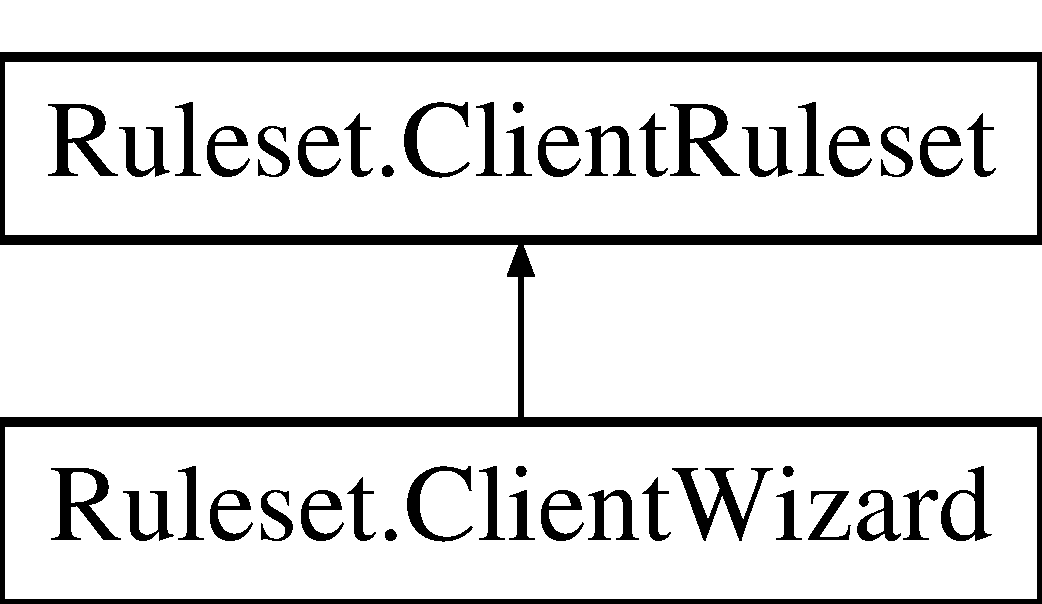
\includegraphics[height=2.000000cm]{a00016}
\end{center}
\end{figure}
\subsubsection*{Öffentliche Methoden}
\begin{DoxyCompactItemize}
\item 
\hyperlink{a00013}{Player\-State} \hyperlink{a00016_a473a55c851bbda707b25948c39334a8a}{get\-Current\-Player} ()
\item 
\hyperlink{a00013}{Player\-State} \hyperlink{a00016_a4a5e3a0fa28ba2bd563224d875f5835c}{get\-Player\-State} (String name)
\item 
void \hyperlink{a00016_afcfbddd7397a6043913b5e742934d2c2}{resolve\-Message} (Msg\-Card msg\-Card, String name)
\item 
void \hyperlink{a00016_ac639a8d99c0e2243f9f3fe565a315c51}{resolve\-Message} (Msg\-Multi\-Cards msg\-Multi\-Card, String name)
\item 
void \hyperlink{a00016_a9f1a95cc9488d8a9519ce69718f91322}{resolve\-Message} (Msg\-Number msg\-Number, String name)
\item 
void \hyperlink{a00016_ada2667ea093481a58f253f43ff6cc49f}{resolve\-Message} (Msg\-Selection msg\-Selection, String name)
\item 
Msg\-Card\-Request \hyperlink{a00016_a03936d0652a15f647fb42651e475b950}{send\-Card\-Request} (String name)
\end{DoxyCompactItemize}


\subsubsection{Ausführliche Beschreibung}
Das \hyperlink{a00016}{Server\-Ruleset} wird im Game\-Server instanziert und verwaltet die Zust�nde des Game\-States im Server. Mit der Methode \hyperlink{a00016_aa49663b89f89b9f7b3685f0b96560f69}{is\-Valid\-Move()} wird eine Eingabe eines Clients auf Regelkonformit�t �berpr�ft und dann im Game\-Server das \hyperlink{a00008}{Game\-State} ver�ndert. �ber \hyperlink{a00016_afcfbddd7397a6043913b5e742934d2c2}{resolve\-Message()} kann eine Game\-Serverinstanz eine Ruleset\-Message vom Player an das Ruleset weiterleiten. 

\subsubsection{Dokumentation der Elementfunktionen}
\hypertarget{a00016_a473a55c851bbda707b25948c39334a8a}{\index{Ruleset\-::\-Server\-Ruleset@{Ruleset\-::\-Server\-Ruleset}!get\-Current\-Player@{get\-Current\-Player}}
\index{get\-Current\-Player@{get\-Current\-Player}!Ruleset::ServerRuleset@{Ruleset\-::\-Server\-Ruleset}}
\paragraph[{get\-Current\-Player}]{\setlength{\rightskip}{0pt plus 5cm}{\bf Player\-State} Ruleset.\-Server\-Ruleset.\-get\-Current\-Player (
\begin{DoxyParamCaption}
{}
\end{DoxyParamCaption}
)}}\label{a00016_a473a55c851bbda707b25948c39334a8a}


Holt den Spieler der gerade am Zug ist. 

\begin{DoxyReturn}{Rückgabe}
current\-Player Der Spielzustand des Spielers der grad am Zug ist 
\end{DoxyReturn}
\hypertarget{a00016_a4a5e3a0fa28ba2bd563224d875f5835c}{\index{Ruleset\-::\-Server\-Ruleset@{Ruleset\-::\-Server\-Ruleset}!get\-Player\-State@{get\-Player\-State}}
\index{get\-Player\-State@{get\-Player\-State}!Ruleset::ServerRuleset@{Ruleset\-::\-Server\-Ruleset}}
\paragraph[{get\-Player\-State}]{\setlength{\rightskip}{0pt plus 5cm}{\bf Player\-State} Ruleset.\-Server\-Ruleset.\-get\-Player\-State (
\begin{DoxyParamCaption}
\item[{String}]{name}
\end{DoxyParamCaption}
)}}\label{a00016_a4a5e3a0fa28ba2bd563224d875f5835c}


Holt den Spielerzustand eines Spielers. 


\begin{DoxyParams}{Parameter}
{\em name} & Der Name des Spielers \\
\hline
\end{DoxyParams}
\begin{DoxyReturn}{Rückgabe}
player\-State Spielzustand eines Spielers 
\end{DoxyReturn}
\hypertarget{a00016_afcfbddd7397a6043913b5e742934d2c2}{\index{Ruleset\-::\-Server\-Ruleset@{Ruleset\-::\-Server\-Ruleset}!resolve\-Message@{resolve\-Message}}
\index{resolve\-Message@{resolve\-Message}!Ruleset::ServerRuleset@{Ruleset\-::\-Server\-Ruleset}}
\paragraph[{resolve\-Message}]{\setlength{\rightskip}{0pt plus 5cm}void Ruleset.\-Server\-Ruleset.\-resolve\-Message (
\begin{DoxyParamCaption}
\item[{Msg\-Card}]{msg\-Card, }
\item[{String}]{name}
\end{DoxyParamCaption}
)}}\label{a00016_afcfbddd7397a6043913b5e742934d2c2}


Verarbeitet die Ruleset\-Message dass eine Karte vom Spieler gespielt. 


\begin{DoxyParams}{Parameter}
{\em msg\-Card} & Die Nachricht vom Client welche Karte gespielt wurde \\
\hline
{\em name} & Der Name des Spielers \\
\hline
\end{DoxyParams}
\hypertarget{a00016_ac639a8d99c0e2243f9f3fe565a315c51}{\index{Ruleset\-::\-Server\-Ruleset@{Ruleset\-::\-Server\-Ruleset}!resolve\-Message@{resolve\-Message}}
\index{resolve\-Message@{resolve\-Message}!Ruleset::ServerRuleset@{Ruleset\-::\-Server\-Ruleset}}
\paragraph[{resolve\-Message}]{\setlength{\rightskip}{0pt plus 5cm}void Ruleset.\-Server\-Ruleset.\-resolve\-Message (
\begin{DoxyParamCaption}
\item[{Msg\-Multi\-Cards}]{msg\-Multi\-Card, }
\item[{String}]{name}
\end{DoxyParamCaption}
)}}\label{a00016_ac639a8d99c0e2243f9f3fe565a315c51}


Verarbeitet die Ruleset\-Message dass mehrere Karten von einem Spieler �bergeben wurden. 


\begin{DoxyParams}{Parameter}
{\em msg\-Multi\-Card} & Die Nachricht vom Client \\
\hline
{\em name} & Der Name des Spielers \\
\hline
\end{DoxyParams}
\hypertarget{a00016_a9f1a95cc9488d8a9519ce69718f91322}{\index{Ruleset\-::\-Server\-Ruleset@{Ruleset\-::\-Server\-Ruleset}!resolve\-Message@{resolve\-Message}}
\index{resolve\-Message@{resolve\-Message}!Ruleset::ServerRuleset@{Ruleset\-::\-Server\-Ruleset}}
\paragraph[{resolve\-Message}]{\setlength{\rightskip}{0pt plus 5cm}void Ruleset.\-Server\-Ruleset.\-resolve\-Message (
\begin{DoxyParamCaption}
\item[{Msg\-Number}]{msg\-Number, }
\item[{String}]{name}
\end{DoxyParamCaption}
)}}\label{a00016_a9f1a95cc9488d8a9519ce69718f91322}


Verarbeitet die Ruleset\-Message dass ein Spieler eine Stichangabe gemacht hat. 


\begin{DoxyParams}{Parameter}
{\em msg\-Number} & Die Nachricht vom Client \\
\hline
{\em name} & Der Name des Spielers \\
\hline
\end{DoxyParams}
\hypertarget{a00016_ada2667ea093481a58f253f43ff6cc49f}{\index{Ruleset\-::\-Server\-Ruleset@{Ruleset\-::\-Server\-Ruleset}!resolve\-Message@{resolve\-Message}}
\index{resolve\-Message@{resolve\-Message}!Ruleset::ServerRuleset@{Ruleset\-::\-Server\-Ruleset}}
\paragraph[{resolve\-Message}]{\setlength{\rightskip}{0pt plus 5cm}void Ruleset.\-Server\-Ruleset.\-resolve\-Message (
\begin{DoxyParamCaption}
\item[{Msg\-Selection}]{msg\-Selection, }
\item[{String}]{name}
\end{DoxyParamCaption}
)}}\label{a00016_ada2667ea093481a58f253f43ff6cc49f}


Verarbeitet die Ruleset\-Message dass ein Spieler eine Farbe ausgew�hlt hat. 


\begin{DoxyParams}{Parameter}
{\em msg\-Selection} & Die Nachricht vom Client \\
\hline
{\em name} & \\
\hline
\end{DoxyParams}
\hypertarget{a00016_a03936d0652a15f647fb42651e475b950}{\index{Ruleset\-::\-Server\-Ruleset@{Ruleset\-::\-Server\-Ruleset}!send\-Card\-Request@{send\-Card\-Request}}
\index{send\-Card\-Request@{send\-Card\-Request}!Ruleset::ServerRuleset@{Ruleset\-::\-Server\-Ruleset}}
\paragraph[{send\-Card\-Request}]{\setlength{\rightskip}{0pt plus 5cm}Msg\-Card\-Request Ruleset.\-Server\-Ruleset.\-send\-Card\-Request (
\begin{DoxyParamCaption}
\item[{String}]{name}
\end{DoxyParamCaption}
)}}\label{a00016_a03936d0652a15f647fb42651e475b950}


Schickt einem Spieler die Aufforderung eine Karte zu spielen. 


\begin{DoxyParams}{Parameter}
{\em name} & Name des Spielers \\
\hline
\end{DoxyParams}
\begin{DoxyReturn}{Rückgabe}
new Msg\-Card\-Request() Eine Nachricht an den Spieler 
\end{DoxyReturn}

\hypertarget{a00017}{\subsection{Ruleset.\-Server\-Wizard Klassenreferenz}
\label{a00017}\index{Ruleset.\-Server\-Wizard@{Ruleset.\-Server\-Wizard}}
}
Klassendiagramm für Ruleset.\-Server\-Wizard\-:\begin{figure}[H]
\begin{center}
\leavevmode
\includegraphics[height=2.000000cm]{a00017}
\end{center}
\end{figure}
\subsubsection*{Öffentliche Methoden}
\begin{DoxyCompactItemize}
\item 
boolean \hyperlink{a00017_af079641e9a83d29de9e1ac868a0af202}{is\-Valid\-Move} (\hyperlink{a00001}{Card} card)
\item 
Msg\-Number\-Request \hyperlink{a00017_af6af06ed2f091d30df603c27549e3f88}{send\-Number\-Request} (String name)
\item 
Msg\-Selection\-Request \hyperlink{a00017_a1b291eecc620aa8dda228e6d7cf6a595}{send\-Selection\-Request} (String name)
\end{DoxyCompactItemize}


\subsubsection{Ausführliche Beschreibung}
Sie enth�lt zudem weitere Methoden, welche f�r das Spiel Wizard spezifisch ben�tigt werden, wie das Bestimmen einer Trumpffarbe und die Bestimmung der Rundenanzahl. 

\subsubsection{Dokumentation der Elementfunktionen}
\hypertarget{a00017_af079641e9a83d29de9e1ac868a0af202}{\index{Ruleset\-::\-Server\-Wizard@{Ruleset\-::\-Server\-Wizard}!is\-Valid\-Move@{is\-Valid\-Move}}
\index{is\-Valid\-Move@{is\-Valid\-Move}!Ruleset::ServerWizard@{Ruleset\-::\-Server\-Wizard}}
\paragraph[{is\-Valid\-Move}]{\setlength{\rightskip}{0pt plus 5cm}boolean Ruleset.\-Server\-Wizard.\-is\-Valid\-Move (
\begin{DoxyParamCaption}
\item[{{\bf Card}}]{card}
\end{DoxyParamCaption}
)\hspace{0.3cm}{\ttfamily [virtual]}}}\label{a00017_af079641e9a83d29de9e1ac868a0af202}


Pr�ft ob ein gemachter Zug in einem Wizard Spiel g�ltig ist. 

\begin{DoxyReturn}{Rückgabe}
is\-Valid true falls Zug g�ltig, false wenn nicht 
\end{DoxyReturn}


Implementiert \hyperlink{a00016_aa49663b89f89b9f7b3685f0b96560f69}{Ruleset.\-Server\-Ruleset}.

\hypertarget{a00017_af6af06ed2f091d30df603c27549e3f88}{\index{Ruleset\-::\-Server\-Wizard@{Ruleset\-::\-Server\-Wizard}!send\-Number\-Request@{send\-Number\-Request}}
\index{send\-Number\-Request@{send\-Number\-Request}!Ruleset::ServerWizard@{Ruleset\-::\-Server\-Wizard}}
\paragraph[{send\-Number\-Request}]{\setlength{\rightskip}{0pt plus 5cm}Msg\-Number\-Request Ruleset.\-Server\-Wizard.\-send\-Number\-Request (
\begin{DoxyParamCaption}
\item[{String}]{name}
\end{DoxyParamCaption}
)}}\label{a00017_af6af06ed2f091d30df603c27549e3f88}


Schickt einem Spieler die Aufforderung eine Stichanzahl anzugeben. 


\begin{DoxyParams}{Parameter}
{\em name} & Name des Spielers \\
\hline
\end{DoxyParams}
\begin{DoxyReturn}{Rückgabe}
new Msg\-Number\-Request() Eine Nachricht an den Spieler 
\end{DoxyReturn}
\hypertarget{a00017_a1b291eecc620aa8dda228e6d7cf6a595}{\index{Ruleset\-::\-Server\-Wizard@{Ruleset\-::\-Server\-Wizard}!send\-Selection\-Request@{send\-Selection\-Request}}
\index{send\-Selection\-Request@{send\-Selection\-Request}!Ruleset::ServerWizard@{Ruleset\-::\-Server\-Wizard}}
\paragraph[{send\-Selection\-Request}]{\setlength{\rightskip}{0pt plus 5cm}Msg\-Selection\-Request Ruleset.\-Server\-Wizard.\-send\-Selection\-Request (
\begin{DoxyParamCaption}
\item[{String}]{name}
\end{DoxyParamCaption}
)}}\label{a00017_a1b291eecc620aa8dda228e6d7cf6a595}


Schickt einem Spieler die Aufforderung eine Farbe zu w�hlen. 


\begin{DoxyParams}{Parameter}
{\em name} & Name des Spielers \\
\hline
\end{DoxyParams}
\begin{DoxyReturn}{Rückgabe}
new Msg\-Selection\-Request() Eine Nachricht an den Spieler 
\end{DoxyReturn}

\hypertarget{a00018}{\subsection{Com\-Objects.\-Com\-Been\-Kicked Klassenreferenz}
\label{a00018}\index{Com\-Objects.\-Com\-Been\-Kicked@{Com\-Objects.\-Com\-Been\-Kicked}}
}
\subsubsection*{Öffentliche Methoden}
\begin{DoxyCompactItemize}
\item 
\hyperlink{a00018_a6cfa1081f4ec243a339ec8d52a770d17}{Com\-Been\-Kicked} (String message)
\item 
String \hyperlink{a00018_ab71e06326d507463a4e6c1f08b50c089}{get\-Message} ()
\end{DoxyCompactItemize}


\subsubsection{Ausführliche Beschreibung}
Die Nachricht wird an einen Spieler gesendet, wenn er aus einem Spiel erntfernt wurde. Dies geschieht, wenn ein Spieler ein Spiel verlässt oder wenn der Spielleiter das Wartefenster verlässt. 

\subsubsection{Beschreibung der Konstruktoren und Destruktoren}
\hypertarget{a00018_a6cfa1081f4ec243a339ec8d52a770d17}{\index{Com\-Objects\-::\-Com\-Been\-Kicked@{Com\-Objects\-::\-Com\-Been\-Kicked}!Com\-Been\-Kicked@{Com\-Been\-Kicked}}
\index{Com\-Been\-Kicked@{Com\-Been\-Kicked}!ComObjects::ComBeenKicked@{Com\-Objects\-::\-Com\-Been\-Kicked}}
\paragraph[{Com\-Been\-Kicked}]{\setlength{\rightskip}{0pt plus 5cm}Com\-Objects.\-Com\-Been\-Kicked.\-Com\-Been\-Kicked (
\begin{DoxyParamCaption}
\item[{String}]{message}
\end{DoxyParamCaption}
)}}\label{a00018_a6cfa1081f4ec243a339ec8d52a770d17}


Dies ist der Kontruktor für eine neue Com\-Been\-Kicked-\/\-Nachricht. 


\begin{DoxyParams}{Parameter}
{\em message} & ist die Nachricht. \\
\hline
\end{DoxyParams}


\subsubsection{Dokumentation der Elementfunktionen}
\hypertarget{a00018_ab71e06326d507463a4e6c1f08b50c089}{\index{Com\-Objects\-::\-Com\-Been\-Kicked@{Com\-Objects\-::\-Com\-Been\-Kicked}!get\-Message@{get\-Message}}
\index{get\-Message@{get\-Message}!ComObjects::ComBeenKicked@{Com\-Objects\-::\-Com\-Been\-Kicked}}
\paragraph[{get\-Message}]{\setlength{\rightskip}{0pt plus 5cm}String Com\-Objects.\-Com\-Been\-Kicked.\-get\-Message (
\begin{DoxyParamCaption}
{}
\end{DoxyParamCaption}
)}}\label{a00018_ab71e06326d507463a4e6c1f08b50c089}


Diese Methode liefert die Nachricht, die an den Spieler gesendet wird, wenn er entfernt wird. 

\begin{DoxyReturn}{Rückgabe}
die Nachricht. 
\end{DoxyReturn}

\hypertarget{a00019}{\subsection{Com\-Objects.\-Com\-Chat\-Message Klassenreferenz}
\label{a00019}\index{Com\-Objects.\-Com\-Chat\-Message@{Com\-Objects.\-Com\-Chat\-Message}}
}
Klassendiagramm für Com\-Objects.\-Com\-Chat\-Message\-:\begin{figure}[H]
\begin{center}
\leavevmode
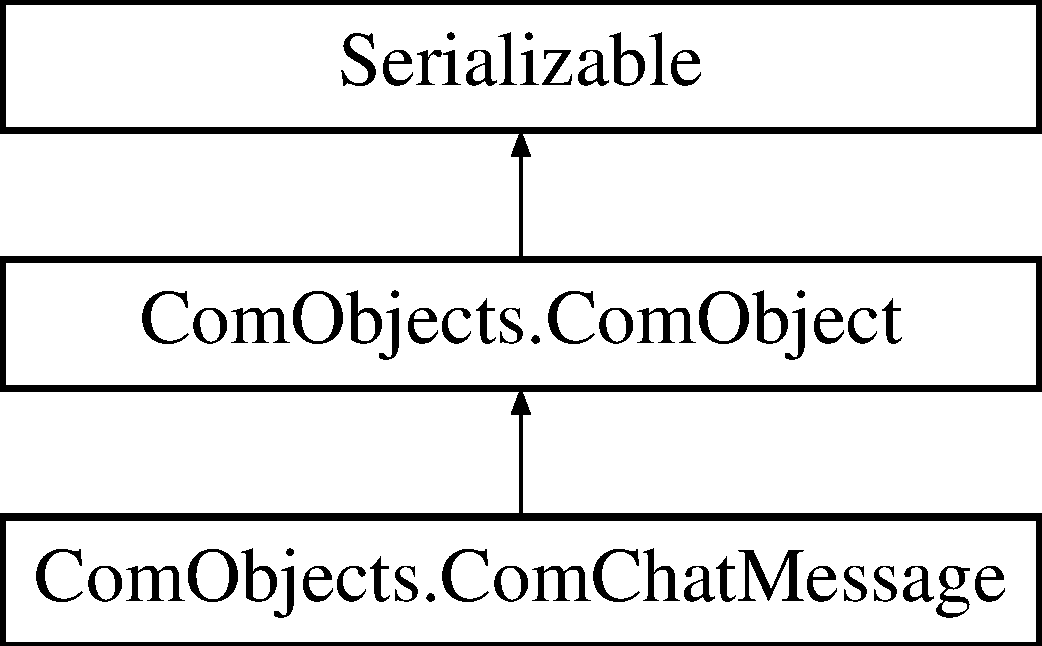
\includegraphics[height=3.000000cm]{a00019}
\end{center}
\end{figure}
\subsubsection*{Öffentliche Methoden}
\begin{DoxyCompactItemize}
\item 
\hyperlink{a00019_a63e61e963a46a919644731bcc41a3c6a}{Com\-Chat\-Message} (String message)
\item 
String \hyperlink{a00019_ac8574b456968ef6c4e5d56a1f453d823}{get\-Chat\-Message} ()
\end{DoxyCompactItemize}


\subsubsection{Ausführliche Beschreibung}
Sie enthält eine Chatnachricht in Form eines Strings. 

\subsubsection{Beschreibung der Konstruktoren und Destruktoren}
\hypertarget{a00019_a63e61e963a46a919644731bcc41a3c6a}{\index{Com\-Objects\-::\-Com\-Chat\-Message@{Com\-Objects\-::\-Com\-Chat\-Message}!Com\-Chat\-Message@{Com\-Chat\-Message}}
\index{Com\-Chat\-Message@{Com\-Chat\-Message}!ComObjects::ComChatMessage@{Com\-Objects\-::\-Com\-Chat\-Message}}
\paragraph[{Com\-Chat\-Message}]{\setlength{\rightskip}{0pt plus 5cm}Com\-Objects.\-Com\-Chat\-Message.\-Com\-Chat\-Message (
\begin{DoxyParamCaption}
\item[{String}]{message}
\end{DoxyParamCaption}
)}}\label{a00019_a63e61e963a46a919644731bcc41a3c6a}


Dies ist der Kontruktor für eine neue Com\-Chat\-Message-\/\-Nachricht. 


\begin{DoxyParams}{Parameter}
{\em message} & ist die Chatnachricht, die versendet wird. \\
\hline
\end{DoxyParams}


\subsubsection{Dokumentation der Elementfunktionen}
\hypertarget{a00019_ac8574b456968ef6c4e5d56a1f453d823}{\index{Com\-Objects\-::\-Com\-Chat\-Message@{Com\-Objects\-::\-Com\-Chat\-Message}!get\-Chat\-Message@{get\-Chat\-Message}}
\index{get\-Chat\-Message@{get\-Chat\-Message}!ComObjects::ComChatMessage@{Com\-Objects\-::\-Com\-Chat\-Message}}
\paragraph[{get\-Chat\-Message}]{\setlength{\rightskip}{0pt plus 5cm}String Com\-Objects.\-Com\-Chat\-Message.\-get\-Chat\-Message (
\begin{DoxyParamCaption}
{}
\end{DoxyParamCaption}
)}}\label{a00019_ac8574b456968ef6c4e5d56a1f453d823}


Hier kann die versendete Nachricht von anderen Klassen ausgelesen werden. 

\begin{DoxyReturn}{Rückgabe}
die Chatnachricht, die versendet wurde. 
\end{DoxyReturn}

\hypertarget{a00020}{\subsection{Ruleset.\-Wiz\-I\-D Enum-\/\-Referenz}
\label{a00020}\index{Ruleset.\-Wiz\-I\-D@{Ruleset.\-Wiz\-I\-D}}
}

\hypertarget{a00021}{\subsection{Com\-Objects.\-Com\-Client\-Quit Klassenreferenz}
\label{a00021}\index{Com\-Objects.\-Com\-Client\-Quit@{Com\-Objects.\-Com\-Client\-Quit}}
}
Klassendiagramm für Com\-Objects.\-Com\-Client\-Quit\-:\begin{figure}[H]
\begin{center}
\leavevmode
\includegraphics[height=3.000000cm]{a00021}
\end{center}
\end{figure}


\subsubsection{Ausführliche Beschreibung}
Die Nachricht wird verschickt, wenn der Spieler ein Fenster schließt. 
\hypertarget{a00022}{\subsection{Com\-Objects.\-Com\-Create\-Game\-Request Klassenreferenz}
\label{a00022}\index{Com\-Objects.\-Com\-Create\-Game\-Request@{Com\-Objects.\-Com\-Create\-Game\-Request}}
}
Klassendiagramm für Com\-Objects.\-Com\-Create\-Game\-Request\-:\begin{figure}[H]
\begin{center}
\leavevmode
\includegraphics[height=3.000000cm]{a00022}
\end{center}
\end{figure}
\subsubsection*{Öffentliche Methoden}
\begin{DoxyCompactItemize}
\item 
\hyperlink{a00022_aaf1ae68768968cb49221f0c29837dffa}{Com\-Create\-Game\-Request} (String name, Enum ruleset, boolean has\-Password, String password)
\item 
String \hyperlink{a00022_a06976fffc41a66420d249b068106640e}{get\-Game\-Name} ()
\item 
Enum \hyperlink{a00022_a122cf6895c8ea900d838ce798350730c}{get\-Ruleset} ()
\item 
boolean \hyperlink{a00022_afbbb12d942d480dfd1e4f63da4806db5}{has\-Password} ()
\item 
String \hyperlink{a00022_a77cbcd29cffda3d6a312de7a760f7e0e}{get\-Password} ()
\end{DoxyCompactItemize}


\subsubsection{Ausführliche Beschreibung}
Diese Nachricht wird versendet, wenn ein neues Spiel erstellt werden soll. 

\subsubsection{Beschreibung der Konstruktoren und Destruktoren}
\hypertarget{a00022_aaf1ae68768968cb49221f0c29837dffa}{\index{Com\-Objects\-::\-Com\-Create\-Game\-Request@{Com\-Objects\-::\-Com\-Create\-Game\-Request}!Com\-Create\-Game\-Request@{Com\-Create\-Game\-Request}}
\index{Com\-Create\-Game\-Request@{Com\-Create\-Game\-Request}!ComObjects::ComCreateGameRequest@{Com\-Objects\-::\-Com\-Create\-Game\-Request}}
\paragraph[{Com\-Create\-Game\-Request}]{\setlength{\rightskip}{0pt plus 5cm}Com\-Objects.\-Com\-Create\-Game\-Request.\-Com\-Create\-Game\-Request (
\begin{DoxyParamCaption}
\item[{String}]{name, }
\item[{Enum}]{ruleset, }
\item[{boolean}]{has\-Password, }
\item[{String}]{password}
\end{DoxyParamCaption}
)}}\label{a00022_aaf1ae68768968cb49221f0c29837dffa}


Dies ist der Kontruktor für eine neue Com\-Create\-Game\-Request-\/\-Nachricht. 


\begin{DoxyParams}{Parameter}
{\em name} & ist der Name des Spiels. \\
\hline
{\em ruleset} & ist die der Spieltyp, der erstellt werden soll. \\
\hline
{\em has\-Password} & sagt, ob ein Passwort gesetzt wurde. \\
\hline
{\em password} & ist das Passwort, das gesetzt wurde. \\
\hline
\end{DoxyParams}


Benutzt Com\-Objects.\-Com\-Create\-Game\-Request.\-has\-Password().



\subsubsection{Dokumentation der Elementfunktionen}
\hypertarget{a00022_a06976fffc41a66420d249b068106640e}{\index{Com\-Objects\-::\-Com\-Create\-Game\-Request@{Com\-Objects\-::\-Com\-Create\-Game\-Request}!get\-Game\-Name@{get\-Game\-Name}}
\index{get\-Game\-Name@{get\-Game\-Name}!ComObjects::ComCreateGameRequest@{Com\-Objects\-::\-Com\-Create\-Game\-Request}}
\paragraph[{get\-Game\-Name}]{\setlength{\rightskip}{0pt plus 5cm}String Com\-Objects.\-Com\-Create\-Game\-Request.\-get\-Game\-Name (
\begin{DoxyParamCaption}
{}
\end{DoxyParamCaption}
)}}\label{a00022_a06976fffc41a66420d249b068106640e}


Diese Methode gibt den Namen des Spiels zurück. 

\begin{DoxyReturn}{Rückgabe}
den Spielnamen. 
\end{DoxyReturn}
\hypertarget{a00022_a77cbcd29cffda3d6a312de7a760f7e0e}{\index{Com\-Objects\-::\-Com\-Create\-Game\-Request@{Com\-Objects\-::\-Com\-Create\-Game\-Request}!get\-Password@{get\-Password}}
\index{get\-Password@{get\-Password}!ComObjects::ComCreateGameRequest@{Com\-Objects\-::\-Com\-Create\-Game\-Request}}
\paragraph[{get\-Password}]{\setlength{\rightskip}{0pt plus 5cm}String Com\-Objects.\-Com\-Create\-Game\-Request.\-get\-Password (
\begin{DoxyParamCaption}
{}
\end{DoxyParamCaption}
)}}\label{a00022_a77cbcd29cffda3d6a312de7a760f7e0e}


Gibt das Passwort zurück. 

Sollte keines gesetzt sein, wird null zurück gegeben. \begin{DoxyReturn}{Rückgabe}
das Passwort. 
\end{DoxyReturn}
\hypertarget{a00022_a122cf6895c8ea900d838ce798350730c}{\index{Com\-Objects\-::\-Com\-Create\-Game\-Request@{Com\-Objects\-::\-Com\-Create\-Game\-Request}!get\-Ruleset@{get\-Ruleset}}
\index{get\-Ruleset@{get\-Ruleset}!ComObjects::ComCreateGameRequest@{Com\-Objects\-::\-Com\-Create\-Game\-Request}}
\paragraph[{get\-Ruleset}]{\setlength{\rightskip}{0pt plus 5cm}Enum Com\-Objects.\-Com\-Create\-Game\-Request.\-get\-Ruleset (
\begin{DoxyParamCaption}
{}
\end{DoxyParamCaption}
)}}\label{a00022_a122cf6895c8ea900d838ce798350730c}


Diese Methode gibt das Regelwerk zurück, das benutzt werden soll. 

\begin{DoxyReturn}{Rückgabe}
das Regelwerk, welches benutzt wird. 
\end{DoxyReturn}
\hypertarget{a00022_afbbb12d942d480dfd1e4f63da4806db5}{\index{Com\-Objects\-::\-Com\-Create\-Game\-Request@{Com\-Objects\-::\-Com\-Create\-Game\-Request}!has\-Password@{has\-Password}}
\index{has\-Password@{has\-Password}!ComObjects::ComCreateGameRequest@{Com\-Objects\-::\-Com\-Create\-Game\-Request}}
\paragraph[{has\-Password}]{\setlength{\rightskip}{0pt plus 5cm}boolean Com\-Objects.\-Com\-Create\-Game\-Request.\-has\-Password (
\begin{DoxyParamCaption}
{}
\end{DoxyParamCaption}
)}}\label{a00022_afbbb12d942d480dfd1e4f63da4806db5}


Diese Methode gibt an, ob eine Passwort für ein Spiel gesetzt wurde. 

\begin{DoxyReturn}{Rückgabe}
ob es ein Passwort gibt. 
\end{DoxyReturn}


Wird benutzt von Com\-Objects.\-Com\-Create\-Game\-Request.\-Com\-Create\-Game\-Request().


\hypertarget{a00023}{\subsection{Com\-Objects.\-Com\-Init\-Game\-Lobby Klassenreferenz}
\label{a00023}\index{Com\-Objects.\-Com\-Init\-Game\-Lobby@{Com\-Objects.\-Com\-Init\-Game\-Lobby}}
}
Klassendiagramm für Com\-Objects.\-Com\-Init\-Game\-Lobby\-:\begin{figure}[H]
\begin{center}
\leavevmode
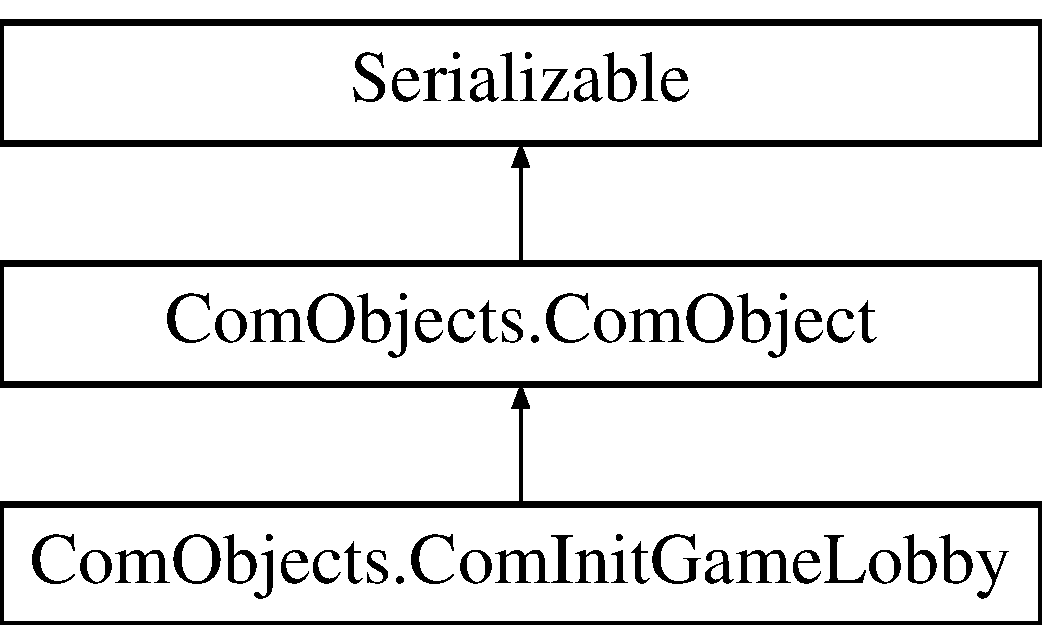
\includegraphics[height=3.000000cm]{a00023}
\end{center}
\end{figure}
\subsubsection*{Öffentliche Methoden}
\begin{DoxyCompactItemize}
\item 
\hyperlink{a00023_ab00f0be4143765950c60ff13a3a0216a}{Com\-Init\-Game\-Lobby} (List player\-List)
\item 
Object \hyperlink{a00023_a9922020c95b5b0173fe00c7f2862ae0c}{get\-Player\-List} ()
\end{DoxyCompactItemize}


\subsubsection{Ausführliche Beschreibung}
Sie liefert die Liste der Spieler, die sich bereits beim Betreten des Wartefensters darin befinden. 

\subsubsection{Beschreibung der Konstruktoren und Destruktoren}
\hypertarget{a00023_ab00f0be4143765950c60ff13a3a0216a}{\index{Com\-Objects\-::\-Com\-Init\-Game\-Lobby@{Com\-Objects\-::\-Com\-Init\-Game\-Lobby}!Com\-Init\-Game\-Lobby@{Com\-Init\-Game\-Lobby}}
\index{Com\-Init\-Game\-Lobby@{Com\-Init\-Game\-Lobby}!ComObjects::ComInitGameLobby@{Com\-Objects\-::\-Com\-Init\-Game\-Lobby}}
\paragraph[{Com\-Init\-Game\-Lobby}]{\setlength{\rightskip}{0pt plus 5cm}Com\-Objects.\-Com\-Init\-Game\-Lobby.\-Com\-Init\-Game\-Lobby (
\begin{DoxyParamCaption}
\item[{List}]{player\-List}
\end{DoxyParamCaption}
)}}\label{a00023_ab00f0be4143765950c60ff13a3a0216a}


Dies ist der Kontruktor für eine neue Com\-Init\-Game\-Lobby-\/\-Nachricht. 


\begin{DoxyParams}{Parameter}
{\em player\-List} & ist die Liste aller Player, die sich im Wartefenster befinden. \\
\hline
\end{DoxyParams}


\subsubsection{Dokumentation der Elementfunktionen}
\hypertarget{a00023_a9922020c95b5b0173fe00c7f2862ae0c}{\index{Com\-Objects\-::\-Com\-Init\-Game\-Lobby@{Com\-Objects\-::\-Com\-Init\-Game\-Lobby}!get\-Player\-List@{get\-Player\-List}}
\index{get\-Player\-List@{get\-Player\-List}!ComObjects::ComInitGameLobby@{Com\-Objects\-::\-Com\-Init\-Game\-Lobby}}
\paragraph[{get\-Player\-List}]{\setlength{\rightskip}{0pt plus 5cm}Object Com\-Objects.\-Com\-Init\-Game\-Lobby.\-get\-Player\-List (
\begin{DoxyParamCaption}
{}
\end{DoxyParamCaption}
)}}\label{a00023_a9922020c95b5b0173fe00c7f2862ae0c}


Diese Methode gibt die Liste der Player zurück, die sich momentan inm Wartefenster befinden. 

\begin{DoxyReturn}{Rückgabe}
die Liste der Spieler. 
\end{DoxyReturn}

\hypertarget{a00024}{\subsection{View\-Notification Enum-\/\-Referenz}
\label{a00024}\index{View\-Notification@{View\-Notification}}
}
\subsubsection*{Öffentliche Attribute}
\begin{DoxyCompactItemize}
\item 
\hypertarget{a00024_a71398de7d7d0c05607093b90c17413bd}{{\bfseries move\-Acknowledged}}\label{a00024_a71398de7d7d0c05607093b90c17413bd}

\item 
\hypertarget{a00024_a0cee4c2ca533a7a49e94671b62b3ea9c}{{\bfseries choose\-Cards\-Successful}}\label{a00024_a0cee4c2ca533a7a49e94671b62b3ea9c}

\item 
\hypertarget{a00024_af9973716fdc25af45be6ce4725f3242d}{{\bfseries Input\-Number\-Successful}}\label{a00024_af9973716fdc25af45be6ce4725f3242d}

\item 
\hypertarget{a00024_a0ac1481b30289078afff8df2d8509e55}{{\bfseries choose\-Item\-Successful}}\label{a00024_a0ac1481b30289078afff8df2d8509e55}

\item 
\hypertarget{a00024_ab94d68b95b582b7cfb4b06c0601a8617}{{\bfseries player\-List\-Update}}\label{a00024_ab94d68b95b582b7cfb4b06c0601a8617}

\item 
\hypertarget{a00024_a52a96b472bb537904d3bad951bb106f5}{{\bfseries game\-List\-Update}}\label{a00024_a52a96b472bb537904d3bad951bb106f5}

\item 
\hypertarget{a00024_ab8055439fa39ac19535cc7eb48f3b528}{{\bfseries chat\-Message}}\label{a00024_ab8055439fa39ac19535cc7eb48f3b528}

\item 
\hypertarget{a00024_aa7d623b699d34c703cdb5a3bf507acc8}{{\bfseries login\-Succesful}}\label{a00024_aa7d623b699d34c703cdb5a3bf507acc8}

\item 
\hypertarget{a00024_a24ee2db83d9ed6d40f839bc235ae860f}{{\bfseries join\-Game\-Succesful}}\label{a00024_a24ee2db83d9ed6d40f839bc235ae860f}

\item 
\hypertarget{a00024_a900922a7746bade569a472e311a27cb7}{{\bfseries game\-Started}}\label{a00024_a900922a7746bade569a472e311a27cb7}

\item 
\hypertarget{a00024_a10126f0d7ab34818a6fcac72e0834f54}{{\bfseries password\-Accepted}}\label{a00024_a10126f0d7ab34818a6fcac72e0834f54}

\item 
\hypertarget{a00024_aaf6d6355be04b40a09ef226c86bf8659}{{\bfseries played\-Cards\-Update}}\label{a00024_aaf6d6355be04b40a09ef226c86bf8659}

\item 
\hypertarget{a00024_a8ae442eff1cd0550d1d97f86d71fd02e}{{\bfseries other\-Data\-Update}}\label{a00024_a8ae442eff1cd0550d1d97f86d71fd02e}

\item 
\hypertarget{a00024_aa10538b6b27362eecff8ef433b1d14c6}{{\bfseries window\-Change\-Forced}}\label{a00024_aa10538b6b27362eecff8ef433b1d14c6}

\item 
\hypertarget{a00024_a874f70629715c6d24776db50c34547e9}{{\bfseries open\-Choose\-Cards}}\label{a00024_a874f70629715c6d24776db50c34547e9}

\item 
\hypertarget{a00024_a70960eb2d8a55fd73166c3d7975fbb70}{{\bfseries open\-Choose\-Item}}\label{a00024_a70960eb2d8a55fd73166c3d7975fbb70}

\item 
\hypertarget{a00024_a8aa5232ad1888872984b3608cfb74705}{{\bfseries open\-Input\-Number}}\label{a00024_a8aa5232ad1888872984b3608cfb74705}

\item 
\hypertarget{a00024_a2fba94db10d6b57caf70c532f16d118f}{{\bfseries open\-Warning}}\label{a00024_a2fba94db10d6b57caf70c532f16d118f}

\item 
\hypertarget{a00024_ac2a087bbbdc94e296fc84945a704898e}{{\bfseries show\-Score}}\label{a00024_ac2a087bbbdc94e296fc84945a704898e}

\end{DoxyCompactItemize}


\subsubsection{Ausführliche Beschreibung}
Enum, das vom \hyperlink{a00003}{Client\-Model} ueber notify an seine Observer geschickt wird, um mitzuteilen, welche Veraenderung stattgefunden hat. 
\hypertarget{a00025}{\subsection{Com\-Been\-Kicked Klassenreferenz}
\label{a00025}\index{Com\-Been\-Kicked@{Com\-Been\-Kicked}}
}


Abgeleitet von \hyperlink{a00037}{Com\-Object} und Serializable.

\subsubsection*{Öffentliche Methoden}
\begin{DoxyCompactItemize}
\item 
\hyperlink{a00025_a62d740de69f8a07fdcd3817754fc616e}{Com\-Been\-Kicked} (String message)
\item 
String \hyperlink{a00025_afafd068b736520af1e24269a284980a9}{get\-Message} ()
\item 
void \hyperlink{a00025_a758d7005755a181717f238f714d87dd2}{process} (\hyperlink{a00003}{Client\-Model} model)
\item 
void \hyperlink{a00025_ac67b5ce3ec03d48ef1e6caad6e49c902}{process} (\hyperlink{a00076}{Player} player, \hyperlink{a00077}{Server} server)
\end{DoxyCompactItemize}
\subsubsection*{Private Attribute}
\begin{DoxyCompactItemize}
\item 
\hypertarget{a00025_a2836db0f8ae4563c70935b5e514bdc21}{String {\bfseries message}}\label{a00025_a2836db0f8ae4563c70935b5e514bdc21}

\end{DoxyCompactItemize}


\subsubsection{Ausführliche Beschreibung}
Diese Klasse ist ein spezielles Kommunikations-\/\-Objekt. Die Nachricht wird an einen Spieler gesendet, wenn er aus einem Spiel erntfernt wurde. Dies geschieht, wenn ein Spieler ein Spiel verlaesst oder wenn der Spielleiter das Wartefenster verlaesst. 

\subsubsection{Beschreibung der Konstruktoren und Destruktoren}
\hypertarget{a00025_a62d740de69f8a07fdcd3817754fc616e}{\index{Com\-Objects\-::\-Com\-Been\-Kicked@{Com\-Objects\-::\-Com\-Been\-Kicked}!Com\-Been\-Kicked@{Com\-Been\-Kicked}}
\index{Com\-Been\-Kicked@{Com\-Been\-Kicked}!ComObjects::ComBeenKicked@{Com\-Objects\-::\-Com\-Been\-Kicked}}
\paragraph[{Com\-Been\-Kicked}]{\setlength{\rightskip}{0pt plus 5cm}{\bf Com\-Been\-Kicked} (
\begin{DoxyParamCaption}
\item[{String}]{message}
\end{DoxyParamCaption}
)}}\label{a00025_a62d740de69f8a07fdcd3817754fc616e}


Dies ist der Kontruktor fuer eine neue Com\-Been\-Kicked-\/\-Nachricht. 


\begin{DoxyParams}{Parameter}
{\em message} & ist die Nachricht. \\
\hline
\end{DoxyParams}


\subsubsection{Dokumentation der Elementfunktionen}
\hypertarget{a00025_afafd068b736520af1e24269a284980a9}{\index{Com\-Objects\-::\-Com\-Been\-Kicked@{Com\-Objects\-::\-Com\-Been\-Kicked}!get\-Message@{get\-Message}}
\index{get\-Message@{get\-Message}!ComObjects::ComBeenKicked@{Com\-Objects\-::\-Com\-Been\-Kicked}}
\paragraph[{get\-Message}]{\setlength{\rightskip}{0pt plus 5cm}String get\-Message (
\begin{DoxyParamCaption}
{}
\end{DoxyParamCaption}
)}}\label{a00025_afafd068b736520af1e24269a284980a9}


Diese Methode liefert die Nachricht, die an den Spieler gesendet wird, wenn er entfernt wird. 

\begin{DoxyReturn}{Rückgabe}
die Nachricht. 
\end{DoxyReturn}
\hypertarget{a00025_a758d7005755a181717f238f714d87dd2}{\index{Com\-Objects\-::\-Com\-Been\-Kicked@{Com\-Objects\-::\-Com\-Been\-Kicked}!process@{process}}
\index{process@{process}!ComObjects::ComBeenKicked@{Com\-Objects\-::\-Com\-Been\-Kicked}}
\paragraph[{process}]{\setlength{\rightskip}{0pt plus 5cm}void process (
\begin{DoxyParamCaption}
\item[{{\bf Client\-Model}}]{model}
\end{DoxyParamCaption}
)}}\label{a00025_a758d7005755a181717f238f714d87dd2}


Diese Methode ist noetig, damit der Client\-Listener\-Thread entscheiden kann welche Message das Object enthaelt und wie diese verarbeitet werden soll. 


\begin{DoxyParams}{Parameter}
{\em model} & ist das Client\-Model, welches übergeben wird, damit die ueberladene Methode richtig gewaehlt wird. \\
\hline
\end{DoxyParams}


Implementiert \hyperlink{a00037_a758d7005755a181717f238f714d87dd2}{Com\-Object}.

\hypertarget{a00025_ac67b5ce3ec03d48ef1e6caad6e49c902}{\index{Com\-Objects\-::\-Com\-Been\-Kicked@{Com\-Objects\-::\-Com\-Been\-Kicked}!process@{process}}
\index{process@{process}!ComObjects::ComBeenKicked@{Com\-Objects\-::\-Com\-Been\-Kicked}}
\paragraph[{process}]{\setlength{\rightskip}{0pt plus 5cm}void process (
\begin{DoxyParamCaption}
\item[{{\bf Player}}]{player, }
\item[{{\bf Server}}]{server}
\end{DoxyParamCaption}
)}}\label{a00025_ac67b5ce3ec03d48ef1e6caad6e49c902}


Diese Methode ist noetig, damit der Thread Player entscheiden kann welche Message das Object enthaelt und wie diese verarbeitet werden soll. 


\begin{DoxyParams}{Parameter}
{\em player} & Der Client welcher den Aufruf startet. \\
\hline
{\em server} & Der Server an den sich das Com\-Objekt weitergibt. \\
\hline
\end{DoxyParams}


Implementiert \hyperlink{a00037_ac67b5ce3ec03d48ef1e6caad6e49c902}{Com\-Object}.


\hypertarget{a00026}{\subsection{Com\-Chat\-Message Klassenreferenz}
\label{a00026}\index{Com\-Chat\-Message@{Com\-Chat\-Message}}
}


Abgeleitet von \hyperlink{a00037}{Com\-Object} und Serializable.

\subsubsection*{Öffentliche Methoden}
\begin{DoxyCompactItemize}
\item 
\hyperlink{a00026_a21a60af1a95931484e5802bb904ef5d5}{Com\-Chat\-Message} (String message)
\item 
String \hyperlink{a00026_a5c7e83aab44b6a6fe19f02ea831f134d}{get\-Chat\-Message} ()
\item 
void \hyperlink{a00026_a758d7005755a181717f238f714d87dd2}{process} (\hyperlink{a00003}{Client\-Model} model)
\item 
void \hyperlink{a00026_ac67b5ce3ec03d48ef1e6caad6e49c902}{process} (\hyperlink{a00076}{Player} player, \hyperlink{a00077}{Server} server)
\end{DoxyCompactItemize}
\subsubsection*{Private Attribute}
\begin{DoxyCompactItemize}
\item 
\hypertarget{a00026_a36925554bcf553be7b9b408466fe794c}{String {\bfseries chat\-Message}}\label{a00026_a36925554bcf553be7b9b408466fe794c}

\end{DoxyCompactItemize}


\subsubsection{Ausführliche Beschreibung}
Diese Klasse ist ein spezielles Kommunikations-\/\-Objekt. Sie enthaelt eine Chatnachricht in Form eines Strings. 

\subsubsection{Beschreibung der Konstruktoren und Destruktoren}
\hypertarget{a00026_a21a60af1a95931484e5802bb904ef5d5}{\index{Com\-Objects\-::\-Com\-Chat\-Message@{Com\-Objects\-::\-Com\-Chat\-Message}!Com\-Chat\-Message@{Com\-Chat\-Message}}
\index{Com\-Chat\-Message@{Com\-Chat\-Message}!ComObjects::ComChatMessage@{Com\-Objects\-::\-Com\-Chat\-Message}}
\paragraph[{Com\-Chat\-Message}]{\setlength{\rightskip}{0pt plus 5cm}{\bf Com\-Chat\-Message} (
\begin{DoxyParamCaption}
\item[{String}]{message}
\end{DoxyParamCaption}
)}}\label{a00026_a21a60af1a95931484e5802bb904ef5d5}


Dies ist der Kontruktor fuer eine neue Com\-Chat\-Message-\/\-Nachricht. 


\begin{DoxyParams}{Parameter}
{\em message} & ist die Chatnachricht, die versendet wird. \\
\hline
\end{DoxyParams}


\subsubsection{Dokumentation der Elementfunktionen}
\hypertarget{a00026_a5c7e83aab44b6a6fe19f02ea831f134d}{\index{Com\-Objects\-::\-Com\-Chat\-Message@{Com\-Objects\-::\-Com\-Chat\-Message}!get\-Chat\-Message@{get\-Chat\-Message}}
\index{get\-Chat\-Message@{get\-Chat\-Message}!ComObjects::ComChatMessage@{Com\-Objects\-::\-Com\-Chat\-Message}}
\paragraph[{get\-Chat\-Message}]{\setlength{\rightskip}{0pt plus 5cm}String get\-Chat\-Message (
\begin{DoxyParamCaption}
{}
\end{DoxyParamCaption}
)}}\label{a00026_a5c7e83aab44b6a6fe19f02ea831f134d}


Hier kann die versendete Nachricht von anderen Klassen ausgelesen werden. 

\begin{DoxyReturn}{Rückgabe}
die Chatnachricht, die versendet wurde. 
\end{DoxyReturn}
\hypertarget{a00026_a758d7005755a181717f238f714d87dd2}{\index{Com\-Objects\-::\-Com\-Chat\-Message@{Com\-Objects\-::\-Com\-Chat\-Message}!process@{process}}
\index{process@{process}!ComObjects::ComChatMessage@{Com\-Objects\-::\-Com\-Chat\-Message}}
\paragraph[{process}]{\setlength{\rightskip}{0pt plus 5cm}void process (
\begin{DoxyParamCaption}
\item[{{\bf Client\-Model}}]{model}
\end{DoxyParamCaption}
)}}\label{a00026_a758d7005755a181717f238f714d87dd2}


Diese Methode ist noetig, damit der Client\-Listener\-Thread entscheiden kann welche Message das Object enthaelt und wie diese verarbeitet werden soll. 


\begin{DoxyParams}{Parameter}
{\em model} & ist das Client\-Model, welches übergeben wird, damit die ueberladene Methode richtig gewaehlt wird. \\
\hline
\end{DoxyParams}


Implementiert \hyperlink{a00037_a758d7005755a181717f238f714d87dd2}{Com\-Object}.

\hypertarget{a00026_ac67b5ce3ec03d48ef1e6caad6e49c902}{\index{Com\-Objects\-::\-Com\-Chat\-Message@{Com\-Objects\-::\-Com\-Chat\-Message}!process@{process}}
\index{process@{process}!ComObjects::ComChatMessage@{Com\-Objects\-::\-Com\-Chat\-Message}}
\paragraph[{process}]{\setlength{\rightskip}{0pt plus 5cm}void process (
\begin{DoxyParamCaption}
\item[{{\bf Player}}]{player, }
\item[{{\bf Server}}]{server}
\end{DoxyParamCaption}
)}}\label{a00026_ac67b5ce3ec03d48ef1e6caad6e49c902}


Diese Methode ist noetig, damit der Thread Player entscheiden kann welche Message das Object enthaelt und wie diese verarbeitet werden soll. 


\begin{DoxyParams}{Parameter}
{\em player} & Der Client welcher den Aufruf startet. \\
\hline
{\em server} & Der Server an den sich das Com\-Objekt weitergibt. \\
\hline
\end{DoxyParams}


Implementiert \hyperlink{a00037_ac67b5ce3ec03d48ef1e6caad6e49c902}{Com\-Object}.


\hypertarget{a00027}{\subsection{Com\-Client\-Leave Klassenreferenz}
\label{a00027}\index{Com\-Client\-Leave@{Com\-Client\-Leave}}
}


Abgeleitet von \hyperlink{a00037}{Com\-Object} und Serializable.

\subsubsection*{Öffentliche Methoden}
\begin{DoxyCompactItemize}
\item 
\hypertarget{a00027_a49b8210e798b42c18425d6d34729a782}{\hyperlink{a00027_a49b8210e798b42c18425d6d34729a782}{Com\-Client\-Leave} ()}\label{a00027_a49b8210e798b42c18425d6d34729a782}

\item 
void \hyperlink{a00027_a758d7005755a181717f238f714d87dd2}{process} (\hyperlink{a00003}{Client\-Model} model)
\item 
void \hyperlink{a00027_ac67b5ce3ec03d48ef1e6caad6e49c902}{process} (\hyperlink{a00076}{Player} player, \hyperlink{a00077}{Server} server)
\end{DoxyCompactItemize}


\subsubsection{Ausführliche Beschreibung}
Diese Klasse ist ein spezielles Kommunikations-\/\-Objekt. Sie wird zur Benachrichtigung gesendet, wenn ein Spieler ins naechste Fenster moechte und aus dem alten entfernt werden soll. 

\subsubsection{Dokumentation der Elementfunktionen}
\hypertarget{a00027_a758d7005755a181717f238f714d87dd2}{\index{Com\-Objects\-::\-Com\-Client\-Leave@{Com\-Objects\-::\-Com\-Client\-Leave}!process@{process}}
\index{process@{process}!ComObjects::ComClientLeave@{Com\-Objects\-::\-Com\-Client\-Leave}}
\paragraph[{process}]{\setlength{\rightskip}{0pt plus 5cm}void process (
\begin{DoxyParamCaption}
\item[{{\bf Client\-Model}}]{model}
\end{DoxyParamCaption}
)}}\label{a00027_a758d7005755a181717f238f714d87dd2}


Diese Methode ist noetig, damit der Client\-Listener\-Thread entscheiden kann welche Message das Object enthaelt und wie diese verarbeitet werden soll. 


\begin{DoxyParams}{Parameter}
{\em model} & ist das Client\-Model, welches übergeben wird, damit die ueberladene Methode richtig gewaehlt wird. \\
\hline
\end{DoxyParams}


Implementiert \hyperlink{a00037_a758d7005755a181717f238f714d87dd2}{Com\-Object}.

\hypertarget{a00027_ac67b5ce3ec03d48ef1e6caad6e49c902}{\index{Com\-Objects\-::\-Com\-Client\-Leave@{Com\-Objects\-::\-Com\-Client\-Leave}!process@{process}}
\index{process@{process}!ComObjects::ComClientLeave@{Com\-Objects\-::\-Com\-Client\-Leave}}
\paragraph[{process}]{\setlength{\rightskip}{0pt plus 5cm}void process (
\begin{DoxyParamCaption}
\item[{{\bf Player}}]{player, }
\item[{{\bf Server}}]{server}
\end{DoxyParamCaption}
)}}\label{a00027_ac67b5ce3ec03d48ef1e6caad6e49c902}


Diese Methode ist noetig, damit der Thread Player entscheiden kann welche Message das Object enthaelt und wie diese verarbeitet werden soll. 


\begin{DoxyParams}{Parameter}
{\em player} & Der Client welcher den Aufruf startet. \\
\hline
{\em server} & Der Server an den sich das Com\-Objekt weitergibt. \\
\hline
\end{DoxyParams}


Implementiert \hyperlink{a00037_ac67b5ce3ec03d48ef1e6caad6e49c902}{Com\-Object}.


\hypertarget{a00028}{\subsection{Com\-Objects.\-Com\-Login\-Request Klassenreferenz}
\label{a00028}\index{Com\-Objects.\-Com\-Login\-Request@{Com\-Objects.\-Com\-Login\-Request}}
}
Klassendiagramm für Com\-Objects.\-Com\-Login\-Request\-:\begin{figure}[H]
\begin{center}
\leavevmode
\includegraphics[height=3.000000cm]{a00028}
\end{center}
\end{figure}
\subsubsection*{Öffentliche Methoden}
\begin{DoxyCompactItemize}
\item 
\hyperlink{a00028_a8de30bfbc386d7a66b4814e67eedff10}{Com\-Login\-Request} (String name)
\item 
String \hyperlink{a00028_a339027dfb56e45e83d4f9bab2ef9fa8c}{get\-Player\-Name} ()
\end{DoxyCompactItemize}


\subsubsection{Ausführliche Beschreibung}
Sie ist eine Nachricht, die beim Login an den Server gesendet wird. Dazu enthält sie den Namen des Spielers, der sich einloggen möchte. 

\subsubsection{Beschreibung der Konstruktoren und Destruktoren}
\hypertarget{a00028_a8de30bfbc386d7a66b4814e67eedff10}{\index{Com\-Objects\-::\-Com\-Login\-Request@{Com\-Objects\-::\-Com\-Login\-Request}!Com\-Login\-Request@{Com\-Login\-Request}}
\index{Com\-Login\-Request@{Com\-Login\-Request}!ComObjects::ComLoginRequest@{Com\-Objects\-::\-Com\-Login\-Request}}
\paragraph[{Com\-Login\-Request}]{\setlength{\rightskip}{0pt plus 5cm}Com\-Objects.\-Com\-Login\-Request.\-Com\-Login\-Request (
\begin{DoxyParamCaption}
\item[{String}]{name}
\end{DoxyParamCaption}
)}}\label{a00028_a8de30bfbc386d7a66b4814e67eedff10}


Dies ist der Kontruktor für eine neue Com\-Login\-Request-\/\-Nachricht. 


\begin{DoxyParams}{Parameter}
{\em name} & ist der Name des Spielers, des sich einloggen möchte. \\
\hline
\end{DoxyParams}


\subsubsection{Dokumentation der Elementfunktionen}
\hypertarget{a00028_a339027dfb56e45e83d4f9bab2ef9fa8c}{\index{Com\-Objects\-::\-Com\-Login\-Request@{Com\-Objects\-::\-Com\-Login\-Request}!get\-Player\-Name@{get\-Player\-Name}}
\index{get\-Player\-Name@{get\-Player\-Name}!ComObjects::ComLoginRequest@{Com\-Objects\-::\-Com\-Login\-Request}}
\paragraph[{get\-Player\-Name}]{\setlength{\rightskip}{0pt plus 5cm}String Com\-Objects.\-Com\-Login\-Request.\-get\-Player\-Name (
\begin{DoxyParamCaption}
{}
\end{DoxyParamCaption}
)}}\label{a00028_a339027dfb56e45e83d4f9bab2ef9fa8c}


Diese Methode liefert den Namen des Spielers, des sich einloggen möchte. 

Dieser muss auf Eindeutigkeit geprüft werden. \begin{DoxyReturn}{Rückgabe}
den Spielernamen. 
\end{DoxyReturn}

\hypertarget{a00029}{\subsection{Com\-Create\-Game\-Request Klassenreferenz}
\label{a00029}\index{Com\-Create\-Game\-Request@{Com\-Create\-Game\-Request}}
}


Abgeleitet von \hyperlink{a00037}{Com\-Object} und Serializable.

\subsubsection*{Öffentliche Methoden}
\begin{DoxyCompactItemize}
\item 
\hyperlink{a00029_ae9a04ab3344ed723dd4806b20b6e6773}{Com\-Create\-Game\-Request} (String name, Enum ruleset, boolean has\-Password, String password)
\item 
String \hyperlink{a00029_ad95c81dd65ee13b7b9618f184cffb6e0}{get\-Game\-Name} ()
\item 
Enum \hyperlink{a00029_a0f314bfed7ed858eb5191afcdab16164}{get\-Ruleset} ()
\item 
boolean \hyperlink{a00029_a800382a70eb2844e6fd5aec28f26823e}{has\-Password} ()
\item 
String \hyperlink{a00029_a26b3c6f2d61d7d4bbe91a7deb815e86d}{get\-Password} ()
\item 
void \hyperlink{a00029_a758d7005755a181717f238f714d87dd2}{process} (\hyperlink{a00003}{Client\-Model} model)
\item 
void \hyperlink{a00029_ac67b5ce3ec03d48ef1e6caad6e49c902}{process} (\hyperlink{a00076}{Player} player, \hyperlink{a00077}{Server} server)
\end{DoxyCompactItemize}
\subsubsection*{Private Attribute}
\begin{DoxyCompactItemize}
\item 
\hypertarget{a00029_afb890aade38077b7965b541675500834}{String {\bfseries game\-Name}}\label{a00029_afb890aade38077b7965b541675500834}

\item 
\hypertarget{a00029_a04549609a9179f167b6be6870322cdc1}{Enum {\bfseries ruleset}}\label{a00029_a04549609a9179f167b6be6870322cdc1}

\item 
\hypertarget{a00029_aeb207819150d367d4c5b73beaec78e52}{boolean {\bfseries has\-Password}}\label{a00029_aeb207819150d367d4c5b73beaec78e52}

\item 
\hypertarget{a00029_acbd76b816d055b7a642c219fd9751020}{String {\bfseries password}}\label{a00029_acbd76b816d055b7a642c219fd9751020}

\end{DoxyCompactItemize}


\subsubsection{Ausführliche Beschreibung}
Diese Klasse ist ein spezielles Kommunikations-\/\-Objekt. Diese Nachricht wird versendet, wenn ein neues Spiel erstellt werden soll. 

\subsubsection{Beschreibung der Konstruktoren und Destruktoren}
\hypertarget{a00029_ae9a04ab3344ed723dd4806b20b6e6773}{\index{Com\-Objects\-::\-Com\-Create\-Game\-Request@{Com\-Objects\-::\-Com\-Create\-Game\-Request}!Com\-Create\-Game\-Request@{Com\-Create\-Game\-Request}}
\index{Com\-Create\-Game\-Request@{Com\-Create\-Game\-Request}!ComObjects::ComCreateGameRequest@{Com\-Objects\-::\-Com\-Create\-Game\-Request}}
\paragraph[{Com\-Create\-Game\-Request}]{\setlength{\rightskip}{0pt plus 5cm}{\bf Com\-Create\-Game\-Request} (
\begin{DoxyParamCaption}
\item[{String}]{name, }
\item[{Enum}]{ruleset, }
\item[{boolean}]{has\-Password, }
\item[{String}]{password}
\end{DoxyParamCaption}
)}}\label{a00029_ae9a04ab3344ed723dd4806b20b6e6773}


Dies ist der Kontruktor fuer eine neue Com\-Create\-Game\-Request-\/\-Nachricht. 

Wurde kein Passwort gesetzt, bleibt dieses leer. 
\begin{DoxyParams}{Parameter}
{\em name} & ist der Name des Spiels. \\
\hline
{\em ruleset} & ist die der Spieltyp, der erstellt werden soll. \\
\hline
{\em has\-Password} & sagt, ob ein Passwort gesetzt wurde. \\
\hline
{\em password} & ist das Passwort, das gesetzt wurde. \\
\hline
\end{DoxyParams}


Benutzt Com\-Create\-Game\-Request.\-has\-Password().



\subsubsection{Dokumentation der Elementfunktionen}
\hypertarget{a00029_ad95c81dd65ee13b7b9618f184cffb6e0}{\index{Com\-Objects\-::\-Com\-Create\-Game\-Request@{Com\-Objects\-::\-Com\-Create\-Game\-Request}!get\-Game\-Name@{get\-Game\-Name}}
\index{get\-Game\-Name@{get\-Game\-Name}!ComObjects::ComCreateGameRequest@{Com\-Objects\-::\-Com\-Create\-Game\-Request}}
\paragraph[{get\-Game\-Name}]{\setlength{\rightskip}{0pt plus 5cm}String get\-Game\-Name (
\begin{DoxyParamCaption}
{}
\end{DoxyParamCaption}
)}}\label{a00029_ad95c81dd65ee13b7b9618f184cffb6e0}


Diese Methode gibt den Namen des Spiels zurueck. 

\begin{DoxyReturn}{Rückgabe}
den Spielnamen. 
\end{DoxyReturn}
\hypertarget{a00029_a0f314bfed7ed858eb5191afcdab16164}{\index{Com\-Objects\-::\-Com\-Create\-Game\-Request@{Com\-Objects\-::\-Com\-Create\-Game\-Request}!get\-Ruleset@{get\-Ruleset}}
\index{get\-Ruleset@{get\-Ruleset}!ComObjects::ComCreateGameRequest@{Com\-Objects\-::\-Com\-Create\-Game\-Request}}
\paragraph[{get\-Ruleset}]{\setlength{\rightskip}{0pt plus 5cm}Enum get\-Ruleset (
\begin{DoxyParamCaption}
{}
\end{DoxyParamCaption}
)}}\label{a00029_a0f314bfed7ed858eb5191afcdab16164}


Diese Methode gibt das Regelwerk zurueck, das benutzt werden soll. 

\begin{DoxyReturn}{Rückgabe}
das Regelwerk, welches benutzt wird. 
\end{DoxyReturn}
\hypertarget{a00029_a800382a70eb2844e6fd5aec28f26823e}{\index{Com\-Objects\-::\-Com\-Create\-Game\-Request@{Com\-Objects\-::\-Com\-Create\-Game\-Request}!has\-Password@{has\-Password}}
\index{has\-Password@{has\-Password}!ComObjects::ComCreateGameRequest@{Com\-Objects\-::\-Com\-Create\-Game\-Request}}
\paragraph[{has\-Password}]{\setlength{\rightskip}{0pt plus 5cm}boolean has\-Password (
\begin{DoxyParamCaption}
{}
\end{DoxyParamCaption}
)}}\label{a00029_a800382a70eb2844e6fd5aec28f26823e}


Diese Methode gibt an, ob eine Passwort fuer ein Spiel gesetzt wurde. 

\begin{DoxyReturn}{Rückgabe}
ob es ein Passwort gibt. 
\end{DoxyReturn}


Wird benutzt von Com\-Create\-Game\-Request.\-Com\-Create\-Game\-Request().

\hypertarget{a00029_a26b3c6f2d61d7d4bbe91a7deb815e86d}{\index{Com\-Objects\-::\-Com\-Create\-Game\-Request@{Com\-Objects\-::\-Com\-Create\-Game\-Request}!get\-Password@{get\-Password}}
\index{get\-Password@{get\-Password}!ComObjects::ComCreateGameRequest@{Com\-Objects\-::\-Com\-Create\-Game\-Request}}
\paragraph[{get\-Password}]{\setlength{\rightskip}{0pt plus 5cm}String get\-Password (
\begin{DoxyParamCaption}
{}
\end{DoxyParamCaption}
)}}\label{a00029_a26b3c6f2d61d7d4bbe91a7deb815e86d}


Gibt das Passwort zurueck. 

Sollte keines gesetzt sein, wird null zurueck gegeben. \begin{DoxyReturn}{Rückgabe}
das Passwort. 
\end{DoxyReturn}
\hypertarget{a00029_a758d7005755a181717f238f714d87dd2}{\index{Com\-Objects\-::\-Com\-Create\-Game\-Request@{Com\-Objects\-::\-Com\-Create\-Game\-Request}!process@{process}}
\index{process@{process}!ComObjects::ComCreateGameRequest@{Com\-Objects\-::\-Com\-Create\-Game\-Request}}
\paragraph[{process}]{\setlength{\rightskip}{0pt plus 5cm}void process (
\begin{DoxyParamCaption}
\item[{{\bf Client\-Model}}]{model}
\end{DoxyParamCaption}
)}}\label{a00029_a758d7005755a181717f238f714d87dd2}


Diese Methode ist noetig, damit der Client\-Listener\-Thread entscheiden kann welche Message das Object enthaelt und wie diese verarbeitet werden soll. 


\begin{DoxyParams}{Parameter}
{\em model} & ist das Client\-Model, welches übergeben wird, damit die ueberladene Methode richtig gewaehlt wird. \\
\hline
\end{DoxyParams}


Implementiert \hyperlink{a00037_a758d7005755a181717f238f714d87dd2}{Com\-Object}.

\hypertarget{a00029_ac67b5ce3ec03d48ef1e6caad6e49c902}{\index{Com\-Objects\-::\-Com\-Create\-Game\-Request@{Com\-Objects\-::\-Com\-Create\-Game\-Request}!process@{process}}
\index{process@{process}!ComObjects::ComCreateGameRequest@{Com\-Objects\-::\-Com\-Create\-Game\-Request}}
\paragraph[{process}]{\setlength{\rightskip}{0pt plus 5cm}void process (
\begin{DoxyParamCaption}
\item[{{\bf Player}}]{player, }
\item[{{\bf Server}}]{server}
\end{DoxyParamCaption}
)}}\label{a00029_ac67b5ce3ec03d48ef1e6caad6e49c902}


Diese Methode ist noetig, damit der Thread Player entscheiden kann welche Message das Object enthaelt und wie diese verarbeitet werden soll. 


\begin{DoxyParams}{Parameter}
{\em player} & Der Client welcher den Aufruf startet. \\
\hline
{\em server} & Der Server an den sich das Com\-Objekt weitergibt. \\
\hline
\end{DoxyParams}


Implementiert \hyperlink{a00037_ac67b5ce3ec03d48ef1e6caad6e49c902}{Com\-Object}.


\hypertarget{a00030}{\subsection{Com\-Game\-End Klassenreferenz}
\label{a00030}\index{Com\-Game\-End@{Com\-Game\-End}}
}


Abgeleitet von \hyperlink{a00037}{Com\-Object} und Serializable.

\subsubsection*{Öffentliche Methoden}
\begin{DoxyCompactItemize}
\item 
\hyperlink{a00030_a226ed5c139cd4704d7713c774024b8fe}{Com\-Game\-End} (String winner, Map$<$ String, Integer $>$ points)
\item 
String \hyperlink{a00030_a159081d6eb49d67e8fe72bc03a47c336}{get\-Winner} ()
\item 
Map$<$ String, Integer $>$ \hyperlink{a00030_a6728b69386f5be617ae827369cc3cdd7}{get\-Points} ()
\item 
void \hyperlink{a00030_a758d7005755a181717f238f714d87dd2}{process} (\hyperlink{a00003}{Client\-Model} model)
\item 
void \hyperlink{a00030_ac67b5ce3ec03d48ef1e6caad6e49c902}{process} (\hyperlink{a00076}{Player} player, \hyperlink{a00077}{Server} server)
\end{DoxyCompactItemize}
\subsubsection*{Private Attribute}
\begin{DoxyCompactItemize}
\item 
\hypertarget{a00030_ab35aa0dc9c0abae0c68eac704e821d9c}{String {\bfseries winner}}\label{a00030_ab35aa0dc9c0abae0c68eac704e821d9c}

\item 
\hypertarget{a00030_a63905fe355f44800cedf835511d82d55}{Map$<$ String, Integer $>$ {\bfseries points}}\label{a00030_a63905fe355f44800cedf835511d82d55}

\end{DoxyCompactItemize}


\subsubsection{Ausführliche Beschreibung}
Diese Klasse ist ein spezielles Kommunikations-\/\-Objekt. Sie liefert den Gewinner eines Spiels und eine Auflistung der Spieler mit ihren erspielten Punkten und wird versendet, wenn ein Spiel zu Ende ist oder eine Runde. In diesem Fall wird der Gewinner einfach leer gelassen, da es noch keinen gibt. 

\subsubsection{Beschreibung der Konstruktoren und Destruktoren}
\hypertarget{a00030_a226ed5c139cd4704d7713c774024b8fe}{\index{Com\-Objects\-::\-Com\-Game\-End@{Com\-Objects\-::\-Com\-Game\-End}!Com\-Game\-End@{Com\-Game\-End}}
\index{Com\-Game\-End@{Com\-Game\-End}!ComObjects::ComGameEnd@{Com\-Objects\-::\-Com\-Game\-End}}
\paragraph[{Com\-Game\-End}]{\setlength{\rightskip}{0pt plus 5cm}{\bf Com\-Game\-End} (
\begin{DoxyParamCaption}
\item[{String}]{winner, }
\item[{Map$<$ String, Integer $>$}]{points}
\end{DoxyParamCaption}
)}}\label{a00030_a226ed5c139cd4704d7713c774024b8fe}


Dies ist der Kontruktor fuer eine neue Com\-Game\-End-\/\-Nachricht. 


\begin{DoxyParams}{Parameter}
{\em winner} & ist der Gewinner des Spiels. \\
\hline
{\em points} & ist eine Auflistung der Spieler mit ihren Punkten. \\
\hline
\end{DoxyParams}


\subsubsection{Dokumentation der Elementfunktionen}
\hypertarget{a00030_a159081d6eb49d67e8fe72bc03a47c336}{\index{Com\-Objects\-::\-Com\-Game\-End@{Com\-Objects\-::\-Com\-Game\-End}!get\-Winner@{get\-Winner}}
\index{get\-Winner@{get\-Winner}!ComObjects::ComGameEnd@{Com\-Objects\-::\-Com\-Game\-End}}
\paragraph[{get\-Winner}]{\setlength{\rightskip}{0pt plus 5cm}String get\-Winner (
\begin{DoxyParamCaption}
{}
\end{DoxyParamCaption}
)}}\label{a00030_a159081d6eb49d67e8fe72bc03a47c336}


Diese Methode gibt den Gewinner zurueck. 

\begin{DoxyReturn}{Rückgabe}
den Gewinner. 
\end{DoxyReturn}
\hypertarget{a00030_a6728b69386f5be617ae827369cc3cdd7}{\index{Com\-Objects\-::\-Com\-Game\-End@{Com\-Objects\-::\-Com\-Game\-End}!get\-Points@{get\-Points}}
\index{get\-Points@{get\-Points}!ComObjects::ComGameEnd@{Com\-Objects\-::\-Com\-Game\-End}}
\paragraph[{get\-Points}]{\setlength{\rightskip}{0pt plus 5cm}Map$<$String, Integer$>$ get\-Points (
\begin{DoxyParamCaption}
{}
\end{DoxyParamCaption}
)}}\label{a00030_a6728b69386f5be617ae827369cc3cdd7}


Diese Methode gibt die Auflistung der Spieler mit ihren zugehoerigen Punkten zurueck. 

\begin{DoxyReturn}{Rückgabe}
die Liste der Spieler mit ihren Punkten. 
\end{DoxyReturn}
\hypertarget{a00030_a758d7005755a181717f238f714d87dd2}{\index{Com\-Objects\-::\-Com\-Game\-End@{Com\-Objects\-::\-Com\-Game\-End}!process@{process}}
\index{process@{process}!ComObjects::ComGameEnd@{Com\-Objects\-::\-Com\-Game\-End}}
\paragraph[{process}]{\setlength{\rightskip}{0pt plus 5cm}void process (
\begin{DoxyParamCaption}
\item[{{\bf Client\-Model}}]{model}
\end{DoxyParamCaption}
)}}\label{a00030_a758d7005755a181717f238f714d87dd2}


Diese Methode ist noetig, damit der Client\-Listener\-Thread entscheiden kann welche Message das Object enthaelt und wie diese verarbeitet werden soll. 


\begin{DoxyParams}{Parameter}
{\em model} & ist das Client\-Model, welches übergeben wird, damit die ueberladene Methode richtig gewaehlt wird. \\
\hline
\end{DoxyParams}


Implementiert \hyperlink{a00037_a758d7005755a181717f238f714d87dd2}{Com\-Object}.

\hypertarget{a00030_ac67b5ce3ec03d48ef1e6caad6e49c902}{\index{Com\-Objects\-::\-Com\-Game\-End@{Com\-Objects\-::\-Com\-Game\-End}!process@{process}}
\index{process@{process}!ComObjects::ComGameEnd@{Com\-Objects\-::\-Com\-Game\-End}}
\paragraph[{process}]{\setlength{\rightskip}{0pt plus 5cm}void process (
\begin{DoxyParamCaption}
\item[{{\bf Player}}]{player, }
\item[{{\bf Server}}]{server}
\end{DoxyParamCaption}
)}}\label{a00030_ac67b5ce3ec03d48ef1e6caad6e49c902}


Diese Methode ist noetig, damit der Thread Player entscheiden kann welche Message das Object enthaelt und wie diese verarbeitet werden soll. 


\begin{DoxyParams}{Parameter}
{\em player} & Der Client welcher den Aufruf startet. \\
\hline
{\em server} & Der Server an den sich das Com\-Objekt weitergibt. \\
\hline
\end{DoxyParams}


Implementiert \hyperlink{a00037_ac67b5ce3ec03d48ef1e6caad6e49c902}{Com\-Object}.


\hypertarget{a00031}{\subsection{Com\-Objects.\-Com\-Server\-Acknowledgement Klassenreferenz}
\label{a00031}\index{Com\-Objects.\-Com\-Server\-Acknowledgement@{Com\-Objects.\-Com\-Server\-Acknowledgement}}
}
Klassendiagramm für Com\-Objects.\-Com\-Server\-Acknowledgement\-:\begin{figure}[H]
\begin{center}
\leavevmode
\includegraphics[height=3.000000cm]{a00031}
\end{center}
\end{figure}

\hypertarget{a00032}{\subsection{Com\-Init\-Lobby Klassenreferenz}
\label{a00032}\index{Com\-Init\-Lobby@{Com\-Init\-Lobby}}
}


Abgeleitet von \hyperlink{a00037}{Com\-Object} und Serializable.

\subsubsection*{Öffentliche Methoden}
\begin{DoxyCompactItemize}
\item 
\hyperlink{a00032_a739c264cffc9883b63ea38438d5f3c34}{Com\-Init\-Lobby} (List$<$ String $>$ player\-List, Set game\-List)
\item 
List$<$ String $>$ \hyperlink{a00032_a806a371665b36cee69f0a49625a8c20d}{get\-Player\-List} ()
\item 
Set$<$ \hyperlink{a00073}{Game\-Server\-Representation} $>$ \hyperlink{a00032_a822c2e599facf6d9395cc799975c4ab1}{get\-Game\-List} ()
\item 
void \hyperlink{a00032_a758d7005755a181717f238f714d87dd2}{process} (\hyperlink{a00003}{Client\-Model} model)
\item 
void \hyperlink{a00032_ac67b5ce3ec03d48ef1e6caad6e49c902}{process} (\hyperlink{a00076}{Player} player, \hyperlink{a00077}{Server} server)
\end{DoxyCompactItemize}
\subsubsection*{Private Attribute}
\begin{DoxyCompactItemize}
\item 
\hypertarget{a00032_a2a62caed4423183b9e69deb6560b136f}{List$<$ String $>$ {\bfseries player\-List}}\label{a00032_a2a62caed4423183b9e69deb6560b136f}

\item 
\hypertarget{a00032_a3181880192ac35123553866694553d59}{Set$<$ \hyperlink{a00073}{Game\-Server\-Representation} $>$ {\bfseries game\-List}}\label{a00032_a3181880192ac35123553866694553d59}

\end{DoxyCompactItemize}


\subsubsection{Ausführliche Beschreibung}
Diese Klasse ist ein spezielles Kommunikations-\/\-Objekt. Sie synchronisiert den Client mit der Lobby, wenn er sich mit dem Server verbindet oder nach einem Spiel in die Lobby zurueckkehrt. Dazu enthaelt sie sowohl die player\-List, als auch die game\-List. 

\subsubsection{Beschreibung der Konstruktoren und Destruktoren}
\hypertarget{a00032_a739c264cffc9883b63ea38438d5f3c34}{\index{Com\-Objects\-::\-Com\-Init\-Lobby@{Com\-Objects\-::\-Com\-Init\-Lobby}!Com\-Init\-Lobby@{Com\-Init\-Lobby}}
\index{Com\-Init\-Lobby@{Com\-Init\-Lobby}!ComObjects::ComInitLobby@{Com\-Objects\-::\-Com\-Init\-Lobby}}
\paragraph[{Com\-Init\-Lobby}]{\setlength{\rightskip}{0pt plus 5cm}{\bf Com\-Init\-Lobby} (
\begin{DoxyParamCaption}
\item[{List$<$ String $>$}]{player\-List, }
\item[{Set}]{game\-List}
\end{DoxyParamCaption}
)}}\label{a00032_a739c264cffc9883b63ea38438d5f3c34}


Dies ist der Kontruktor fuer eine neue Com\-Init\-Lobby-\/\-Nachricht. 


\begin{DoxyParams}{Parameter}
{\em player\-List} & ist die Liste der Spieler, die sich in der Lobby befinden. \\
\hline
{\em game\-List} & ist die Liste der Spiele, die existieren und in der Lobby angezeigt werden. \\
\hline
\end{DoxyParams}


\subsubsection{Dokumentation der Elementfunktionen}
\hypertarget{a00032_a806a371665b36cee69f0a49625a8c20d}{\index{Com\-Objects\-::\-Com\-Init\-Lobby@{Com\-Objects\-::\-Com\-Init\-Lobby}!get\-Player\-List@{get\-Player\-List}}
\index{get\-Player\-List@{get\-Player\-List}!ComObjects::ComInitLobby@{Com\-Objects\-::\-Com\-Init\-Lobby}}
\paragraph[{get\-Player\-List}]{\setlength{\rightskip}{0pt plus 5cm}List$<$String$>$ get\-Player\-List (
\begin{DoxyParamCaption}
{}
\end{DoxyParamCaption}
)}}\label{a00032_a806a371665b36cee69f0a49625a8c20d}


Die Methode liefert die Liste aller Spieler, die in der Lobby sind. 

\begin{DoxyReturn}{Rückgabe}
die Liste der Spieler. 
\end{DoxyReturn}
\hypertarget{a00032_a822c2e599facf6d9395cc799975c4ab1}{\index{Com\-Objects\-::\-Com\-Init\-Lobby@{Com\-Objects\-::\-Com\-Init\-Lobby}!get\-Game\-List@{get\-Game\-List}}
\index{get\-Game\-List@{get\-Game\-List}!ComObjects::ComInitLobby@{Com\-Objects\-::\-Com\-Init\-Lobby}}
\paragraph[{get\-Game\-List}]{\setlength{\rightskip}{0pt plus 5cm}Set$<${\bf Game\-Server\-Representation}$>$ get\-Game\-List (
\begin{DoxyParamCaption}
{}
\end{DoxyParamCaption}
)}}\label{a00032_a822c2e599facf6d9395cc799975c4ab1}


Diese Methode liefert eine Liste aller Spiele, die erstellt wurden, damit sie in der Lobby angezeigt werden koennen. 

\begin{DoxyReturn}{Rückgabe}
die Liste der Spiele. 
\end{DoxyReturn}
\hypertarget{a00032_a758d7005755a181717f238f714d87dd2}{\index{Com\-Objects\-::\-Com\-Init\-Lobby@{Com\-Objects\-::\-Com\-Init\-Lobby}!process@{process}}
\index{process@{process}!ComObjects::ComInitLobby@{Com\-Objects\-::\-Com\-Init\-Lobby}}
\paragraph[{process}]{\setlength{\rightskip}{0pt plus 5cm}void process (
\begin{DoxyParamCaption}
\item[{{\bf Client\-Model}}]{model}
\end{DoxyParamCaption}
)}}\label{a00032_a758d7005755a181717f238f714d87dd2}


Diese Methode ist noetig, damit der Client\-Listener\-Thread entscheiden kann welche Message das Object enthaelt und wie diese verarbeitet werden soll. 


\begin{DoxyParams}{Parameter}
{\em model} & ist das Client\-Model, welches übergeben wird, damit die ueberladene Methode richtig gewaehlt wird. \\
\hline
\end{DoxyParams}


Implementiert \hyperlink{a00037_a758d7005755a181717f238f714d87dd2}{Com\-Object}.

\hypertarget{a00032_ac67b5ce3ec03d48ef1e6caad6e49c902}{\index{Com\-Objects\-::\-Com\-Init\-Lobby@{Com\-Objects\-::\-Com\-Init\-Lobby}!process@{process}}
\index{process@{process}!ComObjects::ComInitLobby@{Com\-Objects\-::\-Com\-Init\-Lobby}}
\paragraph[{process}]{\setlength{\rightskip}{0pt plus 5cm}void process (
\begin{DoxyParamCaption}
\item[{{\bf Player}}]{player, }
\item[{{\bf Server}}]{server}
\end{DoxyParamCaption}
)}}\label{a00032_ac67b5ce3ec03d48ef1e6caad6e49c902}


Diese Methode ist noetig, damit der Thread Player entscheiden kann welche Message das Object enthaelt und wie diese verarbeitet werden soll. 


\begin{DoxyParams}{Parameter}
{\em player} & Der Client welcher den Aufruf startet. \\
\hline
{\em server} & Der Server an den sich das Com\-Objekt weitergibt. \\
\hline
\end{DoxyParams}


Implementiert \hyperlink{a00037_ac67b5ce3ec03d48ef1e6caad6e49c902}{Com\-Object}.


\hypertarget{a00033}{\subsection{Com\-Join\-Request Klassenreferenz}
\label{a00033}\index{Com\-Join\-Request@{Com\-Join\-Request}}
}


Abgeleitet von \hyperlink{a00037}{Com\-Object} und Serializable.

\subsubsection*{Öffentliche Methoden}
\begin{DoxyCompactItemize}
\item 
\hyperlink{a00033_a65c627c4c6752c8b94d729645b03846f}{Com\-Join\-Request} (String \hyperlink{a00033_ad3f74f58e5b41a74c02e21e0407280b8}{game\-Master\-Name}, String password)
\item 
String \hyperlink{a00033_a3acba35c72b8d4dcf49579142910672f}{get\-Game\-Master\-Name} ()
\item 
void \hyperlink{a00033_a758d7005755a181717f238f714d87dd2}{process} (\hyperlink{a00003}{Client\-Model} model)
\item 
void \hyperlink{a00033_ac67b5ce3ec03d48ef1e6caad6e49c902}{process} (\hyperlink{a00076}{Player} player, \hyperlink{a00077}{Server} server)
\end{DoxyCompactItemize}
\subsubsection*{Private Attribute}
\begin{DoxyCompactItemize}
\item 
String \hyperlink{a00033_ad3f74f58e5b41a74c02e21e0407280b8}{game\-Master\-Name}
\item 
\hypertarget{a00033_acbd76b816d055b7a642c219fd9751020}{String {\bfseries password}}\label{a00033_acbd76b816d055b7a642c219fd9751020}

\end{DoxyCompactItemize}


\subsubsection{Ausführliche Beschreibung}
Diese Klasse ist ein spezielles Kommunikations-\/\-Objekt. Sie ist eine Nachricht, die an den Server gesendet wird, wenn der Spieler einem bestimmten Spiel beitreten will. Dazu enthaelt sie den Namen des Spielleiters als String und ein Passwort, falls dieses von Spielleiter gesetzt wurde. 

\subsubsection{Beschreibung der Konstruktoren und Destruktoren}
\hypertarget{a00033_a65c627c4c6752c8b94d729645b03846f}{\index{Com\-Objects\-::\-Com\-Join\-Request@{Com\-Objects\-::\-Com\-Join\-Request}!Com\-Join\-Request@{Com\-Join\-Request}}
\index{Com\-Join\-Request@{Com\-Join\-Request}!ComObjects::ComJoinRequest@{Com\-Objects\-::\-Com\-Join\-Request}}
\paragraph[{Com\-Join\-Request}]{\setlength{\rightskip}{0pt plus 5cm}{\bf Com\-Join\-Request} (
\begin{DoxyParamCaption}
\item[{String}]{game\-Master\-Name, }
\item[{String}]{password}
\end{DoxyParamCaption}
)}}\label{a00033_a65c627c4c6752c8b94d729645b03846f}


Dies ist der Kontruktor fuer eine neue Con\-Join\-Request-\/\-Nachricht. 

Ein Spiel kann durch den eindeutigen Namen der Spielleiters identifiziert werden. 
\begin{DoxyParams}{Parameter}
{\em game\-Master\-Name} & ist der Name der Spielleiters. \\
\hline
{\em password} & fuer das Spiel. \\
\hline
\end{DoxyParams}


Benutzt Com\-Join\-Request.\-game\-Master\-Name.



\subsubsection{Dokumentation der Elementfunktionen}
\hypertarget{a00033_a3acba35c72b8d4dcf49579142910672f}{\index{Com\-Objects\-::\-Com\-Join\-Request@{Com\-Objects\-::\-Com\-Join\-Request}!get\-Game\-Master\-Name@{get\-Game\-Master\-Name}}
\index{get\-Game\-Master\-Name@{get\-Game\-Master\-Name}!ComObjects::ComJoinRequest@{Com\-Objects\-::\-Com\-Join\-Request}}
\paragraph[{get\-Game\-Master\-Name}]{\setlength{\rightskip}{0pt plus 5cm}String get\-Game\-Master\-Name (
\begin{DoxyParamCaption}
{}
\end{DoxyParamCaption}
)}}\label{a00033_a3acba35c72b8d4dcf49579142910672f}


Diese Methode gibt den Namen des Spielleiters zurueck. 

Dieser ist eindeutig, so kann ein bestimmtes Spiel identifiziert werden. \begin{DoxyReturn}{Rückgabe}
der Name des Spielleiters. 
\end{DoxyReturn}


Benutzt Com\-Join\-Request.\-game\-Master\-Name.

\hypertarget{a00033_a758d7005755a181717f238f714d87dd2}{\index{Com\-Objects\-::\-Com\-Join\-Request@{Com\-Objects\-::\-Com\-Join\-Request}!process@{process}}
\index{process@{process}!ComObjects::ComJoinRequest@{Com\-Objects\-::\-Com\-Join\-Request}}
\paragraph[{process}]{\setlength{\rightskip}{0pt plus 5cm}void process (
\begin{DoxyParamCaption}
\item[{{\bf Client\-Model}}]{model}
\end{DoxyParamCaption}
)}}\label{a00033_a758d7005755a181717f238f714d87dd2}


Diese Methode ist noetig, damit der Client\-Listener\-Thread entscheiden kann welche Message das Object enthaelt und wie diese verarbeitet werden soll. 


\begin{DoxyParams}{Parameter}
{\em model} & ist das Client\-Model, welches übergeben wird, damit die ueberladene Methode richtig gewaehlt wird. \\
\hline
\end{DoxyParams}


Implementiert \hyperlink{a00037_a758d7005755a181717f238f714d87dd2}{Com\-Object}.

\hypertarget{a00033_ac67b5ce3ec03d48ef1e6caad6e49c902}{\index{Com\-Objects\-::\-Com\-Join\-Request@{Com\-Objects\-::\-Com\-Join\-Request}!process@{process}}
\index{process@{process}!ComObjects::ComJoinRequest@{Com\-Objects\-::\-Com\-Join\-Request}}
\paragraph[{process}]{\setlength{\rightskip}{0pt plus 5cm}void process (
\begin{DoxyParamCaption}
\item[{{\bf Player}}]{player, }
\item[{{\bf Server}}]{server}
\end{DoxyParamCaption}
)}}\label{a00033_ac67b5ce3ec03d48ef1e6caad6e49c902}


Diese Methode ist noetig, damit der Thread Player entscheiden kann welche Message das Object enthaelt und wie diese verarbeitet werden soll. 


\begin{DoxyParams}{Parameter}
{\em player} & Der Client welcher den Aufruf startet. \\
\hline
{\em server} & Der Server an den sich das Com\-Objekt weitergibt. \\
\hline
\end{DoxyParams}


Implementiert \hyperlink{a00037_ac67b5ce3ec03d48ef1e6caad6e49c902}{Com\-Object}.



\subsubsection{Dokumentation der Datenelemente}
\hypertarget{a00033_ad3f74f58e5b41a74c02e21e0407280b8}{\index{Com\-Objects\-::\-Com\-Join\-Request@{Com\-Objects\-::\-Com\-Join\-Request}!game\-Master\-Name@{game\-Master\-Name}}
\index{game\-Master\-Name@{game\-Master\-Name}!ComObjects::ComJoinRequest@{Com\-Objects\-::\-Com\-Join\-Request}}
\paragraph[{game\-Master\-Name}]{\setlength{\rightskip}{0pt plus 5cm}String game\-Master\-Name\hspace{0.3cm}{\ttfamily [private]}}}\label{a00033_ad3f74f58e5b41a74c02e21e0407280b8}


Der Name der Spielleiters muss enthalten sein um ein Spiel zuzuornen. 

Der Spielname ist nicht eindeutig, aber der Spielleiter schon. Somit kann jedes Spiel mit Hilfe des Spielleiters identifiziert werden. 

Wird benutzt von Com\-Join\-Request.\-Com\-Join\-Request() und Com\-Join\-Request.\-get\-Game\-Master\-Name().


\hypertarget{a00034}{\subsection{Com\-Kick\-Player\-Request Klassenreferenz}
\label{a00034}\index{Com\-Kick\-Player\-Request@{Com\-Kick\-Player\-Request}}
}


Abgeleitet von \hyperlink{a00037}{Com\-Object} und Serializable.

\subsubsection*{Öffentliche Methoden}
\begin{DoxyCompactItemize}
\item 
\hyperlink{a00034_ae62e08a885d902a978f355560928a796}{Com\-Kick\-Player\-Request} (String \hyperlink{a00034_a12adf3f64463f614eb3af6dd82414e0a}{player\-Name})
\item 
String \hyperlink{a00034_a8cd2886758be9855ae14404540d4873d}{get\-Player\-Name} ()
\item 
void \hyperlink{a00034_a758d7005755a181717f238f714d87dd2}{process} (\hyperlink{a00003}{Client\-Model} model)
\item 
void \hyperlink{a00034_ac67b5ce3ec03d48ef1e6caad6e49c902}{process} (\hyperlink{a00076}{Player} player, \hyperlink{a00077}{Server} server)
\end{DoxyCompactItemize}
\subsubsection*{Private Attribute}
\begin{DoxyCompactItemize}
\item 
\hypertarget{a00034_a12adf3f64463f614eb3af6dd82414e0a}{String \hyperlink{a00034_a12adf3f64463f614eb3af6dd82414e0a}{player\-Name}}\label{a00034_a12adf3f64463f614eb3af6dd82414e0a}

\end{DoxyCompactItemize}


\subsubsection{Ausführliche Beschreibung}
Diese Klasse ist ein spezielles Kommunikations-\/\-Objekt. Sie ist eine Nachricht an den Server, die angibt einen Spieler vom Spiel zu entfernen. Dazu enthaelt sie einen String, der den Namen des Spielers enthaelt. 

\subsubsection{Beschreibung der Konstruktoren und Destruktoren}
\hypertarget{a00034_ae62e08a885d902a978f355560928a796}{\index{Com\-Objects\-::\-Com\-Kick\-Player\-Request@{Com\-Objects\-::\-Com\-Kick\-Player\-Request}!Com\-Kick\-Player\-Request@{Com\-Kick\-Player\-Request}}
\index{Com\-Kick\-Player\-Request@{Com\-Kick\-Player\-Request}!ComObjects::ComKickPlayerRequest@{Com\-Objects\-::\-Com\-Kick\-Player\-Request}}
\paragraph[{Com\-Kick\-Player\-Request}]{\setlength{\rightskip}{0pt plus 5cm}{\bf Com\-Kick\-Player\-Request} (
\begin{DoxyParamCaption}
\item[{String}]{player\-Name}
\end{DoxyParamCaption}
)}}\label{a00034_ae62e08a885d902a978f355560928a796}


Dies ist der Kontruktor fuer eine neue Com\-Kick\-Player\-Request-\/\-Nachricht. 

Diese enthaelt den Namen des Spielers, der aus den Spiel geloescht werden soll. 
\begin{DoxyParams}{Parameter}
{\em player\-Name} & ist der Name des Spielers. \\
\hline
\end{DoxyParams}


Benutzt Com\-Kick\-Player\-Request.\-player\-Name.



\subsubsection{Dokumentation der Elementfunktionen}
\hypertarget{a00034_a8cd2886758be9855ae14404540d4873d}{\index{Com\-Objects\-::\-Com\-Kick\-Player\-Request@{Com\-Objects\-::\-Com\-Kick\-Player\-Request}!get\-Player\-Name@{get\-Player\-Name}}
\index{get\-Player\-Name@{get\-Player\-Name}!ComObjects::ComKickPlayerRequest@{Com\-Objects\-::\-Com\-Kick\-Player\-Request}}
\paragraph[{get\-Player\-Name}]{\setlength{\rightskip}{0pt plus 5cm}String get\-Player\-Name (
\begin{DoxyParamCaption}
{}
\end{DoxyParamCaption}
)}}\label{a00034_a8cd2886758be9855ae14404540d4873d}


Diese Methode liefert den Namen des Spielers, der aus dem Spiel entfernt werden soll. 

\begin{DoxyReturn}{Rückgabe}
den Spielernamen. 
\end{DoxyReturn}


Benutzt Com\-Kick\-Player\-Request.\-player\-Name.

\hypertarget{a00034_a758d7005755a181717f238f714d87dd2}{\index{Com\-Objects\-::\-Com\-Kick\-Player\-Request@{Com\-Objects\-::\-Com\-Kick\-Player\-Request}!process@{process}}
\index{process@{process}!ComObjects::ComKickPlayerRequest@{Com\-Objects\-::\-Com\-Kick\-Player\-Request}}
\paragraph[{process}]{\setlength{\rightskip}{0pt plus 5cm}void process (
\begin{DoxyParamCaption}
\item[{{\bf Client\-Model}}]{model}
\end{DoxyParamCaption}
)}}\label{a00034_a758d7005755a181717f238f714d87dd2}


Diese Methode ist noetig, damit der Client\-Listener\-Thread entscheiden kann welche Message das Object enthaelt und wie diese verarbeitet werden soll. 


\begin{DoxyParams}{Parameter}
{\em model} & ist das Client\-Model, welches übergeben wird, damit die ueberladene Methode richtig gewaehlt wird. \\
\hline
\end{DoxyParams}


Implementiert \hyperlink{a00037_a758d7005755a181717f238f714d87dd2}{Com\-Object}.

\hypertarget{a00034_ac67b5ce3ec03d48ef1e6caad6e49c902}{\index{Com\-Objects\-::\-Com\-Kick\-Player\-Request@{Com\-Objects\-::\-Com\-Kick\-Player\-Request}!process@{process}}
\index{process@{process}!ComObjects::ComKickPlayerRequest@{Com\-Objects\-::\-Com\-Kick\-Player\-Request}}
\paragraph[{process}]{\setlength{\rightskip}{0pt plus 5cm}void process (
\begin{DoxyParamCaption}
\item[{{\bf Player}}]{player, }
\item[{{\bf Server}}]{server}
\end{DoxyParamCaption}
)}}\label{a00034_ac67b5ce3ec03d48ef1e6caad6e49c902}


Diese Methode ist noetig, damit der Thread Player entscheiden kann welche Message das Object enthaelt und wie diese verarbeitet werden soll. 


\begin{DoxyParams}{Parameter}
{\em player} & Der Client welcher den Aufruf startet. \\
\hline
{\em server} & Der Server an den sich das Com\-Objekt weitergibt. \\
\hline
\end{DoxyParams}


Implementiert \hyperlink{a00037_ac67b5ce3ec03d48ef1e6caad6e49c902}{Com\-Object}.


\hypertarget{a00035}{\subsection{Client.\-View.\-Create\-Game Klassenreferenz}
\label{a00035}\index{Client.\-View.\-Create\-Game@{Client.\-View.\-Create\-Game}}
}
Klassendiagramm für Client.\-View.\-Create\-Game\-:\begin{figure}[H]
\begin{center}
\leavevmode
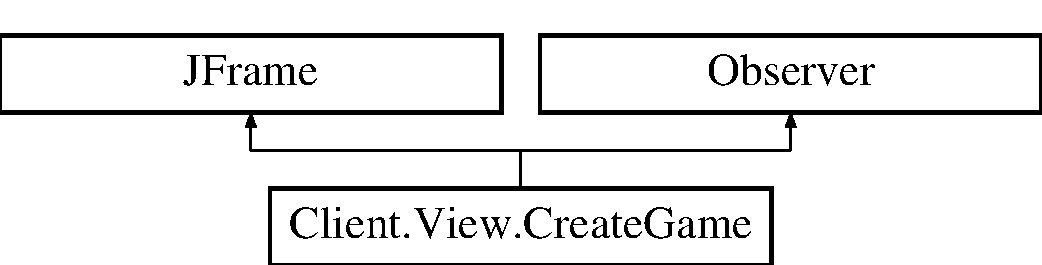
\includegraphics[height=2.000000cm]{a00035}
\end{center}
\end{figure}
\subsubsection*{Öffentliche Methoden}
\begin{DoxyCompactItemize}
\item 
\hyperlink{a00035_af35c00524077f6cda2d0c0397ce032a5}{Create\-Game} ()  throws I\-O\-Exception 
\item 
void \hyperlink{a00035_a0c95e9377fb0c48543c65d7c39c26fc1}{update} (Observable o, Object arg)
\end{DoxyCompactItemize}


\subsubsection{Ausführliche Beschreibung}
Es bietet alle Komponenten, um ein Regelwerk zu w�hlen, einen Spielnamen festzulegen und das Spiel durch ein Passwort zu sch�tzen. In der Spielerstellung wird ein Titelbild des ausgew�hlten Spiels und eine kurze Beschreibung angezeigt. �ber 'Leave' kehrt der Spieler in die \hyperlink{a00053}{Lobby} zur�ck und mit 'Create' wird das Spiel erstellt.

\begin{DoxyAuthor}{Autor}
M4nkey 
\end{DoxyAuthor}


\subsubsection{Beschreibung der Konstruktoren und Destruktoren}
\hypertarget{a00035_af35c00524077f6cda2d0c0397ce032a5}{\index{Client\-::\-View\-::\-Create\-Game@{Client\-::\-View\-::\-Create\-Game}!Create\-Game@{Create\-Game}}
\index{Create\-Game@{Create\-Game}!Client::View::CreateGame@{Client\-::\-View\-::\-Create\-Game}}
\paragraph[{Create\-Game}]{\setlength{\rightskip}{0pt plus 5cm}Client.\-View.\-Create\-Game.\-Create\-Game (
\begin{DoxyParamCaption}
{}
\end{DoxyParamCaption}
) throws I\-O\-Exception}}\label{a00035_af35c00524077f6cda2d0c0397ce032a5}


Erstellt das \hyperlink{a00035}{Create\-Game} Fenster. 


\begin{DoxyExceptions}{Ausnahmebehandlung}
{\em I\-O\-Exception} & \\
\hline
\end{DoxyExceptions}


\subsubsection{Dokumentation der Elementfunktionen}
\hypertarget{a00035_a0c95e9377fb0c48543c65d7c39c26fc1}{\index{Client\-::\-View\-::\-Create\-Game@{Client\-::\-View\-::\-Create\-Game}!update@{update}}
\index{update@{update}!Client::View::CreateGame@{Client\-::\-View\-::\-Create\-Game}}
\paragraph[{update}]{\setlength{\rightskip}{0pt plus 5cm}void Client.\-View.\-Create\-Game.\-update (
\begin{DoxyParamCaption}
\item[{Observable}]{o, }
\item[{Object}]{arg}
\end{DoxyParamCaption}
)}}\label{a00035_a0c95e9377fb0c48543c65d7c39c26fc1}


Wird durch notify() im \hyperlink{a00013}{Client\-Model} aufgerufen. 

Je nach dem in arg �bergebenen Befehl wird ein Update des Fensters ausgef�hrt oder eine Fehlermeldung angezeigt.


\begin{DoxyParams}{Parameter}
{\em o} & erwartet ein Objekt von der Klasse \hyperlink{a00013}{Client\-Model} \\
\hline
{\em arg} & erwartet\-: window\-Change\-Acknowledged, window\-Change\-Denied \\
\hline
\end{DoxyParams}

\hypertarget{a00036}{\subsection{Client.\-View.\-Discard\-Pile Klassenreferenz}
\label{a00036}\index{Client.\-View.\-Discard\-Pile@{Client.\-View.\-Discard\-Pile}}
}


\subsubsection{Ausführliche Beschreibung}
\begin{DoxyAuthor}{Autor}
m4nkey 
\end{DoxyAuthor}

\hypertarget{a00037}{\subsection{Client.\-View.\-Draw\-Deck Klassenreferenz}
\label{a00037}\index{Client.\-View.\-Draw\-Deck@{Client.\-View.\-Draw\-Deck}}
}


\subsubsection{Ausführliche Beschreibung}
\begin{DoxyAuthor}{Autor}
m4nkey 
\end{DoxyAuthor}

\hypertarget{a00038}{\subsection{Client.\-View.\-Game Klassenreferenz}
\label{a00038}\index{Client.\-View.\-Game@{Client.\-View.\-Game}}
}
Klassendiagramm für Client.\-View.\-Game\-:\begin{figure}[H]
\begin{center}
\leavevmode
\includegraphics[height=2.000000cm]{a00038}
\end{center}
\end{figure}
\subsubsection*{Öffentliche Methoden}
\begin{DoxyCompactItemize}
\item 
\hyperlink{a00038_afe6d788e3d6d0c2b8f052d966bf6cea1}{Game} ()  throws I\-O\-Exception 
\item 
void \hyperlink{a00038_af04de16e7780bba7e3acab2554390b80}{update} (Observable o, Object arg)
\end{DoxyCompactItemize}


\subsubsection{Ausführliche Beschreibung}
Au�erdem k�nnen �ber ein Dropdown-\/\-Men� �nderungen an Hintergrundbild und Kartenhintergr�nden vorgenommen werden. Schlie�en beendet das Spiel und der Spieler wird in die \hyperlink{a00053}{Lobby} zur�ckgeleitet.

\begin{DoxyAuthor}{Autor}
M4nkey 
\end{DoxyAuthor}


\subsubsection{Beschreibung der Konstruktoren und Destruktoren}
\hypertarget{a00038_afe6d788e3d6d0c2b8f052d966bf6cea1}{\index{Client\-::\-View\-::\-Game@{Client\-::\-View\-::\-Game}!Game@{Game}}
\index{Game@{Game}!Client::View::Game@{Client\-::\-View\-::\-Game}}
\paragraph[{Game}]{\setlength{\rightskip}{0pt plus 5cm}Client.\-View.\-Game.\-Game (
\begin{DoxyParamCaption}
{}
\end{DoxyParamCaption}
) throws I\-O\-Exception}}\label{a00038_afe6d788e3d6d0c2b8f052d966bf6cea1}


Erstellt das \hyperlink{a00038}{Game} Fenster. 


\begin{DoxyExceptions}{Ausnahmebehandlung}
{\em I\-O\-Exception} & \\
\hline
\end{DoxyExceptions}


\subsubsection{Dokumentation der Elementfunktionen}
\hypertarget{a00038_af04de16e7780bba7e3acab2554390b80}{\index{Client\-::\-View\-::\-Game@{Client\-::\-View\-::\-Game}!update@{update}}
\index{update@{update}!Client::View::Game@{Client\-::\-View\-::\-Game}}
\paragraph[{update}]{\setlength{\rightskip}{0pt plus 5cm}void Client.\-View.\-Game.\-update (
\begin{DoxyParamCaption}
\item[{Observable}]{o, }
\item[{Object}]{arg}
\end{DoxyParamCaption}
)}}\label{a00038_af04de16e7780bba7e3acab2554390b80}


Wird durch notify() im \hyperlink{a00013}{Client\-Model} aufgerufen. 

Je nach dem in arg �bergebenen Befehl wird ein Update des Fensters ausgef�hrt oder eine Fehlermeldung angezeigt.


\begin{DoxyParams}{Parameter}
{\em o} & erwartet ein Objekt von der Klasse \hyperlink{a00013}{Client\-Model} \\
\hline
{\em arg} & erwartet\-: chat\-Message, played\-Cards\-Update, other\-Data\-Update \\
\hline
\end{DoxyParams}

\hypertarget{a00039}{\subsection{Ruleset.\-Game\-Client\-Update Klassenreferenz}
\label{a00039}\index{Ruleset.\-Game\-Client\-Update@{Ruleset.\-Game\-Client\-Update}}
}
\subsubsection*{Öffentliche Methoden}
\begin{DoxyCompactItemize}
\item 
Array\-List$<$ \hyperlink{a00002}{Card} $>$ \hyperlink{a00039_a5169a0c2be5742c06b2a3b4723a345f4}{get\-Own\-Hand} ()
\item 
Map$<$ String, \hyperlink{a00002}{Card} $>$ \hyperlink{a00039_afdcfef45bd551867214d77414821d7e1}{get\-Played\-Cards} ()
\item 
\hyperlink{a00069}{Other\-Data} \hyperlink{a00039_a8c5d5e302f02decc32bfeaf896d13012}{get\-Own\-Data} ()
\item 
Array\-List$<$ \hyperlink{a00069}{Other\-Data} $>$ \hyperlink{a00039_a0662f7c0d8f8cdbb9916bf424aea1e18}{get\-Other\-Player\-Data} ()
\end{DoxyCompactItemize}


\subsubsection{Ausführliche Beschreibung}
Das w�ren seine Spielhand, der Ablagestapel sowie die Otherdata von allen Spielern. Bei Wizard enth�lt es auch die momentane Trumpfkarte. 

\subsubsection{Dokumentation der Elementfunktionen}
\hypertarget{a00039_a0662f7c0d8f8cdbb9916bf424aea1e18}{\index{Ruleset\-::\-Game\-Client\-Update@{Ruleset\-::\-Game\-Client\-Update}!get\-Other\-Player\-Data@{get\-Other\-Player\-Data}}
\index{get\-Other\-Player\-Data@{get\-Other\-Player\-Data}!Ruleset::GameClientUpdate@{Ruleset\-::\-Game\-Client\-Update}}
\paragraph[{get\-Other\-Player\-Data}]{\setlength{\rightskip}{0pt plus 5cm}Array\-List$<${\bf Other\-Data}$>$ Ruleset.\-Game\-Client\-Update.\-get\-Other\-Player\-Data (
\begin{DoxyParamCaption}
{}
\end{DoxyParamCaption}
)}}\label{a00039_a0662f7c0d8f8cdbb9916bf424aea1e18}


Holt die Spieldaten der anderen Spieler. 

\begin{DoxyReturn}{Rückgabe}
other\-Player\-Data Die Spieldaten der anderen Spieler 
\end{DoxyReturn}
\hypertarget{a00039_a8c5d5e302f02decc32bfeaf896d13012}{\index{Ruleset\-::\-Game\-Client\-Update@{Ruleset\-::\-Game\-Client\-Update}!get\-Own\-Data@{get\-Own\-Data}}
\index{get\-Own\-Data@{get\-Own\-Data}!Ruleset::GameClientUpdate@{Ruleset\-::\-Game\-Client\-Update}}
\paragraph[{get\-Own\-Data}]{\setlength{\rightskip}{0pt plus 5cm}{\bf Other\-Data} Ruleset.\-Game\-Client\-Update.\-get\-Own\-Data (
\begin{DoxyParamCaption}
{}
\end{DoxyParamCaption}
)}}\label{a00039_a8c5d5e302f02decc32bfeaf896d13012}


Holt die zus�tzlichen Spieldaten des Client. 

\begin{DoxyReturn}{Rückgabe}
own\-Data Die Spieldaten des Clients 
\end{DoxyReturn}
\hypertarget{a00039_a5169a0c2be5742c06b2a3b4723a345f4}{\index{Ruleset\-::\-Game\-Client\-Update@{Ruleset\-::\-Game\-Client\-Update}!get\-Own\-Hand@{get\-Own\-Hand}}
\index{get\-Own\-Hand@{get\-Own\-Hand}!Ruleset::GameClientUpdate@{Ruleset\-::\-Game\-Client\-Update}}
\paragraph[{get\-Own\-Hand}]{\setlength{\rightskip}{0pt plus 5cm}Array\-List$<${\bf Card}$>$ Ruleset.\-Game\-Client\-Update.\-get\-Own\-Hand (
\begin{DoxyParamCaption}
{}
\end{DoxyParamCaption}
)}}\label{a00039_a5169a0c2be5742c06b2a3b4723a345f4}


Holt die Karten die der Client auf der Hand hat. 

\begin{DoxyReturn}{Rückgabe}
own\-Hand Die Hand des Clients 
\end{DoxyReturn}
\hypertarget{a00039_afdcfef45bd551867214d77414821d7e1}{\index{Ruleset\-::\-Game\-Client\-Update@{Ruleset\-::\-Game\-Client\-Update}!get\-Played\-Cards@{get\-Played\-Cards}}
\index{get\-Played\-Cards@{get\-Played\-Cards}!Ruleset::GameClientUpdate@{Ruleset\-::\-Game\-Client\-Update}}
\paragraph[{get\-Played\-Cards}]{\setlength{\rightskip}{0pt plus 5cm}Map$<$String, {\bf Card}$>$ Ruleset.\-Game\-Client\-Update.\-get\-Played\-Cards (
\begin{DoxyParamCaption}
{}
\end{DoxyParamCaption}
)}}\label{a00039_afdcfef45bd551867214d77414821d7e1}


Holt die gespielten Karten auf dem Ablagestapel. 

\begin{DoxyReturn}{Rückgabe}
discard\-Pile Die gespielten Karten 
\end{DoxyReturn}

\hypertarget{a00040}{\subsection{Com\-Start\-Game Klassenreferenz}
\label{a00040}\index{Com\-Start\-Game@{Com\-Start\-Game}}
}


Abgeleitet von \hyperlink{a00037}{Com\-Object} und Serializable.

\subsubsection*{Öffentliche Methoden}
\begin{DoxyCompactItemize}
\item 
\hypertarget{a00040_a96b5e8f54fa85641a2f50624f4939202}{\hyperlink{a00040_a96b5e8f54fa85641a2f50624f4939202}{Com\-Start\-Game} ()}\label{a00040_a96b5e8f54fa85641a2f50624f4939202}

\item 
void \hyperlink{a00040_a758d7005755a181717f238f714d87dd2}{process} (\hyperlink{a00003}{Client\-Model} model)
\item 
void \hyperlink{a00040_ac67b5ce3ec03d48ef1e6caad6e49c902}{process} (\hyperlink{a00076}{Player} player, \hyperlink{a00077}{Server} server)
\end{DoxyCompactItemize}


\subsubsection{Ausführliche Beschreibung}
Diese Klasse ist ein spezielles Kommunikations-\/\-Objekt. Sie wird versendet, wenn ein Spiel gestartet werden soll. 

\subsubsection{Dokumentation der Elementfunktionen}
\hypertarget{a00040_a758d7005755a181717f238f714d87dd2}{\index{Com\-Objects\-::\-Com\-Start\-Game@{Com\-Objects\-::\-Com\-Start\-Game}!process@{process}}
\index{process@{process}!ComObjects::ComStartGame@{Com\-Objects\-::\-Com\-Start\-Game}}
\paragraph[{process}]{\setlength{\rightskip}{0pt plus 5cm}void process (
\begin{DoxyParamCaption}
\item[{{\bf Client\-Model}}]{model}
\end{DoxyParamCaption}
)}}\label{a00040_a758d7005755a181717f238f714d87dd2}


Diese Methode ist noetig, damit der Client\-Listener\-Thread entscheiden kann welche Message das Object enthaelt und wie diese verarbeitet werden soll. 


\begin{DoxyParams}{Parameter}
{\em model} & ist das Client\-Model, welches übergeben wird, damit die ueberladene Methode richtig gewaehlt wird. \\
\hline
\end{DoxyParams}


Implementiert \hyperlink{a00037_a758d7005755a181717f238f714d87dd2}{Com\-Object}.

\hypertarget{a00040_ac67b5ce3ec03d48ef1e6caad6e49c902}{\index{Com\-Objects\-::\-Com\-Start\-Game@{Com\-Objects\-::\-Com\-Start\-Game}!process@{process}}
\index{process@{process}!ComObjects::ComStartGame@{Com\-Objects\-::\-Com\-Start\-Game}}
\paragraph[{process}]{\setlength{\rightskip}{0pt plus 5cm}void process (
\begin{DoxyParamCaption}
\item[{{\bf Player}}]{player, }
\item[{{\bf Server}}]{server}
\end{DoxyParamCaption}
)}}\label{a00040_ac67b5ce3ec03d48ef1e6caad6e49c902}


Diese Methode ist noetig, damit der Thread Player entscheiden kann welche Message das Object enthaelt und wie diese verarbeitet werden soll. 


\begin{DoxyParams}{Parameter}
{\em player} & Der Client welcher den Aufruf startet. \\
\hline
{\em server} & Der Server an den sich das Com\-Objekt weitergibt. \\
\hline
\end{DoxyParams}


Implementiert \hyperlink{a00037_ac67b5ce3ec03d48ef1e6caad6e49c902}{Com\-Object}.


\hypertarget{a00041}{\subsection{Client.\-View.\-Game\-Panel Klassenreferenz}
\label{a00041}\index{Client.\-View.\-Game\-Panel@{Client.\-View.\-Game\-Panel}}
}
Klassendiagramm für Client.\-View.\-Game\-Panel\-:\begin{figure}[H]
\begin{center}
\leavevmode
\includegraphics[height=2.000000cm]{a00041}
\end{center}
\end{figure}


\subsubsection{Ausführliche Beschreibung}
Es besteht aus veschiedenen Panelobjekten, welche je nach Regelwerk auf das Spielfeld gezeichnet werden. Dazu geh�ren die eigenen Karten, eventuell ausgew�hlte Karten, ein Textfeld z.\-B. zur Anzeige der Anzahl der restlichen Karten der Mitspieler und den Ablagestapel (/\-L194/). Nach jeder Runde wird der Punktestand aktualisiert.

\begin{DoxyAuthor}{Autor}
m4nkey 
\end{DoxyAuthor}

\hypertarget{a00042}{\subsection{Com\-Warning Klassenreferenz}
\label{a00042}\index{Com\-Warning@{Com\-Warning}}
}


Abgeleitet von \hyperlink{a00037}{Com\-Object} und Serializable.

\subsubsection*{Öffentliche Methoden}
\begin{DoxyCompactItemize}
\item 
\hyperlink{a00042_a5c697b925b40d1ec204a2d45c0bccccb}{Com\-Warning} (String warning)
\item 
String \hyperlink{a00042_a871f3f6b982d1e3b4468a95f99a083e1}{get\-Warning} ()
\item 
void \hyperlink{a00042_a758d7005755a181717f238f714d87dd2}{process} (\hyperlink{a00003}{Client\-Model} model)
\item 
void \hyperlink{a00042_ac67b5ce3ec03d48ef1e6caad6e49c902}{process} (\hyperlink{a00076}{Player} player, \hyperlink{a00077}{Server} server)
\end{DoxyCompactItemize}
\subsubsection*{Private Attribute}
\begin{DoxyCompactItemize}
\item 
\hypertarget{a00042_a393c8163a2f6f4a86dbd8b8793d341f3}{String {\bfseries warning}}\label{a00042_a393c8163a2f6f4a86dbd8b8793d341f3}

\end{DoxyCompactItemize}


\subsubsection{Ausführliche Beschreibung}
Diese Klasse ist ein spezielles Kommunikations-\/\-Objekt. Sie soll dem Spieler eine Mitteilung senden und so ueber ein Fehlerevent informieren. 

\subsubsection{Beschreibung der Konstruktoren und Destruktoren}
\hypertarget{a00042_a5c697b925b40d1ec204a2d45c0bccccb}{\index{Com\-Objects\-::\-Com\-Warning@{Com\-Objects\-::\-Com\-Warning}!Com\-Warning@{Com\-Warning}}
\index{Com\-Warning@{Com\-Warning}!ComObjects::ComWarning@{Com\-Objects\-::\-Com\-Warning}}
\paragraph[{Com\-Warning}]{\setlength{\rightskip}{0pt plus 5cm}{\bf Com\-Warning} (
\begin{DoxyParamCaption}
\item[{String}]{warning}
\end{DoxyParamCaption}
)}}\label{a00042_a5c697b925b40d1ec204a2d45c0bccccb}


Dies ist der Konstruktor einer neuen Com\-Warning-\/\-Nachricht. 

Er enthaelt eine Warnung an den Spieler, wenn ein Fehler passiert. 
\begin{DoxyParams}{Parameter}
{\em warning} & ist die Warnung, die der Spieler erhaelt. \\
\hline
\end{DoxyParams}


\subsubsection{Dokumentation der Elementfunktionen}
\hypertarget{a00042_a871f3f6b982d1e3b4468a95f99a083e1}{\index{Com\-Objects\-::\-Com\-Warning@{Com\-Objects\-::\-Com\-Warning}!get\-Warning@{get\-Warning}}
\index{get\-Warning@{get\-Warning}!ComObjects::ComWarning@{Com\-Objects\-::\-Com\-Warning}}
\paragraph[{get\-Warning}]{\setlength{\rightskip}{0pt plus 5cm}String get\-Warning (
\begin{DoxyParamCaption}
{}
\end{DoxyParamCaption}
)}}\label{a00042_a871f3f6b982d1e3b4468a95f99a083e1}


Diese Methode gibt die Nachricht zurueck, die dem Spieler den Fehler mitteilt. 

\begin{DoxyReturn}{Rückgabe}
die Warnnachricht. 
\end{DoxyReturn}
\hypertarget{a00042_a758d7005755a181717f238f714d87dd2}{\index{Com\-Objects\-::\-Com\-Warning@{Com\-Objects\-::\-Com\-Warning}!process@{process}}
\index{process@{process}!ComObjects::ComWarning@{Com\-Objects\-::\-Com\-Warning}}
\paragraph[{process}]{\setlength{\rightskip}{0pt plus 5cm}void process (
\begin{DoxyParamCaption}
\item[{{\bf Client\-Model}}]{model}
\end{DoxyParamCaption}
)}}\label{a00042_a758d7005755a181717f238f714d87dd2}


Diese Methode ist noetig, damit der Client\-Listener\-Thread entscheiden kann welche Message das Object enthaelt und wie diese verarbeitet werden soll. 


\begin{DoxyParams}{Parameter}
{\em model} & ist das Client\-Model, welches übergeben wird, damit die ueberladene Methode richtig gewaehlt wird. \\
\hline
\end{DoxyParams}


Implementiert \hyperlink{a00037_a758d7005755a181717f238f714d87dd2}{Com\-Object}.

\hypertarget{a00042_ac67b5ce3ec03d48ef1e6caad6e49c902}{\index{Com\-Objects\-::\-Com\-Warning@{Com\-Objects\-::\-Com\-Warning}!process@{process}}
\index{process@{process}!ComObjects::ComWarning@{Com\-Objects\-::\-Com\-Warning}}
\paragraph[{process}]{\setlength{\rightskip}{0pt plus 5cm}void process (
\begin{DoxyParamCaption}
\item[{{\bf Player}}]{player, }
\item[{{\bf Server}}]{server}
\end{DoxyParamCaption}
)}}\label{a00042_ac67b5ce3ec03d48ef1e6caad6e49c902}


Diese Methode ist noetig, damit der Thread Player entscheiden kann welche Message das Object enthaelt und wie diese verarbeitet werden soll. 


\begin{DoxyParams}{Parameter}
{\em player} & Der Client welcher den Aufruf startet. \\
\hline
{\em server} & Der Server an den sich das Com\-Objekt weitergibt. \\
\hline
\end{DoxyParams}


Implementiert \hyperlink{a00037_ac67b5ce3ec03d48ef1e6caad6e49c902}{Com\-Object}.


\hypertarget{a00043}{\subsection{Server.\-Game\-Server Klassenreferenz}
\label{a00043}\index{Server.\-Game\-Server@{Server.\-Game\-Server}}
}
Klassendiagramm für Server.\-Game\-Server\-:\begin{figure}[H]
\begin{center}
\leavevmode
\includegraphics[height=2.000000cm]{a00043}
\end{center}
\end{figure}
\subsubsection*{Öffentliche Methoden}
\begin{DoxyCompactItemize}
\item 
\hyperlink{a00043_a6db144e60c51cb6ee80f448104127aed}{Game\-Server} (\hyperlink{a00054}{Lobby\-Server} server, \hyperlink{a00073}{Player} game\-Master, String Game\-Name, \hyperlink{a00076}{Ruleset\-Type} ruleset, String password, boolean has\-Password)
\item 
synchronized void \hyperlink{a00043_a942046c7512e4fead06f7df12faa119f}{add\-Player} (\hyperlink{a00073}{Player} player)
\item 
synchronized void \hyperlink{a00043_afc6cc835652484da1b7b1fda6071ea0b}{remove\-Player} (\hyperlink{a00073}{Player} player)
\item 
void \hyperlink{a00043_aae9201e5827933e23b078bc7eaf2aee3}{receive\-Message} (\hyperlink{a00073}{Player} player, Com\-Kick\-Player\-Request kick\-Player)
\item 
void \hyperlink{a00043_a7112c8a4b95e71c42a207b844f447305}{receive\-Message} (\hyperlink{a00073}{Player} player, Com\-Chat\-Message chat)
\item 
void \hyperlink{a00043_a9fd05e79a3ae006b056cb27199ee7aeb}{receive\-Message} (\hyperlink{a00073}{Player} player, Com\-Client\-Leave leave)
\item 
void \hyperlink{a00043_af3affa434fc5afd574d4fa74060ac9c7}{receive\-Message} (\hyperlink{a00073}{Player} player, Com\-Client\-Quit quit)
\item 
void \hyperlink{a00043_accca048ccec6323df6d3262f96d98723}{receive\-Message} (\hyperlink{a00073}{Player} player, Com\-Start\-Game start)
\item 
void \hyperlink{a00043_accad199750d7c6577b2d096483ce6e9d}{receive\-Message} (\hyperlink{a00073}{Player} player, Com\-Ruleset ruleset)
\item 
Com\-Init\-Game\-Lobby \hyperlink{a00043_a4e2b83f3466ec6c9cbe0a24a30587333}{init\-Lobby} ()
\end{DoxyCompactItemize}


\subsubsection{Ausführliche Beschreibung}
Sie verwaltet die Kommunikation zwischen den Clients w�hrend eines Spieles. Die Game\-Server-\/\-Klasse erbt Methoden zur Kommunikation vom \hyperlink{a00078}{Server}. Der \hyperlink{a00043}{Game\-Server} tauscht Nachrichten zwischen Ruleset und \hyperlink{a00073}{Player} aus, um so den Spielablauf zu koordinieren. \begin{DoxyAuthor}{Autor}
Viktoria 
\end{DoxyAuthor}


\subsubsection{Beschreibung der Konstruktoren und Destruktoren}
\hypertarget{a00043_a6db144e60c51cb6ee80f448104127aed}{\index{Server\-::\-Game\-Server@{Server\-::\-Game\-Server}!Game\-Server@{Game\-Server}}
\index{Game\-Server@{Game\-Server}!Server::GameServer@{Server\-::\-Game\-Server}}
\paragraph[{Game\-Server}]{\setlength{\rightskip}{0pt plus 5cm}Server.\-Game\-Server.\-Game\-Server (
\begin{DoxyParamCaption}
\item[{{\bf Lobby\-Server}}]{server, }
\item[{{\bf Player}}]{game\-Master, }
\item[{String}]{Game\-Name, }
\item[{{\bf Ruleset\-Type}}]{ruleset, }
\item[{String}]{password, }
\item[{boolean}]{has\-Password}
\end{DoxyParamCaption}
)}}\label{a00043_a6db144e60c51cb6ee80f448104127aed}


Konstruktor des Game\-Servers. 

Setzt die Attribute lobby\-Server, name, password, has\-Pasword und ruleset\-Type auf die �bergebenen Werte. Setzt den game\-Master\-Name auf den Namen des game\-Master und f�gt den game\-Master dem Set an Spielern hinzu. Bestimmt mithilfe des Enums Ruleset\-Type das Ruleset und erstellt es. Setzt current\-Players auf eins und max\-Players je nach Ruleset. 
\begin{DoxyParams}{Parameter}
{\em server} & ist der \hyperlink{a00054}{Lobby\-Server} der den \hyperlink{a00043}{Game\-Server} erstellt hat. \\
\hline
{\em game\-Master} & ist der Name des Spielleiters \\
\hline
{\em Game\-Name} & ist der Name des Spiels \\
\hline
{\em ruleset} & gibt an, welches Ruleset verwendet wird \\
\hline
{\em password} & speichert das Passwort des Spiels \\
\hline
{\em has\-Password} & gibt an,ob das Spiel ein Passwort hat \\
\hline
\end{DoxyParams}


\subsubsection{Dokumentation der Elementfunktionen}
\hypertarget{a00043_a942046c7512e4fead06f7df12faa119f}{\index{Server\-::\-Game\-Server@{Server\-::\-Game\-Server}!add\-Player@{add\-Player}}
\index{add\-Player@{add\-Player}!Server::GameServer@{Server\-::\-Game\-Server}}
\paragraph[{add\-Player}]{\setlength{\rightskip}{0pt plus 5cm}synchronized void Server.\-Game\-Server.\-add\-Player (
\begin{DoxyParamCaption}
\item[{{\bf Player}}]{player}
\end{DoxyParamCaption}
)}}\label{a00043_a942046c7512e4fead06f7df12faa119f}


Diese Methode wird vom abstrakten \hyperlink{a00078}{Server} vererbt. 

Zus�tzlich wird die Zahl der current\-Players um eins Erh�ht. 
\begin{DoxyParams}{Parameter}
{\em player} & ist der \hyperlink{a00073}{Player}, der hinzugefo�gt wird \\
\hline
\end{DoxyParams}
\hypertarget{a00043_a4e2b83f3466ec6c9cbe0a24a30587333}{\index{Server\-::\-Game\-Server@{Server\-::\-Game\-Server}!init\-Lobby@{init\-Lobby}}
\index{init\-Lobby@{init\-Lobby}!Server::GameServer@{Server\-::\-Game\-Server}}
\paragraph[{init\-Lobby}]{\setlength{\rightskip}{0pt plus 5cm}Com\-Init\-Game\-Lobby Server.\-Game\-Server.\-init\-Lobby (
\begin{DoxyParamCaption}
{}
\end{DoxyParamCaption}
)}}\label{a00043_a4e2b83f3466ec6c9cbe0a24a30587333}


Baut ein neues Com\-Init\-Game\-Lobby Objekt und gibt es zur�ck. 

\begin{DoxyReturn}{Rückgabe}
Gibt das Com\-Init\-Game\-Lobby Objekt zur�ck 
\end{DoxyReturn}
\hypertarget{a00043_aae9201e5827933e23b078bc7eaf2aee3}{\index{Server\-::\-Game\-Server@{Server\-::\-Game\-Server}!receive\-Message@{receive\-Message}}
\index{receive\-Message@{receive\-Message}!Server::GameServer@{Server\-::\-Game\-Server}}
\paragraph[{receive\-Message}]{\setlength{\rightskip}{0pt plus 5cm}void Server.\-Game\-Server.\-receive\-Message (
\begin{DoxyParamCaption}
\item[{{\bf Player}}]{player, }
\item[{Com\-Kick\-Player\-Request}]{kick\-Player}
\end{DoxyParamCaption}
)}}\label{a00043_aae9201e5827933e23b078bc7eaf2aee3}


Diese Methode ist dafur zust�ndig zu ermitteln, was passiert wenn ein Spieler aus der Game\-Lobby geworfen wird. 

Der \hyperlink{a00073}{Player} wird durch Aufruf von change\-Server an die Lobby zur�ckgegeben. An diesen Spieler wird ein Com\-Warning und ein Com\-Init\-Lobby geschickt. Danach wird ein Com\-Update\-Playerlist Objekt mit broadcast an alle Client im Spiel verschickt. 
\begin{DoxyParams}{Parameter}
{\em player} & ist der Threat der die Nachricht erhalten hat \\
\hline
{\em kicked} & ist das Com\-Object, das verarbeitet wird \\
\hline
\end{DoxyParams}
\hypertarget{a00043_a7112c8a4b95e71c42a207b844f447305}{\index{Server\-::\-Game\-Server@{Server\-::\-Game\-Server}!receive\-Message@{receive\-Message}}
\index{receive\-Message@{receive\-Message}!Server::GameServer@{Server\-::\-Game\-Server}}
\paragraph[{receive\-Message}]{\setlength{\rightskip}{0pt plus 5cm}void Server.\-Game\-Server.\-receive\-Message (
\begin{DoxyParamCaption}
\item[{{\bf Player}}]{player, }
\item[{Com\-Chat\-Message}]{chat}
\end{DoxyParamCaption}
)}}\label{a00043_a7112c8a4b95e71c42a207b844f447305}


Diese Methode ist dafur zust�ndig eine Chatnachricht an alle Clients im Spiel zu verschicken. 

Daf�r wird die Com\-Chat\-Message mit broadcast an alle Spieler im player\-Set verteilt. 
\begin{DoxyParams}{Parameter}
{\em player} & ist der Threat der die Nachricht erhalten hat \\
\hline
{\em chat} & ist das Com\-Object, das die Chatnachricht enth�lt \\
\hline
\end{DoxyParams}
\hypertarget{a00043_a9fd05e79a3ae006b056cb27199ee7aeb}{\index{Server\-::\-Game\-Server@{Server\-::\-Game\-Server}!receive\-Message@{receive\-Message}}
\index{receive\-Message@{receive\-Message}!Server::GameServer@{Server\-::\-Game\-Server}}
\paragraph[{receive\-Message}]{\setlength{\rightskip}{0pt plus 5cm}void Server.\-Game\-Server.\-receive\-Message (
\begin{DoxyParamCaption}
\item[{{\bf Player}}]{player, }
\item[{Com\-Client\-Leave}]{leave}
\end{DoxyParamCaption}
)}}\label{a00043_a9fd05e79a3ae006b056cb27199ee7aeb}


Diese Methode gibt einen \hyperlink{a00073}{Player}, der die Game\-Lobby verlassen will, durch Aufruf von change\-Server an die Server\-Lobby zur�ck und schickt ihm ein Com\-Init\-Lobby. 

Danach wird ein Com\-Update\-Playerlist Objekt mit broadcast an alle Clients im Spiel verschickt. 
\begin{DoxyParams}{Parameter}
{\em player} & ist der Threat der die Nachricht erhalten hat \\
\hline
{\em leave} & ist das Com\-Object, welches angibt, dass der Spieler in die Lobby zur�ckkehrt \\
\hline
\end{DoxyParams}
\hypertarget{a00043_af3affa434fc5afd574d4fa74060ac9c7}{\index{Server\-::\-Game\-Server@{Server\-::\-Game\-Server}!receive\-Message@{receive\-Message}}
\index{receive\-Message@{receive\-Message}!Server::GameServer@{Server\-::\-Game\-Server}}
\paragraph[{receive\-Message}]{\setlength{\rightskip}{0pt plus 5cm}void Server.\-Game\-Server.\-receive\-Message (
\begin{DoxyParamCaption}
\item[{{\bf Player}}]{player, }
\item[{Com\-Client\-Quit}]{quit}
\end{DoxyParamCaption}
)}}\label{a00043_af3affa434fc5afd574d4fa74060ac9c7}


Diese Methode behandelt den Fall, dass ein Spieler das laufende Spiel verl�sst. 

Sie gibt einen \hyperlink{a00073}{Player}, der das Spiel verlassen will, Aufruf von change\-Server an die Server\-Lobby zur�ck und schickt ihm ein Com\-Init\-Lobby. Alle Spieler, die sich im Spiel befinden bekommen ein Com\-Warning und ein Com\-Init\-Lobby und werden durch Aufruf von change\-Server an die Lobby zur�ckgegeben. Das Spiel wird aufgel�st. 
\begin{DoxyParams}{Parameter}
{\em player} & ist der Threat der die Nachricht erhalten hat \\
\hline
{\em quit} & ist das Com\-Object, welches angibt, dass der Spieler das Spiel verl�sst \\
\hline
\end{DoxyParams}
\hypertarget{a00043_accca048ccec6323df6d3262f96d98723}{\index{Server\-::\-Game\-Server@{Server\-::\-Game\-Server}!receive\-Message@{receive\-Message}}
\index{receive\-Message@{receive\-Message}!Server::GameServer@{Server\-::\-Game\-Server}}
\paragraph[{receive\-Message}]{\setlength{\rightskip}{0pt plus 5cm}void Server.\-Game\-Server.\-receive\-Message (
\begin{DoxyParamCaption}
\item[{{\bf Player}}]{player, }
\item[{Com\-Start\-Game}]{start}
\end{DoxyParamCaption}
)}}\label{a00043_accca048ccec6323df6d3262f96d98723}


Diese Methode sagt dem Ruleset, dass ein neues Spiel gestartet werden soll. 


\begin{DoxyParams}{Parameter}
{\em player} & ist der Threat der die Nachricht erhalten hat \\
\hline
{\em start} & ist das Com\-Object, dass angibt, dass das Spiel gestartet werden soll \\
\hline
\end{DoxyParams}
\hypertarget{a00043_accad199750d7c6577b2d096483ce6e9d}{\index{Server\-::\-Game\-Server@{Server\-::\-Game\-Server}!receive\-Message@{receive\-Message}}
\index{receive\-Message@{receive\-Message}!Server::GameServer@{Server\-::\-Game\-Server}}
\paragraph[{receive\-Message}]{\setlength{\rightskip}{0pt plus 5cm}void Server.\-Game\-Server.\-receive\-Message (
\begin{DoxyParamCaption}
\item[{{\bf Player}}]{player, }
\item[{Com\-Ruleset}]{ruleset}
\end{DoxyParamCaption}
)}}\label{a00043_accad199750d7c6577b2d096483ce6e9d}


Diese Methode gibt das erhaltene Com\-Ruleset durch einen Aufruf von resolve\-Message an das Ruleset weiter. 


\begin{DoxyParams}{Parameter}
{\em player} & ist der Threat der die Nachricht erhalten hat \\
\hline
{\em ruleset} & ist das Com\-Object, das zeigt, dass das Object vom Ruleset bearbeitet werden muss \\
\hline
\end{DoxyParams}
\hypertarget{a00043_afc6cc835652484da1b7b1fda6071ea0b}{\index{Server\-::\-Game\-Server@{Server\-::\-Game\-Server}!remove\-Player@{remove\-Player}}
\index{remove\-Player@{remove\-Player}!Server::GameServer@{Server\-::\-Game\-Server}}
\paragraph[{remove\-Player}]{\setlength{\rightskip}{0pt plus 5cm}synchronized void Server.\-Game\-Server.\-remove\-Player (
\begin{DoxyParamCaption}
\item[{{\bf Player}}]{player}
\end{DoxyParamCaption}
)}}\label{a00043_afc6cc835652484da1b7b1fda6071ea0b}


Diese Methode wird vom abstrakten \hyperlink{a00078}{Server} vererbt. 

Zus�tzlich wird die Zahl der current\-Players um eins Verringert. 
\begin{DoxyParams}{Parameter}
{\em player} & ist der \hyperlink{a00073}{Player}, der entfernt wird \\
\hline
\end{DoxyParams}

\hypertarget{a00044}{\subsection{Server.\-Game\-Server\-Representation Klassenreferenz}
\label{a00044}\index{Server.\-Game\-Server\-Representation@{Server.\-Game\-Server\-Representation}}
}
\subsubsection*{Öffentliche Methoden}
\begin{DoxyCompactItemize}
\item 
\hyperlink{a00044_afabe1ef940660d5ccde15467933d0ad0}{Game\-Server\-Representation} (String game\-Master, String game\-Name, int max, int current, \hyperlink{a00076}{Ruleset\-Type} type, boolean password)
\end{DoxyCompactItemize}


\subsubsection{Ausführliche Beschreibung}
Sie wird dem Com\-Objekt Com\-Lobby\-Update\-Game\-List angehängt, um die Spielliste in der Game\-Lobby aktualisieren zu können \begin{DoxyAuthor}{Autor}
Viktoria 
\end{DoxyAuthor}


\subsubsection{Beschreibung der Konstruktoren und Destruktoren}
\hypertarget{a00044_afabe1ef940660d5ccde15467933d0ad0}{\index{Server\-::\-Game\-Server\-Representation@{Server\-::\-Game\-Server\-Representation}!Game\-Server\-Representation@{Game\-Server\-Representation}}
\index{Game\-Server\-Representation@{Game\-Server\-Representation}!Server::GameServerRepresentation@{Server\-::\-Game\-Server\-Representation}}
\paragraph[{Game\-Server\-Representation}]{\setlength{\rightskip}{0pt plus 5cm}Server.\-Game\-Server\-Representation.\-Game\-Server\-Representation (
\begin{DoxyParamCaption}
\item[{String}]{game\-Master, }
\item[{String}]{game\-Name, }
\item[{int}]{max, }
\item[{int}]{current, }
\item[{{\bf Ruleset\-Type}}]{type, }
\item[{boolean}]{password}
\end{DoxyParamCaption}
)}}\label{a00044_afabe1ef940660d5ccde15467933d0ad0}


Der Konstruktor der Klasse \hyperlink{a00044}{Game\-Server\-Representation} initialisiert die Attribute mit den vom \hyperlink{a00043}{Game\-Server} übergebenen Werten. 


\begin{DoxyParams}{Parameter}
{\em game\-Master} & der Name des Spielleiters \\
\hline
{\em game\-Name} & der Name des Spiels \\
\hline
{\em max} & Maximal mögliche Anzahl teilnehmender Spieler \\
\hline
{\em current} & Anzahl momentaner Spieler \\
\hline
{\em type} & Welches Ruleset verwendet wird \\
\hline
{\em password} & ob das Spiel ein Passwort hat \\
\hline
\end{DoxyParams}

\hypertarget{a00045}{\subsection{Ruleset.\-Game\-State Klassenreferenz}
\label{a00045}\index{Ruleset.\-Game\-State@{Ruleset.\-Game\-State}}
}
\subsubsection*{Öffentliche Methoden}
\begin{DoxyCompactItemize}
\item 
void \hyperlink{a00045_adcdd80db7006a129d2681ef2156d8030}{set\-Current\-Player} (\hyperlink{a00074}{Player\-State} player)
\item 
\hyperlink{a00074}{Player\-State} \hyperlink{a00045_a940b04c3b7b3e4b2a407b77fa40cce33}{get\-Current\-Player} ()
\item 
Array\-List$<$ \hyperlink{a00002}{Card} $>$ \hyperlink{a00045_acbb1847c191f8642f77c72b971663602}{get\-Cards\-Left\-In\-Deck} ()
\item 
Map$<$ String, \hyperlink{a00002}{Card} $>$ \hyperlink{a00045_a1c3dd6d0e4fd89dd49eb5073c1e06234}{get\-Played\-Cards} ()
\item 
\hyperlink{a00074}{Player\-State} \hyperlink{a00045_aa087b905d7f5b7ac4f7f3356b7d0f06d}{get\-Player} (String name)
\item 
void \hyperlink{a00045_a6cbf9650695639cdbccfc520cc9b112f}{set\-Trump\-Card} (\hyperlink{a00002}{Card} trump\-Card)
\item 
\hyperlink{a00002}{Card} \hyperlink{a00045_a263d6b7805c19249a3a1243379480e87}{get\-Trump\-Card} ()
\item 
int \hyperlink{a00045_afef5de42e97641f5f4f46c2995697502}{get\-Number\-Of\-Played\-Cards} ()
\item 
boolean \hyperlink{a00045_a53e85a9b7f4fe195604de0f1e8a59550}{play\-Card} (\hyperlink{a00002}{Card} card)
\end{DoxyCompactItemize}


\subsubsection{Ausführliche Beschreibung}
Es enth�lt die einzelnen Player\-States, sowie Informationen zum Ablage-\/, Aufnahmestapel, Rundenanzahl, den momentan aktiven Spieler sowie \hyperlink{a00042}{Game\-Phase}. 

\subsubsection{Dokumentation der Elementfunktionen}
\hypertarget{a00045_acbb1847c191f8642f77c72b971663602}{\index{Ruleset\-::\-Game\-State@{Ruleset\-::\-Game\-State}!get\-Cards\-Left\-In\-Deck@{get\-Cards\-Left\-In\-Deck}}
\index{get\-Cards\-Left\-In\-Deck@{get\-Cards\-Left\-In\-Deck}!Ruleset::GameState@{Ruleset\-::\-Game\-State}}
\paragraph[{get\-Cards\-Left\-In\-Deck}]{\setlength{\rightskip}{0pt plus 5cm}Array\-List$<${\bf Card}$>$ Ruleset.\-Game\-State.\-get\-Cards\-Left\-In\-Deck (
\begin{DoxyParamCaption}
{}
\end{DoxyParamCaption}
)}}\label{a00045_acbb1847c191f8642f77c72b971663602}


Holt die Karten die noch im Aufnahmestapel sind. 

\begin{DoxyReturn}{Rückgabe}
cards\-Left\-In\-Deck Holt die Karten die noch im Aufnahmestapel sind 
\end{DoxyReturn}
\hypertarget{a00045_a940b04c3b7b3e4b2a407b77fa40cce33}{\index{Ruleset\-::\-Game\-State@{Ruleset\-::\-Game\-State}!get\-Current\-Player@{get\-Current\-Player}}
\index{get\-Current\-Player@{get\-Current\-Player}!Ruleset::GameState@{Ruleset\-::\-Game\-State}}
\paragraph[{get\-Current\-Player}]{\setlength{\rightskip}{0pt plus 5cm}{\bf Player\-State} Ruleset.\-Game\-State.\-get\-Current\-Player (
\begin{DoxyParamCaption}
{}
\end{DoxyParamCaption}
)}}\label{a00045_a940b04c3b7b3e4b2a407b77fa40cce33}


Holt den Spieler der momentan am Zug ist. 

\begin{DoxyReturn}{Rückgabe}
current\-Player Der Spielzustand des Spielers der grad am Zug ist 
\end{DoxyReturn}
\hypertarget{a00045_afef5de42e97641f5f4f46c2995697502}{\index{Ruleset\-::\-Game\-State@{Ruleset\-::\-Game\-State}!get\-Number\-Of\-Played\-Cards@{get\-Number\-Of\-Played\-Cards}}
\index{get\-Number\-Of\-Played\-Cards@{get\-Number\-Of\-Played\-Cards}!Ruleset::GameState@{Ruleset\-::\-Game\-State}}
\paragraph[{get\-Number\-Of\-Played\-Cards}]{\setlength{\rightskip}{0pt plus 5cm}int Ruleset.\-Game\-State.\-get\-Number\-Of\-Played\-Cards (
\begin{DoxyParamCaption}
{}
\end{DoxyParamCaption}
)}}\label{a00045_afef5de42e97641f5f4f46c2995697502}


Holt die Anzahl der gespielten Karten. 

\begin{DoxyReturn}{Rückgabe}
Die Anzahl der gespielten Karten 
\end{DoxyReturn}
\hypertarget{a00045_a1c3dd6d0e4fd89dd49eb5073c1e06234}{\index{Ruleset\-::\-Game\-State@{Ruleset\-::\-Game\-State}!get\-Played\-Cards@{get\-Played\-Cards}}
\index{get\-Played\-Cards@{get\-Played\-Cards}!Ruleset::GameState@{Ruleset\-::\-Game\-State}}
\paragraph[{get\-Played\-Cards}]{\setlength{\rightskip}{0pt plus 5cm}Map$<$String,{\bf Card}$>$ Ruleset.\-Game\-State.\-get\-Played\-Cards (
\begin{DoxyParamCaption}
{}
\end{DoxyParamCaption}
)}}\label{a00045_a1c3dd6d0e4fd89dd49eb5073c1e06234}


Holt die gespielten Karten im Ablagestapel. 

\begin{DoxyReturn}{Rückgabe}


discard\-Pile Die gespielten Karten 
\end{DoxyReturn}
\hypertarget{a00045_aa087b905d7f5b7ac4f7f3356b7d0f06d}{\index{Ruleset\-::\-Game\-State@{Ruleset\-::\-Game\-State}!get\-Player@{get\-Player}}
\index{get\-Player@{get\-Player}!Ruleset::GameState@{Ruleset\-::\-Game\-State}}
\paragraph[{get\-Player}]{\setlength{\rightskip}{0pt plus 5cm}{\bf Player\-State} Ruleset.\-Game\-State.\-get\-Player (
\begin{DoxyParamCaption}
\item[{String}]{name}
\end{DoxyParamCaption}
)}}\label{a00045_aa087b905d7f5b7ac4f7f3356b7d0f06d}


Holt einen bestimmten Spieler. 


\begin{DoxyParams}{Parameter}
{\em name} & Der Name des Spielers \\
\hline
\end{DoxyParams}
\begin{DoxyReturn}{Rückgabe}
player Der Spielzustand des Spielers 
\end{DoxyReturn}
\hypertarget{a00045_a263d6b7805c19249a3a1243379480e87}{\index{Ruleset\-::\-Game\-State@{Ruleset\-::\-Game\-State}!get\-Trump\-Card@{get\-Trump\-Card}}
\index{get\-Trump\-Card@{get\-Trump\-Card}!Ruleset::GameState@{Ruleset\-::\-Game\-State}}
\paragraph[{get\-Trump\-Card}]{\setlength{\rightskip}{0pt plus 5cm}{\bf Card} Ruleset.\-Game\-State.\-get\-Trump\-Card (
\begin{DoxyParamCaption}
{}
\end{DoxyParamCaption}
)}}\label{a00045_a263d6b7805c19249a3a1243379480e87}


Holt die momentane Trumpfkarte im Spiel. 

\begin{DoxyReturn}{Rückgabe}
trump\-Card Die momentane Trumpfkarte 
\end{DoxyReturn}
\hypertarget{a00045_a53e85a9b7f4fe195604de0f1e8a59550}{\index{Ruleset\-::\-Game\-State@{Ruleset\-::\-Game\-State}!play\-Card@{play\-Card}}
\index{play\-Card@{play\-Card}!Ruleset::GameState@{Ruleset\-::\-Game\-State}}
\paragraph[{play\-Card}]{\setlength{\rightskip}{0pt plus 5cm}boolean Ruleset.\-Game\-State.\-play\-Card (
\begin{DoxyParamCaption}
\item[{{\bf Card}}]{card}
\end{DoxyParamCaption}
)}}\label{a00045_a53e85a9b7f4fe195604de0f1e8a59550}


Entfernt eine Karte aus der Hand des current\-Player und legt sie auf dem Ablagestapel. 


\begin{DoxyParams}{Parameter}
{\em card} & Die gespielte Karte \\
\hline
\end{DoxyParams}
\begin{DoxyReturn}{Rückgabe}
is\-In\-Hand Gibt true zur�ck wenn die gespielte Karte auf der Hand vom Spieler liegt und false sonst 
\end{DoxyReturn}
\hypertarget{a00045_adcdd80db7006a129d2681ef2156d8030}{\index{Ruleset\-::\-Game\-State@{Ruleset\-::\-Game\-State}!set\-Current\-Player@{set\-Current\-Player}}
\index{set\-Current\-Player@{set\-Current\-Player}!Ruleset::GameState@{Ruleset\-::\-Game\-State}}
\paragraph[{set\-Current\-Player}]{\setlength{\rightskip}{0pt plus 5cm}void Ruleset.\-Game\-State.\-set\-Current\-Player (
\begin{DoxyParamCaption}
\item[{{\bf Player\-State}}]{player}
\end{DoxyParamCaption}
)}}\label{a00045_adcdd80db7006a129d2681ef2156d8030}


Setzt einen neuen Spieler als current\-Player. 


\begin{DoxyParams}{Parameter}
{\em player} & Der neue current\-Player \\
\hline
\end{DoxyParams}
\hypertarget{a00045_a6cbf9650695639cdbccfc520cc9b112f}{\index{Ruleset\-::\-Game\-State@{Ruleset\-::\-Game\-State}!set\-Trump\-Card@{set\-Trump\-Card}}
\index{set\-Trump\-Card@{set\-Trump\-Card}!Ruleset::GameState@{Ruleset\-::\-Game\-State}}
\paragraph[{set\-Trump\-Card}]{\setlength{\rightskip}{0pt plus 5cm}void Ruleset.\-Game\-State.\-set\-Trump\-Card (
\begin{DoxyParamCaption}
\item[{{\bf Card}}]{trump\-Card}
\end{DoxyParamCaption}
)}}\label{a00045_a6cbf9650695639cdbccfc520cc9b112f}


Setzt die Trumpfkarte. 


\begin{DoxyParams}{Parameter}
{\em trump\-Card} & Die Trumpfkarte \\
\hline
\end{DoxyParams}

\hypertarget{a00046}{\subsection{Ruleset.\-Hearths\-Deck Klassenreferenz}
\label{a00046}\index{Ruleset.\-Hearths\-Deck@{Ruleset.\-Hearths\-Deck}}
}

\hypertarget{a00047}{\subsection{Msg\-Multi\-Cards\-Request Klassenreferenz}
\label{a00047}\index{Msg\-Multi\-Cards\-Request@{Msg\-Multi\-Cards\-Request}}
}


Abgeleitet von \hyperlink{a00053}{Ruleset\-Message} und Serializable.

\subsubsection*{Öffentliche Methoden}
\begin{DoxyCompactItemize}
\item 
\hyperlink{a00047_a8bddd71e746b26a73e6f873006972fcb}{Msg\-Multi\-Cards\-Request} (int \hyperlink{a00047_ad43c3812e6d13e0518d9f8b8f463ffcf}{count})
\item 
int \hyperlink{a00047_ae452b1c7e00c383f2916c4a530fab737}{get\-Count} ()
\item 
void \hyperlink{a00047_ab45288da8f64e79408f1effd5579b5c2}{visit} (\hyperlink{a00068}{Server\-Ruleset} server\-Ruleset, String name)
\item 
void \hyperlink{a00047_acb5be722a2d1c9110d39f31c6e18f6e7}{visit} (\hyperlink{a00056}{Client\-Ruleset} client\-Ruleset)
\end{DoxyCompactItemize}
\subsubsection*{Private Attribute}
\begin{DoxyCompactItemize}
\item 
\hypertarget{a00047_ad43c3812e6d13e0518d9f8b8f463ffcf}{int \hyperlink{a00047_ad43c3812e6d13e0518d9f8b8f463ffcf}{count}}\label{a00047_ad43c3812e6d13e0518d9f8b8f463ffcf}

\end{DoxyCompactItemize}


\subsubsection{Ausführliche Beschreibung}
Diese Klasse ist eine Verfeinerung der Ruleset\-Message-\/\-Klasse. Diese Nachricht wird gesendet, wenn die Auswahl mehrerer Karten vom Spieler gefordert werden soll. 

\subsubsection{Beschreibung der Konstruktoren und Destruktoren}
\hypertarget{a00047_a8bddd71e746b26a73e6f873006972fcb}{\index{Com\-Objects\-::\-Msg\-Multi\-Cards\-Request@{Com\-Objects\-::\-Msg\-Multi\-Cards\-Request}!Msg\-Multi\-Cards\-Request@{Msg\-Multi\-Cards\-Request}}
\index{Msg\-Multi\-Cards\-Request@{Msg\-Multi\-Cards\-Request}!ComObjects::MsgMultiCardsRequest@{Com\-Objects\-::\-Msg\-Multi\-Cards\-Request}}
\paragraph[{Msg\-Multi\-Cards\-Request}]{\setlength{\rightskip}{0pt plus 5cm}{\bf Msg\-Multi\-Cards\-Request} (
\begin{DoxyParamCaption}
\item[{int}]{count}
\end{DoxyParamCaption}
)}}\label{a00047_a8bddd71e746b26a73e6f873006972fcb}


Dies ist der Kontruktor fuer eine neue Msg\-Multiple\-Cards\-Request-\/\-Nachricht. 


\begin{DoxyParams}{Parameter}
{\em count} & ist die erwartete Anzahl an Karten. \\
\hline
\end{DoxyParams}


Benutzt Msg\-Multi\-Cards\-Request.\-count.



\subsubsection{Dokumentation der Elementfunktionen}
\hypertarget{a00047_ae452b1c7e00c383f2916c4a530fab737}{\index{Com\-Objects\-::\-Msg\-Multi\-Cards\-Request@{Com\-Objects\-::\-Msg\-Multi\-Cards\-Request}!get\-Count@{get\-Count}}
\index{get\-Count@{get\-Count}!ComObjects::MsgMultiCardsRequest@{Com\-Objects\-::\-Msg\-Multi\-Cards\-Request}}
\paragraph[{get\-Count}]{\setlength{\rightskip}{0pt plus 5cm}int get\-Count (
\begin{DoxyParamCaption}
{}
\end{DoxyParamCaption}
)}}\label{a00047_ae452b1c7e00c383f2916c4a530fab737}


Diese Methode gibt die Anzahl der Karten zurueck, die der Server vom Spieler erwartet. 

\begin{DoxyReturn}{Rückgabe}
die Anzahl der Karten. 
\end{DoxyReturn}


Benutzt Msg\-Multi\-Cards\-Request.\-count.

\hypertarget{a00047_ab45288da8f64e79408f1effd5579b5c2}{\index{Com\-Objects\-::\-Msg\-Multi\-Cards\-Request@{Com\-Objects\-::\-Msg\-Multi\-Cards\-Request}!visit@{visit}}
\index{visit@{visit}!ComObjects::MsgMultiCardsRequest@{Com\-Objects\-::\-Msg\-Multi\-Cards\-Request}}
\paragraph[{visit}]{\setlength{\rightskip}{0pt plus 5cm}void visit (
\begin{DoxyParamCaption}
\item[{{\bf Server\-Ruleset}}]{server\-Ruleset, }
\item[{String}]{name}
\end{DoxyParamCaption}
)}}\label{a00047_ab45288da8f64e79408f1effd5579b5c2}


Diese Methode ist noetig, damit das Server\-Ruleset entscheiden kann welche Message es enthaelt und wie diese verarbeitet werden soll. 


\begin{DoxyParams}{Parameter}
{\em server\-Ruleset} & ist das Ruleset, welches übergeben wird, damit die ueberladene Methode richtig gewaehlt wird. \\
\hline
{\em name} & ist der Name des Spielers. \\
\hline
\end{DoxyParams}


Implementiert \hyperlink{a00053_ab45288da8f64e79408f1effd5579b5c2}{Ruleset\-Message}.

\hypertarget{a00047_acb5be722a2d1c9110d39f31c6e18f6e7}{\index{Com\-Objects\-::\-Msg\-Multi\-Cards\-Request@{Com\-Objects\-::\-Msg\-Multi\-Cards\-Request}!visit@{visit}}
\index{visit@{visit}!ComObjects::MsgMultiCardsRequest@{Com\-Objects\-::\-Msg\-Multi\-Cards\-Request}}
\paragraph[{visit}]{\setlength{\rightskip}{0pt plus 5cm}void visit (
\begin{DoxyParamCaption}
\item[{{\bf Client\-Ruleset}}]{client\-Ruleset}
\end{DoxyParamCaption}
)}}\label{a00047_acb5be722a2d1c9110d39f31c6e18f6e7}


Diese Methode ist noetig, damit das Client\-Ruleset entscheiden kann welche Message es enthaelt und wie diese verarbeitet werden soll. 


\begin{DoxyParams}{Parameter}
{\em client\-Ruleset} & ist das Ruleset, welches uebergeben wird, damit die ueberladene Methode richtig gewaehlt wird. \\
\hline
\end{DoxyParams}


Implementiert \hyperlink{a00053_acb5be722a2d1c9110d39f31c6e18f6e7}{Ruleset\-Message}.


\hypertarget{a00048}{\subsection{Client.\-View.\-Hearts\-Card Klassenreferenz}
\label{a00048}\index{Client.\-View.\-Hearts\-Card@{Client.\-View.\-Hearts\-Card}}
}
Klassendiagramm für Client.\-View.\-Hearts\-Card\-:\begin{figure}[H]
\begin{center}
\leavevmode
\includegraphics[height=3.000000cm]{a00048}
\end{center}
\end{figure}
\subsubsection*{Öffentliche Methoden}
\begin{DoxyCompactItemize}
\item 
\hyperlink{a00048_a6c4341c6c26359011d304a0f565484de}{Hearts\-Card} (\hyperlink{a00050}{Hearts\-I\-D} id)
\item 
\hyperlink{a00050}{Hearts\-I\-D} \hyperlink{a00048_ab8a4c181808efdbc2271fc43a732dbe4}{get\-Card\-I\-D} ()
\end{DoxyCompactItemize}


\subsubsection{Ausführliche Beschreibung}
Sie wird verwendet um einzelne Karten auf das Spielfeld zu zeichnen. Dazu enth�lt sie die Pfadangabe zu dem Ordner, in dem die Bilder der Karten gespeichert sind, und eine I\-D, um das genaue Bild zu spezifizieren.

\begin{DoxyAuthor}{Autor}
m4nkey 
\end{DoxyAuthor}


\subsubsection{Beschreibung der Konstruktoren und Destruktoren}
\hypertarget{a00048_a6c4341c6c26359011d304a0f565484de}{\index{Client\-::\-View\-::\-Hearts\-Card@{Client\-::\-View\-::\-Hearts\-Card}!Hearts\-Card@{Hearts\-Card}}
\index{Hearts\-Card@{Hearts\-Card}!Client::View::HeartsCard@{Client\-::\-View\-::\-Hearts\-Card}}
\paragraph[{Hearts\-Card}]{\setlength{\rightskip}{0pt plus 5cm}Client.\-View.\-Hearts\-Card.\-Hearts\-Card (
\begin{DoxyParamCaption}
\item[{{\bf Hearts\-I\-D}}]{id}
\end{DoxyParamCaption}
)}}\label{a00048_a6c4341c6c26359011d304a0f565484de}


Erstellt eine neue Hearts Karte f�r die Anzeige und zeichnet das Bild, das durch id spezifiziert ist. 


\begin{DoxyParams}{Parameter}
{\em id} & Hearts\-I\-D der Karte \\
\hline
\end{DoxyParams}


\subsubsection{Dokumentation der Elementfunktionen}
\hypertarget{a00048_ab8a4c181808efdbc2271fc43a732dbe4}{\index{Client\-::\-View\-::\-Hearts\-Card@{Client\-::\-View\-::\-Hearts\-Card}!get\-Card\-I\-D@{get\-Card\-I\-D}}
\index{get\-Card\-I\-D@{get\-Card\-I\-D}!Client::View::HeartsCard@{Client\-::\-View\-::\-Hearts\-Card}}
\paragraph[{get\-Card\-I\-D}]{\setlength{\rightskip}{0pt plus 5cm}{\bf Hearts\-I\-D} Client.\-View.\-Hearts\-Card.\-get\-Card\-I\-D (
\begin{DoxyParamCaption}
{}
\end{DoxyParamCaption}
)}}\label{a00048_ab8a4c181808efdbc2271fc43a732dbe4}


Gibt die Hearts\-I\-D der Karte zur�ck 

\begin{DoxyReturn}{Rückgabe}
Hearts\-I\-D der Karte 
\end{DoxyReturn}

\hypertarget{a00049}{\subsection{Ruleset.\-Hearts\-Data Klassenreferenz}
\label{a00049}\index{Ruleset.\-Hearts\-Data@{Ruleset.\-Hearts\-Data}}
}
Klassendiagramm für Ruleset.\-Hearts\-Data\-:\begin{figure}[H]
\begin{center}
\leavevmode
\includegraphics[height=2.000000cm]{a00049}
\end{center}
\end{figure}
\subsubsection*{Öffentliche Methoden}
\begin{DoxyCompactItemize}
\item 
int \hyperlink{a00049_a0d78edd5568ef9cecda966f6642d46ff}{get\-Complete\-Points} ()
\item 
int \hyperlink{a00049_a8d7144ecd35100814b6d25925fd6fc5e}{get\-Current\-Points} ()
\end{DoxyCompactItemize}


\subsubsection{Dokumentation der Elementfunktionen}
\hypertarget{a00049_a0d78edd5568ef9cecda966f6642d46ff}{\index{Ruleset\-::\-Hearts\-Data@{Ruleset\-::\-Hearts\-Data}!get\-Complete\-Points@{get\-Complete\-Points}}
\index{get\-Complete\-Points@{get\-Complete\-Points}!Ruleset::HeartsData@{Ruleset\-::\-Hearts\-Data}}
\paragraph[{get\-Complete\-Points}]{\setlength{\rightskip}{0pt plus 5cm}int Ruleset.\-Hearts\-Data.\-get\-Complete\-Points (
\begin{DoxyParamCaption}
{}
\end{DoxyParamCaption}
)}}\label{a00049_a0d78edd5568ef9cecda966f6642d46ff}


Holt den gesamten Punktestand eines Spielers. 

\begin{DoxyReturn}{Rückgabe}
Der Gesamtpunktstand eines Spielers 
\end{DoxyReturn}
\hypertarget{a00049_a8d7144ecd35100814b6d25925fd6fc5e}{\index{Ruleset\-::\-Hearts\-Data@{Ruleset\-::\-Hearts\-Data}!get\-Current\-Points@{get\-Current\-Points}}
\index{get\-Current\-Points@{get\-Current\-Points}!Ruleset::HeartsData@{Ruleset\-::\-Hearts\-Data}}
\paragraph[{get\-Current\-Points}]{\setlength{\rightskip}{0pt plus 5cm}int Ruleset.\-Hearts\-Data.\-get\-Current\-Points (
\begin{DoxyParamCaption}
{}
\end{DoxyParamCaption}
)}}\label{a00049_a8d7144ecd35100814b6d25925fd6fc5e}


Holt den momentanen Punktestand eines Spielers. 

\begin{DoxyReturn}{Rückgabe}
Der momentane Punktestand eines Spielers 
\end{DoxyReturn}

\hypertarget{a00050}{\subsection{Msg\-Selection Klassenreferenz}
\label{a00050}\index{Msg\-Selection@{Msg\-Selection}}
}


Abgeleitet von \hyperlink{a00053}{Ruleset\-Message} und Serializable.

\subsubsection*{Öffentliche Methoden}
\begin{DoxyCompactItemize}
\item 
\hyperlink{a00050_ae235e5d0b7fe2131872304596d58c505}{Msg\-Selection} (\hyperlink{a00058}{Colour} selection)
\item 
\hyperlink{a00058}{Colour} \hyperlink{a00050_a8a4d9d241db3d77df7033bf8684b4c54}{get\-Selection} ()
\item 
void \hyperlink{a00050_ab45288da8f64e79408f1effd5579b5c2}{visit} (\hyperlink{a00068}{Server\-Ruleset} server\-Ruleset, String name)
\item 
void \hyperlink{a00050_acb5be722a2d1c9110d39f31c6e18f6e7}{visit} (\hyperlink{a00056}{Client\-Ruleset} client\-Ruleset)
\end{DoxyCompactItemize}
\subsubsection*{Private Attribute}
\begin{DoxyCompactItemize}
\item 
\hypertarget{a00050_a2eb44d24e6a391432522cbe2a4045f2e}{\hyperlink{a00058}{Colour} {\bfseries selection}}\label{a00050_a2eb44d24e6a391432522cbe2a4045f2e}

\end{DoxyCompactItemize}


\subsubsection{Ausführliche Beschreibung}
Diese Klasse ist eine Verfeinerung der Ruleset\-Message-\/\-Klasse. Diese Nachricht enthaelt eine Kartenfarbe, die der Spieler zuvor ausgewaehlt hat. 

\subsubsection{Beschreibung der Konstruktoren und Destruktoren}
\hypertarget{a00050_ae235e5d0b7fe2131872304596d58c505}{\index{Com\-Objects\-::\-Msg\-Selection@{Com\-Objects\-::\-Msg\-Selection}!Msg\-Selection@{Msg\-Selection}}
\index{Msg\-Selection@{Msg\-Selection}!ComObjects::MsgSelection@{Com\-Objects\-::\-Msg\-Selection}}
\paragraph[{Msg\-Selection}]{\setlength{\rightskip}{0pt plus 5cm}{\bf Msg\-Selection} (
\begin{DoxyParamCaption}
\item[{{\bf Colour}}]{selection}
\end{DoxyParamCaption}
)}}\label{a00050_ae235e5d0b7fe2131872304596d58c505}


Dies ist der Kontruktor fuer eine neue Msg\-Selection-\/\-Nachricht. 


\begin{DoxyParams}{Parameter}
{\em selection} & ist die Farbe der Karte, die der Spieler gewaehlt hat. \\
\hline
\end{DoxyParams}


\subsubsection{Dokumentation der Elementfunktionen}
\hypertarget{a00050_a8a4d9d241db3d77df7033bf8684b4c54}{\index{Com\-Objects\-::\-Msg\-Selection@{Com\-Objects\-::\-Msg\-Selection}!get\-Selection@{get\-Selection}}
\index{get\-Selection@{get\-Selection}!ComObjects::MsgSelection@{Com\-Objects\-::\-Msg\-Selection}}
\paragraph[{get\-Selection}]{\setlength{\rightskip}{0pt plus 5cm}{\bf Colour} get\-Selection (
\begin{DoxyParamCaption}
{}
\end{DoxyParamCaption}
)}}\label{a00050_a8a4d9d241db3d77df7033bf8684b4c54}


Diese Methode gibt die Farbe zurueck, die der Spieler gewaehlt hat. 

\begin{DoxyReturn}{Rückgabe}
die gewaehlte Farbe. 
\end{DoxyReturn}
\hypertarget{a00050_ab45288da8f64e79408f1effd5579b5c2}{\index{Com\-Objects\-::\-Msg\-Selection@{Com\-Objects\-::\-Msg\-Selection}!visit@{visit}}
\index{visit@{visit}!ComObjects::MsgSelection@{Com\-Objects\-::\-Msg\-Selection}}
\paragraph[{visit}]{\setlength{\rightskip}{0pt plus 5cm}void visit (
\begin{DoxyParamCaption}
\item[{{\bf Server\-Ruleset}}]{server\-Ruleset, }
\item[{String}]{name}
\end{DoxyParamCaption}
)}}\label{a00050_ab45288da8f64e79408f1effd5579b5c2}


Diese Methode ist noetig, damit das Server\-Ruleset entscheiden kann welche Message es enthaelt und wie diese verarbeitet werden soll. 


\begin{DoxyParams}{Parameter}
{\em server\-Ruleset} & ist das Ruleset, welches übergeben wird, damit die ueberladene Methode richtig gewaehlt wird. \\
\hline
{\em name} & ist der Name des Spielers. \\
\hline
\end{DoxyParams}


Implementiert \hyperlink{a00053_ab45288da8f64e79408f1effd5579b5c2}{Ruleset\-Message}.

\hypertarget{a00050_acb5be722a2d1c9110d39f31c6e18f6e7}{\index{Com\-Objects\-::\-Msg\-Selection@{Com\-Objects\-::\-Msg\-Selection}!visit@{visit}}
\index{visit@{visit}!ComObjects::MsgSelection@{Com\-Objects\-::\-Msg\-Selection}}
\paragraph[{visit}]{\setlength{\rightskip}{0pt plus 5cm}void visit (
\begin{DoxyParamCaption}
\item[{{\bf Client\-Ruleset}}]{client\-Ruleset}
\end{DoxyParamCaption}
)}}\label{a00050_acb5be722a2d1c9110d39f31c6e18f6e7}


Diese Methode ist noetig, damit das Client\-Ruleset entscheiden kann welche Message es enthaelt und wie diese verarbeitet werden soll. 


\begin{DoxyParams}{Parameter}
{\em client\-Ruleset} & ist das Ruleset, welches uebergeben wird, damit die ueberladene Methode richtig gewaehlt wird. \\
\hline
\end{DoxyParams}


Implementiert \hyperlink{a00053_acb5be722a2d1c9110d39f31c6e18f6e7}{Ruleset\-Message}.


\hypertarget{a00051}{\subsection{Client.\-View.\-Input\-Number Klassenreferenz}
\label{a00051}\index{Client.\-View.\-Input\-Number@{Client.\-View.\-Input\-Number}}
}
Klassendiagramm für Client.\-View.\-Input\-Number\-:\begin{figure}[H]
\begin{center}
\leavevmode
\includegraphics[height=2.000000cm]{a00051}
\end{center}
\end{figure}
\subsubsection*{Öffentliche Methoden}
\begin{DoxyCompactItemize}
\item 
void \hyperlink{a00051_acb90fd844601898ba2627af62f4b4ec3}{update} (Observable o, Object arg)
\end{DoxyCompactItemize}


\subsubsection{Ausführliche Beschreibung}
\begin{DoxyAuthor}{Autor}
m4nkey 
\end{DoxyAuthor}


\subsubsection{Dokumentation der Elementfunktionen}
\hypertarget{a00051_acb90fd844601898ba2627af62f4b4ec3}{\index{Client\-::\-View\-::\-Input\-Number@{Client\-::\-View\-::\-Input\-Number}!update@{update}}
\index{update@{update}!Client::View::InputNumber@{Client\-::\-View\-::\-Input\-Number}}
\paragraph[{update}]{\setlength{\rightskip}{0pt plus 5cm}void Client.\-View.\-Input\-Number.\-update (
\begin{DoxyParamCaption}
\item[{Observable}]{o, }
\item[{Object}]{arg}
\end{DoxyParamCaption}
)}}\label{a00051_acb90fd844601898ba2627af62f4b4ec3}


Wird durch notify() im \hyperlink{a00013}{Client\-Model} aufgerufen. 

Je nach dem in arg �bergebenen Befehl wird ein Update des Fensters ausgef�hrt oder eine Fehlermeldung angezeigt.


\begin{DoxyParams}{Parameter}
{\em o} & erwartet ein Objekt von der Klasse \hyperlink{a00013}{Client\-Model} \\
\hline
{\em arg} & erwartet\-: open\-Input\-Number \\
\hline
\end{DoxyParams}

\hypertarget{a00052}{\subsection{Msg\-User Klassenreferenz}
\label{a00052}\index{Msg\-User@{Msg\-User}}
}


Abgeleitet von \hyperlink{a00053}{Ruleset\-Message} und Serializable.

\subsubsection*{Öffentliche Methoden}
\begin{DoxyCompactItemize}
\item 
\hyperlink{a00052_a568aff9987cd1b6e28b97adbb4560549}{Msg\-User} (\hyperlink{a00059}{Game\-Client\-Update} game\-Client\-Update)
\item 
\hyperlink{a00059}{Game\-Client\-Update} \hyperlink{a00052_a8a7e688a3769896385a5290159969589}{get\-Game\-Client\-Update} ()
\item 
void \hyperlink{a00052_ab45288da8f64e79408f1effd5579b5c2}{visit} (\hyperlink{a00068}{Server\-Ruleset} server\-Ruleset, String name)
\item 
void \hyperlink{a00052_acb5be722a2d1c9110d39f31c6e18f6e7}{visit} (\hyperlink{a00056}{Client\-Ruleset} client\-Ruleset)
\end{DoxyCompactItemize}
\subsubsection*{Private Attribute}
\begin{DoxyCompactItemize}
\item 
\hypertarget{a00052_a3c999ce19f77dfe2e9326cb23393d6c7}{\hyperlink{a00059}{Game\-Client\-Update} {\bfseries game\-Client\-Update}}\label{a00052_a3c999ce19f77dfe2e9326cb23393d6c7}

\end{DoxyCompactItemize}


\subsubsection{Ausführliche Beschreibung}
Diese Klasse ist eine Verfeinerung der Ruleset\-Message-\/\-Klasse. Sie wird dem Client gesendet, um dem Client\-Ruleset den aktuellen Spielzustand in Form eines Game\-Client\-Update zu uebermitteln. 

\subsubsection{Beschreibung der Konstruktoren und Destruktoren}
\hypertarget{a00052_a568aff9987cd1b6e28b97adbb4560549}{\index{Com\-Objects\-::\-Msg\-User@{Com\-Objects\-::\-Msg\-User}!Msg\-User@{Msg\-User}}
\index{Msg\-User@{Msg\-User}!ComObjects::MsgUser@{Com\-Objects\-::\-Msg\-User}}
\paragraph[{Msg\-User}]{\setlength{\rightskip}{0pt plus 5cm}{\bf Msg\-User} (
\begin{DoxyParamCaption}
\item[{{\bf Game\-Client\-Update}}]{game\-Client\-Update}
\end{DoxyParamCaption}
)}}\label{a00052_a568aff9987cd1b6e28b97adbb4560549}


Dies ist der Konstruktor einer neuen Msg\-User-\/\-Nachricht. 


\begin{DoxyParams}{Parameter}
{\em game\-Client\-Update} & ist der aktuelle Spielstand. \\
\hline
\end{DoxyParams}


\subsubsection{Dokumentation der Elementfunktionen}
\hypertarget{a00052_a8a7e688a3769896385a5290159969589}{\index{Com\-Objects\-::\-Msg\-User@{Com\-Objects\-::\-Msg\-User}!get\-Game\-Client\-Update@{get\-Game\-Client\-Update}}
\index{get\-Game\-Client\-Update@{get\-Game\-Client\-Update}!ComObjects::MsgUser@{Com\-Objects\-::\-Msg\-User}}
\paragraph[{get\-Game\-Client\-Update}]{\setlength{\rightskip}{0pt plus 5cm}{\bf Game\-Client\-Update} get\-Game\-Client\-Update (
\begin{DoxyParamCaption}
{}
\end{DoxyParamCaption}
)}}\label{a00052_a8a7e688a3769896385a5290159969589}


Diese Methode liefert den den aktuellen Spielzustand, der fuer ein Update benoetigt wird. 

\begin{DoxyReturn}{Rückgabe}
den aktuellen Spielzustand. 
\end{DoxyReturn}
\hypertarget{a00052_ab45288da8f64e79408f1effd5579b5c2}{\index{Com\-Objects\-::\-Msg\-User@{Com\-Objects\-::\-Msg\-User}!visit@{visit}}
\index{visit@{visit}!ComObjects::MsgUser@{Com\-Objects\-::\-Msg\-User}}
\paragraph[{visit}]{\setlength{\rightskip}{0pt plus 5cm}void visit (
\begin{DoxyParamCaption}
\item[{{\bf Server\-Ruleset}}]{server\-Ruleset, }
\item[{String}]{name}
\end{DoxyParamCaption}
)}}\label{a00052_ab45288da8f64e79408f1effd5579b5c2}


Diese Methode ist noetig, damit das Server\-Ruleset entscheiden kann welche Message es enthaelt und wie diese verarbeitet werden soll. 


\begin{DoxyParams}{Parameter}
{\em server\-Ruleset} & ist das Ruleset, welches übergeben wird, damit die ueberladene Methode richtig gewaehlt wird. \\
\hline
{\em name} & ist der Name des Spielers. \\
\hline
\end{DoxyParams}


Implementiert \hyperlink{a00053_ab45288da8f64e79408f1effd5579b5c2}{Ruleset\-Message}.

\hypertarget{a00052_acb5be722a2d1c9110d39f31c6e18f6e7}{\index{Com\-Objects\-::\-Msg\-User@{Com\-Objects\-::\-Msg\-User}!visit@{visit}}
\index{visit@{visit}!ComObjects::MsgUser@{Com\-Objects\-::\-Msg\-User}}
\paragraph[{visit}]{\setlength{\rightskip}{0pt plus 5cm}void visit (
\begin{DoxyParamCaption}
\item[{{\bf Client\-Ruleset}}]{client\-Ruleset}
\end{DoxyParamCaption}
)}}\label{a00052_acb5be722a2d1c9110d39f31c6e18f6e7}


Diese Methode ist noetig, damit das Client\-Ruleset entscheiden kann welche Message es enthaelt und wie diese verarbeitet werden soll. 


\begin{DoxyParams}{Parameter}
{\em client\-Ruleset} & ist das Ruleset, welches uebergeben wird, damit die ueberladene Methode richtig gewaehlt wird. \\
\hline
\end{DoxyParams}


Implementiert \hyperlink{a00053_acb5be722a2d1c9110d39f31c6e18f6e7}{Ruleset\-Message}.


\hypertarget{a00053}{\subsection{Ruleset\-Message Schnittstellenreferenz}
\label{a00053}\index{Ruleset\-Message@{Ruleset\-Message}}
}


Basisklasse für \hyperlink{a00043}{Msg\-Card}, \hyperlink{a00044}{Msg\-Card\-Request}, \hyperlink{a00045}{Msg\-Game\-End}, \hyperlink{a00046}{Msg\-Multi\-Cards}, \hyperlink{a00047}{Msg\-Multi\-Cards\-Request}, \hyperlink{a00048}{Msg\-Number}, \hyperlink{a00049}{Msg\-Number\-Request}, \hyperlink{a00050}{Msg\-Selection}, \hyperlink{a00051}{Msg\-Selection\-Request} und \hyperlink{a00052}{Msg\-User}.

\subsubsection*{Öffentliche Methoden}
\begin{DoxyCompactItemize}
\item 
void \hyperlink{a00053_ab45288da8f64e79408f1effd5579b5c2}{visit} (\hyperlink{a00068}{Server\-Ruleset} server\-Ruleset, String name)
\item 
void \hyperlink{a00053_acb5be722a2d1c9110d39f31c6e18f6e7}{visit} (\hyperlink{a00056}{Client\-Ruleset} client\-Ruleset)
\end{DoxyCompactItemize}


\subsubsection{Ausführliche Beschreibung}
Dieses Interface ist eine Verfeinerung der Com\-Ruleset-\/\-Klasse. Es enthält Methoden, die von speziellen Ruleset\-Messages implementiert werden müssen. 

\subsubsection{Dokumentation der Elementfunktionen}
\hypertarget{a00053_ab45288da8f64e79408f1effd5579b5c2}{\index{Com\-Objects\-::\-Ruleset\-Message@{Com\-Objects\-::\-Ruleset\-Message}!visit@{visit}}
\index{visit@{visit}!ComObjects::RulesetMessage@{Com\-Objects\-::\-Ruleset\-Message}}
\paragraph[{visit}]{\setlength{\rightskip}{0pt plus 5cm}void visit (
\begin{DoxyParamCaption}
\item[{{\bf Server\-Ruleset}}]{server\-Ruleset, }
\item[{String}]{name}
\end{DoxyParamCaption}
)}}\label{a00053_ab45288da8f64e79408f1effd5579b5c2}


Diese Methode ist noetig, damit das Server\-Ruleset entscheiden kann welche Message es enthaelt und wie diese verarbeitet werden soll. 


\begin{DoxyParams}{Parameter}
{\em server\-Ruleset} & ist das Ruleset, welches übergeben wird, damit die ueberladene Methode richtig gewaehlt wird. \\
\hline
{\em name} & ist der Name des Spielers. \\
\hline
\end{DoxyParams}


Implementiert in \hyperlink{a00047_ab45288da8f64e79408f1effd5579b5c2}{Msg\-Multi\-Cards\-Request}, \hyperlink{a00050_ab45288da8f64e79408f1effd5579b5c2}{Msg\-Selection}, \hyperlink{a00043_ab45288da8f64e79408f1effd5579b5c2}{Msg\-Card}, \hyperlink{a00052_ab45288da8f64e79408f1effd5579b5c2}{Msg\-User}, \hyperlink{a00045_ab45288da8f64e79408f1effd5579b5c2}{Msg\-Game\-End}, \hyperlink{a00046_ab45288da8f64e79408f1effd5579b5c2}{Msg\-Multi\-Cards}, \hyperlink{a00048_ab45288da8f64e79408f1effd5579b5c2}{Msg\-Number}, \hyperlink{a00044_ab45288da8f64e79408f1effd5579b5c2}{Msg\-Card\-Request}, \hyperlink{a00049_ab45288da8f64e79408f1effd5579b5c2}{Msg\-Number\-Request} und \hyperlink{a00051_ab45288da8f64e79408f1effd5579b5c2}{Msg\-Selection\-Request}.

\hypertarget{a00053_acb5be722a2d1c9110d39f31c6e18f6e7}{\index{Com\-Objects\-::\-Ruleset\-Message@{Com\-Objects\-::\-Ruleset\-Message}!visit@{visit}}
\index{visit@{visit}!ComObjects::RulesetMessage@{Com\-Objects\-::\-Ruleset\-Message}}
\paragraph[{visit}]{\setlength{\rightskip}{0pt plus 5cm}void visit (
\begin{DoxyParamCaption}
\item[{{\bf Client\-Ruleset}}]{client\-Ruleset}
\end{DoxyParamCaption}
)}}\label{a00053_acb5be722a2d1c9110d39f31c6e18f6e7}


Diese Methode ist noetig, damit das Client\-Ruleset entscheiden kann welche Message es enthaelt und wie diese verarbeitet werden soll. 


\begin{DoxyParams}{Parameter}
{\em client\-Ruleset} & ist das Ruleset, welches uebergeben wird, damit die ueberladene Methode richtig gewaehlt wird. \\
\hline
\end{DoxyParams}


Implementiert in \hyperlink{a00047_acb5be722a2d1c9110d39f31c6e18f6e7}{Msg\-Multi\-Cards\-Request}, \hyperlink{a00043_acb5be722a2d1c9110d39f31c6e18f6e7}{Msg\-Card}, \hyperlink{a00050_acb5be722a2d1c9110d39f31c6e18f6e7}{Msg\-Selection}, \hyperlink{a00052_acb5be722a2d1c9110d39f31c6e18f6e7}{Msg\-User}, \hyperlink{a00045_acb5be722a2d1c9110d39f31c6e18f6e7}{Msg\-Game\-End}, \hyperlink{a00046_acb5be722a2d1c9110d39f31c6e18f6e7}{Msg\-Multi\-Cards}, \hyperlink{a00048_acb5be722a2d1c9110d39f31c6e18f6e7}{Msg\-Number}, \hyperlink{a00049_acb5be722a2d1c9110d39f31c6e18f6e7}{Msg\-Number\-Request}, \hyperlink{a00051_acb5be722a2d1c9110d39f31c6e18f6e7}{Msg\-Selection\-Request} und \hyperlink{a00044_acb5be722a2d1c9110d39f31c6e18f6e7}{Msg\-Card\-Request}.


\hypertarget{a00054}{\subsection{Card Schnittstellenreferenz}
\label{a00054}\index{Card@{Card}}
}


Basisklasse für \hyperlink{a00062}{Hearts\-Card} und \hyperlink{a00070}{Wizard\-Card}.

\subsubsection*{Öffentliche Methoden}
\begin{DoxyCompactItemize}
\item 
int \hyperlink{a00054_aae714dc01fe7f5bb1a175d0d1068bb92}{get\-Value} ()
\item 
\hyperlink{a00058}{Colour} \hyperlink{a00054_abdfd7d21358d1587d6383603fa77037b}{get\-Colour} ()
\end{DoxyCompactItemize}


\subsubsection{Ausführliche Beschreibung}
Dieses Interface modelliert eine Spielkarte 

\subsubsection{Dokumentation der Elementfunktionen}
\hypertarget{a00054_aae714dc01fe7f5bb1a175d0d1068bb92}{\index{Ruleset\-::\-Card@{Ruleset\-::\-Card}!get\-Value@{get\-Value}}
\index{get\-Value@{get\-Value}!Ruleset::Card@{Ruleset\-::\-Card}}
\paragraph[{get\-Value}]{\setlength{\rightskip}{0pt plus 5cm}int get\-Value (
\begin{DoxyParamCaption}
{}
\end{DoxyParamCaption}
)}}\label{a00054_aae714dc01fe7f5bb1a175d0d1068bb92}


Gibt den Wert der Karte zurück. 

\begin{DoxyReturn}{Rückgabe}
Der Wert der Karte 
\end{DoxyReturn}


Implementiert in \hyperlink{a00070_aae714dc01fe7f5bb1a175d0d1068bb92}{Wizard\-Card} und \hyperlink{a00062_aae714dc01fe7f5bb1a175d0d1068bb92}{Hearts\-Card}.

\hypertarget{a00054_abdfd7d21358d1587d6383603fa77037b}{\index{Ruleset\-::\-Card@{Ruleset\-::\-Card}!get\-Colour@{get\-Colour}}
\index{get\-Colour@{get\-Colour}!Ruleset::Card@{Ruleset\-::\-Card}}
\paragraph[{get\-Colour}]{\setlength{\rightskip}{0pt plus 5cm}{\bf Colour} get\-Colour (
\begin{DoxyParamCaption}
{}
\end{DoxyParamCaption}
)}}\label{a00054_abdfd7d21358d1587d6383603fa77037b}


Gibt die Farbe der Karte zurück. 

\begin{DoxyReturn}{Rückgabe}
Die Farbe der Karte 
\end{DoxyReturn}


Implementiert in \hyperlink{a00070_abdfd7d21358d1587d6383603fa77037b}{Wizard\-Card} und \hyperlink{a00062_abdfd7d21358d1587d6383603fa77037b}{Hearts\-Card}.


\hypertarget{a00055}{\subsection{Client\-Hearts Klassenreferenz}
\label{a00055}\index{Client\-Hearts@{Client\-Hearts}}
}


Abgeleitet von \hyperlink{a00056}{Client\-Ruleset}.

\subsubsection*{Öffentliche Methoden}
\begin{DoxyCompactItemize}
\item 
\hyperlink{a00055_ad8d72cec687ab04aa0ed6f2167b6dc33}{Client\-Hearts} (\hyperlink{a00003}{Client\-Model} \hyperlink{a00056_a937cb3d928d5cde5863e895e163b048e}{client})
\item 
boolean \hyperlink{a00055_aa58080772a961e1f9f88d766777f82ed}{is\-Valid\-Move} (\hyperlink{a00054}{Card} card)
\item 
void \hyperlink{a00055_ad32794205bdb1ca1a8760cea29d6b27a}{resolve\-Message} (\hyperlink{a00047}{Msg\-Multi\-Cards\-Request} msg\-Multi\-Cards\-Request)
\item 
boolean \hyperlink{a00055_a8f8cd3193789d852ab22bb9e858fa5c4}{are\-Valid\-Choosen\-Cards} (Set$<$ \hyperlink{a00054}{Card} $>$ cards)
\end{DoxyCompactItemize}
\subsubsection*{Statische, private Attribute}
\begin{DoxyCompactItemize}
\item 
\hypertarget{a00055_a57fe2c01c4e61b1f0c44c70ccc75d903}{static final int \hyperlink{a00055_a57fe2c01c4e61b1f0c44c70ccc75d903}{M\-I\-N\-\_\-\-P\-L\-A\-Y\-E\-R\-S} = 4}\label{a00055_a57fe2c01c4e61b1f0c44c70ccc75d903}

\item 
\hypertarget{a00055_ae6ed433235a83c520ce79bee49bc2b01}{static final int \hyperlink{a00055_ae6ed433235a83c520ce79bee49bc2b01}{M\-A\-X\-\_\-\-P\-L\-A\-Y\-E\-R\-S} = 4}\label{a00055_ae6ed433235a83c520ce79bee49bc2b01}

\item 
\hypertarget{a00055_a3045f525de18ff0ad68134f0d512ea16}{static final \hyperlink{a00066}{Ruleset\-Type} \hyperlink{a00055_a3045f525de18ff0ad68134f0d512ea16}{R\-U\-L\-E\-S\-E\-T} = \hyperlink{a00066_a6e9f988fd4b1f5b39d289b0f44514af4}{Ruleset\-Type.\-Hearts}}\label{a00055_a3045f525de18ff0ad68134f0d512ea16}

\end{DoxyCompactItemize}
\subsubsection*{Weitere Geerbte Elemente}


\subsubsection{Ausführliche Beschreibung}
Diese Klasse bildet das Regelwerk für den Clientmodel bei einer Partie Hearts 

\subsubsection{Beschreibung der Konstruktoren und Destruktoren}
\hypertarget{a00055_ad8d72cec687ab04aa0ed6f2167b6dc33}{\index{Ruleset\-::\-Client\-Hearts@{Ruleset\-::\-Client\-Hearts}!Client\-Hearts@{Client\-Hearts}}
\index{Client\-Hearts@{Client\-Hearts}!Ruleset::ClientHearts@{Ruleset\-::\-Client\-Hearts}}
\paragraph[{Client\-Hearts}]{\setlength{\rightskip}{0pt plus 5cm}{\bf Client\-Hearts} (
\begin{DoxyParamCaption}
\item[{{\bf Client\-Model}}]{client}
\end{DoxyParamCaption}
)}}\label{a00055_ad8d72cec687ab04aa0ed6f2167b6dc33}


Erzeugt ein \hyperlink{a00055}{Client\-Hearts}. 


\begin{DoxyParams}{Parameter}
{\em client} & Das Model auf dem gespielt wird \\
\hline
\end{DoxyParams}


Benutzt Ruleset\-Type.\-Hearts, Client\-Hearts.\-M\-A\-X\-\_\-\-P\-L\-A\-Y\-E\-R\-S und Client\-Hearts.\-M\-I\-N\-\_\-\-P\-L\-A\-Y\-E\-R\-S.



\subsubsection{Dokumentation der Elementfunktionen}
\hypertarget{a00055_aa58080772a961e1f9f88d766777f82ed}{\index{Ruleset\-::\-Client\-Hearts@{Ruleset\-::\-Client\-Hearts}!is\-Valid\-Move@{is\-Valid\-Move}}
\index{is\-Valid\-Move@{is\-Valid\-Move}!Ruleset::ClientHearts@{Ruleset\-::\-Client\-Hearts}}
\paragraph[{is\-Valid\-Move}]{\setlength{\rightskip}{0pt plus 5cm}boolean is\-Valid\-Move (
\begin{DoxyParamCaption}
\item[{{\bf Card}}]{card}
\end{DoxyParamCaption}
)\hspace{0.3cm}{\ttfamily [virtual]}}}\label{a00055_aa58080772a961e1f9f88d766777f82ed}


Prueft ob ein gemachter Zug in einem Spiel gueltig war. 


\begin{DoxyParams}{Parameter}
{\em card} & Die Karte \\
\hline
\end{DoxyParams}
\begin{DoxyReturn}{Rückgabe}
true falls die Karte gueltig ist, false wenn nicht 
\end{DoxyReturn}


Implementiert \hyperlink{a00056_a48cc9b97dd2832c14668fac3a6f5be1a}{Client\-Ruleset}.

\hypertarget{a00055_ad32794205bdb1ca1a8760cea29d6b27a}{\index{Ruleset\-::\-Client\-Hearts@{Ruleset\-::\-Client\-Hearts}!resolve\-Message@{resolve\-Message}}
\index{resolve\-Message@{resolve\-Message}!Ruleset::ClientHearts@{Ruleset\-::\-Client\-Hearts}}
\paragraph[{resolve\-Message}]{\setlength{\rightskip}{0pt plus 5cm}void resolve\-Message (
\begin{DoxyParamCaption}
\item[{{\bf Msg\-Multi\-Cards\-Request}}]{msg\-Multi\-Cards\-Request}
\end{DoxyParamCaption}
)}}\label{a00055_ad32794205bdb1ca1a8760cea29d6b27a}


Verarbeitet die Ruleset\-Message dass der Server von dem Spieler verlangt mehrere Karten anzugeben. 


\begin{DoxyParams}{Parameter}
{\em msg\-Multi\-Cards\-Request} & Die Nachricht vom Server \\
\hline
\end{DoxyParams}
\hypertarget{a00055_a8f8cd3193789d852ab22bb9e858fa5c4}{\index{Ruleset\-::\-Client\-Hearts@{Ruleset\-::\-Client\-Hearts}!are\-Valid\-Choosen\-Cards@{are\-Valid\-Choosen\-Cards}}
\index{are\-Valid\-Choosen\-Cards@{are\-Valid\-Choosen\-Cards}!Ruleset::ClientHearts@{Ruleset\-::\-Client\-Hearts}}
\paragraph[{are\-Valid\-Choosen\-Cards}]{\setlength{\rightskip}{0pt plus 5cm}boolean are\-Valid\-Choosen\-Cards (
\begin{DoxyParamCaption}
\item[{Set$<$ {\bf Card} $>$}]{cards}
\end{DoxyParamCaption}
)}}\label{a00055_a8f8cd3193789d852ab22bb9e858fa5c4}


Gibt zuueck ob die Karten die der Client tauschen will, gueltig sind. 


\begin{DoxyParams}{Parameter}
{\em cards} & Die zu tauschenden Karten \\
\hline
\end{DoxyParams}
\begin{DoxyReturn}{Rückgabe}
true wenn Karten valide sind, false wenn nicht 
\end{DoxyReturn}

\hypertarget{a00056}{\subsection{Client.\-Message\-Listener\-Thread Klassenreferenz}
\label{a00056}\index{Client.\-Message\-Listener\-Thread@{Client.\-Message\-Listener\-Thread}}
}

\hypertarget{a00057}{\subsection{Client\-Wizard Klassenreferenz}
\label{a00057}\index{Client\-Wizard@{Client\-Wizard}}
}


Abgeleitet von \hyperlink{a00056}{Client\-Ruleset}.

\subsubsection*{Öffentliche Methoden}
\begin{DoxyCompactItemize}
\item 
\hyperlink{a00057_a7944dd841fd8985fe49d9e2d52f36b0f}{Client\-Wizard} (\hyperlink{a00003}{Client\-Model} \hyperlink{a00056_a937cb3d928d5cde5863e895e163b048e}{client})
\item 
boolean \hyperlink{a00057_aa58080772a961e1f9f88d766777f82ed}{is\-Valid\-Move} (\hyperlink{a00054}{Card} card)
\item 
void \hyperlink{a00057_a346a9e356e52aa231aab7a309f7cf69f}{resolve\-Message} (\hyperlink{a00049}{Msg\-Number\-Request} msg\-Number)
\item 
void \hyperlink{a00057_a06db25d7d363bc633009a8722a797cc3}{resolve\-Message} (\hyperlink{a00051}{Msg\-Selection\-Request} msg\-Selection)
\item 
boolean \hyperlink{a00057_a34e8cc2994c9799ec78964834e470228}{is\-Valid\-Trick\-Number} (int number)
\item 
boolean \hyperlink{a00057_ae9116e1fb048aebeb428ffaf62599d69}{is\-Valid\-Colour} (\hyperlink{a00058}{Colour} colour)
\end{DoxyCompactItemize}
\subsubsection*{Statische, private Attribute}
\begin{DoxyCompactItemize}
\item 
\hypertarget{a00057_a57fe2c01c4e61b1f0c44c70ccc75d903}{static final int \hyperlink{a00057_a57fe2c01c4e61b1f0c44c70ccc75d903}{M\-I\-N\-\_\-\-P\-L\-A\-Y\-E\-R\-S} = 3}\label{a00057_a57fe2c01c4e61b1f0c44c70ccc75d903}

\item 
\hypertarget{a00057_ae6ed433235a83c520ce79bee49bc2b01}{static final int \hyperlink{a00057_ae6ed433235a83c520ce79bee49bc2b01}{M\-A\-X\-\_\-\-P\-L\-A\-Y\-E\-R\-S} = 6}\label{a00057_ae6ed433235a83c520ce79bee49bc2b01}

\item 
\hypertarget{a00057_a3045f525de18ff0ad68134f0d512ea16}{static final \hyperlink{a00066}{Ruleset\-Type} \hyperlink{a00057_a3045f525de18ff0ad68134f0d512ea16}{R\-U\-L\-E\-S\-E\-T} = \hyperlink{a00066_a35e49e93bdb15f20f8e9940d3f54c887}{Ruleset\-Type.\-Wizard}}\label{a00057_a3045f525de18ff0ad68134f0d512ea16}

\end{DoxyCompactItemize}
\subsubsection*{Weitere Geerbte Elemente}


\subsubsection{Ausführliche Beschreibung}
Diese Klasse bildet das Regelwerk fuer den Client bei einer Partie Wizard 

\subsubsection{Beschreibung der Konstruktoren und Destruktoren}
\hypertarget{a00057_a7944dd841fd8985fe49d9e2d52f36b0f}{\index{Ruleset\-::\-Client\-Wizard@{Ruleset\-::\-Client\-Wizard}!Client\-Wizard@{Client\-Wizard}}
\index{Client\-Wizard@{Client\-Wizard}!Ruleset::ClientWizard@{Ruleset\-::\-Client\-Wizard}}
\paragraph[{Client\-Wizard}]{\setlength{\rightskip}{0pt plus 5cm}{\bf Client\-Wizard} (
\begin{DoxyParamCaption}
\item[{{\bf Client\-Model}}]{client}
\end{DoxyParamCaption}
)}}\label{a00057_a7944dd841fd8985fe49d9e2d52f36b0f}


Erzeugt ein \hyperlink{a00057}{Client\-Wizard}. 


\begin{DoxyParams}{Parameter}
{\em client} & Das Model auf dem gespielt wird \\
\hline
\end{DoxyParams}


Benutzt Client\-Wizard.\-M\-A\-X\-\_\-\-P\-L\-A\-Y\-E\-R\-S, Client\-Wizard.\-M\-I\-N\-\_\-\-P\-L\-A\-Y\-E\-R\-S und Client\-Wizard.\-R\-U\-L\-E\-S\-E\-T.



\subsubsection{Dokumentation der Elementfunktionen}
\hypertarget{a00057_aa58080772a961e1f9f88d766777f82ed}{\index{Ruleset\-::\-Client\-Wizard@{Ruleset\-::\-Client\-Wizard}!is\-Valid\-Move@{is\-Valid\-Move}}
\index{is\-Valid\-Move@{is\-Valid\-Move}!Ruleset::ClientWizard@{Ruleset\-::\-Client\-Wizard}}
\paragraph[{is\-Valid\-Move}]{\setlength{\rightskip}{0pt plus 5cm}boolean is\-Valid\-Move (
\begin{DoxyParamCaption}
\item[{{\bf Card}}]{card}
\end{DoxyParamCaption}
)\hspace{0.3cm}{\ttfamily [virtual]}}}\label{a00057_aa58080772a961e1f9f88d766777f82ed}


Prueft ob ein gemachter Zug in einem Spiel gueltig war. 


\begin{DoxyParams}{Parameter}
{\em card} & Die Karte \\
\hline
\end{DoxyParams}
\begin{DoxyReturn}{Rückgabe}
true falls die Karte gueltig ist, false wenn nicht 
\end{DoxyReturn}


Implementiert \hyperlink{a00056_a48cc9b97dd2832c14668fac3a6f5be1a}{Client\-Ruleset}.

\hypertarget{a00057_a346a9e356e52aa231aab7a309f7cf69f}{\index{Ruleset\-::\-Client\-Wizard@{Ruleset\-::\-Client\-Wizard}!resolve\-Message@{resolve\-Message}}
\index{resolve\-Message@{resolve\-Message}!Ruleset::ClientWizard@{Ruleset\-::\-Client\-Wizard}}
\paragraph[{resolve\-Message}]{\setlength{\rightskip}{0pt plus 5cm}void resolve\-Message (
\begin{DoxyParamCaption}
\item[{{\bf Msg\-Number\-Request}}]{msg\-Number}
\end{DoxyParamCaption}
)}}\label{a00057_a346a9e356e52aa231aab7a309f7cf69f}


Verarbeitet die Ruleset\-Message dass der Server von dem Spieler verlangt eine Stichanzahl anzugeben. 


\begin{DoxyParams}{Parameter}
{\em msg\-Number} & Die Nachricht vom Server \\
\hline
\end{DoxyParams}
\hypertarget{a00057_a06db25d7d363bc633009a8722a797cc3}{\index{Ruleset\-::\-Client\-Wizard@{Ruleset\-::\-Client\-Wizard}!resolve\-Message@{resolve\-Message}}
\index{resolve\-Message@{resolve\-Message}!Ruleset::ClientWizard@{Ruleset\-::\-Client\-Wizard}}
\paragraph[{resolve\-Message}]{\setlength{\rightskip}{0pt plus 5cm}void resolve\-Message (
\begin{DoxyParamCaption}
\item[{{\bf Msg\-Selection\-Request}}]{msg\-Selection}
\end{DoxyParamCaption}
)}}\label{a00057_a06db25d7d363bc633009a8722a797cc3}


Verarbeitet die Ruleset\-Message dass der Server von dem Spieler verlangt eine Farbe auszuwählen. 


\begin{DoxyParams}{Parameter}
{\em msg\-Selection} & Die Nachricht vom Server \\
\hline
\end{DoxyParams}
\hypertarget{a00057_a34e8cc2994c9799ec78964834e470228}{\index{Ruleset\-::\-Client\-Wizard@{Ruleset\-::\-Client\-Wizard}!is\-Valid\-Trick\-Number@{is\-Valid\-Trick\-Number}}
\index{is\-Valid\-Trick\-Number@{is\-Valid\-Trick\-Number}!Ruleset::ClientWizard@{Ruleset\-::\-Client\-Wizard}}
\paragraph[{is\-Valid\-Trick\-Number}]{\setlength{\rightskip}{0pt plus 5cm}boolean is\-Valid\-Trick\-Number (
\begin{DoxyParamCaption}
\item[{int}]{number}
\end{DoxyParamCaption}
)}}\label{a00057_a34e8cc2994c9799ec78964834e470228}


Prüft ob die Anzahl der angesagten Stiche vom Spieler gültig sind. 


\begin{DoxyParams}{Parameter}
{\em number} & Die Anzahl der angesagten Sticht \\
\hline
\end{DoxyParams}
\begin{DoxyReturn}{Rückgabe}
true falls die Anzahl der Stiche passen, false wenn nicht 
\end{DoxyReturn}
\hypertarget{a00057_ae9116e1fb048aebeb428ffaf62599d69}{\index{Ruleset\-::\-Client\-Wizard@{Ruleset\-::\-Client\-Wizard}!is\-Valid\-Colour@{is\-Valid\-Colour}}
\index{is\-Valid\-Colour@{is\-Valid\-Colour}!Ruleset::ClientWizard@{Ruleset\-::\-Client\-Wizard}}
\paragraph[{is\-Valid\-Colour}]{\setlength{\rightskip}{0pt plus 5cm}boolean is\-Valid\-Colour (
\begin{DoxyParamCaption}
\item[{{\bf Colour}}]{colour}
\end{DoxyParamCaption}
)}}\label{a00057_ae9116e1fb048aebeb428ffaf62599d69}


Prüft ob die angesagte Trumpffarbe richtig. 


\begin{DoxyParams}{Parameter}
{\em colour} & Die angesagte Trumpffarbe \\
\hline
\end{DoxyParams}
\begin{DoxyReturn}{Rückgabe}
true falls die Farbe in Ordnung ist, false wenn nicht 
\end{DoxyReturn}

\hypertarget{a00058}{\subsection{Com\-Objects.\-Msg\-Card\-Request Klassenreferenz}
\label{a00058}\index{Com\-Objects.\-Msg\-Card\-Request@{Com\-Objects.\-Msg\-Card\-Request}}
}


\subsubsection{Ausführliche Beschreibung}
Diese Nachricht wird von Server gesendet, um einem Spieler mitzuteilen, dass er das Spielen einer Karte erwartet. 
\hypertarget{a00059}{\subsection{Game\-Client\-Update Klassenreferenz}
\label{a00059}\index{Game\-Client\-Update@{Game\-Client\-Update}}
}
\subsubsection*{Geschützte Methoden}
\begin{DoxyCompactItemize}
\item 
\hyperlink{a00059_a5f144c1c37887ec0dc752d035a82f031}{Game\-Client\-Update} (\hyperlink{a00065}{Player\-State} \hyperlink{a00059_a714271f36dd46095e0a17c44fdd1cbab}{player\-State}, Map$<$ String, \hyperlink{a00054}{Card} $>$ \hyperlink{a00059_abf51aa3b896825ac08fa574e68701e86}{discard\-Pile}, Map$<$ String, \hyperlink{a00064}{Other\-Data} $>$ \hyperlink{a00059_aecd7d72c15fb82c72297bfe838053122}{other\-Player\-Data}, \hyperlink{a00065}{Player\-State} \hyperlink{a00059_aa84e85401d48f310ee9959621f6c4fba}{current\-Player}, \hyperlink{a00054}{Card} \hyperlink{a00059_ab25322829797b0de34227a8e2cdb1929}{trump\-Card})
\item 
List$<$ \hyperlink{a00054}{Card} $>$ \hyperlink{a00059_a1b82d59f9b439be5785c6faffd4d3c05}{get\-Own\-Hand} ()
\item 
Map$<$ String, \hyperlink{a00054}{Card} $>$ \hyperlink{a00059_afc0981320534aa4bae54fd59dcfcad1f}{get\-Played\-Cards} ()
\item 
\hyperlink{a00064}{Other\-Data} \hyperlink{a00059_a4173e0089631ea0b571bef5965547cf6}{get\-Own\-Data} ()
\item 
\hyperlink{a00064}{Other\-Data} \hyperlink{a00059_abb320c3a473c538ecee368f8cdd4e44b}{get\-Other\-Player\-Data} (String player)
\item 
\hyperlink{a00065}{Player\-State} \hyperlink{a00059_ad3e8a11e9c53ca1b4bb6e753e48ef5ed}{get\-Current\-Player} ()
\item 
\hyperlink{a00054}{Card} \hyperlink{a00059_a278ccc7c69243be691f69d421cf7420a}{get\-Trump\-Card} ()
\end{DoxyCompactItemize}
\subsubsection*{Private Attribute}
\begin{DoxyCompactItemize}
\item 
\hypertarget{a00059_a714271f36dd46095e0a17c44fdd1cbab}{\hyperlink{a00065}{Player\-State} \hyperlink{a00059_a714271f36dd46095e0a17c44fdd1cbab}{player\-State}}\label{a00059_a714271f36dd46095e0a17c44fdd1cbab}

\item 
\hypertarget{a00059_abf51aa3b896825ac08fa574e68701e86}{Map$<$ String, \hyperlink{a00054}{Card} $>$ \hyperlink{a00059_abf51aa3b896825ac08fa574e68701e86}{discard\-Pile}}\label{a00059_abf51aa3b896825ac08fa574e68701e86}

\item 
\hypertarget{a00059_aecd7d72c15fb82c72297bfe838053122}{Map$<$ String, \hyperlink{a00064}{Other\-Data} $>$ \hyperlink{a00059_aecd7d72c15fb82c72297bfe838053122}{other\-Player\-Data}}\label{a00059_aecd7d72c15fb82c72297bfe838053122}

\item 
\hypertarget{a00059_aa84e85401d48f310ee9959621f6c4fba}{\hyperlink{a00065}{Player\-State} \hyperlink{a00059_aa84e85401d48f310ee9959621f6c4fba}{current\-Player}}\label{a00059_aa84e85401d48f310ee9959621f6c4fba}

\item 
\hypertarget{a00059_ab25322829797b0de34227a8e2cdb1929}{\hyperlink{a00054}{Card} \hyperlink{a00059_ab25322829797b0de34227a8e2cdb1929}{trump\-Card}}\label{a00059_ab25322829797b0de34227a8e2cdb1929}

\end{DoxyCompactItemize}


\subsubsection{Ausführliche Beschreibung}
Das \hyperlink{a00059}{Game\-Client\-Update} wird vom Rule\-Set ueber den Game\-Server an den Client geschickt und enthaelt alle Aenderungen des \hyperlink{a00061}{Game\-State}, die für den Client relevant sind. Das waeren seine Spielhand, der Ablagestapel sowie die Otherdata von allen Spielern und die Trumpfkarte. 

\subsubsection{Beschreibung der Konstruktoren und Destruktoren}
\hypertarget{a00059_a5f144c1c37887ec0dc752d035a82f031}{\index{Ruleset\-::\-Game\-Client\-Update@{Ruleset\-::\-Game\-Client\-Update}!Game\-Client\-Update@{Game\-Client\-Update}}
\index{Game\-Client\-Update@{Game\-Client\-Update}!Ruleset::GameClientUpdate@{Ruleset\-::\-Game\-Client\-Update}}
\paragraph[{Game\-Client\-Update}]{\setlength{\rightskip}{0pt plus 5cm}{\bf Game\-Client\-Update} (
\begin{DoxyParamCaption}
\item[{{\bf Player\-State}}]{player\-State, }
\item[{Map$<$ String, {\bf Card} $>$}]{discard\-Pile, }
\item[{Map$<$ String, {\bf Other\-Data} $>$}]{other\-Player\-Data, }
\item[{{\bf Player\-State}}]{current\-Player, }
\item[{{\bf Card}}]{trump\-Card}
\end{DoxyParamCaption}
)\hspace{0.3cm}{\ttfamily [protected]}}}\label{a00059_a5f144c1c37887ec0dc752d035a82f031}


Erstellt ein \hyperlink{a00059}{Game\-Client\-Update}. 


\begin{DoxyParams}{Parameter}
{\em player\-State} & Der Spielerzustand des Client \\
\hline
{\em discard\-Pile} & Der Ablagestapel \\
\hline
{\em other\-Player\-Data} & Die Daten der anderen Spieler \\
\hline
{\em current\-Player} & Der momentan aktive Spieler \\
\hline
{\em trump\-Card} & Die Trumpffarbe \\
\hline
\end{DoxyParams}


Benutzt Game\-Client\-Update.\-current\-Player, Game\-Client\-Update.\-discard\-Pile, Game\-Client\-Update.\-other\-Player\-Data, Game\-Client\-Update.\-player\-State und Game\-Client\-Update.\-trump\-Card.



\subsubsection{Dokumentation der Elementfunktionen}
\hypertarget{a00059_a1b82d59f9b439be5785c6faffd4d3c05}{\index{Ruleset\-::\-Game\-Client\-Update@{Ruleset\-::\-Game\-Client\-Update}!get\-Own\-Hand@{get\-Own\-Hand}}
\index{get\-Own\-Hand@{get\-Own\-Hand}!Ruleset::GameClientUpdate@{Ruleset\-::\-Game\-Client\-Update}}
\paragraph[{get\-Own\-Hand}]{\setlength{\rightskip}{0pt plus 5cm}List$<${\bf Card}$>$ get\-Own\-Hand (
\begin{DoxyParamCaption}
{}
\end{DoxyParamCaption}
)\hspace{0.3cm}{\ttfamily [protected]}}}\label{a00059_a1b82d59f9b439be5785c6faffd4d3c05}


Holt die Karten die der Client auf der Hand hat. 

\begin{DoxyReturn}{Rückgabe}
own\-Hand Die Hand des Clients 
\end{DoxyReturn}
\hypertarget{a00059_afc0981320534aa4bae54fd59dcfcad1f}{\index{Ruleset\-::\-Game\-Client\-Update@{Ruleset\-::\-Game\-Client\-Update}!get\-Played\-Cards@{get\-Played\-Cards}}
\index{get\-Played\-Cards@{get\-Played\-Cards}!Ruleset::GameClientUpdate@{Ruleset\-::\-Game\-Client\-Update}}
\paragraph[{get\-Played\-Cards}]{\setlength{\rightskip}{0pt plus 5cm}Map$<$String, {\bf Card}$>$ get\-Played\-Cards (
\begin{DoxyParamCaption}
{}
\end{DoxyParamCaption}
)\hspace{0.3cm}{\ttfamily [protected]}}}\label{a00059_afc0981320534aa4bae54fd59dcfcad1f}


Holt die gespielten Karten auf dem Ablagestapel. 

\begin{DoxyReturn}{Rückgabe}
discard\-Pile Die gespielten Karten 
\end{DoxyReturn}


Benutzt Game\-Client\-Update.\-discard\-Pile.

\hypertarget{a00059_a4173e0089631ea0b571bef5965547cf6}{\index{Ruleset\-::\-Game\-Client\-Update@{Ruleset\-::\-Game\-Client\-Update}!get\-Own\-Data@{get\-Own\-Data}}
\index{get\-Own\-Data@{get\-Own\-Data}!Ruleset::GameClientUpdate@{Ruleset\-::\-Game\-Client\-Update}}
\paragraph[{get\-Own\-Data}]{\setlength{\rightskip}{0pt plus 5cm}{\bf Other\-Data} get\-Own\-Data (
\begin{DoxyParamCaption}
{}
\end{DoxyParamCaption}
)\hspace{0.3cm}{\ttfamily [protected]}}}\label{a00059_a4173e0089631ea0b571bef5965547cf6}


Holt die Otherdata des Client als String als Stringrepräsentation. 

\begin{DoxyReturn}{Rückgabe}
own\-Data Die Otherdata des Clients 
\end{DoxyReturn}
\hypertarget{a00059_abb320c3a473c538ecee368f8cdd4e44b}{\index{Ruleset\-::\-Game\-Client\-Update@{Ruleset\-::\-Game\-Client\-Update}!get\-Other\-Player\-Data@{get\-Other\-Player\-Data}}
\index{get\-Other\-Player\-Data@{get\-Other\-Player\-Data}!Ruleset::GameClientUpdate@{Ruleset\-::\-Game\-Client\-Update}}
\paragraph[{get\-Other\-Player\-Data}]{\setlength{\rightskip}{0pt plus 5cm}{\bf Other\-Data} get\-Other\-Player\-Data (
\begin{DoxyParamCaption}
\item[{String}]{player}
\end{DoxyParamCaption}
)\hspace{0.3cm}{\ttfamily [protected]}}}\label{a00059_abb320c3a473c538ecee368f8cdd4e44b}


Holt die \hyperlink{a00064}{Other\-Data} eines anderen Spielers als Stringrepräsentation. 


\begin{DoxyParams}{Parameter}
{\em player} & Der Name des Spielers \\
\hline
\end{DoxyParams}
\begin{DoxyReturn}{Rückgabe}
other\-Player\-Data Die \hyperlink{a00064}{Other\-Data} der anderen Spieler 
\end{DoxyReturn}
\hypertarget{a00059_ad3e8a11e9c53ca1b4bb6e753e48ef5ed}{\index{Ruleset\-::\-Game\-Client\-Update@{Ruleset\-::\-Game\-Client\-Update}!get\-Current\-Player@{get\-Current\-Player}}
\index{get\-Current\-Player@{get\-Current\-Player}!Ruleset::GameClientUpdate@{Ruleset\-::\-Game\-Client\-Update}}
\paragraph[{get\-Current\-Player}]{\setlength{\rightskip}{0pt plus 5cm}{\bf Player\-State} get\-Current\-Player (
\begin{DoxyParamCaption}
{}
\end{DoxyParamCaption}
)\hspace{0.3cm}{\ttfamily [protected]}}}\label{a00059_ad3e8a11e9c53ca1b4bb6e753e48ef5ed}


Gibt den Spieler der momentan am Zug ist zurück. 

\begin{DoxyReturn}{Rückgabe}
Der momentane Spieler 
\end{DoxyReturn}


Benutzt Game\-Client\-Update.\-current\-Player.

\hypertarget{a00059_a278ccc7c69243be691f69d421cf7420a}{\index{Ruleset\-::\-Game\-Client\-Update@{Ruleset\-::\-Game\-Client\-Update}!get\-Trump\-Card@{get\-Trump\-Card}}
\index{get\-Trump\-Card@{get\-Trump\-Card}!Ruleset::GameClientUpdate@{Ruleset\-::\-Game\-Client\-Update}}
\paragraph[{get\-Trump\-Card}]{\setlength{\rightskip}{0pt plus 5cm}{\bf Card} get\-Trump\-Card (
\begin{DoxyParamCaption}
{}
\end{DoxyParamCaption}
)\hspace{0.3cm}{\ttfamily [protected]}}}\label{a00059_a278ccc7c69243be691f69d421cf7420a}


Holt die aufgedeckte Trumpfkarte. 

\begin{DoxyReturn}{Rückgabe}
trump\-Card Die Trumpfkarte 
\end{DoxyReturn}


Benutzt Game\-Client\-Update.\-trump\-Card.


\hypertarget{a00060}{\subsection{Com\-Objects.\-Msg\-Multi\-Cards Klassenreferenz}
\label{a00060}\index{Com\-Objects.\-Msg\-Multi\-Cards@{Com\-Objects.\-Msg\-Multi\-Cards}}
}
Klassendiagramm für Com\-Objects.\-Msg\-Multi\-Cards\-:\begin{figure}[H]
\begin{center}
\leavevmode
\includegraphics[height=3.000000cm]{a00060}
\end{center}
\end{figure}
\subsubsection*{Öffentliche Methoden}
\begin{DoxyCompactItemize}
\item 
\hyperlink{a00060_a1fd31dfb622bf79b9ee8672412f715a6}{Msg\-Multi\-Cards} (Set card\-List)
\item 
Set$<$ \hyperlink{a00002}{Card} $>$ \hyperlink{a00060_a9f2533083c9c59308ce69b27c19e911c}{get\-Card\-List} ()
\end{DoxyCompactItemize}


\subsubsection{Ausführliche Beschreibung}
Sie liefert mehrere Karten zum Tausch für das Regelwerk Hearts. 

\subsubsection{Beschreibung der Konstruktoren und Destruktoren}
\hypertarget{a00060_a1fd31dfb622bf79b9ee8672412f715a6}{\index{Com\-Objects\-::\-Msg\-Multi\-Cards@{Com\-Objects\-::\-Msg\-Multi\-Cards}!Msg\-Multi\-Cards@{Msg\-Multi\-Cards}}
\index{Msg\-Multi\-Cards@{Msg\-Multi\-Cards}!ComObjects::MsgMultiCards@{Com\-Objects\-::\-Msg\-Multi\-Cards}}
\paragraph[{Msg\-Multi\-Cards}]{\setlength{\rightskip}{0pt plus 5cm}Com\-Objects.\-Msg\-Multi\-Cards.\-Msg\-Multi\-Cards (
\begin{DoxyParamCaption}
\item[{Set}]{card\-List}
\end{DoxyParamCaption}
)}}\label{a00060_a1fd31dfb622bf79b9ee8672412f715a6}


Dies ist der Kontruktor für eine neue Msg\-Multi\-Cards-\/\-Nachricht. 


\begin{DoxyParams}{Parameter}
{\em card\-List} & ist die Liste der ausgewählten Karten. \\
\hline
\end{DoxyParams}


\subsubsection{Dokumentation der Elementfunktionen}
\hypertarget{a00060_a9f2533083c9c59308ce69b27c19e911c}{\index{Com\-Objects\-::\-Msg\-Multi\-Cards@{Com\-Objects\-::\-Msg\-Multi\-Cards}!get\-Card\-List@{get\-Card\-List}}
\index{get\-Card\-List@{get\-Card\-List}!ComObjects::MsgMultiCards@{Com\-Objects\-::\-Msg\-Multi\-Cards}}
\paragraph[{get\-Card\-List}]{\setlength{\rightskip}{0pt plus 5cm}Set$<${\bf Card}$>$ Com\-Objects.\-Msg\-Multi\-Cards.\-get\-Card\-List (
\begin{DoxyParamCaption}
{}
\end{DoxyParamCaption}
)}}\label{a00060_a9f2533083c9c59308ce69b27c19e911c}


Gibt die Liste der gewählten Karten zurück. 

\begin{DoxyReturn}{Rückgabe}
die Liste der Karten. 
\end{DoxyReturn}

\hypertarget{a00061}{\subsection{Game\-State Klassenreferenz}
\label{a00061}\index{Game\-State@{Game\-State}}
}
\subsubsection*{Geschützte Methoden}
\begin{DoxyCompactItemize}
\item 
\hyperlink{a00061_af5b691374c15ef96a61653cfb47a787f}{Game\-State} (\hyperlink{a00066}{Ruleset\-Type} \hyperlink{a00061_ab1a0de7ba523f1538143a3924bc5db91}{ruleset}, List$<$ \hyperlink{a00054}{Card} $>$ \hyperlink{a00061_ada90d280bf05807755067241c0c120b1}{deck})
\item 
boolean \hyperlink{a00061_ade89a46dafb23437aab3d1daaf9ce249}{add\-Player\-To\-Game} (String name)
\item 
void \hyperlink{a00061_abfad91f4802937b01bda5b2fc4ad499c}{set\-First\-Player} (\hyperlink{a00065}{Player\-State} player)
\item 
\hyperlink{a00065}{Player\-State} \hyperlink{a00061_a7b443a96d6cc6e723b99b00d441fc5eb}{get\-First\-Player} ()
\item 
boolean \hyperlink{a00061_aad1368713e8ecbe803fcde62393d008e}{set\-Current\-Player} (\hyperlink{a00065}{Player\-State} player)
\item 
\hyperlink{a00065}{Player\-State} \hyperlink{a00061_ad3e8a11e9c53ca1b4bb6e753e48ef5ed}{get\-Current\-Player} ()
\item 
List$<$ \hyperlink{a00054}{Card} $>$ \hyperlink{a00061_a616ada4426d7bc8a43438dc039be3a8f}{get\-Cards\-Left\-In\-Deck} ()
\item 
Map$<$ String, \hyperlink{a00054}{Card} $>$ \hyperlink{a00061_a517d55888dcd3b8bb38c55a8d7b8cf89}{get\-Played\-Cards} ()
\item 
\hyperlink{a00065}{Player\-State} \hyperlink{a00061_a5a7c0e8284adefd018fe67ccb65a571f}{get\-Player\-State} (String name)
\item 
void \hyperlink{a00061_a0de696b9652ce9a542dd7402dd0d151b}{set\-Trump\-Card} (\hyperlink{a00054}{Card} \hyperlink{a00061_ab25322829797b0de34227a8e2cdb1929}{trump\-Card})
\item 
\hyperlink{a00054}{Card} \hyperlink{a00061_a278ccc7c69243be691f69d421cf7420a}{get\-Trump\-Card} ()
\item 
int \hyperlink{a00061_acd8fc0de78babbeb68f3e5ebfd89b340}{get\-Round\-Number} ()
\item 
int \hyperlink{a00061_a2190154b3e89124d86d0ed472dba5e0a}{get\-Number\-Of\-Played\-Cards} ()
\item 
List$<$ \hyperlink{a00054}{Card} $>$ \hyperlink{a00061_a68d47ae23b4bb4d81b2ef9905bab74b5}{get\-Player\-Cards} (\hyperlink{a00065}{Player\-State} player)
\item 
\hypertarget{a00061_aebdb0f340a4800e7b841571ffc1f5da9}{void \hyperlink{a00061_aebdb0f340a4800e7b841571ffc1f5da9}{shuffle\-Deck} ()}\label{a00061_aebdb0f340a4800e7b841571ffc1f5da9}

\item 
boolean \hyperlink{a00061_acdff77c9c369980f9bab1540f58c4393}{deal\-Cards} (int number)
\item 
\hypertarget{a00061_a75473856648ef2b775e04f4d322b5068}{void \hyperlink{a00061_a75473856648ef2b775e04f4d322b5068}{next\-Player} ()}\label{a00061_a75473856648ef2b775e04f4d322b5068}

\item 
boolean \hyperlink{a00061_ae9373e9985f6fad3724988fb885e367e}{give\-A\-Card} (\hyperlink{a00065}{Player\-State} player, \hyperlink{a00054}{Card} card)
\item 
boolean \hyperlink{a00061_aaf941aefdd9c544e246c4f0cdcdb68ec}{play\-Card} (\hyperlink{a00054}{Card} card)
\end{DoxyCompactItemize}
\subsubsection*{Private Attribute}
\begin{DoxyCompactItemize}
\item 
\hypertarget{a00061_a120484700dc038c2db89f27b296aa311}{List$<$ \hyperlink{a00065}{Player\-State} $>$ \hyperlink{a00061_a120484700dc038c2db89f27b296aa311}{players}}\label{a00061_a120484700dc038c2db89f27b296aa311}

\item 
\hypertarget{a00061_ab1a0de7ba523f1538143a3924bc5db91}{\hyperlink{a00066}{Ruleset\-Type} \hyperlink{a00061_ab1a0de7ba523f1538143a3924bc5db91}{ruleset}}\label{a00061_ab1a0de7ba523f1538143a3924bc5db91}

\item 
\hypertarget{a00061_a4092f0a890d990421ea0f83f5fe0e3cf}{\hyperlink{a00065}{Player\-State} \hyperlink{a00061_a4092f0a890d990421ea0f83f5fe0e3cf}{first\-Player}}\label{a00061_a4092f0a890d990421ea0f83f5fe0e3cf}

\item 
\hypertarget{a00061_aa84e85401d48f310ee9959621f6c4fba}{\hyperlink{a00065}{Player\-State} \hyperlink{a00061_aa84e85401d48f310ee9959621f6c4fba}{current\-Player}}\label{a00061_aa84e85401d48f310ee9959621f6c4fba}

\item 
\hypertarget{a00061_aecea0a747a4fc4236a235dc5b849779b}{int \hyperlink{a00061_aecea0a747a4fc4236a235dc5b849779b}{round\-Number}}\label{a00061_aecea0a747a4fc4236a235dc5b849779b}

\item 
\hypertarget{a00061_abf51aa3b896825ac08fa574e68701e86}{Map$<$ String, \hyperlink{a00054}{Card} $>$ \hyperlink{a00061_abf51aa3b896825ac08fa574e68701e86}{discard\-Pile}}\label{a00061_abf51aa3b896825ac08fa574e68701e86}

\item 
\hypertarget{a00061_ada90d280bf05807755067241c0c120b1}{List$<$ \hyperlink{a00054}{Card} $>$ \hyperlink{a00061_ada90d280bf05807755067241c0c120b1}{deck}}\label{a00061_ada90d280bf05807755067241c0c120b1}

\item 
\hypertarget{a00061_ab25322829797b0de34227a8e2cdb1929}{\hyperlink{a00054}{Card} \hyperlink{a00061_ab25322829797b0de34227a8e2cdb1929}{trump\-Card}}\label{a00061_ab25322829797b0de34227a8e2cdb1929}

\end{DoxyCompactItemize}


\subsubsection{Ausführliche Beschreibung}
Das \hyperlink{a00061}{Game\-State} modelliert einen aktuellen Spielzustand, es wird vom Game\-Server instanziert und vom Rule\-Set bearbeitet. Es enthält die einzelnen Player\-States, sowie Informationen zum Ablage-\/, Aufnahmestapel, Rundenanzahl, den momentan aktiven Spieler sowie \hyperlink{a00060}{Game\-Phase}. 

\subsubsection{Beschreibung der Konstruktoren und Destruktoren}
\hypertarget{a00061_af5b691374c15ef96a61653cfb47a787f}{\index{Ruleset\-::\-Game\-State@{Ruleset\-::\-Game\-State}!Game\-State@{Game\-State}}
\index{Game\-State@{Game\-State}!Ruleset::GameState@{Ruleset\-::\-Game\-State}}
\paragraph[{Game\-State}]{\setlength{\rightskip}{0pt plus 5cm}{\bf Game\-State} (
\begin{DoxyParamCaption}
\item[{{\bf Ruleset\-Type}}]{ruleset, }
\item[{List$<$ {\bf Card} $>$}]{deck}
\end{DoxyParamCaption}
)\hspace{0.3cm}{\ttfamily [protected]}}}\label{a00061_af5b691374c15ef96a61653cfb47a787f}


Erstellt eine Game\-Stateklasse und trump\-Card wird als Wizard\-Card.\-Empty instanziert. 


\begin{DoxyParams}{Parameter}
{\em ruleset} & Der Regelwerktyp des Spiels \\
\hline
{\em deck} & Das Kartendeck im Spiel \\
\hline
\end{DoxyParams}


Benutzt Game\-State.\-deck, Game\-State.\-discard\-Pile, Game\-State.\-players, Game\-State.\-ruleset und Game\-State.\-trump\-Card.



\subsubsection{Dokumentation der Elementfunktionen}
\hypertarget{a00061_ade89a46dafb23437aab3d1daaf9ce249}{\index{Ruleset\-::\-Game\-State@{Ruleset\-::\-Game\-State}!add\-Player\-To\-Game@{add\-Player\-To\-Game}}
\index{add\-Player\-To\-Game@{add\-Player\-To\-Game}!Ruleset::GameState@{Ruleset\-::\-Game\-State}}
\paragraph[{add\-Player\-To\-Game}]{\setlength{\rightskip}{0pt plus 5cm}boolean add\-Player\-To\-Game (
\begin{DoxyParamCaption}
\item[{String}]{name}
\end{DoxyParamCaption}
)\hspace{0.3cm}{\ttfamily [protected]}}}\label{a00061_ade89a46dafb23437aab3d1daaf9ce249}


Fügt den Spieler ins Spiel hinein, falls er nicht schon im Spiel ist. 


\begin{DoxyParams}{Parameter}
{\em name} & Der Name eines Spielers \\
\hline
\end{DoxyParams}
\begin{DoxyReturn}{Rückgabe}
true falls der Spieler noch nicht im Spiel ist, und false sonst 
\end{DoxyReturn}


Benutzt Game\-State.\-players und Game\-State.\-ruleset.

\hypertarget{a00061_abfad91f4802937b01bda5b2fc4ad499c}{\index{Ruleset\-::\-Game\-State@{Ruleset\-::\-Game\-State}!set\-First\-Player@{set\-First\-Player}}
\index{set\-First\-Player@{set\-First\-Player}!Ruleset::GameState@{Ruleset\-::\-Game\-State}}
\paragraph[{set\-First\-Player}]{\setlength{\rightskip}{0pt plus 5cm}void set\-First\-Player (
\begin{DoxyParamCaption}
\item[{{\bf Player\-State}}]{player}
\end{DoxyParamCaption}
)\hspace{0.3cm}{\ttfamily [protected]}}}\label{a00061_abfad91f4802937b01bda5b2fc4ad499c}


Setzt einen neuen Spieler als first\-Player. 


\begin{DoxyParams}{Parameter}
{\em player} & Der neue first\-Player \\
\hline
\end{DoxyParams}


Benutzt Game\-State.\-first\-Player.

\hypertarget{a00061_a7b443a96d6cc6e723b99b00d441fc5eb}{\index{Ruleset\-::\-Game\-State@{Ruleset\-::\-Game\-State}!get\-First\-Player@{get\-First\-Player}}
\index{get\-First\-Player@{get\-First\-Player}!Ruleset::GameState@{Ruleset\-::\-Game\-State}}
\paragraph[{get\-First\-Player}]{\setlength{\rightskip}{0pt plus 5cm}{\bf Player\-State} get\-First\-Player (
\begin{DoxyParamCaption}
{}
\end{DoxyParamCaption}
)\hspace{0.3cm}{\ttfamily [protected]}}}\label{a00061_a7b443a96d6cc6e723b99b00d441fc5eb}


Holt den Spieler der als erster am Zug war. 

\begin{DoxyReturn}{Rückgabe}
first\-Player Der Spielzustand des Spielers der als erster am Zug war 
\end{DoxyReturn}


Benutzt Game\-State.\-first\-Player.

\hypertarget{a00061_aad1368713e8ecbe803fcde62393d008e}{\index{Ruleset\-::\-Game\-State@{Ruleset\-::\-Game\-State}!set\-Current\-Player@{set\-Current\-Player}}
\index{set\-Current\-Player@{set\-Current\-Player}!Ruleset::GameState@{Ruleset\-::\-Game\-State}}
\paragraph[{set\-Current\-Player}]{\setlength{\rightskip}{0pt plus 5cm}boolean set\-Current\-Player (
\begin{DoxyParamCaption}
\item[{{\bf Player\-State}}]{player}
\end{DoxyParamCaption}
)\hspace{0.3cm}{\ttfamily [protected]}}}\label{a00061_aad1368713e8ecbe803fcde62393d008e}


Setzt einen neuen Spieler als current\-Player. 


\begin{DoxyParams}{Parameter}
{\em player} & Der neue current\-Player \\
\hline
\end{DoxyParams}


Benutzt Game\-State.\-current\-Player.

\hypertarget{a00061_ad3e8a11e9c53ca1b4bb6e753e48ef5ed}{\index{Ruleset\-::\-Game\-State@{Ruleset\-::\-Game\-State}!get\-Current\-Player@{get\-Current\-Player}}
\index{get\-Current\-Player@{get\-Current\-Player}!Ruleset::GameState@{Ruleset\-::\-Game\-State}}
\paragraph[{get\-Current\-Player}]{\setlength{\rightskip}{0pt plus 5cm}{\bf Player\-State} get\-Current\-Player (
\begin{DoxyParamCaption}
{}
\end{DoxyParamCaption}
)\hspace{0.3cm}{\ttfamily [protected]}}}\label{a00061_ad3e8a11e9c53ca1b4bb6e753e48ef5ed}


Holt den Spieler der momentan am Zug ist. 

\begin{DoxyReturn}{Rückgabe}
current\-Player Der Spielzustand des Spielers der grad am Zug ist 
\end{DoxyReturn}


Benutzt Game\-State.\-current\-Player.

\hypertarget{a00061_a616ada4426d7bc8a43438dc039be3a8f}{\index{Ruleset\-::\-Game\-State@{Ruleset\-::\-Game\-State}!get\-Cards\-Left\-In\-Deck@{get\-Cards\-Left\-In\-Deck}}
\index{get\-Cards\-Left\-In\-Deck@{get\-Cards\-Left\-In\-Deck}!Ruleset::GameState@{Ruleset\-::\-Game\-State}}
\paragraph[{get\-Cards\-Left\-In\-Deck}]{\setlength{\rightskip}{0pt plus 5cm}List$<${\bf Card}$>$ get\-Cards\-Left\-In\-Deck (
\begin{DoxyParamCaption}
{}
\end{DoxyParamCaption}
)\hspace{0.3cm}{\ttfamily [protected]}}}\label{a00061_a616ada4426d7bc8a43438dc039be3a8f}


Holt die Karten die noch im Aufnahmestapel sind. 

\begin{DoxyReturn}{Rückgabe}
deck Holt die Karten die noch im Aufnahmestapel sind 
\end{DoxyReturn}
\hypertarget{a00061_a517d55888dcd3b8bb38c55a8d7b8cf89}{\index{Ruleset\-::\-Game\-State@{Ruleset\-::\-Game\-State}!get\-Played\-Cards@{get\-Played\-Cards}}
\index{get\-Played\-Cards@{get\-Played\-Cards}!Ruleset::GameState@{Ruleset\-::\-Game\-State}}
\paragraph[{get\-Played\-Cards}]{\setlength{\rightskip}{0pt plus 5cm}Map$<$String,{\bf Card}$>$ get\-Played\-Cards (
\begin{DoxyParamCaption}
{}
\end{DoxyParamCaption}
)\hspace{0.3cm}{\ttfamily [protected]}}}\label{a00061_a517d55888dcd3b8bb38c55a8d7b8cf89}


Holt die gespielten Karten im Ablagestapel. 

\begin{DoxyReturn}{Rückgabe}
discard\-Pile Die gespielten Karten 
\end{DoxyReturn}


Benutzt Game\-State.\-discard\-Pile.

\hypertarget{a00061_a5a7c0e8284adefd018fe67ccb65a571f}{\index{Ruleset\-::\-Game\-State@{Ruleset\-::\-Game\-State}!get\-Player\-State@{get\-Player\-State}}
\index{get\-Player\-State@{get\-Player\-State}!Ruleset::GameState@{Ruleset\-::\-Game\-State}}
\paragraph[{get\-Player\-State}]{\setlength{\rightskip}{0pt plus 5cm}{\bf Player\-State} get\-Player\-State (
\begin{DoxyParamCaption}
\item[{String}]{name}
\end{DoxyParamCaption}
)\hspace{0.3cm}{\ttfamily [protected]}}}\label{a00061_a5a7c0e8284adefd018fe67ccb65a571f}


Holt einen bestimmten Spieler. 


\begin{DoxyParams}{Parameter}
{\em name} & Der Name des Spielers \\
\hline
\end{DoxyParams}
\begin{DoxyReturn}{Rückgabe}
player Der Spielzustand des Spielers 
\end{DoxyReturn}


Benutzt Game\-State.\-players.

\hypertarget{a00061_a0de696b9652ce9a542dd7402dd0d151b}{\index{Ruleset\-::\-Game\-State@{Ruleset\-::\-Game\-State}!set\-Trump\-Card@{set\-Trump\-Card}}
\index{set\-Trump\-Card@{set\-Trump\-Card}!Ruleset::GameState@{Ruleset\-::\-Game\-State}}
\paragraph[{set\-Trump\-Card}]{\setlength{\rightskip}{0pt plus 5cm}void set\-Trump\-Card (
\begin{DoxyParamCaption}
\item[{{\bf Card}}]{trump\-Card}
\end{DoxyParamCaption}
)\hspace{0.3cm}{\ttfamily [protected]}}}\label{a00061_a0de696b9652ce9a542dd7402dd0d151b}


Setzt die Trumpfkarte. 


\begin{DoxyParams}{Parameter}
{\em trump\-Card} & Die Trumpfkarte \\
\hline
\end{DoxyParams}


Benutzt Game\-State.\-trump\-Card.

\hypertarget{a00061_a278ccc7c69243be691f69d421cf7420a}{\index{Ruleset\-::\-Game\-State@{Ruleset\-::\-Game\-State}!get\-Trump\-Card@{get\-Trump\-Card}}
\index{get\-Trump\-Card@{get\-Trump\-Card}!Ruleset::GameState@{Ruleset\-::\-Game\-State}}
\paragraph[{get\-Trump\-Card}]{\setlength{\rightskip}{0pt plus 5cm}{\bf Card} get\-Trump\-Card (
\begin{DoxyParamCaption}
{}
\end{DoxyParamCaption}
)\hspace{0.3cm}{\ttfamily [protected]}}}\label{a00061_a278ccc7c69243be691f69d421cf7420a}


Holt die momentane Trumpfkarte im Spiel. 

\begin{DoxyReturn}{Rückgabe}
trump\-Card Die momentane Trumpfkarte 
\end{DoxyReturn}


Benutzt Game\-State.\-trump\-Card.

\hypertarget{a00061_acd8fc0de78babbeb68f3e5ebfd89b340}{\index{Ruleset\-::\-Game\-State@{Ruleset\-::\-Game\-State}!get\-Round\-Number@{get\-Round\-Number}}
\index{get\-Round\-Number@{get\-Round\-Number}!Ruleset::GameState@{Ruleset\-::\-Game\-State}}
\paragraph[{get\-Round\-Number}]{\setlength{\rightskip}{0pt plus 5cm}int get\-Round\-Number (
\begin{DoxyParamCaption}
{}
\end{DoxyParamCaption}
)\hspace{0.3cm}{\ttfamily [protected]}}}\label{a00061_acd8fc0de78babbeb68f3e5ebfd89b340}


Holt die Anzahl an Runden. 

\begin{DoxyReturn}{Rückgabe}
Die Anzahl der Runden 
\end{DoxyReturn}


Benutzt Game\-State.\-round\-Number.

\hypertarget{a00061_a2190154b3e89124d86d0ed472dba5e0a}{\index{Ruleset\-::\-Game\-State@{Ruleset\-::\-Game\-State}!get\-Number\-Of\-Played\-Cards@{get\-Number\-Of\-Played\-Cards}}
\index{get\-Number\-Of\-Played\-Cards@{get\-Number\-Of\-Played\-Cards}!Ruleset::GameState@{Ruleset\-::\-Game\-State}}
\paragraph[{get\-Number\-Of\-Played\-Cards}]{\setlength{\rightskip}{0pt plus 5cm}int get\-Number\-Of\-Played\-Cards (
\begin{DoxyParamCaption}
{}
\end{DoxyParamCaption}
)\hspace{0.3cm}{\ttfamily [protected]}}}\label{a00061_a2190154b3e89124d86d0ed472dba5e0a}


Holt die Anzahl der gespielten Karten. 

\begin{DoxyReturn}{Rückgabe}
Die Anzahl der gespielten Karten 
\end{DoxyReturn}
\hypertarget{a00061_a68d47ae23b4bb4d81b2ef9905bab74b5}{\index{Ruleset\-::\-Game\-State@{Ruleset\-::\-Game\-State}!get\-Player\-Cards@{get\-Player\-Cards}}
\index{get\-Player\-Cards@{get\-Player\-Cards}!Ruleset::GameState@{Ruleset\-::\-Game\-State}}
\paragraph[{get\-Player\-Cards}]{\setlength{\rightskip}{0pt plus 5cm}List$<${\bf Card}$>$ get\-Player\-Cards (
\begin{DoxyParamCaption}
\item[{{\bf Player\-State}}]{player}
\end{DoxyParamCaption}
)\hspace{0.3cm}{\ttfamily [protected]}}}\label{a00061_a68d47ae23b4bb4d81b2ef9905bab74b5}


Holt die Karten eines Spielers. 


\begin{DoxyParams}{Parameter}
{\em name} & Der Name vom Spieler \\
\hline
\end{DoxyParams}
\begin{DoxyReturn}{Rückgabe}
Die Karten eines Spielers zurueck, wenn der Spieler nicht gefunden wird, wird eine leere Liste zurückgegeben 
\end{DoxyReturn}


Benutzt Game\-State.\-players.

\hypertarget{a00061_acdff77c9c369980f9bab1540f58c4393}{\index{Ruleset\-::\-Game\-State@{Ruleset\-::\-Game\-State}!deal\-Cards@{deal\-Cards}}
\index{deal\-Cards@{deal\-Cards}!Ruleset::GameState@{Ruleset\-::\-Game\-State}}
\paragraph[{deal\-Cards}]{\setlength{\rightskip}{0pt plus 5cm}boolean deal\-Cards (
\begin{DoxyParamCaption}
\item[{int}]{number}
\end{DoxyParamCaption}
)\hspace{0.3cm}{\ttfamily [protected]}}}\label{a00061_acdff77c9c369980f9bab1540f58c4393}


Verteilt eine bestimmte Anzahl an Karten an die Spieler. 


\begin{DoxyParams}{Parameter}
{\em number} & Die Anzahl an Karten \\
\hline
\end{DoxyParams}
\begin{DoxyReturn}{Rückgabe}
True falls ein Spieler keine Karten hat, false sonst 
\end{DoxyReturn}


Benutzt Game\-State.\-deck und Game\-State.\-players.

\hypertarget{a00061_ae9373e9985f6fad3724988fb885e367e}{\index{Ruleset\-::\-Game\-State@{Ruleset\-::\-Game\-State}!give\-A\-Card@{give\-A\-Card}}
\index{give\-A\-Card@{give\-A\-Card}!Ruleset::GameState@{Ruleset\-::\-Game\-State}}
\paragraph[{give\-A\-Card}]{\setlength{\rightskip}{0pt plus 5cm}boolean give\-A\-Card (
\begin{DoxyParamCaption}
\item[{{\bf Player\-State}}]{player, }
\item[{{\bf Card}}]{card}
\end{DoxyParamCaption}
)\hspace{0.3cm}{\ttfamily [protected]}}}\label{a00061_ae9373e9985f6fad3724988fb885e367e}


Gibt eine bestimmte Karte einem Spieler. 


\begin{DoxyParams}{Parameter}
{\em name} & Der Name des Spielers \\
\hline
{\em card} & Die Karte \\
\hline
\end{DoxyParams}
\begin{DoxyReturn}{Rückgabe}
true falls die Karte im Stapel ist, false wenn nicht 
\end{DoxyReturn}
\hypertarget{a00061_aaf941aefdd9c544e246c4f0cdcdb68ec}{\index{Ruleset\-::\-Game\-State@{Ruleset\-::\-Game\-State}!play\-Card@{play\-Card}}
\index{play\-Card@{play\-Card}!Ruleset::GameState@{Ruleset\-::\-Game\-State}}
\paragraph[{play\-Card}]{\setlength{\rightskip}{0pt plus 5cm}boolean play\-Card (
\begin{DoxyParamCaption}
\item[{{\bf Card}}]{card}
\end{DoxyParamCaption}
)\hspace{0.3cm}{\ttfamily [protected]}}}\label{a00061_aaf941aefdd9c544e246c4f0cdcdb68ec}


Entfernt eine Karte aus der Hand des current\-Player und legt sie auf dem Ablagestapel. 


\begin{DoxyParams}{Parameter}
{\em card} & Die gespielte Karte \\
\hline
\end{DoxyParams}
\begin{DoxyReturn}{Rückgabe}
is\-In\-Hand Gibt true zurück wenn die gespielte Karte auf der Hand vom Spieler liegt und false sonst 
\end{DoxyReturn}

\hypertarget{a00062}{\subsection{Hearts\-Card Enum-\/\-Referenz}
\label{a00062}\index{Hearts\-Card@{Hearts\-Card}}
}


Abgeleitet von \hyperlink{a00054}{Card}.

\subsubsection*{Öffentliche Methoden}
\begin{DoxyCompactItemize}
\item 
int \hyperlink{a00062_aae714dc01fe7f5bb1a175d0d1068bb92}{get\-Value} ()
\item 
\hyperlink{a00058}{Colour} \hyperlink{a00062_abdfd7d21358d1587d6383603fa77037b}{get\-Colour} ()
\end{DoxyCompactItemize}
\subsubsection*{Öffentliche Attribute}
\begin{DoxyCompactItemize}
\item 
\hypertarget{a00062_ac3e3346bc6f9bb504e43495424c91a51}{{\bfseries Empty} =(0,Colour.\-N\-O\-N\-E)}\label{a00062_ac3e3346bc6f9bb504e43495424c91a51}

\item 
\hypertarget{a00062_acb64309250e89227af937dccd161d411}{{\bfseries Herz2} =(0,Colour.\-H\-E\-A\-R\-T)}\label{a00062_acb64309250e89227af937dccd161d411}

\item 
\hypertarget{a00062_a1b9939a1f08782417119c346eca0bbc0}{{\bfseries Caro3} =(3,Colour.\-D\-I\-A\-M\-O\-N\-D)}\label{a00062_a1b9939a1f08782417119c346eca0bbc0}

\end{DoxyCompactItemize}
\subsubsection*{Private Methoden}
\begin{DoxyCompactItemize}
\item 
\hyperlink{a00062_a9a284ee50821f42af48fb03d9055c12c}{Hearts\-Card} (int \hyperlink{a00062_a899c1b74df7f8fda2fcd2c85d9185da8}{value}, \hyperlink{a00058}{Colour} \hyperlink{a00062_ad8b08a076fe1a8affe777f3f33ed8d15}{colour})
\end{DoxyCompactItemize}
\subsubsection*{Private Attribute}
\begin{DoxyCompactItemize}
\item 
\hypertarget{a00062_a899c1b74df7f8fda2fcd2c85d9185da8}{final int \hyperlink{a00062_a899c1b74df7f8fda2fcd2c85d9185da8}{value}}\label{a00062_a899c1b74df7f8fda2fcd2c85d9185da8}

\item 
\hypertarget{a00062_ad8b08a076fe1a8affe777f3f33ed8d15}{final \hyperlink{a00058}{Colour} \hyperlink{a00062_ad8b08a076fe1a8affe777f3f33ed8d15}{colour}}\label{a00062_ad8b08a076fe1a8affe777f3f33ed8d15}

\end{DoxyCompactItemize}


\subsubsection{Ausführliche Beschreibung}
Modelliert eine Heartskarte. 

\subsubsection{Beschreibung der Konstruktoren und Destruktoren}
\hypertarget{a00062_a9a284ee50821f42af48fb03d9055c12c}{\index{Ruleset\-::\-Hearts\-Card@{Ruleset\-::\-Hearts\-Card}!Hearts\-Card@{Hearts\-Card}}
\index{Hearts\-Card@{Hearts\-Card}!Ruleset::HeartsCard@{Ruleset\-::\-Hearts\-Card}}
\paragraph[{Hearts\-Card}]{\setlength{\rightskip}{0pt plus 5cm}{\bf Hearts\-Card} (
\begin{DoxyParamCaption}
\item[{int}]{value, }
\item[{{\bf Colour}}]{colour}
\end{DoxyParamCaption}
)\hspace{0.3cm}{\ttfamily [private]}}}\label{a00062_a9a284ee50821f42af48fb03d9055c12c}


Erzeugt eine Heartskarte mit einem Wert und einer Farbe. 


\begin{DoxyParams}{Parameter}
{\em value} & Der Wert der Karte \\
\hline
{\em colour} & Die Farbe der Karte \\
\hline
\end{DoxyParams}


\subsubsection{Dokumentation der Elementfunktionen}
\hypertarget{a00062_aae714dc01fe7f5bb1a175d0d1068bb92}{\index{Ruleset\-::\-Hearts\-Card@{Ruleset\-::\-Hearts\-Card}!get\-Value@{get\-Value}}
\index{get\-Value@{get\-Value}!Ruleset::HeartsCard@{Ruleset\-::\-Hearts\-Card}}
\paragraph[{get\-Value}]{\setlength{\rightskip}{0pt plus 5cm}int get\-Value (
\begin{DoxyParamCaption}
{}
\end{DoxyParamCaption}
)}}\label{a00062_aae714dc01fe7f5bb1a175d0d1068bb92}


Gibt den Wert der Karte zurück. 

\begin{DoxyReturn}{Rückgabe}
Der Wert der Karte 
\end{DoxyReturn}


Implementiert \hyperlink{a00054_aae714dc01fe7f5bb1a175d0d1068bb92}{Card}.

\hypertarget{a00062_abdfd7d21358d1587d6383603fa77037b}{\index{Ruleset\-::\-Hearts\-Card@{Ruleset\-::\-Hearts\-Card}!get\-Colour@{get\-Colour}}
\index{get\-Colour@{get\-Colour}!Ruleset::HeartsCard@{Ruleset\-::\-Hearts\-Card}}
\paragraph[{get\-Colour}]{\setlength{\rightskip}{0pt plus 5cm}{\bf Colour} get\-Colour (
\begin{DoxyParamCaption}
{}
\end{DoxyParamCaption}
)}}\label{a00062_abdfd7d21358d1587d6383603fa77037b}


Gibt die Farbe der Karte zurück. 

\begin{DoxyReturn}{Rückgabe}
Die Farbe der Karte 
\end{DoxyReturn}


Implementiert \hyperlink{a00054_abdfd7d21358d1587d6383603fa77037b}{Card}.


\hypertarget{a00063}{\subsection{Hearts\-Data Klassenreferenz}
\label{a00063}\index{Hearts\-Data@{Hearts\-Data}}
}


Abgeleitet von \hyperlink{a00064}{Other\-Data}.

\subsubsection*{Öffentliche Methoden}
\begin{DoxyCompactItemize}
\item 
\hypertarget{a00063_ad146fa8579a5f8a876c4688cc5a68520}{String \hyperlink{a00063_ad146fa8579a5f8a876c4688cc5a68520}{to\-String} ()}\label{a00063_ad146fa8579a5f8a876c4688cc5a68520}

\end{DoxyCompactItemize}
\subsubsection*{Geschützte Methoden}
\begin{DoxyCompactItemize}
\item 
\hypertarget{a00063_af0ad8b0f236fb4d365c30e384cf6b185}{\hyperlink{a00063_af0ad8b0f236fb4d365c30e384cf6b185}{Hearts\-Data} ()}\label{a00063_af0ad8b0f236fb4d365c30e384cf6b185}

\end{DoxyCompactItemize}


\subsubsection{Ausführliche Beschreibung}
Die Otherdata eines Spielers zum Spiel Hearts 
\hypertarget{a00064}{\subsection{Com\-Objects.\-Msg\-Number\-Request Klassenreferenz}
\label{a00064}\index{Com\-Objects.\-Msg\-Number\-Request@{Com\-Objects.\-Msg\-Number\-Request}}
}
Klassendiagramm für Com\-Objects.\-Msg\-Number\-Request\-:\begin{figure}[H]
\begin{center}
\leavevmode
\includegraphics[height=3.000000cm]{a00064}
\end{center}
\end{figure}

\hypertarget{a00065}{\subsection{Com\-Objects.\-Msg\-Selection Klassenreferenz}
\label{a00065}\index{Com\-Objects.\-Msg\-Selection@{Com\-Objects.\-Msg\-Selection}}
}
Klassendiagramm für Com\-Objects.\-Msg\-Selection\-:\begin{figure}[H]
\begin{center}
\leavevmode
\includegraphics[height=3.000000cm]{a00065}
\end{center}
\end{figure}
\subsubsection*{Öffentliche Methoden}
\begin{DoxyCompactItemize}
\item 
\hyperlink{a00065_aaedb7500c6473ad8c880e788f4506a52}{Msg\-Selection} (int selection)
\item 
int \hyperlink{a00065_ab53c89673e153e89a1c763e786aa954e}{get\-Selection} ()
\end{DoxyCompactItemize}


\subsubsection{Ausführliche Beschreibung}
Diese Nachricht enthält Information über eine Auswahl, die der Spieler getroffen hat. Die Wahlmöglichkeiten werden durch Integer repräsentiert. 

\subsubsection{Beschreibung der Konstruktoren und Destruktoren}
\hypertarget{a00065_aaedb7500c6473ad8c880e788f4506a52}{\index{Com\-Objects\-::\-Msg\-Selection@{Com\-Objects\-::\-Msg\-Selection}!Msg\-Selection@{Msg\-Selection}}
\index{Msg\-Selection@{Msg\-Selection}!ComObjects::MsgSelection@{Com\-Objects\-::\-Msg\-Selection}}
\paragraph[{Msg\-Selection}]{\setlength{\rightskip}{0pt plus 5cm}Com\-Objects.\-Msg\-Selection.\-Msg\-Selection (
\begin{DoxyParamCaption}
\item[{int}]{selection}
\end{DoxyParamCaption}
)}}\label{a00065_aaedb7500c6473ad8c880e788f4506a52}


Dies ist der Kontruktor für eine neue Msg\-Selection-\/\-Nachricht. 


\begin{DoxyParams}{Parameter}
{\em selection} & ist die getroffene Auswahl, repräsentiert durch einen Integer. \\
\hline
\end{DoxyParams}


\subsubsection{Dokumentation der Elementfunktionen}
\hypertarget{a00065_ab53c89673e153e89a1c763e786aa954e}{\index{Com\-Objects\-::\-Msg\-Selection@{Com\-Objects\-::\-Msg\-Selection}!get\-Selection@{get\-Selection}}
\index{get\-Selection@{get\-Selection}!ComObjects::MsgSelection@{Com\-Objects\-::\-Msg\-Selection}}
\paragraph[{get\-Selection}]{\setlength{\rightskip}{0pt plus 5cm}int Com\-Objects.\-Msg\-Selection.\-get\-Selection (
\begin{DoxyParamCaption}
{}
\end{DoxyParamCaption}
)}}\label{a00065_ab53c89673e153e89a1c763e786aa954e}


Diese Methode gibt die Auswahl des Spieler zurück, die er gemacht hat. 

\begin{DoxyReturn}{Rückgabe}
die Auswahl. 
\end{DoxyReturn}

\hypertarget{a00066}{\subsection{Com\-Objects.\-Msg\-Selection\-Request Klassenreferenz}
\label{a00066}\index{Com\-Objects.\-Msg\-Selection\-Request@{Com\-Objects.\-Msg\-Selection\-Request}}
}
Klassendiagramm für Com\-Objects.\-Msg\-Selection\-Request\-:\begin{figure}[H]
\begin{center}
\leavevmode
\includegraphics[height=3.000000cm]{a00066}
\end{center}
\end{figure}


\subsubsection{Ausführliche Beschreibung}
Diese Nachricht sendet der Server an einen Spieler, wenn er eine Auswahl von diesem erwartet. 
\hypertarget{a00067}{\subsection{Server\-Hearts Klassenreferenz}
\label{a00067}\index{Server\-Hearts@{Server\-Hearts}}
}


Abgeleitet von \hyperlink{a00068}{Server\-Ruleset}.

\subsubsection*{Öffentliche Methoden}
\begin{DoxyCompactItemize}
\item 
\hypertarget{a00067_a079b5eaa797ef9f3ccdc71b812fbcd69}{\hyperlink{a00067_a079b5eaa797ef9f3ccdc71b812fbcd69}{Server\-Hearts} (\hyperlink{a00072}{Game\-Server} s)}\label{a00067_a079b5eaa797ef9f3ccdc71b812fbcd69}

\item 
void \hyperlink{a00067_abc96b962b5e60c8c0203985dc7d455c2}{resolve\-Message} (\hyperlink{a00046}{Msg\-Multi\-Cards} msg\-Multi\-Card, String name)
\end{DoxyCompactItemize}
\subsubsection*{Geschützte Methoden}
\begin{DoxyCompactItemize}
\item 
boolean \hyperlink{a00067_aa58080772a961e1f9f88d766777f82ed}{is\-Valid\-Move} (\hyperlink{a00054}{Card} card)
\item 
int \hyperlink{a00067_aea8671bc04a1458c6602f409eb404ec2}{get\-Ending\-Points} ()
\item 
\hypertarget{a00067_aceebbbc4dd4d00fe4e4086be6acda2d7}{void \hyperlink{a00067_aceebbbc4dd4d00fe4e4086be6acda2d7}{calculate\-Round\-Outcome} ()}\label{a00067_aceebbbc4dd4d00fe4e4086be6acda2d7}

\item 
\hypertarget{a00067_a0e9e22cb0e4021e9b0fff0aa0dba1499}{void \hyperlink{a00067_a0e9e22cb0e4021e9b0fff0aa0dba1499}{calculate\-Tricks} ()}\label{a00067_a0e9e22cb0e4021e9b0fff0aa0dba1499}

\item 
\hypertarget{a00067_a159081d6eb49d67e8fe72bc03a47c336}{String \hyperlink{a00067_a159081d6eb49d67e8fe72bc03a47c336}{get\-Winner} ()}\label{a00067_a159081d6eb49d67e8fe72bc03a47c336}

\item 
\hyperlink{a00059}{Game\-Client\-Update} \hyperlink{a00067_ae26f0271bee2539ca4acd6b646ad895a}{generate\-Game\-Client\-Update} (String player)
\end{DoxyCompactItemize}
\subsubsection*{Private Methoden}
\begin{DoxyCompactItemize}
\item 
boolean \hyperlink{a00067_a0a68097ee0b989d47d21198da2d32fbc}{are\-Valid\-Choosen\-Cards} (Set$<$ \hyperlink{a00054}{Card} $>$ cards, String name)
\end{DoxyCompactItemize}
\subsubsection*{Statische, private Attribute}
\begin{DoxyCompactItemize}
\item 
\hypertarget{a00067_a57fe2c01c4e61b1f0c44c70ccc75d903}{static final int \hyperlink{a00067_a57fe2c01c4e61b1f0c44c70ccc75d903}{M\-I\-N\-\_\-\-P\-L\-A\-Y\-E\-R\-S} = 4}\label{a00067_a57fe2c01c4e61b1f0c44c70ccc75d903}

\item 
\hypertarget{a00067_ae6ed433235a83c520ce79bee49bc2b01}{static final int \hyperlink{a00067_ae6ed433235a83c520ce79bee49bc2b01}{M\-A\-X\-\_\-\-P\-L\-A\-Y\-E\-R\-S} = 4}\label{a00067_ae6ed433235a83c520ce79bee49bc2b01}

\item 
\hypertarget{a00067_a3045f525de18ff0ad68134f0d512ea16}{static final \hyperlink{a00066}{Ruleset\-Type} \hyperlink{a00067_a3045f525de18ff0ad68134f0d512ea16}{R\-U\-L\-E\-S\-E\-T} = \hyperlink{a00066_a6e9f988fd4b1f5b39d289b0f44514af4}{Ruleset\-Type.\-Hearts}}\label{a00067_a3045f525de18ff0ad68134f0d512ea16}

\item 
\hypertarget{a00067_a1c46271610f140c16addf500353a090b}{static final int \hyperlink{a00067_a1c46271610f140c16addf500353a090b}{E\-N\-D\-I\-N\-G\-\_\-\-P\-O\-I\-N\-T\-S} = 100}\label{a00067_a1c46271610f140c16addf500353a090b}

\end{DoxyCompactItemize}


\subsubsection{Ausführliche Beschreibung}
Diese Klasse erstellt das Regelwerk zum Spiel Hearts. Sie enthaelt zudem weitere Methoden, welche für das Spiel Hearts spezifisch benoetigt werden, wie die Regelung zum Tausch von Karten und die Berechnung der Stichpunkten. 

\subsubsection{Dokumentation der Elementfunktionen}
\hypertarget{a00067_aa58080772a961e1f9f88d766777f82ed}{\index{Ruleset\-::\-Server\-Hearts@{Ruleset\-::\-Server\-Hearts}!is\-Valid\-Move@{is\-Valid\-Move}}
\index{is\-Valid\-Move@{is\-Valid\-Move}!Ruleset::ServerHearts@{Ruleset\-::\-Server\-Hearts}}
\paragraph[{is\-Valid\-Move}]{\setlength{\rightskip}{0pt plus 5cm}boolean is\-Valid\-Move (
\begin{DoxyParamCaption}
\item[{{\bf Card}}]{card}
\end{DoxyParamCaption}
)\hspace{0.3cm}{\ttfamily [protected]}, {\ttfamily [virtual]}}}\label{a00067_aa58080772a961e1f9f88d766777f82ed}


Prueft ob ein gemachter Zug vom current\-Player in einem Spiel gueltig war, wenn nicht wird an den Spieler erneut eine Msg\-Card\-Request gesendet. 


\begin{DoxyParams}{Parameter}
{\em card} & Die Karte die gespielt wurde \\
\hline
\end{DoxyParams}
\begin{DoxyReturn}{Rückgabe}
true falls Zug gueltig und false wenn nicht 
\end{DoxyReturn}


Implementiert \hyperlink{a00068_a48cc9b97dd2832c14668fac3a6f5be1a}{Server\-Ruleset}.

\hypertarget{a00067_aea8671bc04a1458c6602f409eb404ec2}{\index{Ruleset\-::\-Server\-Hearts@{Ruleset\-::\-Server\-Hearts}!get\-Ending\-Points@{get\-Ending\-Points}}
\index{get\-Ending\-Points@{get\-Ending\-Points}!Ruleset::ServerHearts@{Ruleset\-::\-Server\-Hearts}}
\paragraph[{get\-Ending\-Points}]{\setlength{\rightskip}{0pt plus 5cm}int get\-Ending\-Points (
\begin{DoxyParamCaption}
{}
\end{DoxyParamCaption}
)\hspace{0.3cm}{\ttfamily [protected]}}}\label{a00067_aea8671bc04a1458c6602f409eb404ec2}


Holt die Anzahl der Punkte die ein Spieler haben kann ab der, das Spiel vorbei ist. 

\begin{DoxyReturn}{Rückgabe}
Anzahl der maximalen Punkte 
\end{DoxyReturn}


Benutzt Server\-Hearts.\-E\-N\-D\-I\-N\-G\-\_\-\-P\-O\-I\-N\-T\-S.

\hypertarget{a00067_abc96b962b5e60c8c0203985dc7d455c2}{\index{Ruleset\-::\-Server\-Hearts@{Ruleset\-::\-Server\-Hearts}!resolve\-Message@{resolve\-Message}}
\index{resolve\-Message@{resolve\-Message}!Ruleset::ServerHearts@{Ruleset\-::\-Server\-Hearts}}
\paragraph[{resolve\-Message}]{\setlength{\rightskip}{0pt plus 5cm}void resolve\-Message (
\begin{DoxyParamCaption}
\item[{{\bf Msg\-Multi\-Cards}}]{msg\-Multi\-Card, }
\item[{String}]{name}
\end{DoxyParamCaption}
)}}\label{a00067_abc96b962b5e60c8c0203985dc7d455c2}


Verarbeitet die Ruleset\-Message dass mehrerer Karten vom Spieler uebergeben werden. 

Die wird dann in are\-Valid\-Choosen\-Cards ueberprueft, bei falsche Eingabe wird´ eine Msg\-Multi\-Cards\-Request an den selben Spieler gesendet. Bei richtiger Eingabe geht das Spiel weiter. 
\begin{DoxyParams}{Parameter}
{\em msg\-Multi\-Card} & Die Nachricht vom Client \\
\hline
{\em name} & Der Name des Spielers \\
\hline
\end{DoxyParams}
\hypertarget{a00067_a0a68097ee0b989d47d21198da2d32fbc}{\index{Ruleset\-::\-Server\-Hearts@{Ruleset\-::\-Server\-Hearts}!are\-Valid\-Choosen\-Cards@{are\-Valid\-Choosen\-Cards}}
\index{are\-Valid\-Choosen\-Cards@{are\-Valid\-Choosen\-Cards}!Ruleset::ServerHearts@{Ruleset\-::\-Server\-Hearts}}
\paragraph[{are\-Valid\-Choosen\-Cards}]{\setlength{\rightskip}{0pt plus 5cm}boolean are\-Valid\-Choosen\-Cards (
\begin{DoxyParamCaption}
\item[{Set$<$ {\bf Card} $>$}]{cards, }
\item[{String}]{name}
\end{DoxyParamCaption}
)\hspace{0.3cm}{\ttfamily [private]}}}\label{a00067_a0a68097ee0b989d47d21198da2d32fbc}


Ueberprueft ob eine uebergebenes Kartenset von einem Spieler gültig ist. 


\begin{DoxyParams}{Parameter}
{\em cards} & Ein Kartenset \\
\hline
\end{DoxyParams}
\begin{DoxyReturn}{Rückgabe}
true falls das Kartenset gueltig ist, false wenn nicht 
\end{DoxyReturn}
\hypertarget{a00067_ae26f0271bee2539ca4acd6b646ad895a}{\index{Ruleset\-::\-Server\-Hearts@{Ruleset\-::\-Server\-Hearts}!generate\-Game\-Client\-Update@{generate\-Game\-Client\-Update}}
\index{generate\-Game\-Client\-Update@{generate\-Game\-Client\-Update}!Ruleset::ServerHearts@{Ruleset\-::\-Server\-Hearts}}
\paragraph[{generate\-Game\-Client\-Update}]{\setlength{\rightskip}{0pt plus 5cm}{\bf Game\-Client\-Update} generate\-Game\-Client\-Update (
\begin{DoxyParamCaption}
\item[{String}]{player}
\end{DoxyParamCaption}
)\hspace{0.3cm}{\ttfamily [protected]}, {\ttfamily [virtual]}}}\label{a00067_ae26f0271bee2539ca4acd6b646ad895a}


Erzeugt ein \hyperlink{a00059}{Game\-Client\-Update} welches individuell für jeden Benutzer ist. 


\begin{DoxyParams}{Parameter}
{\em player} & Dem Spieler \\
\hline
\end{DoxyParams}


Implementiert \hyperlink{a00068_a4bc36d254178bf54e75fcdf472a5f863}{Server\-Ruleset}.


\hypertarget{a00068}{\subsection{Client.\-M\-V\-Messages Schnittstellenreferenz}
\label{a00068}\index{Client.\-M\-V\-Messages@{Client.\-M\-V\-Messages}}
}

\hypertarget{a00069}{\subsection{Server\-Wizard Klassenreferenz}
\label{a00069}\index{Server\-Wizard@{Server\-Wizard}}
}


Abgeleitet von \hyperlink{a00068}{Server\-Ruleset}.

\subsubsection*{Öffentliche Methoden}
\begin{DoxyCompactItemize}
\item 
\hypertarget{a00069_a43e18699cde5f39f7a07428c6846044c}{\hyperlink{a00069_a43e18699cde5f39f7a07428c6846044c}{Server\-Wizard} (\hyperlink{a00072}{Game\-Server} s)}\label{a00069_a43e18699cde5f39f7a07428c6846044c}

\item 
void \hyperlink{a00069_ab81696440ded730e339029a5423bd17f}{resolve\-Message} (\hyperlink{a00048}{Msg\-Number} msg\-Number, String name)
\item 
void \hyperlink{a00069_a2942b8a23a70ac5f8654690b7e3cfc09}{resolve\-Message} (\hyperlink{a00050}{Msg\-Selection} msg\-Selection, String name)
\end{DoxyCompactItemize}
\subsubsection*{Geschützte Methoden}
\begin{DoxyCompactItemize}
\item 
boolean \hyperlink{a00069_aa58080772a961e1f9f88d766777f82ed}{is\-Valid\-Move} (\hyperlink{a00054}{Card} card)
\item 
\hypertarget{a00069_aceebbbc4dd4d00fe4e4086be6acda2d7}{void \hyperlink{a00069_aceebbbc4dd4d00fe4e4086be6acda2d7}{calculate\-Round\-Outcome} ()}\label{a00069_aceebbbc4dd4d00fe4e4086be6acda2d7}

\item 
int \hyperlink{a00069_a2f51687eb56bb1a10058b2c1cc2d421e}{getplaying\-Rounds} ()
\item 
\hypertarget{a00069_a0e9e22cb0e4021e9b0fff0aa0dba1499}{void \hyperlink{a00069_a0e9e22cb0e4021e9b0fff0aa0dba1499}{calculate\-Tricks} ()}\label{a00069_a0e9e22cb0e4021e9b0fff0aa0dba1499}

\item 
\hypertarget{a00069_a159081d6eb49d67e8fe72bc03a47c336}{String \hyperlink{a00069_a159081d6eb49d67e8fe72bc03a47c336}{get\-Winner} ()}\label{a00069_a159081d6eb49d67e8fe72bc03a47c336}

\item 
\hyperlink{a00059}{Game\-Client\-Update} \hyperlink{a00069_ae26f0271bee2539ca4acd6b646ad895a}{generate\-Game\-Client\-Update} (String player)
\end{DoxyCompactItemize}
\subsubsection*{Private Methoden}
\begin{DoxyCompactItemize}
\item 
void \hyperlink{a00069_a20dac5ede6116cf0ca90930d015c4c2a}{set\-Playing\-Rounds} (int rounds)
\item 
boolean \hyperlink{a00069_a2a80072981f095510c4aeb16edc18a33}{is\-Valid\-Number} (int number, String name)
\item 
boolean \hyperlink{a00069_a5107692ee4ad56672e366f68d6714d52}{is\-Valid\-Colour} (\hyperlink{a00058}{Colour} colour, String name)
\end{DoxyCompactItemize}
\subsubsection*{Private Attribute}
\begin{DoxyCompactItemize}
\item 
int \hyperlink{a00069_afdd09d28760a65b79bafdb1551e30585}{playing\-Rounds}
\end{DoxyCompactItemize}
\subsubsection*{Statische, private Attribute}
\begin{DoxyCompactItemize}
\item 
\hypertarget{a00069_a57fe2c01c4e61b1f0c44c70ccc75d903}{static final int \hyperlink{a00069_a57fe2c01c4e61b1f0c44c70ccc75d903}{M\-I\-N\-\_\-\-P\-L\-A\-Y\-E\-R\-S} = 3}\label{a00069_a57fe2c01c4e61b1f0c44c70ccc75d903}

\item 
\hypertarget{a00069_ae6ed433235a83c520ce79bee49bc2b01}{static final int \hyperlink{a00069_ae6ed433235a83c520ce79bee49bc2b01}{M\-A\-X\-\_\-\-P\-L\-A\-Y\-E\-R\-S} = 6}\label{a00069_ae6ed433235a83c520ce79bee49bc2b01}

\item 
\hypertarget{a00069_a3045f525de18ff0ad68134f0d512ea16}{static final \hyperlink{a00066}{Ruleset\-Type} \hyperlink{a00069_a3045f525de18ff0ad68134f0d512ea16}{R\-U\-L\-E\-S\-E\-T} = \hyperlink{a00066_a35e49e93bdb15f20f8e9940d3f54c887}{Ruleset\-Type.\-Wizard}}\label{a00069_a3045f525de18ff0ad68134f0d512ea16}

\end{DoxyCompactItemize}


\subsubsection{Ausführliche Beschreibung}
Diese Klasse erstellt das Regelwerk zum Spiel Wizard. Sie enthaelt zudem weitere Methoden, welche für das Spiel Wizard spezifisch benoetigt werden, wie das Ansage von Stichen, der Bestimmung von Trumpffarben und die Bestimmung der Rundenanzahl. 

\subsubsection{Dokumentation der Elementfunktionen}
\hypertarget{a00069_aa58080772a961e1f9f88d766777f82ed}{\index{Ruleset\-::\-Server\-Wizard@{Ruleset\-::\-Server\-Wizard}!is\-Valid\-Move@{is\-Valid\-Move}}
\index{is\-Valid\-Move@{is\-Valid\-Move}!Ruleset::ServerWizard@{Ruleset\-::\-Server\-Wizard}}
\paragraph[{is\-Valid\-Move}]{\setlength{\rightskip}{0pt plus 5cm}boolean is\-Valid\-Move (
\begin{DoxyParamCaption}
\item[{{\bf Card}}]{card}
\end{DoxyParamCaption}
)\hspace{0.3cm}{\ttfamily [protected]}, {\ttfamily [virtual]}}}\label{a00069_aa58080772a961e1f9f88d766777f82ed}


Prueft ob ein gemachter Zug vom current\-Player in einem Spiel gueltig war, wenn nicht wird an den Spieler erneut eine Msg\-Card\-Request gesendet. 


\begin{DoxyParams}{Parameter}
{\em card} & Die Karte die gespielt wurde \\
\hline
\end{DoxyParams}
\begin{DoxyReturn}{Rückgabe}
true falls Zug gueltig und false wenn nicht 
\end{DoxyReturn}


Implementiert \hyperlink{a00068_a48cc9b97dd2832c14668fac3a6f5be1a}{Server\-Ruleset}.

\hypertarget{a00069_a20dac5ede6116cf0ca90930d015c4c2a}{\index{Ruleset\-::\-Server\-Wizard@{Ruleset\-::\-Server\-Wizard}!set\-Playing\-Rounds@{set\-Playing\-Rounds}}
\index{set\-Playing\-Rounds@{set\-Playing\-Rounds}!Ruleset::ServerWizard@{Ruleset\-::\-Server\-Wizard}}
\paragraph[{set\-Playing\-Rounds}]{\setlength{\rightskip}{0pt plus 5cm}void set\-Playing\-Rounds (
\begin{DoxyParamCaption}
\item[{int}]{rounds}
\end{DoxyParamCaption}
)\hspace{0.3cm}{\ttfamily [private]}}}\label{a00069_a20dac5ede6116cf0ca90930d015c4c2a}


Setzt die Anzahl an Runden die es in diesem Spiel gibt. 


\begin{DoxyParams}{Parameter}
{\em rounds} & Die Anzahl an Runden \\
\hline
\end{DoxyParams}


Benutzt Server\-Wizard.\-playing\-Rounds.

\hypertarget{a00069_a2f51687eb56bb1a10058b2c1cc2d421e}{\index{Ruleset\-::\-Server\-Wizard@{Ruleset\-::\-Server\-Wizard}!getplaying\-Rounds@{getplaying\-Rounds}}
\index{getplaying\-Rounds@{getplaying\-Rounds}!Ruleset::ServerWizard@{Ruleset\-::\-Server\-Wizard}}
\paragraph[{getplaying\-Rounds}]{\setlength{\rightskip}{0pt plus 5cm}int getplaying\-Rounds (
\begin{DoxyParamCaption}
{}
\end{DoxyParamCaption}
)\hspace{0.3cm}{\ttfamily [protected]}}}\label{a00069_a2f51687eb56bb1a10058b2c1cc2d421e}


Holt die Anzahl der Runden die gespielt werden. 

\begin{DoxyReturn}{Rückgabe}
playing\-Rounds Die Anzahl an Runden 
\end{DoxyReturn}


Benutzt Server\-Wizard.\-playing\-Rounds.

\hypertarget{a00069_ab81696440ded730e339029a5423bd17f}{\index{Ruleset\-::\-Server\-Wizard@{Ruleset\-::\-Server\-Wizard}!resolve\-Message@{resolve\-Message}}
\index{resolve\-Message@{resolve\-Message}!Ruleset::ServerWizard@{Ruleset\-::\-Server\-Wizard}}
\paragraph[{resolve\-Message}]{\setlength{\rightskip}{0pt plus 5cm}void resolve\-Message (
\begin{DoxyParamCaption}
\item[{{\bf Msg\-Number}}]{msg\-Number, }
\item[{String}]{name}
\end{DoxyParamCaption}
)}}\label{a00069_ab81696440ded730e339029a5423bd17f}


Verarbeitet die Ruleset\-Message dass der Spieler eine Stichansage macht. 

Die wird dann in is\-Valid\-Number überprüft, bei falsche Eingabe wird´ eine Msg\-Card\-Request an den selben Spieler geschickt. Bei richtiger Eingabe geht das Spiel weiter. 
\begin{DoxyParams}{Parameter}
{\em msg\-Number} & Die Nachricht vom Client \\
\hline
{\em name} & Der Name des Spielers \\
\hline
\end{DoxyParams}
\hypertarget{a00069_a2a80072981f095510c4aeb16edc18a33}{\index{Ruleset\-::\-Server\-Wizard@{Ruleset\-::\-Server\-Wizard}!is\-Valid\-Number@{is\-Valid\-Number}}
\index{is\-Valid\-Number@{is\-Valid\-Number}!Ruleset::ServerWizard@{Ruleset\-::\-Server\-Wizard}}
\paragraph[{is\-Valid\-Number}]{\setlength{\rightskip}{0pt plus 5cm}boolean is\-Valid\-Number (
\begin{DoxyParamCaption}
\item[{int}]{number, }
\item[{String}]{name}
\end{DoxyParamCaption}
)\hspace{0.3cm}{\ttfamily [private]}}}\label{a00069_a2a80072981f095510c4aeb16edc18a33}


Ueberprueft ob eine eingegebene Stichangabe eines Spielers gueltig ist. 


\begin{DoxyParams}{Parameter}
{\em number} & Die Stichangabe \\
\hline
{\em name} & Der Name vom Spieler \\
\hline
\end{DoxyParams}
\begin{DoxyReturn}{Rückgabe}
true falls die Stichangabe gültig ist, false wenn nicht 
\end{DoxyReturn}
\hypertarget{a00069_a2942b8a23a70ac5f8654690b7e3cfc09}{\index{Ruleset\-::\-Server\-Wizard@{Ruleset\-::\-Server\-Wizard}!resolve\-Message@{resolve\-Message}}
\index{resolve\-Message@{resolve\-Message}!Ruleset::ServerWizard@{Ruleset\-::\-Server\-Wizard}}
\paragraph[{resolve\-Message}]{\setlength{\rightskip}{0pt plus 5cm}void resolve\-Message (
\begin{DoxyParamCaption}
\item[{{\bf Msg\-Selection}}]{msg\-Selection, }
\item[{String}]{name}
\end{DoxyParamCaption}
)}}\label{a00069_a2942b8a23a70ac5f8654690b7e3cfc09}


Verarbeitet die Ruleset\-Message dass mehrerer Karten vom Spieler uebergeben werden. 

Die wird dann in is\-Valid\-Colour überprüft, bei falsche Eingabe wird´ Msg\-Multi\-Card\-Request an den selben Spieler geschickt. Bei richtiger Eingabe geht das Spiel weiter. 
\begin{DoxyParams}{Parameter}
{\em msg\-Selection} & Die Nachricht vom Client \\
\hline
{\em name} & Der Name des Spielers \\
\hline
\end{DoxyParams}
\hypertarget{a00069_a5107692ee4ad56672e366f68d6714d52}{\index{Ruleset\-::\-Server\-Wizard@{Ruleset\-::\-Server\-Wizard}!is\-Valid\-Colour@{is\-Valid\-Colour}}
\index{is\-Valid\-Colour@{is\-Valid\-Colour}!Ruleset::ServerWizard@{Ruleset\-::\-Server\-Wizard}}
\paragraph[{is\-Valid\-Colour}]{\setlength{\rightskip}{0pt plus 5cm}boolean is\-Valid\-Colour (
\begin{DoxyParamCaption}
\item[{{\bf Colour}}]{colour, }
\item[{String}]{name}
\end{DoxyParamCaption}
)\hspace{0.3cm}{\ttfamily [private]}}}\label{a00069_a5107692ee4ad56672e366f68d6714d52}


Ueberprueft ob eine eingebene Trumpffarbe eines Spielers gueltig ist. 


\begin{DoxyParams}{Parameter}
{\em colour} & Die Trumpffarbe \\
\hline
{\em name} & Der Name des Spielers \\
\hline
\end{DoxyParams}
\begin{DoxyReturn}{Rückgabe}
true falls die Farbe gueltig ist, false wenn nicht 
\end{DoxyReturn}
\hypertarget{a00069_ae26f0271bee2539ca4acd6b646ad895a}{\index{Ruleset\-::\-Server\-Wizard@{Ruleset\-::\-Server\-Wizard}!generate\-Game\-Client\-Update@{generate\-Game\-Client\-Update}}
\index{generate\-Game\-Client\-Update@{generate\-Game\-Client\-Update}!Ruleset::ServerWizard@{Ruleset\-::\-Server\-Wizard}}
\paragraph[{generate\-Game\-Client\-Update}]{\setlength{\rightskip}{0pt plus 5cm}{\bf Game\-Client\-Update} generate\-Game\-Client\-Update (
\begin{DoxyParamCaption}
\item[{String}]{player}
\end{DoxyParamCaption}
)\hspace{0.3cm}{\ttfamily [protected]}, {\ttfamily [virtual]}}}\label{a00069_ae26f0271bee2539ca4acd6b646ad895a}


Erzeugt ein \hyperlink{a00059}{Game\-Client\-Update} welches individuell für jeden Benutzer ist. 


\begin{DoxyParams}{Parameter}
{\em player} & Dem Spieler \\
\hline
\end{DoxyParams}


Implementiert \hyperlink{a00068_a4bc36d254178bf54e75fcdf472a5f863}{Server\-Ruleset}.



\subsubsection{Dokumentation der Datenelemente}
\hypertarget{a00069_afdd09d28760a65b79bafdb1551e30585}{\index{Ruleset\-::\-Server\-Wizard@{Ruleset\-::\-Server\-Wizard}!playing\-Rounds@{playing\-Rounds}}
\index{playing\-Rounds@{playing\-Rounds}!Ruleset::ServerWizard@{Ruleset\-::\-Server\-Wizard}}
\paragraph[{playing\-Rounds}]{\setlength{\rightskip}{0pt plus 5cm}int playing\-Rounds\hspace{0.3cm}{\ttfamily [private]}}}\label{a00069_afdd09d28760a65b79bafdb1551e30585}


Die Anzahl an Runden die gespielt wird. 

Ist abhaengig von der Spieleranzahl. 

Wird benutzt von Server\-Wizard.\-getplaying\-Rounds() und Server\-Wizard.\-set\-Playing\-Rounds().


\hypertarget{a00070}{\subsection{Wizard\-Card Enum-\/\-Referenz}
\label{a00070}\index{Wizard\-Card@{Wizard\-Card}}
}


Abgeleitet von \hyperlink{a00054}{Card}.

\subsubsection*{Öffentliche Methoden}
\begin{DoxyCompactItemize}
\item 
int \hyperlink{a00070_aae714dc01fe7f5bb1a175d0d1068bb92}{get\-Value} ()
\item 
\hyperlink{a00058}{Colour} \hyperlink{a00070_abdfd7d21358d1587d6383603fa77037b}{get\-Colour} ()
\end{DoxyCompactItemize}
\subsubsection*{Öffentliche Attribute}
\begin{DoxyCompactItemize}
\item 
\hypertarget{a00070_ac3e3346bc6f9bb504e43495424c91a51}{{\bfseries Empty} =(0,Colour.\-N\-O\-N\-E)}\label{a00070_ac3e3346bc6f9bb504e43495424c91a51}

\item 
\hypertarget{a00070_a9e2032170c21369a7995486b0f36c625}{{\bfseries Narr\-Blau} =(0,Colour.\-B\-L\-U\-E)}\label{a00070_a9e2032170c21369a7995486b0f36c625}

\item 
\hypertarget{a00070_a252997a22b09fa77ef794a0df07248b1}{{\bfseries Zauberer\-Rot} =(14,Colour.\-R\-E\-D)}\label{a00070_a252997a22b09fa77ef794a0df07248b1}

\item 
\hypertarget{a00070_ac4cd3f5901b64e692e2b5fd2f51ebc88}{{\bfseries Eins\-Gruen} =(1,Colour.\-G\-R\-E\-E\-N)}\label{a00070_ac4cd3f5901b64e692e2b5fd2f51ebc88}

\item 
\hypertarget{a00070_acb0c4ea80aa91bff26e7c360911f0169}{{\bfseries Zwei\-Gruen} =(2,Colour.\-G\-R\-E\-E\-N)}\label{a00070_acb0c4ea80aa91bff26e7c360911f0169}

\item 
\hypertarget{a00070_aad2e90597f9bbbfbe7e9007d95b31f9a}{{\bfseries Drei\-Gruen} =(3,Colour.\-G\-R\-E\-E\-N)}\label{a00070_aad2e90597f9bbbfbe7e9007d95b31f9a}

\item 
\hypertarget{a00070_ac71a4ec4946c1286e38145d2f488a0f3}{{\bfseries Zwei\-Rot} =(2,Colour.\-R\-E\-D)}\label{a00070_ac71a4ec4946c1286e38145d2f488a0f3}

\item 
\hypertarget{a00070_a7af94abed4f8f437618fe5b9788e284a}{{\bfseries Drei\-Rot} =(3,Colour.\-R\-E\-D)}\label{a00070_a7af94abed4f8f437618fe5b9788e284a}

\item 
\hypertarget{a00070_a0f0c041275b9e5d96a4c8cbfb8d90189}{{\bfseries Vier\-Rot} =(4,Colour.\-R\-E\-D)}\label{a00070_a0f0c041275b9e5d96a4c8cbfb8d90189}

\end{DoxyCompactItemize}
\subsubsection*{Private Methoden}
\begin{DoxyCompactItemize}
\item 
\hyperlink{a00070_a8fe9471a90a24b78a96705fcbe13cd5d}{Wizard\-Card} (int \hyperlink{a00070_a899c1b74df7f8fda2fcd2c85d9185da8}{value}, \hyperlink{a00058}{Colour} \hyperlink{a00070_ad8b08a076fe1a8affe777f3f33ed8d15}{colour})
\end{DoxyCompactItemize}
\subsubsection*{Private Attribute}
\begin{DoxyCompactItemize}
\item 
\hypertarget{a00070_a899c1b74df7f8fda2fcd2c85d9185da8}{final int \hyperlink{a00070_a899c1b74df7f8fda2fcd2c85d9185da8}{value}}\label{a00070_a899c1b74df7f8fda2fcd2c85d9185da8}

\item 
\hypertarget{a00070_ad8b08a076fe1a8affe777f3f33ed8d15}{final \hyperlink{a00058}{Colour} \hyperlink{a00070_ad8b08a076fe1a8affe777f3f33ed8d15}{colour}}\label{a00070_ad8b08a076fe1a8affe777f3f33ed8d15}

\end{DoxyCompactItemize}


\subsubsection{Ausführliche Beschreibung}
Modelliert eine Wizardkarte 

\subsubsection{Beschreibung der Konstruktoren und Destruktoren}
\hypertarget{a00070_a8fe9471a90a24b78a96705fcbe13cd5d}{\index{Ruleset\-::\-Wizard\-Card@{Ruleset\-::\-Wizard\-Card}!Wizard\-Card@{Wizard\-Card}}
\index{Wizard\-Card@{Wizard\-Card}!Ruleset::WizardCard@{Ruleset\-::\-Wizard\-Card}}
\paragraph[{Wizard\-Card}]{\setlength{\rightskip}{0pt plus 5cm}{\bf Wizard\-Card} (
\begin{DoxyParamCaption}
\item[{int}]{value, }
\item[{{\bf Colour}}]{colour}
\end{DoxyParamCaption}
)\hspace{0.3cm}{\ttfamily [private]}}}\label{a00070_a8fe9471a90a24b78a96705fcbe13cd5d}


Erzeugt eine Wizardkarte. 


\begin{DoxyParams}{Parameter}
{\em value} & Der Wert der Karte \\
\hline
{\em colour} & Die Farbe der Karte \\
\hline
\end{DoxyParams}


\subsubsection{Dokumentation der Elementfunktionen}
\hypertarget{a00070_aae714dc01fe7f5bb1a175d0d1068bb92}{\index{Ruleset\-::\-Wizard\-Card@{Ruleset\-::\-Wizard\-Card}!get\-Value@{get\-Value}}
\index{get\-Value@{get\-Value}!Ruleset::WizardCard@{Ruleset\-::\-Wizard\-Card}}
\paragraph[{get\-Value}]{\setlength{\rightskip}{0pt plus 5cm}int get\-Value (
\begin{DoxyParamCaption}
{}
\end{DoxyParamCaption}
)}}\label{a00070_aae714dc01fe7f5bb1a175d0d1068bb92}


Gibt den Wert der Karte zurück. 

\begin{DoxyReturn}{Rückgabe}
Der Wert der Karte 
\end{DoxyReturn}


Implementiert \hyperlink{a00054_aae714dc01fe7f5bb1a175d0d1068bb92}{Card}.

\hypertarget{a00070_abdfd7d21358d1587d6383603fa77037b}{\index{Ruleset\-::\-Wizard\-Card@{Ruleset\-::\-Wizard\-Card}!get\-Colour@{get\-Colour}}
\index{get\-Colour@{get\-Colour}!Ruleset::WizardCard@{Ruleset\-::\-Wizard\-Card}}
\paragraph[{get\-Colour}]{\setlength{\rightskip}{0pt plus 5cm}{\bf Colour} get\-Colour (
\begin{DoxyParamCaption}
{}
\end{DoxyParamCaption}
)}}\label{a00070_abdfd7d21358d1587d6383603fa77037b}


Gibt die Farbe der Karte zurück. 

\begin{DoxyReturn}{Rückgabe}
Die Farbe der Karte 
\end{DoxyReturn}


Implementiert \hyperlink{a00054_abdfd7d21358d1587d6383603fa77037b}{Card}.


\hypertarget{a00071}{\subsection{Client.\-View.\-Own\-Hand Klassenreferenz}
\label{a00071}\index{Client.\-View.\-Own\-Hand@{Client.\-View.\-Own\-Hand}}
}


\subsubsection{Ausführliche Beschreibung}
Der Spieler kann eine Karte durch Anklicken auswählen und durch einen zweiten Klick ausspielen.

\begin{DoxyAuthor}{Autor}
m4nkey 
\end{DoxyAuthor}

\hypertarget{a00072}{\subsection{Game\-Server Klassenreferenz}
\label{a00072}\index{Game\-Server@{Game\-Server}}
}


Abgeleitet von \hyperlink{a00077}{Server}.

\subsubsection*{Öffentliche Methoden}
\begin{DoxyCompactItemize}
\item 
\hyperlink{a00072_ae17f12e5a1a3e12eef025dea863879ac}{Game\-Server} (\hyperlink{a00074}{Lobby\-Server} server, \hyperlink{a00076}{Player} game\-Master, String Game\-Name, \hyperlink{a00066}{Ruleset\-Type} \hyperlink{a00072_a67a78e259859051426c3ad7f1a67f143}{ruleset}, String \hyperlink{a00072_acbd76b816d055b7a642c219fd9751020}{password}, boolean \hyperlink{a00072_aeb207819150d367d4c5b73beaec78e52}{has\-Password})
\item 
\hyperlink{a00073}{Game\-Server\-Representation} \hyperlink{a00072_a3552c90bf00c53fb602150e1b5686eeb}{get\-Representation} ()
\item 
synchronized void \hyperlink{a00072_ac0a0163cec54e6202131c76962d7834b}{add\-Player} (\hyperlink{a00076}{Player} player)
\item 
synchronized void \hyperlink{a00072_a8b2712c19a20e54b3c5d99ce9d21112e}{remove\-Player} (\hyperlink{a00076}{Player} player)
\item 
void \hyperlink{a00072_a07aa6899fcfc25047d035eb18da2b4cf}{send\-Ruleset\-Message} (String player, Ruleset\-Message message)
\item 
void \hyperlink{a00072_a73d0d14c3d9e05fe191d56f3c2b49721}{broadcast\-Ruleset\-Message} (Ruleset\-Message message)
\item 
void \hyperlink{a00072_a0b77fc3205ccec25f53c3e75b22472e0}{receive\-Message} (\hyperlink{a00076}{Player} player, Com\-Kick\-Player\-Request kick\-Player)
\item 
void \hyperlink{a00072_a35ab43e0cc0ed85898cf687d29d79d82}{receive\-Message} (\hyperlink{a00076}{Player} player, Com\-Chat\-Message chat)
\item 
void \hyperlink{a00072_a52c32a89be29c3e3a2d4ea6df83517df}{receive\-Message} (\hyperlink{a00076}{Player} player, Com\-Client\-Leave leave)
\item 
void \hyperlink{a00072_a9d96ab623d7989576a1d610ec6efe98a}{receive\-Message} (\hyperlink{a00076}{Player} player, Com\-Client\-Quit quit)
\item 
void \hyperlink{a00072_a2b14aeb687a64757909eee2500e3ff82}{receive\-Message} (\hyperlink{a00076}{Player} player, Com\-Start\-Game start)
\item 
void \hyperlink{a00072_a0059ea63f742881760c30dbbc05e3ca4}{receive\-Message} (\hyperlink{a00076}{Player} player, Com\-Ruleset \hyperlink{a00072_a67a78e259859051426c3ad7f1a67f143}{ruleset})
\item 
Com\-Init\-Game\-Lobby \hyperlink{a00072_a3dd6393220c1b663119a5badf4d3de1a}{init\-Lobby} ()
\item 
void \hyperlink{a00072_af3ddb51daa156429385870eb04bd456e}{handle\-I\-O\-Exception} (\hyperlink{a00076}{Player} player)
\end{DoxyCompactItemize}
\subsubsection*{Private Attribute}
\begin{DoxyCompactItemize}
\item 
\hypertarget{a00072_a9cb4ab84f6237f795298724e3d6f4da8}{\hyperlink{a00074}{Lobby\-Server} \hyperlink{a00072_a9cb4ab84f6237f795298724e3d6f4da8}{lobby\-Server}}\label{a00072_a9cb4ab84f6237f795298724e3d6f4da8}

\item 
\hypertarget{a00072_ad3f74f58e5b41a74c02e21e0407280b8}{String \hyperlink{a00072_ad3f74f58e5b41a74c02e21e0407280b8}{game\-Master\-Name}}\label{a00072_ad3f74f58e5b41a74c02e21e0407280b8}

\item 
\hypertarget{a00072_a9a2326f35466e54c36c070829245c557}{String \hyperlink{a00072_a9a2326f35466e54c36c070829245c557}{name}}\label{a00072_a9a2326f35466e54c36c070829245c557}

\item 
String \hyperlink{a00072_acbd76b816d055b7a642c219fd9751020}{password}
\item 
\hypertarget{a00072_aa1b24fe78bd4f1d94890fc632e97151f}{int \hyperlink{a00072_aa1b24fe78bd4f1d94890fc632e97151f}{max\-Players}}\label{a00072_aa1b24fe78bd4f1d94890fc632e97151f}

\item 
\hypertarget{a00072_a2ea963db2aa2189f682df32952d4df12}{int \hyperlink{a00072_a2ea963db2aa2189f682df32952d4df12}{current\-Players}}\label{a00072_a2ea963db2aa2189f682df32952d4df12}

\item 
\hypertarget{a00072_aeb207819150d367d4c5b73beaec78e52}{boolean \hyperlink{a00072_aeb207819150d367d4c5b73beaec78e52}{has\-Password}}\label{a00072_aeb207819150d367d4c5b73beaec78e52}

\item 
\hypertarget{a00072_a0a553a9de1ac4995068c30b31ac472f4}{\hyperlink{a00066}{Ruleset\-Type} \hyperlink{a00072_a0a553a9de1ac4995068c30b31ac472f4}{ruleset\-Type}}\label{a00072_a0a553a9de1ac4995068c30b31ac472f4}

\item 
\hypertarget{a00072_a67a78e259859051426c3ad7f1a67f143}{\hyperlink{a00068}{Server\-Ruleset} \hyperlink{a00072_a67a78e259859051426c3ad7f1a67f143}{ruleset}}\label{a00072_a67a78e259859051426c3ad7f1a67f143}

\end{DoxyCompactItemize}
\subsubsection*{Weitere Geerbte Elemente}


\subsubsection{Ausführliche Beschreibung}
Diese Klasse ist fuer die Verwaltung eines Spieles zustaendig. Sie verwaltet die Kommunikation zwischen den Clients waehrend eines Spieles. Die Game\-Server-\/\-Klasse erbt Methoden zur Kommunikation vom \hyperlink{a00077}{Server}. Der \hyperlink{a00072}{Game\-Server} tauscht Nachrichten zwischen Ruleset und \hyperlink{a00076}{Player} aus, um so den Spielablauf zu koordinieren. 

\subsubsection{Beschreibung der Konstruktoren und Destruktoren}
\hypertarget{a00072_ae17f12e5a1a3e12eef025dea863879ac}{\index{Server\-::\-Game\-Server@{Server\-::\-Game\-Server}!Game\-Server@{Game\-Server}}
\index{Game\-Server@{Game\-Server}!Server::GameServer@{Server\-::\-Game\-Server}}
\paragraph[{Game\-Server}]{\setlength{\rightskip}{0pt plus 5cm}{\bf Game\-Server} (
\begin{DoxyParamCaption}
\item[{{\bf Lobby\-Server}}]{server, }
\item[{{\bf Player}}]{game\-Master, }
\item[{String}]{Game\-Name, }
\item[{{\bf Ruleset\-Type}}]{ruleset, }
\item[{String}]{password, }
\item[{boolean}]{has\-Password}
\end{DoxyParamCaption}
)}}\label{a00072_ae17f12e5a1a3e12eef025dea863879ac}


Konstruktor des Game\-Servers. 

Setzt die Attribute lobby\-Server, name, password, has\-Pasword und ruleset\-Type auf die uebergebenen Werte. Setzt den game\-Master\-Name auf den Namen des game\-Master und fuegt den game\-Master dem Set an Spielern hinzu. Bestimmt mithilfe des Enums Ruleset\-Type das Ruleset und erstellt es. Setzt current\-Players auf eins und max\-Players je nach Ruleset. 
\begin{DoxyParams}{Parameter}
{\em server} & ist der \hyperlink{a00074}{Lobby\-Server} der den \hyperlink{a00072}{Game\-Server} erstellt hat. \\
\hline
{\em game\-Master} & ist der Name des Spielleiters \\
\hline
{\em Game\-Name} & ist der Name des Spiels \\
\hline
{\em ruleset} & gibt an, welches Ruleset verwendet wird \\
\hline
{\em password} & speichert das Passwort des Spiels \\
\hline
{\em has\-Password} & gibt an, ob das Spiel ein Passwort hat \\
\hline
\end{DoxyParams}


\subsubsection{Dokumentation der Elementfunktionen}
\hypertarget{a00072_a3552c90bf00c53fb602150e1b5686eeb}{\index{Server\-::\-Game\-Server@{Server\-::\-Game\-Server}!get\-Representation@{get\-Representation}}
\index{get\-Representation@{get\-Representation}!Server::GameServer@{Server\-::\-Game\-Server}}
\paragraph[{get\-Representation}]{\setlength{\rightskip}{0pt plus 5cm}{\bf Game\-Server\-Representation} get\-Representation (
\begin{DoxyParamCaption}
{}
\end{DoxyParamCaption}
)}}\label{a00072_a3552c90bf00c53fb602150e1b5686eeb}


Erstellt eine neue \hyperlink{a00073}{Game\-Server\-Representation} und gibt sie zurueck. 

\begin{DoxyReturn}{Rückgabe}
Gibt die neue \hyperlink{a00073}{Game\-Server\-Representation} zurueck 
\end{DoxyReturn}


Benutzt Game\-Server.\-current\-Players, Game\-Server.\-game\-Master\-Name, Game\-Server.\-has\-Password, Game\-Server.\-max\-Players, Game\-Server.\-name und Game\-Server.\-ruleset\-Type.

\hypertarget{a00072_ac0a0163cec54e6202131c76962d7834b}{\index{Server\-::\-Game\-Server@{Server\-::\-Game\-Server}!add\-Player@{add\-Player}}
\index{add\-Player@{add\-Player}!Server::GameServer@{Server\-::\-Game\-Server}}
\paragraph[{add\-Player}]{\setlength{\rightskip}{0pt plus 5cm}synchronized void add\-Player (
\begin{DoxyParamCaption}
\item[{{\bf Player}}]{player}
\end{DoxyParamCaption}
)}}\label{a00072_ac0a0163cec54e6202131c76962d7834b}


Diese Methode fuegt einen \hyperlink{a00076}{Player} dem Set an Playern hinzu, welche der \hyperlink{a00077}{Server} verwaltet. 

Es wird vorrausgesetzt, dass der \hyperlink{a00076}{Player} gueltig und noch nicht im Set vorhanden ist. Zusaetzlich wird die Zahl der current\-Players um eins Erhoeht. 
\begin{DoxyParams}{Parameter}
{\em player} & ist der \hyperlink{a00076}{Player}, der hinzugefuegt wird \\
\hline
\end{DoxyParams}


Benutzt Game\-Server.\-current\-Players.

\hypertarget{a00072_a8b2712c19a20e54b3c5d99ce9d21112e}{\index{Server\-::\-Game\-Server@{Server\-::\-Game\-Server}!remove\-Player@{remove\-Player}}
\index{remove\-Player@{remove\-Player}!Server::GameServer@{Server\-::\-Game\-Server}}
\paragraph[{remove\-Player}]{\setlength{\rightskip}{0pt plus 5cm}synchronized void remove\-Player (
\begin{DoxyParamCaption}
\item[{{\bf Player}}]{player}
\end{DoxyParamCaption}
)}}\label{a00072_a8b2712c19a20e54b3c5d99ce9d21112e}


Diese Methode entfernt einen \hyperlink{a00076}{Player} aus dem Set an Playern, welche der \hyperlink{a00077}{Server} verwaltet. 

Es wird vorrausgesetzt, dass der \hyperlink{a00076}{Player} gueltig und im Set vorhanden ist. Zusaetzlich wird die Zahl der current\-Players um eins Verringert. 
\begin{DoxyParams}{Parameter}
{\em player} & ist der \hyperlink{a00076}{Player}, der entfernt wird \\
\hline
\end{DoxyParams}


Benutzt Game\-Server.\-current\-Players.

\hypertarget{a00072_a07aa6899fcfc25047d035eb18da2b4cf}{\index{Server\-::\-Game\-Server@{Server\-::\-Game\-Server}!send\-Ruleset\-Message@{send\-Ruleset\-Message}}
\index{send\-Ruleset\-Message@{send\-Ruleset\-Message}!Server::GameServer@{Server\-::\-Game\-Server}}
\paragraph[{send\-Ruleset\-Message}]{\setlength{\rightskip}{0pt plus 5cm}void send\-Ruleset\-Message (
\begin{DoxyParamCaption}
\item[{String}]{player, }
\item[{Ruleset\-Message}]{message}
\end{DoxyParamCaption}
)}}\label{a00072_a07aa6899fcfc25047d035eb18da2b4cf}


Diese Methode verpackt eine Ruleset\-Message in ein Com\-Object und verschickt es mit \hyperlink{a00077_ac90f610b90effa3a0cf572d3cbe270c3}{send\-To\-Player()} an einen bestimmten Spieler. 


\begin{DoxyParams}{Parameter}
{\em player} & ist der Name des Spielers an den die Nachricht verschickt wird \\
\hline
{\em message} & ist die Ruleset Nachricht, die in ein Com\-Object verpackt wird \\
\hline
\end{DoxyParams}


Benutzt Server.\-send\-To\-Player().

\hypertarget{a00072_a73d0d14c3d9e05fe191d56f3c2b49721}{\index{Server\-::\-Game\-Server@{Server\-::\-Game\-Server}!broadcast\-Ruleset\-Message@{broadcast\-Ruleset\-Message}}
\index{broadcast\-Ruleset\-Message@{broadcast\-Ruleset\-Message}!Server::GameServer@{Server\-::\-Game\-Server}}
\paragraph[{broadcast\-Ruleset\-Message}]{\setlength{\rightskip}{0pt plus 5cm}void broadcast\-Ruleset\-Message (
\begin{DoxyParamCaption}
\item[{Ruleset\-Message}]{message}
\end{DoxyParamCaption}
)}}\label{a00072_a73d0d14c3d9e05fe191d56f3c2b49721}


Diese Methode verpackt eine Ruleset\-Message in ein Com\-Object und verschickt es mit \hyperlink{a00077_aa5dbc77abbcc945c59d4edc75e55e7cf}{broadcast()} an alle Spieler. 


\begin{DoxyParams}{Parameter}
{\em message} & ist die Ruleset Nachricht, die in ein Com\-Object verpackt wird \\
\hline
\end{DoxyParams}


Benutzt Server.\-broadcast().

\hypertarget{a00072_a0b77fc3205ccec25f53c3e75b22472e0}{\index{Server\-::\-Game\-Server@{Server\-::\-Game\-Server}!receive\-Message@{receive\-Message}}
\index{receive\-Message@{receive\-Message}!Server::GameServer@{Server\-::\-Game\-Server}}
\paragraph[{receive\-Message}]{\setlength{\rightskip}{0pt plus 5cm}void receive\-Message (
\begin{DoxyParamCaption}
\item[{{\bf Player}}]{player, }
\item[{Com\-Kick\-Player\-Request}]{kick\-Player}
\end{DoxyParamCaption}
)}}\label{a00072_a0b77fc3205ccec25f53c3e75b22472e0}


Diese Methode ist dafuer zustaendig zu ermitteln, was passiert wenn ein Spieler aus der Game\-Lobby geworfen wird. 

Der \hyperlink{a00076}{Player} wird durch Aufruf von change\-Server an die Lobby zurueckgegeben. An diesen Spieler wird ein Com\-Init\-Lobby und ein Com\-Warning geschickt. Danach wird ein Com\-Update\-Playerlist Objekt mit broadcast an alle Clients im Spiel verschickt. 
\begin{DoxyParams}{Parameter}
{\em player} & ist der Thread der die Nachricht erhalten hat \\
\hline
{\em kicked} & ist das Com\-Object, das verarbeitet wird \\
\hline
\end{DoxyParams}
\hypertarget{a00072_a35ab43e0cc0ed85898cf687d29d79d82}{\index{Server\-::\-Game\-Server@{Server\-::\-Game\-Server}!receive\-Message@{receive\-Message}}
\index{receive\-Message@{receive\-Message}!Server::GameServer@{Server\-::\-Game\-Server}}
\paragraph[{receive\-Message}]{\setlength{\rightskip}{0pt plus 5cm}void receive\-Message (
\begin{DoxyParamCaption}
\item[{{\bf Player}}]{player, }
\item[{Com\-Chat\-Message}]{chat}
\end{DoxyParamCaption}
)}}\label{a00072_a35ab43e0cc0ed85898cf687d29d79d82}


Diese Methode ist dafur zustaendig eine Chatnachricht an alle Clients im Spiel zu verschicken. 

Dafuer wird die Com\-Chat\-Message mit broadcast an alle Spieler im player\-Set verteilt. 
\begin{DoxyParams}{Parameter}
{\em player} & ist der Thread der die Nachricht erhalten hat \\
\hline
{\em chat} & ist das Com\-Object, das die Chatnachricht enthaelt \\
\hline
\end{DoxyParams}


Benutzt Server.\-broadcast().

\hypertarget{a00072_a52c32a89be29c3e3a2d4ea6df83517df}{\index{Server\-::\-Game\-Server@{Server\-::\-Game\-Server}!receive\-Message@{receive\-Message}}
\index{receive\-Message@{receive\-Message}!Server::GameServer@{Server\-::\-Game\-Server}}
\paragraph[{receive\-Message}]{\setlength{\rightskip}{0pt plus 5cm}void receive\-Message (
\begin{DoxyParamCaption}
\item[{{\bf Player}}]{player, }
\item[{Com\-Client\-Leave}]{leave}
\end{DoxyParamCaption}
)}}\label{a00072_a52c32a89be29c3e3a2d4ea6df83517df}


Diese Methode gibt einen \hyperlink{a00076}{Player}, der die Game\-Lobby verlassen will, durch Aufruf von change\-Server an die Server\-Lobby zurueck und schickt ihm ein Com\-Init\-Lobby. 

Danach wird ein Com\-Update\-Playerlist Objekt mit broadcast an alle Clients im Spiel verschickt. 
\begin{DoxyParams}{Parameter}
{\em player} & ist der Thread der die Nachricht erhalten hat \\
\hline
{\em leave} & ist das Com\-Object, welches angibt, dass der Spieler in die Lobby zurueckkehrt \\
\hline
\end{DoxyParams}
\hypertarget{a00072_a9d96ab623d7989576a1d610ec6efe98a}{\index{Server\-::\-Game\-Server@{Server\-::\-Game\-Server}!receive\-Message@{receive\-Message}}
\index{receive\-Message@{receive\-Message}!Server::GameServer@{Server\-::\-Game\-Server}}
\paragraph[{receive\-Message}]{\setlength{\rightskip}{0pt plus 5cm}void receive\-Message (
\begin{DoxyParamCaption}
\item[{{\bf Player}}]{player, }
\item[{Com\-Client\-Quit}]{quit}
\end{DoxyParamCaption}
)}}\label{a00072_a9d96ab623d7989576a1d610ec6efe98a}


Diese Methode behandelt den Fall, dass ein Spieler das laufende Spiel verlaesst. 

Alle Spieler, die sich im Spiel befinden werden durch Aufruf von change\-Server an die Lobby zurueckgegeben und bekommen ein Com\-Init\-Lobby und ein Com\-Warning. Das Spiel wird aus dem game\-Server\-Set des Lobby\-Servers entfernt. 
\begin{DoxyParams}{Parameter}
{\em player} & ist der Thread der die Nachricht erhalten hat \\
\hline
{\em quit} & ist das Com\-Object, welches angibt, dass der Spieler das Spiel verlaesst \\
\hline
\end{DoxyParams}
\hypertarget{a00072_a2b14aeb687a64757909eee2500e3ff82}{\index{Server\-::\-Game\-Server@{Server\-::\-Game\-Server}!receive\-Message@{receive\-Message}}
\index{receive\-Message@{receive\-Message}!Server::GameServer@{Server\-::\-Game\-Server}}
\paragraph[{receive\-Message}]{\setlength{\rightskip}{0pt plus 5cm}void receive\-Message (
\begin{DoxyParamCaption}
\item[{{\bf Player}}]{player, }
\item[{Com\-Start\-Game}]{start}
\end{DoxyParamCaption}
)}}\label{a00072_a2b14aeb687a64757909eee2500e3ff82}


Diese Methode sagt dem Ruleset, dass ein neues Spiel gestartet werden soll indem er dessen run\-Game Methode aufruft. 


\begin{DoxyParams}{Parameter}
{\em player} & ist der Thread der die Nachricht erhalten hat \\
\hline
{\em start} & ist das Com\-Object, dass angibt, dass das Spiel gestartet werden soll \\
\hline
\end{DoxyParams}
\hypertarget{a00072_a0059ea63f742881760c30dbbc05e3ca4}{\index{Server\-::\-Game\-Server@{Server\-::\-Game\-Server}!receive\-Message@{receive\-Message}}
\index{receive\-Message@{receive\-Message}!Server::GameServer@{Server\-::\-Game\-Server}}
\paragraph[{receive\-Message}]{\setlength{\rightskip}{0pt plus 5cm}void receive\-Message (
\begin{DoxyParamCaption}
\item[{{\bf Player}}]{player, }
\item[{Com\-Ruleset}]{ruleset}
\end{DoxyParamCaption}
)}}\label{a00072_a0059ea63f742881760c30dbbc05e3ca4}


Diese Methode gibt das erhaltene Com\-Ruleset durch einen Aufruf von resolve\-Message an das Ruleset weiter. 


\begin{DoxyParams}{Parameter}
{\em player} & ist der Thread der die Nachricht erhalten hat \\
\hline
{\em ruleset} & ist das Com\-Object, das zeigt, dass das Object vom Ruleset bearbeitet werden muss \\
\hline
\end{DoxyParams}
\hypertarget{a00072_a3dd6393220c1b663119a5badf4d3de1a}{\index{Server\-::\-Game\-Server@{Server\-::\-Game\-Server}!init\-Lobby@{init\-Lobby}}
\index{init\-Lobby@{init\-Lobby}!Server::GameServer@{Server\-::\-Game\-Server}}
\paragraph[{init\-Lobby}]{\setlength{\rightskip}{0pt plus 5cm}Com\-Init\-Game\-Lobby init\-Lobby (
\begin{DoxyParamCaption}
{}
\end{DoxyParamCaption}
)}}\label{a00072_a3dd6393220c1b663119a5badf4d3de1a}


Baut ein neues Com\-Init\-Game\-Lobby Objekt und gibt es zurueck. 

\begin{DoxyReturn}{Rückgabe}
Gibt das Com\-Init\-Game\-Lobby Objekt zurueck 
\end{DoxyReturn}
\hypertarget{a00072_af3ddb51daa156429385870eb04bd456e}{\index{Server\-::\-Game\-Server@{Server\-::\-Game\-Server}!handle\-I\-O\-Exception@{handle\-I\-O\-Exception}}
\index{handle\-I\-O\-Exception@{handle\-I\-O\-Exception}!Server::GameServer@{Server\-::\-Game\-Server}}
\paragraph[{handle\-I\-O\-Exception}]{\setlength{\rightskip}{0pt plus 5cm}void handle\-I\-O\-Exception (
\begin{DoxyParamCaption}
\item[{{\bf Player}}]{player}
\end{DoxyParamCaption}
)}}\label{a00072_af3ddb51daa156429385870eb04bd456e}


Diese Methode legt den Ablauf fest, was passiert, falls die Verbindung zu einem Client verloren gegangen ist. 

Der uebergebene \hyperlink{a00076}{Player} wird aus dem player\-Set im \hyperlink{a00072}{Game\-Server}, sowie dem names Set im \hyperlink{a00074}{Lobby\-Server} entfernt. Alle Spieler, die sich im Spiel befinden werden durch Aufruf von change\-Server an die Lobby zurueckgegeben und bekommen ein Com\-Init\-Lobby und ein Com\-Warning. Das Spiel wird aus dem game\-Server\-Set des Lobby\-Servers entfernt. 
\begin{DoxyParams}{Parameter}
{\em player} & ist der Tread von dem die I\-O\-Exception kommt \\
\hline
\end{DoxyParams}


\subsubsection{Dokumentation der Datenelemente}
\hypertarget{a00072_acbd76b816d055b7a642c219fd9751020}{\index{Server\-::\-Game\-Server@{Server\-::\-Game\-Server}!password@{password}}
\index{password@{password}!Server::GameServer@{Server\-::\-Game\-Server}}
\paragraph[{password}]{\setlength{\rightskip}{0pt plus 5cm}String password\hspace{0.3cm}{\ttfamily [private]}}}\label{a00072_acbd76b816d055b7a642c219fd9751020}


Das Passwort, das der Spielleiter beim erstellen gesetzt hat. 

Ist N\-U\-L\-L, falls es kein Passwort gibt. 
\hypertarget{a00073}{\subsection{Server.\-Player Klassenreferenz}
\label{a00073}\index{Server.\-Player@{Server.\-Player}}
}
Klassendiagramm für Server.\-Player\-:\begin{figure}[H]
\begin{center}
\leavevmode
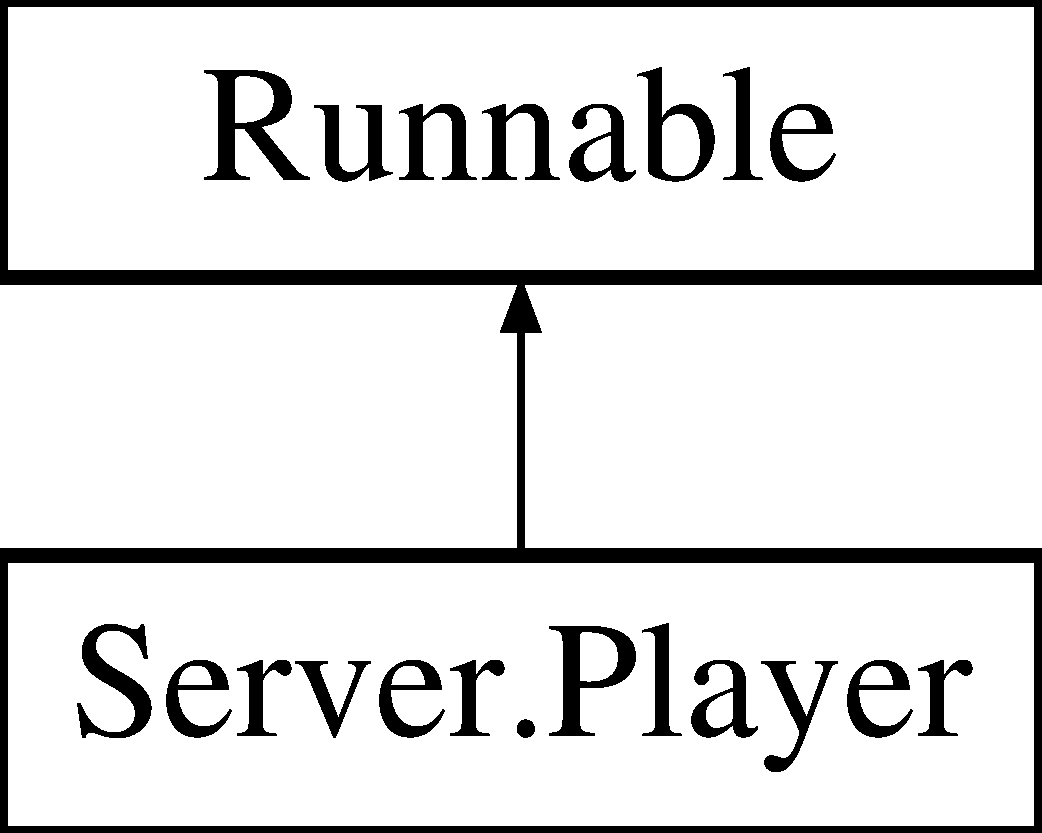
\includegraphics[height=2.000000cm]{a00073}
\end{center}
\end{figure}
\subsubsection*{Öffentliche Methoden}
\begin{DoxyCompactItemize}
\item 
\hyperlink{a00073_a858dba9ba878ab25863cad6e9b8bdbff}{Player} (\hyperlink{a00078}{Server} lobby\-Server, Object\-Output output, Object\-Input input)
\item 
void \hyperlink{a00073_aca6ecf908dbe1a01f04bf5d475c5e93d}{send} (\hyperlink{a00029}{Com\-Object} com)
\item 
void \hyperlink{a00073_a5d9f6a57cee2f22836f1ee65bf1be59c}{change\-Server} (\hyperlink{a00078}{Server} new\-Server)
\item 
String \hyperlink{a00073_ad23368a715fffac93891826bc9ec9034}{get\-Name} ()
\item 
void \hyperlink{a00073_a2ec69db14218d0d1b2ce9a2a1129b0d4}{set\-Name} (String new\-Name)
\end{DoxyCompactItemize}


\subsubsection{Ausführliche Beschreibung}
Sie verwaltet für die Dauer einer Serververbindung die Verbindung zum Client \begin{DoxyAuthor}{Autor}
Viktoria 
\end{DoxyAuthor}


\subsubsection{Beschreibung der Konstruktoren und Destruktoren}
\hypertarget{a00073_a858dba9ba878ab25863cad6e9b8bdbff}{\index{Server\-::\-Player@{Server\-::\-Player}!Player@{Player}}
\index{Player@{Player}!Server::Player@{Server\-::\-Player}}
\paragraph[{Player}]{\setlength{\rightskip}{0pt plus 5cm}Server.\-Player.\-Player (
\begin{DoxyParamCaption}
\item[{{\bf Server}}]{lobby\-Server, }
\item[{Object\-Output}]{output, }
\item[{Object\-Input}]{input}
\end{DoxyParamCaption}
)}}\label{a00073_a858dba9ba878ab25863cad6e9b8bdbff}


Konstruktor des Players, in ihm werden die Attribute server, com\-Out und Com\-In mit vom Client\-Listerer\-Thret übergebenen werten Instanziiert. 


\begin{DoxyParams}{Parameter}
{\em lobby\-Server} & ist der \hyperlink{a00054}{Lobby\-Server}, der zu Beginn den \hyperlink{a00073}{Player} verwaltet. \\
\hline
{\em output} & ist der Object\-Output an den entsprechenden Client \\
\hline
{\em input} & ist der Object\-Input vom entsprechenden Client \\
\hline
\end{DoxyParams}


\subsubsection{Dokumentation der Elementfunktionen}
\hypertarget{a00073_a5d9f6a57cee2f22836f1ee65bf1be59c}{\index{Server\-::\-Player@{Server\-::\-Player}!change\-Server@{change\-Server}}
\index{change\-Server@{change\-Server}!Server::Player@{Server\-::\-Player}}
\paragraph[{change\-Server}]{\setlength{\rightskip}{0pt plus 5cm}void Server.\-Player.\-change\-Server (
\begin{DoxyParamCaption}
\item[{{\bf Server}}]{new\-Server}
\end{DoxyParamCaption}
)}}\label{a00073_a5d9f6a57cee2f22836f1ee65bf1be59c}


Diese Methode wechselt beim \hyperlink{a00073}{Player} den \hyperlink{a00078}{Server} an den er com\-Objects weiterleiten soll. 

Dabei wird er aus dem player\-Set des alten Servers entfernt und in das player\-Set des neuen Players eingefugt. Danach wird vom neuen \hyperlink{a00078}{Server} ein Com\-Update\-Playerlist Objekt mit broadcast an alle Clients, die vom \hyperlink{a00078}{Server} verwaltet werden, verschickt. 
\begin{DoxyParams}{Parameter}
{\em new\-Server} & ist der neue \hyperlink{a00078}{Server} \\
\hline
\end{DoxyParams}
\hypertarget{a00073_ad23368a715fffac93891826bc9ec9034}{\index{Server\-::\-Player@{Server\-::\-Player}!get\-Name@{get\-Name}}
\index{get\-Name@{get\-Name}!Server::Player@{Server\-::\-Player}}
\paragraph[{get\-Name}]{\setlength{\rightskip}{0pt plus 5cm}String Server.\-Player.\-get\-Name (
\begin{DoxyParamCaption}
{}
\end{DoxyParamCaption}
)}}\label{a00073_ad23368a715fffac93891826bc9ec9034}


Getter-\/\-Methode für den Benutzernamen. 

\begin{DoxyReturn}{Rückgabe}
gibt den Benutzernamen des Spielers zurück 
\end{DoxyReturn}
\hypertarget{a00073_aca6ecf908dbe1a01f04bf5d475c5e93d}{\index{Server\-::\-Player@{Server\-::\-Player}!send@{send}}
\index{send@{send}!Server::Player@{Server\-::\-Player}}
\paragraph[{send}]{\setlength{\rightskip}{0pt plus 5cm}void Server.\-Player.\-send (
\begin{DoxyParamCaption}
\item[{{\bf Com\-Object}}]{com}
\end{DoxyParamCaption}
)}}\label{a00073_aca6ecf908dbe1a01f04bf5d475c5e93d}


Diese Methode schickt ein Com\-Objekt an den Client. 


\begin{DoxyParams}{Parameter}
{\em com} & ist das Com\-Object das verschickt wird \\
\hline
\end{DoxyParams}
\hypertarget{a00073_a2ec69db14218d0d1b2ce9a2a1129b0d4}{\index{Server\-::\-Player@{Server\-::\-Player}!set\-Name@{set\-Name}}
\index{set\-Name@{set\-Name}!Server::Player@{Server\-::\-Player}}
\paragraph[{set\-Name}]{\setlength{\rightskip}{0pt plus 5cm}void Server.\-Player.\-set\-Name (
\begin{DoxyParamCaption}
\item[{String}]{new\-Name}
\end{DoxyParamCaption}
)}}\label{a00073_a2ec69db14218d0d1b2ce9a2a1129b0d4}


Setter-\/\-Methode für den Benutzernamen. 


\begin{DoxyParams}{Parameter}
{\em new\-Name} & ist der neue Name \\
\hline
\end{DoxyParams}

\hypertarget{a00074}{\subsection{Ruleset.\-Player\-State Klassenreferenz}
\label{a00074}\index{Ruleset.\-Player\-State@{Ruleset.\-Player\-State}}
}
\subsubsection*{Öffentliche Methoden}
\begin{DoxyCompactItemize}
\item 
String \hyperlink{a00074_a20076c230bb4bfa3404b53bead5194d7}{get\-Name} ()
\item 
Array\-List$<$ \hyperlink{a00002}{Card} $>$ \hyperlink{a00074_a51f5e669f6c38b2810d833010a8fc6d0}{get\-Hand} ()
\item 
\hyperlink{a00069}{Other\-Data} \hyperlink{a00074_ad913d4462ff4019b1d85ba534a27250e}{get\-Other\-Data} ()
\item 
void \hyperlink{a00074_a613eaeb717801aca760df6776d34d228}{add\-Card} (\hyperlink{a00002}{Card} card)
\item 
boolean \hyperlink{a00074_ac8c5ede3e4788f8efd3527c16a7a696d}{remove\-Card} (\hyperlink{a00002}{Card} card)
\end{DoxyCompactItemize}


\subsubsection{Ausführliche Beschreibung}
Sie enthält den Namen des Spielers, seine Handkarten und \hyperlink{a00069}{Other\-Data}. 

\subsubsection{Dokumentation der Elementfunktionen}
\hypertarget{a00074_a613eaeb717801aca760df6776d34d228}{\index{Ruleset\-::\-Player\-State@{Ruleset\-::\-Player\-State}!add\-Card@{add\-Card}}
\index{add\-Card@{add\-Card}!Ruleset::PlayerState@{Ruleset\-::\-Player\-State}}
\paragraph[{add\-Card}]{\setlength{\rightskip}{0pt plus 5cm}void Ruleset.\-Player\-State.\-add\-Card (
\begin{DoxyParamCaption}
\item[{{\bf Card}}]{card}
\end{DoxyParamCaption}
)}}\label{a00074_a613eaeb717801aca760df6776d34d228}


Gibt dem Spieler eine Karte. 


\begin{DoxyParams}{Parameter}
{\em card} & Die Karte die dem Spieler gegeben wird \\
\hline
\end{DoxyParams}
\hypertarget{a00074_a51f5e669f6c38b2810d833010a8fc6d0}{\index{Ruleset\-::\-Player\-State@{Ruleset\-::\-Player\-State}!get\-Hand@{get\-Hand}}
\index{get\-Hand@{get\-Hand}!Ruleset::PlayerState@{Ruleset\-::\-Player\-State}}
\paragraph[{get\-Hand}]{\setlength{\rightskip}{0pt plus 5cm}Array\-List$<${\bf Card}$>$ Ruleset.\-Player\-State.\-get\-Hand (
\begin{DoxyParamCaption}
{}
\end{DoxyParamCaption}
)}}\label{a00074_a51f5e669f6c38b2810d833010a8fc6d0}


Holt die Kartenhand des Spielers. 

\begin{DoxyReturn}{Rückgabe}
own\-Hand Die Kartenhand des Spielers 
\end{DoxyReturn}
\hypertarget{a00074_a20076c230bb4bfa3404b53bead5194d7}{\index{Ruleset\-::\-Player\-State@{Ruleset\-::\-Player\-State}!get\-Name@{get\-Name}}
\index{get\-Name@{get\-Name}!Ruleset::PlayerState@{Ruleset\-::\-Player\-State}}
\paragraph[{get\-Name}]{\setlength{\rightskip}{0pt plus 5cm}String Ruleset.\-Player\-State.\-get\-Name (
\begin{DoxyParamCaption}
{}
\end{DoxyParamCaption}
)}}\label{a00074_a20076c230bb4bfa3404b53bead5194d7}


Holt den namen eines Spielers. 

\begin{DoxyReturn}{Rückgabe}
name Der Name des Spielers 
\end{DoxyReturn}
\hypertarget{a00074_ad913d4462ff4019b1d85ba534a27250e}{\index{Ruleset\-::\-Player\-State@{Ruleset\-::\-Player\-State}!get\-Other\-Data@{get\-Other\-Data}}
\index{get\-Other\-Data@{get\-Other\-Data}!Ruleset::PlayerState@{Ruleset\-::\-Player\-State}}
\paragraph[{get\-Other\-Data}]{\setlength{\rightskip}{0pt plus 5cm}{\bf Other\-Data} Ruleset.\-Player\-State.\-get\-Other\-Data (
\begin{DoxyParamCaption}
{}
\end{DoxyParamCaption}
)}}\label{a00074_ad913d4462ff4019b1d85ba534a27250e}


Holt die zusätzlichen Informationen des Spielers. 

\begin{DoxyReturn}{Rückgabe}
own\-Hand Die zusätzlichen Informationen des Spielers 
\end{DoxyReturn}
\hypertarget{a00074_ac8c5ede3e4788f8efd3527c16a7a696d}{\index{Ruleset\-::\-Player\-State@{Ruleset\-::\-Player\-State}!remove\-Card@{remove\-Card}}
\index{remove\-Card@{remove\-Card}!Ruleset::PlayerState@{Ruleset\-::\-Player\-State}}
\paragraph[{remove\-Card}]{\setlength{\rightskip}{0pt plus 5cm}boolean Ruleset.\-Player\-State.\-remove\-Card (
\begin{DoxyParamCaption}
\item[{{\bf Card}}]{card}
\end{DoxyParamCaption}
)}}\label{a00074_ac8c5ede3e4788f8efd3527c16a7a696d}


Entfernt eine Karte aus der Hand des Spielers. 


\begin{DoxyParams}{Parameter}
{\em card} & \\
\hline
\end{DoxyParams}
\begin{DoxyReturn}{Rückgabe}
own\-Hand.\-remove(card) Gibt true zurück wenn die Karte in der Hand ist und false sonst 
\end{DoxyReturn}

\hypertarget{a00075}{\subsection{Com\-Objects.\-Ruleset\-Message Klassenreferenz}
\label{a00075}\index{Com\-Objects.\-Ruleset\-Message@{Com\-Objects.\-Ruleset\-Message}}
}
Klassendiagramm für Com\-Objects.\-Ruleset\-Message\-:\begin{figure}[H]
\begin{center}
\leavevmode
\includegraphics[height=12.000000cm]{a00075}
\end{center}
\end{figure}


\subsubsection{Ausführliche Beschreibung}
Sie enthält einen Nachrichtentyp und vererbt an alle Nachrichten für das Regelwerk. 
\hypertarget{a00076}{\subsection{Ruleset.\-Ruleset\-Type Enum-\/\-Referenz}
\label{a00076}\index{Ruleset.\-Ruleset\-Type@{Ruleset.\-Ruleset\-Type}}
}

\hypertarget{a00077}{\subsection{Server Klassenreferenz}
\label{a00077}\index{Server@{Server}}
}


Basisklasse für \hyperlink{a00072}{Game\-Server} und \hyperlink{a00074}{Lobby\-Server}.

\subsubsection*{Öffentliche Methoden}
\begin{DoxyCompactItemize}
\item 
void \hyperlink{a00077_aab90f477a811b12d935c46ec7cbabb08}{receive\-Message} (\hyperlink{a00076}{Player} player, Com\-Object com)
\item 
synchronized void \hyperlink{a00077_ac90f610b90effa3a0cf572d3cbe270c3}{send\-To\-Player} (String name, Com\-Object com)
\item 
synchronized void \hyperlink{a00077_ac0a0163cec54e6202131c76962d7834b}{add\-Player} (\hyperlink{a00076}{Player} player)
\item 
synchronized void \hyperlink{a00077_a8b2712c19a20e54b3c5d99ce9d21112e}{remove\-Player} (\hyperlink{a00076}{Player} player)
\item 
synchronized void \hyperlink{a00077_aa5dbc77abbcc945c59d4edc75e55e7cf}{broadcast} (Com\-Object com)
\item 
void \hyperlink{a00077_af3ddb51daa156429385870eb04bd456e}{handle\-I\-O\-Exception} (\hyperlink{a00076}{Player} player)
\end{DoxyCompactItemize}
\subsubsection*{Geschützte Attribute}
\begin{DoxyCompactItemize}
\item 
\hypertarget{a00077_ab10ffe465a33e3a82e0132c97628b9a5}{Set$<$ \hyperlink{a00076}{Player} $>$ \hyperlink{a00077_ab10ffe465a33e3a82e0132c97628b9a5}{player\-Set}}\label{a00077_ab10ffe465a33e3a82e0132c97628b9a5}

\end{DoxyCompactItemize}


\subsubsection{Ausführliche Beschreibung}
Ist eine abstrakte Klasse, von der die Klassen \hyperlink{a00074}{Lobby\-Server} und \hyperlink{a00072}{Game\-Server} erben. Es stellt Methoden zur Nachrichtenversendung und -\/verarbeitung bereit, sowie zur Verwaltung von Playern 

\subsubsection{Dokumentation der Elementfunktionen}
\hypertarget{a00077_aab90f477a811b12d935c46ec7cbabb08}{\index{Server\-::\-Server@{Server\-::\-Server}!receive\-Message@{receive\-Message}}
\index{receive\-Message@{receive\-Message}!Server::Server@{Server\-::\-Server}}
\paragraph[{receive\-Message}]{\setlength{\rightskip}{0pt plus 5cm}void receive\-Message (
\begin{DoxyParamCaption}
\item[{{\bf Player}}]{player, }
\item[{Com\-Object}]{com}
\end{DoxyParamCaption}
)}}\label{a00077_aab90f477a811b12d935c46ec7cbabb08}


Diese Methode dient zur Verarbeitung von eingehenden Com\-Objects. 


\begin{DoxyParams}{Parameter}
{\em player} & ist der \hyperlink{a00076}{Player} von dem die Nachricht kommt \\
\hline
{\em com} & ist das Com\-Objekt vom Client verschickt wurde \\
\hline
\end{DoxyParams}
\hypertarget{a00077_ac90f610b90effa3a0cf572d3cbe270c3}{\index{Server\-::\-Server@{Server\-::\-Server}!send\-To\-Player@{send\-To\-Player}}
\index{send\-To\-Player@{send\-To\-Player}!Server::Server@{Server\-::\-Server}}
\paragraph[{send\-To\-Player}]{\setlength{\rightskip}{0pt plus 5cm}synchronized void send\-To\-Player (
\begin{DoxyParamCaption}
\item[{String}]{name, }
\item[{Com\-Object}]{com}
\end{DoxyParamCaption}
)}}\label{a00077_ac90f610b90effa3a0cf572d3cbe270c3}


Diese Methode wird genutzt, um ein Com\-Object an einen einzigen Client zu verschicken. 

Der \hyperlink{a00076}{Player} der die Nachricht verschicken soll wird Anhand des uebergebenen Benutzernamens identifiziert. Es wird vorrausgesetzt, dass der Name und das Com\-Object gueltig sind. 
\begin{DoxyParams}{Parameter}
{\em name} & ist der Name des Clients, an den der \hyperlink{a00076}{Player} die Nachricht verschicken soll \\
\hline
{\em c} & ist das Com\-Object, dass verschickt werden soll \\
\hline
\end{DoxyParams}


Benutzt Server.\-player\-Set.



Wird benutzt von Game\-Server.\-send\-Ruleset\-Message().

\hypertarget{a00077_ac0a0163cec54e6202131c76962d7834b}{\index{Server\-::\-Server@{Server\-::\-Server}!add\-Player@{add\-Player}}
\index{add\-Player@{add\-Player}!Server::Server@{Server\-::\-Server}}
\paragraph[{add\-Player}]{\setlength{\rightskip}{0pt plus 5cm}synchronized void add\-Player (
\begin{DoxyParamCaption}
\item[{{\bf Player}}]{player}
\end{DoxyParamCaption}
)}}\label{a00077_ac0a0163cec54e6202131c76962d7834b}


Diese Methode fuegt einen \hyperlink{a00076}{Player} dem Set an Playern hinzu, welche der \hyperlink{a00077}{Server} verwaltet. 

Es wird vorrausgesetzt, dass der \hyperlink{a00076}{Player} gueltig und noch nicht im Set vorhanden ist. 
\begin{DoxyParams}{Parameter}
{\em player} & ist der \hyperlink{a00076}{Player}, der hinzugefuegt wird \\
\hline
\end{DoxyParams}
\hypertarget{a00077_a8b2712c19a20e54b3c5d99ce9d21112e}{\index{Server\-::\-Server@{Server\-::\-Server}!remove\-Player@{remove\-Player}}
\index{remove\-Player@{remove\-Player}!Server::Server@{Server\-::\-Server}}
\paragraph[{remove\-Player}]{\setlength{\rightskip}{0pt plus 5cm}synchronized void remove\-Player (
\begin{DoxyParamCaption}
\item[{{\bf Player}}]{player}
\end{DoxyParamCaption}
)}}\label{a00077_a8b2712c19a20e54b3c5d99ce9d21112e}


Diese Methode entfernt einen \hyperlink{a00076}{Player} aus dem Set an Playern, welche der \hyperlink{a00077}{Server} verwaltet. 

Es wird vorrausgesetzt, dass der \hyperlink{a00076}{Player} gueltig und im Set vorhanden ist. 
\begin{DoxyParams}{Parameter}
{\em player} & ist der \hyperlink{a00076}{Player}, der entfernt wird \\
\hline
\end{DoxyParams}
\hypertarget{a00077_aa5dbc77abbcc945c59d4edc75e55e7cf}{\index{Server\-::\-Server@{Server\-::\-Server}!broadcast@{broadcast}}
\index{broadcast@{broadcast}!Server::Server@{Server\-::\-Server}}
\paragraph[{broadcast}]{\setlength{\rightskip}{0pt plus 5cm}synchronized void broadcast (
\begin{DoxyParamCaption}
\item[{Com\-Object}]{com}
\end{DoxyParamCaption}
)}}\label{a00077_aa5dbc77abbcc945c59d4edc75e55e7cf}


Diese Methode wird genutzt, um ein Com\-Object an alle Clients, die vom \hyperlink{a00077}{Server} verwaltet werden, zu schicken. 

Es wird vorrausgesetzt, dass das Com\-Object gueltig ist. 
\begin{DoxyParams}{Parameter}
{\em com} & ist das Com\-Object, dass verschickt werden soll \\
\hline
\end{DoxyParams}


Benutzt Server.\-player\-Set.



Wird benutzt von Game\-Server.\-broadcast\-Ruleset\-Message(), Lobby\-Server.\-receive\-Message() und Game\-Server.\-receive\-Message().

\hypertarget{a00077_af3ddb51daa156429385870eb04bd456e}{\index{Server\-::\-Server@{Server\-::\-Server}!handle\-I\-O\-Exception@{handle\-I\-O\-Exception}}
\index{handle\-I\-O\-Exception@{handle\-I\-O\-Exception}!Server::Server@{Server\-::\-Server}}
\paragraph[{handle\-I\-O\-Exception}]{\setlength{\rightskip}{0pt plus 5cm}void handle\-I\-O\-Exception (
\begin{DoxyParamCaption}
\item[{{\bf Player}}]{player}
\end{DoxyParamCaption}
)}}\label{a00077_af3ddb51daa156429385870eb04bd456e}


Diese Methode legt den Ablauf fest, was passiert, falls die Verbindung zu einem Client verloren gegangen ist. 


\begin{DoxyParams}{Parameter}
{\em player} & ist der Tread von dem die I\-O\-Exception kommt \\
\hline
\end{DoxyParams}

\hypertarget{a00078}{\subsection{Server\-Main Klassenreferenz}
\label{a00078}\index{Server\-Main@{Server\-Main}}
}
\subsubsection*{Öffentliche, statische Methoden}
\begin{DoxyCompactItemize}
\item 
static void \hyperlink{a00078_a8b260eecbaabcef8473fd87ada040682}{main} (String\mbox{[}$\,$\mbox{]} args)
\end{DoxyCompactItemize}
\subsubsection*{Private Attribute}
\begin{DoxyCompactItemize}
\item 
\hypertarget{a00078_a9cb4ab84f6237f795298724e3d6f4da8}{\hyperlink{a00074}{Lobby\-Server} \hyperlink{a00078_a9cb4ab84f6237f795298724e3d6f4da8}{lobby\-Server}}\label{a00078_a9cb4ab84f6237f795298724e3d6f4da8}

\end{DoxyCompactItemize}


\subsubsection{Ausführliche Beschreibung}
Diese Klasse startet den \hyperlink{a00077}{Server} und ist fuer die Konfiguration des Servers verantwortlich. 

\subsubsection{Dokumentation der Elementfunktionen}
\hypertarget{a00078_a8b260eecbaabcef8473fd87ada040682}{\index{Server\-::\-Server\-Main@{Server\-::\-Server\-Main}!main@{main}}
\index{main@{main}!Server::ServerMain@{Server\-::\-Server\-Main}}
\paragraph[{main}]{\setlength{\rightskip}{0pt plus 5cm}static void main (
\begin{DoxyParamCaption}
\item[{String\mbox{[}$\,$\mbox{]}}]{args}
\end{DoxyParamCaption}
)\hspace{0.3cm}{\ttfamily [static]}}}\label{a00078_a8b260eecbaabcef8473fd87ada040682}


Die main-\/\-Methode erstellt einen neuen \hyperlink{a00074}{Lobby\-Server}. 


\begin{DoxyParams}{Parameter}
{\em args} & \\
\hline
\end{DoxyParams}

%--- End generated contents ---
\section{JUnit-Tests}
JUnit-Tests werden für die folgenden Klassen geschrieben: ClientModel, LobbyServer,
GameServer, ClientHearts, ClientWizard, ServerHearts und ServerWizard. Für die folgenden Fälle wurden bereits Tests implementier.

\subsection{isValidWizardMove}
\begin{lstlisting}
package Ruleset;


import static org.junit.Assert.assertFalse;
import static org.junit.Assert.assertTrue;

import org.junit.After;
import org.junit.Before;
import org.junit.Test;

import test.TestGameServer;
import test.TestLobbyServer;
import test.TestPlayer;

import Server.GameServer;
import Server.LobbyServer;
import Server.Player;

public class TestisValidMoveWizard {
	
	ServerRuleset ruleset;
	
	GameServer gameServer;
	
	LobbyServer lobbyServer;
	
	Player player;
	String player1;
	String player2;
	String player3;
	PlayerState playerState1;
	PlayerState playerState2;
	PlayerState playerState3;
	
	@Before
	public void setUp() throws Exception {
		player1 = "Tick";
		player2 = "Trick";
		player3 = "Track";
		lobbyServer = new TestLobbyServer();
		player = new TestPlayer(lobbyServer,null,null);
		gameServer = new TestGameServer(lobbyServer,player,"Mein Spiel",RulesetType.Wizard, 
				"",false);
		ruleset = new ServerWizard(gameServer);
		
		ruleset.addPlayerToGame(player1);
		ruleset.addPlayerToGame(player2);
		ruleset.addPlayerToGame(player3);
		
		playerState1 = ruleset.getPlayerState(player1);
		playerState2 = ruleset.getPlayerState(player2);
		playerState3 = ruleset.getPlayerState(player3);
		
		ruleset.setFirstPlayer(ruleset.getPlayerState(player1));
		ruleset.setTrumpCard(WizardCard.VierRot);
		
		ruleset.giveACard(playerState1, WizardCard.DreiGruen);
		ruleset.giveACard(playerState1, WizardCard.ZaubererRot);
		ruleset.givaACard(playerState1, WizardCard.ZweiBlau);
		
		ruleset.giveACard(playerState2, WizardCard.ZweiGruen);
		ruleset.giveACard(playerState2, WizardCard.DreiRot);
		ruleset.givaACard(playerState2, WizardCard.ZweiGelb);
		
		ruleset.giveACard(playerState3, WizardCard.NarrBlau);
		ruleset.giveACard(playerState3, WizardCard.EinsGruen);
		ruleset.giveACard(playerState3, WizardCard.ZweiRot);
	}
	
	@Test
	public void testSorcerer() {
		ruleset.playCard(WizardCard.ZaubererRot);
		ruleset.setCurrentPlayer(playerState2);
		
		boolean isValidMove = ruleset.isValidMove(WizardCard.DreiRot);
		
		assertTrue(isValidMove);
	}
	
	@Test
	public void testRed3OnGreen3() {
		ruleset.playCard(WizardCard.DreiGruen);
		ruleset.setCurrentPlayer(playerState2);
		boolean isValidMove = ruleset.isValidMove(WizardCard.DreiRot);
		
		assertFalse(isValidMove);
	}
	
	@Test
	public void testGreen2OnGreen3() {
		ruleset.playCard(WizardCard.DreiGruen);
		ruleset.setCurrentPlayer(playerState2);
		
		boolean isValidMove = ruleset.isValidMove(WizardCard.ZweiGruen);
		
		assertTrue(isValidMove);
	}
	
	@Test
	public void testFoolBlueOnGreen2OnGreen3() {
		ruleset.playCard(WizardCard.DreiGruen);
		ruleset.setCurrentPlayer(playerState2);
		
		ruleset.playCard(WizardCard.ZweiGruen);
		ruleset.setCurrentPlayer(playerState3);
		
		boolean isValidMove = ruleset.isValidMove(WizardCard.NarrBlau);
		
		assertTrue(isValidMove);
	}

}
\end{lstlisting}

\subsection{isValidHeartsMove}
\begin{lstlisting}
package Ruleset;


import static org.junit.Assert.*;
import static org.junit.Assert.assertEquals;

import org.junit.Before;
import org.junit.Test;

import test.TestGameServer;
import test.TestLobbyServer;
import test.TestPlayer;

import Server.GameServer;
import Server.LobbyServer;
import Server.Player;

public class TestisValidMoveHearts {
	ServerRuleset ruleset;
	
	GameServer gameServer;
	
	LobbyServer lobbyServer;
	
	Player player;
	String player1;
	String player2;
	String player3;
	String player4;
	
	PlayerState playerState1;
	PlayerState playerState2;
	PlayerState playerState3;
	PlayerState playerState4;
	
	@Before
	public void setUp() throws Exception {
		player1 = "Tick";
		player2 = "Trick";
		player3 = "Track";
		player3 = "Duck";
		lobbyServer = new TestLobbyServer();
		player = new TestPlayer(lobbyServer,null,null);
		gameServer = new TestGameServer(lobbyServer,player,"Mein Spiel",
				RulesetType.Hearts, "",false);
		ruleset = new ServerHearts(gameServer);
		
		ruleset.addPlayerToGame(player1);
        ruleset.addPlayerToGame(player2);
        ruleset.addPlayerToGame(player3);
        ruleset.addPlayerToGame(player4);
        
        playerState1 = ruleset.getPlayerState(player1);
        playerState2 = ruleset.getPlayerState(player2);
        playerState3 = ruleset.getPlayerState(player3);

        ruleset.setFirstPlayer(playerState1);
	}
	
	@Test
	public void testIsValidMove() {
		 ruleset.giveACard(playerState1, HeartsCard.Herz2);
	     ruleset.giveACard(playerState1, HeartsCard.Kreuz9);
	     ruleset.giveACard(playerState2, HeartsCard.Caro3);
	     ruleset.giveACard(playerState2, HeartsCard.Caro6);
	     ruleset.giveACard(playerState3, HeartsCard.Pik4);
	     ruleset.giveACard(playerState3, HeartsCard.Pik5);
         ruleset.giveACard(playerState4, HeartsCard.Pik1);
	     ruleset.giveACard(playerState4, HeartsCard.Herz7);
	     
	     boolean isValidMove = ruleset.isValidMove(HeartsCard.Herz2);

	     assertFalse(isValidMove);

	     boolean isValidMove2 = ruleset.isValidMove(HeartsCard.Caro3);
	     
	     assertTrue(isValidMove2);
	}
	
	@Test
	public void testIsValidMoveOnlyHearts() {
		 ruleset.giveACard(playerState1, HeartsCard.Herz2);
	     ruleset.giveACard(playerState1, HeartsCard.Herz5);
	     ruleset.giveACard(playerState2, HeartsCard.Caro3);
	     ruleset.giveACard(playerState2, HeartsCard.Caro6);
	     ruleset.giveACard(playerState3, HeartsCard.Pik4);
	     ruleset.giveACard(playerState3, HeartsCard.Pik5);
         ruleset.giveACard(playerState4, HeartsCard.Pik1);
	     ruleset.giveACard(playerState4, HeartsCard.Herz7);
	     
	     boolean isValidMove = ruleset.isValidMove(HeartsCard.Herz2);

	     assertTrue(isValidMove);

	     boolean isValidMove2 = ruleset.isValidMove(HeartsCard.Herz5);
	     
	     assertTrue(isValidMove2);
	}

}
\end{lstlisting}

\subsection{getWinner}
\begin{lstlisting}
package Ruleset;

import static org.junit.Assert.*;

import java.util.List;

import org.junit.After;
import org.junit.Before;
import org.junit.Test;
import testKlassen.TestPlayer;
import ComObjects.ComObject;
import ComObjects.ComRuleset;
import ComObjects.MsgGameEnd;
import Server.GameServer;
import Server.LobbyServer;
import Server.Player;

public class TestHeartsWinner {

LobbyServer lobbyServer;
	
	GameServer gameServer;
	
	ServerRuleset heartsServerRuleset;
	
	TestPlayer blue;
	
	TestPlayer white;
	
	TestPlayer orange;
	
	TestPlayer brown;
	
	List<ComObject> inputList;
	
	ComRuleset comObject;
	
	MsgGameEnd endMsg;
	
	String winner;
	
	@Before
	public void setUp() {
		lobbyServer = new LobbyServer();
		blue = new TestPlayer(lobbyServer, null, null);
		white = new TestPlayer(lobbyServer, null, null);
		orange = new TestPlayer(lobbyServer, null, null);
		brown = new TestPlayer(lobbyServer, null, null);
	}
	
	@After
	public void tearDown() {	
		blue = null;
		white = null;
		orange = null;
		brown = null;
		lobbyServer = null;
		gameServer = null;
		inputList = null;
		comObject = null;
		endMsg = null;
		winner = null;
	}
	
	@Test
	public void testGetWinner() {
		
		gameServer = new GameServer(lobbyServer, blue, "Test Game", RulesetType.Wizard, "", false);
		gameServer.addPlayer(white);
		gameServer.addPlayer(orange);
		gameServer.addPlayer(brown);
		
		heartsServerRuleset = new ServerWizard(gameServer);
		heartsServerRuleset.addPlayerToGame("Mr. Blue");
		heartsServerRuleset.addPlayerToGame("Mr. White");
		heartsServerRuleset.addPlayerToGame("Mr. Orange");
		heartsServerRuleset.addPlayerToGame("Mr. Brown");
		heartsServerRuleset.setPoints(heartsServerRuleset.getPlayerState("Mr. Blue"),80);
		heartsServerRuleset.setPoints(heartsServerRuleset.getPlayerState("Mr. White"),20);
		heartsServerRuleset.setPoints(heartsServerRuleset.getPlayerState("Mr. Orange"),60);
		heartsServerRuleset.setPoints(heartsServerRuleset.getPlayerState("Mr. Brown"),110);
		heartsServerRuleset.setGamePhase(GamePhase.Ending);
		heartsServerRuleset.calculateRoundOutcome();
		
		assertTrue(heartsServerRuleset.getWinner().equals("Mr. Brown"));
		
		inputList = blue.getServerInput();
		comObject = (ComRuleset) inputList.get(1);
		endMsg = (MsgGameEnd) comObject.getRulesetMessage();
		winner = endMsg.getWinner();
		assertEquals("Nachricht an Blue", "Mr. Brown", winner);

		inputList = white.getServerInput();
		comObject = (ComRuleset) inputList.get(1);
		endMsg = (MsgGameEnd) comObject.getRulesetMessage();
		winner = endMsg.getWinner();
		assertEquals("Nachricht an White", "Mr. Brown", winner);

		inputList = orange.getServerInput();
		comObject = (ComRuleset) inputList.get(1);
		endMsg = (MsgGameEnd) comObject.getRulesetMessage();
		winner = endMsg.getWinner();
		assertEquals("Nachricht an Orange", "Mr. Brown", winner);
	
		inputList = brown.getServerInput();
		comObject = (ComRuleset) inputList.get(1);
		endMsg = (MsgGameEnd) comObject.getRulesetMessage();
		winner = endMsg.getWinner();
		assertEquals("Nachricht an Brown", "Mr. Brown", winner);
	}
}
\end{lstlisting}

\begin{lstlisting}
package Ruleset;

import static org.junit.Assert.*;

import java.util.List;

import org.junit.After;
import org.junit.Before;
import org.junit.Test;
import testKlassen.TestPlayer;
import ComObjects.ComChatMessage;
import ComObjects.ComObject;
import ComObjects.ComRuleset;
import ComObjects.MsgGameEnd;
import Server.GameServer;
import Server.LobbyServer;

/**
 * Testet ob der richtige Sieger ermittelt wird und ob jedem Mitspieler
 * der richtige Sieger mitgeteilt wird
 */
public class TestWizardWinner {

	LobbyServer lobbyServer;
	
	GameServer gameServer;
	
	ServerRuleset wizardServerRuleset;
	
	TestPlayer blue;
	
	TestPlayer white;
	
	TestPlayer orange;
	
	TestPlayer brown;
	
	List<ComObject> inputList;
	
	ComRuleset comObject;
	
	MsgGameEnd endMsg;
	
	String winner;
	
	@Before
	public void setUp() {
		lobbyServer = new LobbyServer();
		blue = new TestPlayer(lobbyServer, null, null);
		white = new TestPlayer(lobbyServer, null, null);
		orange = new TestPlayer(lobbyServer, null, null);
		brown = new TestPlayer(lobbyServer, null, null);
	}
	
	@After
	public void tearDown() {	
		blue = null;
		white = null;
		orange = null;
		brown = null;
		lobbyServer = null;
		gameServer = null;
		inputList = null;
		inputList = null;
		comObject = null;
		endMsg = null;
		winner = null;
	}
	
	@Test
	public void testGetWinner() {
		
		gameServer = new GameServer(lobbyServer, blue, "Test Game", RulesetType.Wizard, "", false);
		gameServer.addPlayer(white);
		gameServer.addPlayer(orange);
		gameServer.addPlayer(brown);
		
		wizardServerRuleset = new ServerWizard(gameServer);
		wizardServerRuleset.addPlayerToGame("Mr. Blue");
		wizardServerRuleset.addPlayerToGame("Mr. White");
		wizardServerRuleset.addPlayerToGame("Mr. Orange");
		wizardServerRuleset.addPlayerToGame("Mr. Brown");
		wizardServerRuleset.setPoints(wizardServerRuleset.getPlayerState("Mr. Blue"),80);
		wizardServerRuleset.setPoints(wizardServerRuleset.getPlayerState("Mr. White"),200);
		wizardServerRuleset.setPoints(wizardServerRuleset.getPlayerState("Mr. Orange"),130);
		wizardServerRuleset.setPoints(wizardServerRuleset.getPlayerState("Mr. Brown"),240);
		wizardServerRuleset.setGamePhase(GamePhase.Ending);
		wizardServerRuleset.calculateRoundOutcome();
		
		assertTrue(wizardServerRuleset.getWinner().equals("Mr. Brown"));
		
		inputList = blue.getServerInput();
		comObject = (ComRuleset) inputList.get(1);
		endMsg = (MsgGameEnd) comObject.getRulesetMessage();
		winner = endMsg.getWinner();
		assertEquals("Nachricht an Blue", "Mr. Brown", winner);

		inputList = white.getServerInput();
		comObject = (ComRuleset) inputList.get(1);
		endMsg = (MsgGameEnd) comObject.getRulesetMessage();
		winner = endMsg.getWinner();
		assertEquals("Nachricht an White", "Mr. Brown", winner);

		inputList = orange.getServerInput();
		comObject = (ComRuleset) inputList.get(1);
		endMsg = (MsgGameEnd) comObject.getRulesetMessage();
		winner = endMsg.getWinner();
		assertEquals("Nachricht an Orange", "Mr. Brown", winner);
	
		inputList = brown.getServerInput();
		comObject = (ComRuleset) inputList.get(1);
		endMsg = (MsgGameEnd) comObject.getRulesetMessage();
		winner = endMsg.getWinner();
		assertEquals("Nachricht an Brown", "Mr. Brown", winner);
	}
}

\end{lstlisting}

\subsection{QuitPlayer}
\begin{lstlisting}
ackage Server;


import static org.junit.Assert.*;

import java.io.BufferedInputStream;
import java.io.IOException;
import java.io.ObjectInputStream;
import java.io.ObjectOutputStream;
import java.util.ArrayList;
import java.util.List;

import org.junit.After;
import org.junit.Before;
import org.junit.Test;

import test.TestGameServer;
import test.TestLobbyServer;
import test.TestPlayer;

import ComObjects.*;
import ComObjects.ComWarning;
import Ruleset.RulesetType;

public class QuitGameTest {

	TestLobbyServer lobby;
	
	TestPlayer player1; 
	
	TestPlayer player2; 
	TestPlayer player3;
	TestPlayer player4;
	
	TestGameServer game;
	
	ComClientQuit quit;
	
	@Before
	public void setUp() throws Exception {
		lobby = new TestLobbyServer();
		
		player1 = new TestPlayer(lobby, null, null);
		player1.setName("MrBlue");
		lobby.addPlayer(player1);
		
		player2 = new TestPlayer(lobby, null, null);
		player2.setName("MrWhite");
		player3 = new TestPlayer(lobby, null, null);
		player3.setName("MrPink");
		player4 = new TestPlayer(lobby, null, null);
		player4.setName("MrRed");
		
		game = new TestGameServer(lobby, player1, "MrBluesGame", RulesetType.Hearts, null, false);
		
		game.addPlayer(player2);
		game.addPlayer(player3);
		game.addPlayer(player4);
		
		quit = new ComClientQuit();
	}

	@After
	public void tearDown() throws Exception {
		lobby = null;
		player1 = null;
		player2 = null;
		player3 = null;
		player4 = null;
		game = null;
	}
	
	@Test
	public void testPlayerQuitGame() throws IOException{ 
		
		player1.changeServer(game);
		assertTrue(game.initLobby().getPlayerList().contains(player1.getName()));
		
		ComInitLobby initLobby = lobby.initLobby();
		ComWarning warning = new ComWarning("Ein Spieler hat das Spiel verlassen");
		
		player1.injectComObject(quit);

		assertFalse(lobby.initLobby().getGameList().contains(game));
		assertTrue(lobby.initLobby().getPlayerList().contains(player1.getName()));
		assertTrue(lobby.initLobby().getPlayerList().contains(player1.getName()));
		assertTrue(lobby.initLobby().getPlayerList().contains(player1.getName()));
		assertTrue(lobby.initLobby().getPlayerList().contains(player1.getName()));
		
		assertTrue(player1.getServerInput().get(0).getClass() == initLobby.getClass());
		assertTrue(player1.getServerInput().get(1).getClass() == warning.getClass());
		assertTrue(player2.getServerInput().get(0).getClass() == initLobby.getClass());
		assertTrue(player2.getServerInput().get(1).getClass() == warning.getClass());
		assertTrue(player3.getServerInput().get(0).getClass() == initLobby.getClass());
		assertTrue(player3.getServerInput().get(1).getClass() == warning.getClass());
		assertTrue(player4.getServerInput().get(0).getClass() == initLobby.getClass());
		assertTrue(player4.getServerInput().get(1).getClass() == warning.getClass());
	}
}
\end{lstlisting}

\subsection{Chat}

\begin{lstlisting}
package chat;

import static org.junit.Assert.*;

import org.junit.Test;
import org.junit.After;
import org.junit.Before;

import testKlassen.TestMessageListenerThread;
import testKlassen.TestObserver;
import Client.MessageListenerThread;
import Client.ClientModel;
import ComObjects.ComChatMessage;

public class ClientModelChatTest {

	ComChatMessage testMessage;
	
	ClientModel testModel;
	
	TestObserver testObserver;
	
	TestMessageListenerThread testNetIO;
	
	String testText;
	
	@Before  
    public void setUp() {
		testNetIO = new TestMessageListenerThread();
		testObserver = new TestObserver();
		testMessage = new ComChatMessage("Hello Test!");
		testModel = new ClientModel((MessageListenerThread) testNetIO);
		testNetIO.setModel(testModel);
		testModel.addObserver(testObserver);
    }  
  
    @After  
    public void tearDown() { 
    	testNetIO = null;
    	testMessage = null;
    	testModel = null;
    	testObserver = null;
    }  
	
	@Test
	public void testSendChatMessage() {
		String inputText = "Hello Test!";
		testModel.sendChatMessage(inputText);
		testText = ((ComChatMessage) testNetIO.getModelInput().get(0)).getChatMessage();
		assertEquals("Vergleich der gesendeten Chatnachrichten", testText, inputText);
	}
	
	@Test
	public void testReceiveChatMessage() {
		testNetIO.injectComObject(testMessage);
		assertTrue("Vergleich der empfangenen Chatnachrichten", 
				testObserver.getChatMessage().equals(testMessage.getChatMessage()));
	}
}
\end{lstlisting}

\begin{lstlisting}
package chat;

import static org.junit.Assert.*;

import org.junit.After;
import org.junit.Before;
import org.junit.Test;

import testKlassen.TestPlayer;
import Server.LobbyServer;
import ComObjects.ComChatMessage;

public class LobbyServerChatTest {

	ComChatMessage testMessage;
	
	LobbyServer testServer;

	TestPlayer player1;
	
	TestPlayer player2;
	
	TestPlayer player3;
	
	String testText1;
	
	String testText2;
	
	String testText3;

	@Before
	public void setUp() {
		testMessage = new ComChatMessage("Hello Test!");
		testServer = new LobbyServer();
		player1 = new TestPlayer(testServer, null, null);
		player2 = new TestPlayer(testServer, null, null);
		player3 = new TestPlayer(testServer, null, null);
	}

	@After
	public void tearDown() {
		testMessage = null;
		testServer = null;
		player1 = null;
		player2 = null;
		player3 = null;
		testText1 = null;
		testText2 = null;
		testText3 = null;
	}

	@Test
	public void testReceiveMessagePlayerComChatMessage() {
		String messageToMatch = testMessage.getChatMessage();
		testServer.addPlayer(player1);
		testServer.addPlayer(player2);
		testServer.addPlayer(player3);
		player1.injectComObject(testMessage);
		testText1 = ((ComChatMessage) player1.getServerInput()).getChatMessage();
		testText2 = ((ComChatMessage) player2.getServerInput()).getChatMessage();
		testText3 = ((ComChatMessage) player3.getServerInput()).getChatMessage();
		assertEquals("Nachricht an Spieler 1", messageToMatch, testText1);
		assertEquals("Nachricht an Spieler 2", messageToMatch, testText2);
		assertEquals("Nachricht an Spieler 3", messageToMatch, testText3);
	}
}

\end{lstlisting}

\section{Implementierungsplan}
Es werden für jeden Milestone die einzelnen Arbeitspakete angegeben. Die angegebenen Klassen werden nicht sofort vollständig implmentiert, sondern mit den vom Arbeitspaket und Milestone verlangten Funktionen ausgestattet.\\

\subsection{Milestone 1}
Für den ersten Milestone werden folgende Funktionen angestrebt:\\
Der Nutzer kann sich im Login-Fenster anmelden und die Lobby betreten. Er kann ein Spiel erstellen und offenen Spielen beitreten. Das wird in der Lobby angezeigt, man gelangt jedoch noch nicht ins Wartefenster. Nebenläufig dazu wird die Datenschicht der Regelwerke implementiert.\\ 
\begin{itemize}
\item View(Login+Lobby) Dauer: 8 Std. \\
Klassen: Login, Lobby, Warning, ClientController
\item Client(Login) Dauer 8 Std. \\
Klassen: ClientMain, ClientModel, MessageListener Thread, ClientState, ViewNotification
\item Server(Login) Dauer 16 Std. \\
Klassen: Server, ServerMain, LobbyServer, Player, ClientListenerThread, ComObject, ComLoginRequest, ComClientQuit, ComServerAcknowledgement, ComWarning
\item Ruleset(Daten) Dauer 20 Std. \\
Klassen:  Card, Colour, HeartsCard, WizCard, OtherData, WizData, HeartsData, GameClientUpdate, GameState, PlayerState, RulesetType
\item Client(Lobby) Dauer 8 Std. \\
Klassen: ClientModel
\item Server(Lobby) Dauer 8 Std. \\
Klassen: LobbyServer, ComChatMessage, ComLobbyUpdateGamelist, ComJoinRequest, ComInitLobby, ComUpdatePlayerlist
\item View(Create+Join) Dauer 8 Std. \\
Klassen: Password, CreateGame, ClientController
\item Client(Create+Join) Dauer 8 Std. \\
Klassen: ClientModel
\item Server(Create+Join) Dauer 12 Std. \\
Klassen: LobbyServer, ComJoinRequest, ComCreateGameRequest
\end{itemize}

\subsection{Milestone 2}
Für den zweiten Milestone werden folgende Funktionen angestrebt:\\
Beim Beitreten oder Erstellen eines Spiels gelangt man ins Wartefenster. Der Spielleiter kannn hier Spieler entfernen. Diese gelangen zurück in die Lobby. Das Spiel kann noch nicht gestartet werden, aber das Regelwerk wird bereits serverseitig implementiert.\\
\begin{itemize}
\item Ruleset(Wizard-Server) Dauer 30 Std. \\
Klassen: ServerRuleset, ServerWizard, RulesetMessage, MsgCard, MsgCardRequest, MsgGameEnd, MsgNumber, Msg NumberRequest, MsgSelection, MsgSelectionRequest, MsgUser
\item View(GameLobby) Dauer 8 Std. \\
Klassen: GameLobby, ClientController
\item Client(GameLobby) Dauer 8 Std. \\
Klassen: ClientModel
\item Server(GameLobby) Dauer 10 Std. \\
KLassen: LobbyServer, GameServer, ComBeenKicked, ComClientLeave, ComInitGameLobby, ComKickPlayerRequest, ComStartGame
\item View(Game) Dauer 20 Std. \\
Klassen: Game, GamePanel, OtherPlayer, OwnHand, ViewCard, DrawDeck, DiscardPile, ScoreWindow, ClientController
\item Client(Game) Dauer 14 Std. \\
Klassen: ClientModel
\end{itemize}

\subsection{Milestone 3}
Für den dritten Milestone werden folgende Funktionen angestrebt:\\
Es kann schon eine vollständige Partie Wizard gespielt werden.\\
\begin{itemize}
\item Server(Game) Dauer 4 Std. \\
Klassen: GameServer, ComStartGame, ComRuleset, ComGameEnd
\item Ruleset(Wizard-Client) Dauer 12 Std. \\
Klassen: ClientWizard
\item View(WizardWindows) Dauer 4 Std. \\
Klassen: ChooseItem, InputNumber, ClientController
\item Client(Wizard) Dauer 6 Std. \\
Klassen: ClientModel
\item View(HeartsWindows) Dauer 2 Std. \\
Klassen: ChooseCards, ClientController
\item Client(Hearts) Dauer 4 Std. \\
Klassen: ClientModel
\item Ruleset(Hearts-Server) Dauer 16 Std. \\
Klassen: ServerHearts
\end{itemize}

\subsection{Finale Version}
Die finale Version enthält die volle Funktionalität des Programs.
Es können also sowohl Wizard als auch Hearts gespielt werden.\\
\begin{itemize}
\item Ruleset(Hearts-Client) Dauer 10Std. \\
Klassen: ClientHearts
\item ViewPolishing(evtl Tests) Dauer 10Std \\
Verbesserungen an der bisherigen Implementierung. Gegebenfalls Schreiben von zusätzlichen Tests
\item ClientPolishing(evtl Tests) Dauer 10Std \\
Verbesserungen an der bisherigen Implementierung. Gegebenfalls Schreiben von zusätzlichen Tests
\item ServerPolishing(evtl Tests) Dauer 10Std \\
Verbesserungen an der bisherigen Implementierung. Gegebenfalls Schreiben von zusätzlichen Tests
\item RulesetPolishing(evtl Tests) Dauer 10Std \\
Verbesserungen an der bisherigen Implementierung. Gegebenfalls Schreiben von zusätzlichen Tests
\end{itemize}
\newpage

\subsection{Gantt-Diagramme}
\hspace*{-0.2\textwidth}Milestone 1: \\ \\
\hspace*{-0.2\textwidth}\includegraphics[width=1.4\textwidth]{Milestone1} \\ \\

\hspace*{-0.2\textwidth}Milestone 2: \\ \\
\hspace*{-0.2\textwidth}\includegraphics[width=1.4\textwidth]{Milestone2} \\ \\

\hspace*{-0.2\textwidth}Milestone 3: \\ \\
\hspace*{-0.2\textwidth}\includegraphics[width=1.4\textwidth]{Milestone3} \\ \\

\hspace*{-0.2\textwidth}Finale Version: \\ \\
\hspace*{-0.2\textwidth}\includegraphics[width=1.4\textwidth]{Milestone4} \\ \\
% Index
\newpage
\phantomsection
\addcontentsline{toc}{part}{Index}
\printindex

\end{document}
